\NeedsTeXFormat{LaTeX2e}
%-----------------------------------------------------------
\documentclass[a4paper,12pt]{monografia}
\usepackage[portuguese, colorinlistoftodos, textsize=tiny]{todonotes}
\usepackage{amsmath,amsthm,amsfonts,amssymb}

\usepackage{latexsym}
\usepackage[portuguese]{babel}  
\usepackage[utf8]{inputenc}
\usepackage{setspace}
%\usepackage{natbib}
\usepackage{bm}
\usepackage[portuguese,algoruled,longend, linesnumbered]{algorithm2e}
\usepackage{listings}
\usepackage{graphicx}
\usepackage{hyperref}
\hypersetup{colorlinks,
   debug=false,
   linkcolor=black,  %%% cor do tableofcontents, \ref, \footnote, etc
   citecolor=black,  %%% cor do \cite
   urlcolor=black,   %%% cor do \url e \href
   bookmarksopen=true,
}
\usepackage[alf,bibjustif]{abntex2cite}
\usepackage{lastpage}			
\usepackage{indentfirst}		
\usepackage{color}			
\usepackage{microtype} 			
\usepackage{mathtools}
\usepackage{lmodern}						
\usepackage[T1]{fontenc}
\usepackage{multicol,lipsum}
\usepackage{array,booktabs,calc}

\newcounter{todocounter}
\newcommand{\comment}[2][]
{\stepcounter{todocounter}\todo[caption={\thetodocounter: #2}, #1] 
{\begin{spacing}{1}\thetodocounter: #2\end{spacing}}}
\reversemarginpar
\setlength{\marginparwidth}{2.5cm}
\lstloadlanguages{C}
%-----------------------------------------------------------
%-----------------------------------------------------------
\theoremstyle{plain}
\newtheorem{theorem}{Teorema}[section]
\newtheorem{axiom}{Axioma}[section]
\newtheorem{corollary}{Corol\'ario}[section]
\newtheorem{lemma}{Lema}[section]
\newtheorem{proposition}{Proposi\c{c}\~ao}[section]
%-----------------------------------------------------------
\theoremstyle{definition}
\newtheorem{definition}{Defini\c{c}\~ao}[section]
\newtheorem{example}{Exemplo}[section]
%-----------------------------------------------------------
\theoremstyle{remark}
\newtheorem{remark}{Observa\c{c}\~ao}[section]
%-----------------------------------------------------------
%-----------------------------------------------------------
\newcommand{\R}{\mathbb{R}}
\newcommand{\N}{\mathbb{N}}
\newcommand{\Z}{\mathbb{Z}}
\newcommand{\Q}{\mathbb{Q}}
\newcommand{\K}{\mathbb{K}}
\newcommand{\I}{\mathbb{I}}
\newcommand{\id}{\mathbf{1}}
\newcommand{\U}{\mathcal{U}}
\newcommand{\V}{{\cal V}}
%-----------------------------------------------------------
\def\ind{\hbox{ ind }}
%-----------------------------------------------------------
\hyphenation{Con-si-de-ra-mos}
\hyphenation{me-lhor}
\hyphenation{res-pos-ta}
\hyphenation{re-qui-si-tos}




\begin{document}
%%%%%%%%%%%%%%%%%%%%%%%%%%%%%%%%%%%%%%%%%%%%%%%%%%%%%%%%%%%5
%
%                  INFORMAÇÕES PRÉ-TEXTUAIS
%
%----------------- Título e Dados do Autor -----------------
\titulo{Estimação de Componentes Harmônicos e Inter-harmônicos em Sinais Elétricos Baseada na Análise de Componentes Independentes de Canal Único}
%\subtitulo{$<<$Subt\'itulo - opcional$>>$} % opcional
\autor{Daniel Ramalho de Oliveira} \nome{Daniel R.} \ultimonome{de Oliveira}
%
%---------- Informe o Curso e Grau -----
\bacharelado %Pode ser \bacharelado \licenciatura \especializacao \mestrado ou \doutorado
\curso{Engenharia Elétrica - Habilitação em Robótica e Automação Industrial} 
\dia{08} \mes{dezembro} \ano{2017} % data da aprovação
\cidade{Juiz de Fora}
%
%----------Informações sobre a Instituição -----------------
\instituicao{Universidade Federal de Juiz de Fora} \sigla{UFJF}
\unidadeacademica{Curso de Engenharia Elétrica}
\departamento{Departamento de Energia}
%
%------Nomes do Orientador, 1o. Examinador e 2o. Examinador-
\orientador{Marcelo Antônio Alves Lima}
\ttorientador{D.Sc.}
%
%\coorientador{$<<$Nome do Co-orientador$>>$} % opcional
%\ttcoorientador{$<<$T\'itulo do Co-orientador$>>$} % se digitado \coorientador
%
\examinadorum{Augusto Santiago Cerqueira}
\ttexaminadorum{D.Sc.}
%
\examinadordois{Patrick Santos de Oliveira}
\ttexaminadordois{M.Sc.}
%
%\examinadortres{Nome do Examinador 3}
%\ttexaminadortres{T\'itulo do Examinador 3}
%
%\examinadorquatro{Nome do Examinador 4}
%\ttexaminadorquatro{T\'itulo do Examinador }
%
%-------- Informações obtidas na Biblioteca ----------------
%
%\CDU{536.21} \areas{1.Análise Matemática  2. Topologia.}
%\npaginas{xx}  % total de páginas do trabalho
%
%%%%%%%%%%%%%%%%%%%%%%%%%%%%%%%%%%%%%%%%%%%%%%%%%%%%%%%%
%    DADOS DE FORMATACAO DA MONOGRAFIA
%
% A instrução abaixo insere a logo do curso e da instituicao na capa da monografia. Basta comentar caso não queira os logos. Para alterar o logo da instituicao e curso, basta alterar os arquivos logoInstituicao.png e logoCurso.jpg. Caso deseje alterar os arquivos, os substituta por imagens do mesmo tamanho!
%\inserirlogo  
%
%
%
%          FIM DAS INFORMAÇÕES PRÉ-TEXTUAIS
%
%%%%%%%%%%%%%%%%%%%%%%%%%%%%%%%%%%%%%%%%%%%%%%%%%%%%%%%%%

\maketitle









%----------------------------dedicat\'oria  opcional--------------
\begin{dedicatoria}
Dedico este trabalho a meus pais pelo apoio, sustento e dedicação.
\end{dedicatoria}


%--------Digite aqui o seu resumo em Portugu\^es--------------
\resumo{Resumo} A rede de distribuição de energia está suscetível a diversos distúrbios de Qualidade de Energia Elétrica (QEE). Dentre esses distúrbios, destacam-se os harmônicos e inter-harmônicos resultantes da busca constante por melhor eficiência dos aparelhos elétricos e eletrônicos. Este trabalho apresenta a utilização de técnicas de processamento de sinais para decomposição do sinal elétrico em diferentes estimativas de componentes harmônicos e inter-harmônicos. Utiliza-se da técnica de separação cega de fontes denominada Análise de Componentes Independentes (ICA) para realizar a estimação dos distúrbios harmônicos e inter-harmônicos presentes no sinal de tensão ou corrente. Esta técnica é normalmente aplicada a um conjunto multivariado de dados, o que implica normalmente na necessidade de múltiplas medições em diferentes pontos do sistema que será analisado. Entretanto, neste trabalho será empregado um método de utilização da ICA em canal único denominado \textit{Single-Channel ICA} (SCICA) para que se possa estimar os componentes harmônicos e inter-harmônicos do sinal através do uso de um único sinal medido. Este método funciona como um conjunto de filtros adaptativos que será responsável pela estimação dos componentes harmônicos e inter-harmônicos do sinal analisado.

\noindent \\ \textbf{Palavras-chave:} Análise de Componentes Independentes, Qualidade de Energia Elétrica, Separação Cega de Fontes, Distúrbios Harmônicos e Inter-Harmônicos.



%-----------Digite aqui o seu resumo em Ingl\^es--------------
 \resumo{Abstract} The power distribution network is susceptible to several power quality disturbances. Among these we can highlight harmonic and interharmonic disturbances from the constant search for better efficiency of the electrical and electronic equipments. This work presents the use of signal processing techniques for the measured signal decomposition into different estimates of harmonic and inter-harmonic components. It is used the blind source separation technique called Independent Component Analysis to perform the estimation of the harmonic and inter-harmonic disturbances present in the voltage or current electrical signal. This technique is normally applied to a multivariate set of data, which means that multiple measurements are usually required at different points in the power system to be analyzed. However, in this work a single-channel ICA (SCICA) method will be used in order to estimate the harmonic and interharmonic components of the signal. This method works as a set of adaptive filters that will be responsible for the estimation of the harmonic and interharmonic components of the analyzed signal.
 
 \noindent \\ \textbf{Keywords:} Independent Component Analysis, Power Quality, Blind Source Separation, Harmonic and Interharmonic Disturbances..


%-----------Ou digite aqui o seu resumo em Frances----------
%\resumo{Resumo} C'est un mod\'ule de la monographie dans \LaTeX et
%5utilise la classe monografia.cls, avec le but de aider dans le
%maniement des travaux de conclusion des plusieurs cours de
%l'Universit\'e F\'ed\'erale de Juiz de Fora.



%-----------------------------------------------------------
\agradecimento{Agradecimentos} \indent\indent

Aos meus pais por me incentivar e sustentar por todos esses anos, 
ao meu irmão pelos incontáveis conselhos, 
a minha namorada pela paciência e apoio, e aos meus amigos.

Ao professor Marcelo pela orientação, amizade e
principalmente, pela paciência, sem a qual este trabalho n\~ao se
realizaria.

Aos professores da Universidade Federal de Juiz de Fora pelos seus
ensinamentos e aos funcionários do curso, que durante esses anos,
contribuíram de algum modo para o nosso enriquecimento pessoal e
profissional.
\newpage


%---------------------- EPÍGRAFE I (OPCIONAL)--------------
\begin{epigrafe}
“A imaginação é mais importante que a ciência, porque a ciência é limitada, ao passo que a imaginação abrange o mundo inteiro”. 
\hfill (Albert Einstein)
\end{epigrafe}



%----Sum\'ario, lista de figura e de tabela ------------
 \tableofcontents \thispagestyle{empty} \listoffigures
\thispagestyle{empty} \listoftables \thispagestyle{empty}



%----Gloss\'ario ------------
\chapter*{Lista de Abrevia\c{c}\~oes} \addcontentsline{toc}{chapter}{Lista de Abrevia\c{c}\~oes}
\doublespacing
%\advance\leftskip-3cm
\begin{tabular}{l l}
    
ICA & \textit{Independent Component Analysis} \\%(do inglês:Independent Component Analysis) Análise de Componentes Independentes \\
AMUSE & \textit{Algorithm for Multiple Unknown Source Extraction} \\
SOBI & \textit{Algorithm for Multi-Signal Extraction}\\%(do inglês:Algorithm for Multi-Signal Extraction)\\
SOBI mod & SOBI modificado\\
EMO & \textit{Exact Model Order} \\
QEE & Qualidade de Energia Elétrica\\
ESO & Estatística de Segunda Ordem\\
EOS & Estatística de Ordem Superior\\
SCICA & \textit{Single Channel ICA})\\
FIR & \textit{Finite-duration Impulse Response}\\
DFFT & \textit{Discrete Fast Fourier Transform} \\%(do inglês: Discrete Fast Fourier Transform)\\
DFT & \textit{Discrete Fourier Transform} \\%(do inglês: Discrete Fourier Transform)\\
RMSE & \textit{Root Mean Square Error} \\%(do inglês: Root Mean Square Error)\\
TP & Tempo de Processamento\\
TO & Tempo de Obtenção do sinal\\
$F_s$ & Frequência de amostragem do sinal\\
SNRdb & \textit{Signal to Noise Ratio in decibels}\\%(do inglês: Signal to Noise Ratio)\\

\end{tabular}  \thispagestyle{empty}
%---------------------




%%%%%%%%%%%%%%%%%%%%%%%%%%%%%%%%%%%%%%%%%%%%%%%%%%%%%%%%%%%
%
%--------------In\'icio do Conte\'udo---------------------------
%
%
\pagestyle{ruledheader}
\chapter{INTRODUÇÃO}  
\label{ch:introducao}

A disponibilidade de energia elétrica representa um incremento na qualidade de vida de uma população. Num primeiro momento que se implanta um sistema de distribuição de energia, tem-se um grande número de benefícios com os quais a população atendida passa a contar, benefícios esses tanto do ponto de vista de confortabilidade quanto de melhores oportunidades de empregos e produção.

À medida que os benefícios da energia elétrica passam a fazer parte do dia-a-dia da população, é natural que as pessoas passem a discutir sobre a qualidade deste produto \cite{mehl2012qualidade}. Numa análise inicial, preocupa-se apenas com o fornecimento de energia, para que este não seja interrompido. No entanto, de forma não tão evidente, as questões relacionadas à QEE surgem e, nos últimos anos, essas vêm se destacando.
O termo QEE refere-se a distúrbios eletromagnéticos variados que caracterizam uma alteração da tensão ou corrente em um determinado instante de tempo em um determinado local da rede elétrica \cite{limanova}. 

O tema QEE, como dito anteriormente, vem ganhando importância no mercado atual de energia elétrica. Isto se deve ao fato de que um distúrbio de QEE pode resultar desde em um mal funcionamento até na diminuição da vida útil de equipamentos elétricos. Assim, o tema QEE se torna um fator crucial para a competitividade de praticamente todos os setores industriais.

Dentre os diversos distúrbios de QEE, este trabalho busca dar destaque à estimação dos distúrbios harmônicos e inter-harmônicos. Pois, devido ao crescente interesse no aumento da eficiência de equipamentos e sistemas elétricos, tornou-se comum a utilização de equipamentos com  características não lineares, bem como a utilização de motores de indução com controle eletrônico de velocidade e conversores estáticos de potência. A utilização desses dispositivos pode aumentar a amplitude dos componentes harmônicos e inter-harmônicos presentes na rede elétrica.

Os distúrbios harmônicos podem ser definidos como componentes senoidais de tensões ou correntes que possuem frequência de oscilação múltipla da frequência fundamental da rede elétrica. Estes distorcem as formas de onda e são oriundos de cargas não lineares presentes na rede elétrica. 

Já os inter-harmônicos são componentes senoidais de tensão ou corrente que também distorcem as formas de onda, porém não possuem frequência de oscilação múltipla inteira da frequência fundamental da rede elétrica. Estes distúrbios são oriundos de conversores estáticos de potencia, equipamentos a arco, ciclo conversores, motores de indução com controle eletrônico de velocidade, entre outros \cite{dugan1996electrical}. 

Para realizar as estimações dos componentes harmônicos e inter-harmônicos, foi escolhido neste trabalho utilizar a técnica de separação cega de fontes denominada Análise de Componentes Independentes (ICA). Esta técnica será explicada no Capitulo \ref{ch:ica}.

O objetivo principal deste trabalho é a validação de um método proposto para a estimação de componentes harmônicos e inter-harmônicos utilizando apenas um único sinal de observação. Este trabalho também tem como objetivo secundário a análise do melhor algoritmo de ICA a ser empregado bem como o comportamento do sistema para a variação de dois parâmetros: a relação sinal ruído e o número de atrasos.

\section{Estado da Arte} % Titulo provisório
\label{sec:revisao}

A escolha da técnica ICA foi feita devido a sua versatilidade e aplicabilidade. Por exemplo, em \cite{carmo2015aplicaccao}, é utilizado um algoritmo de ICA para estimação de um modelo para realizar o controle de uma coluna de destilação de alta pureza. A aplicação deste modelo reduziu consideravelmente o sobre-sinal e o tempo de acomodação, resultando em um sistema mais estável.

Já em \cite{leite2005analise}, utiliza-se de outro algoritmo de ICA para obter um conjunto de imagens base a partir da imagem de uma determinada mamografia. Essas imagens base são então processadas, usando outras técnicas tais como a análise de componentes principais e redes neurais, para detecções de lesões presentes na imagem de mamografia. A utilização da ICA nesse trabalho proporciona uma taxa de acerto de 82\%, tendo assim uma excelente capacidade discriminatória para identificação de lesão em mamografias.

Em \cite{limafiltragem} foi escolhido utilizar a ICA para estimação de distúrbios de QEE, para realização da estimação de múltiplos distúrbios de QEE, focados na combinação de distúrbios harmônicos e distúrbios transitórios oscilatórios. Outro artigo semelhante é \cite{DanielComparacao}, onde além da realização da estimação de múltiplos distúrbios de QEE, ainda se faz uma analise qualitativa entre diferentes tipos de algoritmos de ICA e dois tipos de técnicas de canal único.

Para o problema proposto, que é a estimação de componentes harmônicos e inter-harmônicos, também pode-se citar o trabalho \cite{he2015separation}, onde se utiliza  de algoritmo de ICA para estimação dos componentes harmônicos e inter-harmônicos. Nesse trabalho também se analisa o comportamento do sistema com a diminuição da relação sinal ruído e para uma variação de frequência fundamental do sistema.

No trabalho \cite{LimaComparacao}, além de realizar a estimação, também se compara algoritmos de ICA e se realiza a análise do comportamento do sistema quando há diminuição da relação sinal ruído. Além disso, se realiza uma análise sobre um sinal não-estacionário contendo afundamento. Esse trabalho mostra que o melhor algoritmo para estimação de harmônicos é a ICA SOBI (\textit{Second Order Blind Identification}) \cite{belouchrani1993second}, porém seu tempo de processamento é muito elevado. O resultado desse artigo levou os autores a implementar uma modificação no algoritmo da ICA SOBI, modificação esta apresentada no presente trabalho de monografia.

Porém, para a análise de distúrbios de QEE, não se utiliza somente da ICA. O trabalho \cite{oleskovicz2006estudo} explica a utilização de outras três técnicas:
 \begin{itemize}
   \item Transformada de Fourier em Janela: Esta técnica consiste em uma análise espectral dependente do tempo, sendo que o intervalo de suporte da função é particionado em intervalos menores de frequência, e cada intervalo possui uma faixa constante de frequência. Então, aplica-se uma variação da transformada de Fourier em cada intervalo. Essa técnica pode ser classificada de acordo com o tipo de janela utilizada.
   \item Transformada Wavelet: Esta técnica é uma ferramenta matemática semelhante à transformada de Fourier, pois também se trata de uma análise de dados no domínio da frequência, porém diferentemente da transformada de Fourier, esta técnica decompõe o sinal em diferentes escalas com diferentes níveis de resolução de frequência a partir de uma única função. 
   \item Redes Neurais Artificiais: Sua capacidade de reconhecimento de padrões possibilita identificar e classificar a informação em categorias. Esta técnica é muito utilizada e possui diversas variações.  
 \end{itemize}
 
Para resolver especificamente a estimação de componentes harmônicos e inter-harmônicos, pode-se citar também o trabalho de \cite{liu2016resolution}. Neste trabalho, além de propor uma solução para o problema, os autores também utilizam outras três técnicas para comparar com a solução proposta por eles. As técnicas por eles utilizadas foram: 
 \begin{itemize}
   \item Transformada de Fourier em Janela, que foi explicada anteriormente.
   \item EMO-ESPRIT(\textit{Exact Model Order - Estimation of Signal Parameters via Rotational Invariance Technique}) : Esta é uma técnica de processamento em blocos (batelada) baseada em decomposição de autovalores que explora a propriedade de invariância rotacional do subespaço de sinal para determinar os componentes de frequência presentes no sinal \cite{jain2012exact}. 
   \item MUSIC(\textit{Multiple Signal Classification}): O método MUSIC emprega um modelo harmônico e estima as frequências e potências dos harmônicos no sinal. Assim, o MUSIC é um método baseado em subespaço de ruído \cite{bollen2006signal}. 
 \end{itemize}
 
 Além dos três métodos apresentados acima, \cite{liu2016resolution} ainda apresentam uma solução para o problema, a qual é dada por um sistema composto por um algoritmo de ICA para estimação de componentes e uma Rede Neural do tipo ADALINE para a classificação e estimação das amplitudes e fases dos componentes de frequências harmônicas e inter-harmônicas. 

\section{Estrutura do documento}
\label{ch:estrutura}

Este documento está organizado da seguinte maneira: O Capítulo \ref{ch:ica} define o que é o método de processamento de sinais denominado ICA. Nele também serão explicados os algoritmos de ICA que foram utilizados neste trabalho.

O Capítulo \ref{ch:mepro} apresenta a solução proposta para a estimação de harmônicos e inter-harmônicos presentes na rede elétrica. 

O Capítulo \ref{ch:simres} apresenta os resultados obtidos com base em simulações na plataforma MatLab (Mathworks; Natick, MA, EUA).

Por fim, o Capítulo \ref{ch:conclusao} apresenta as conclusões obtidas por este trabalho. 


\chapter{ANÁLISE DE COMPONENTES INDEPENDENTES}
\label{ch:ica}

As técnicas de ICA podem ser definidas como um modelo matemático que busca determinar fatores ou componentes a partir de dados estatísticos multivariáveis \cite{leite2004separaccao}. A técnica assume a hipótese de que as fontes que compõem determinado modelo de misturas são estatisticamente independentes entre si. Tem-se então o objetivo de estimar as fontes independentes na saída de filtros de separação, tendo-se disponível apenas as misturas. Assim, é imposta uma restrição sobre a função densidade de probabilidade das fontes, onde no máximo uma das fontes seja gaussiana \cite{cavalcante2004separaccao}. Pode-se dizer então que a ICA se difere de técnicas tradicionalmente utilizadas na área, como por exemplo, a Análise de Componentes Principais (PCA - \textit{Principal Component Analysis}), pois supõem que seus componentes são estatisticamente independentes, ou tem dependência minimizada, e são não-gaussianos \cite{leite2013analise}.  

Pode-se dizer que as raízes da ICA estão ligadas aos trabalhos de Darmios \cite{darmois1953analyse} na década de 50 e Kagan et al. \cite{kagan1973characterization} na década de 70, por caracterizarem variáveis aleatórias em estruturas lineares. Na década de 80, os trabalhos de Jutten \& Herault \cite{herault1986space} foram pioneiros na utilização de ICA, já na década de 90 Comon \cite{comon1994independent} formalizou e desenvolveu a teoria básica de ICA concentrando os trabalhos nas condições de existência, unicidade e indeterminações da estimação. Utilizando o teorema de Darmois-Skitovitch, Comon demonstrou que a matriz de misturas lineares pode ser encontrada, exceto por ambiguidades de permutação e escala dos fatores.

O modelo matemático utilizado para definir a ICA matematicamente é o modelo estatístico de variáveis latentes, ou seja, variáveis não diretamente observáveis, mas, através de propriedades de outras variáveis, as quais são observáveis \cite{faier2011analise}. 

Suponha que um conjunto de $n$ variáveis observáveis, \{${{\bf x_{1}} ( t ), {\bf x_{2}} ( t ), ..., {\bf x_{n}} ( t )}$\}, medidas por sensores, sejam misturas de um conjunto de $n$ fontes estatisticamente independentes entre si, \{${{\bf s_{1} } ( t ), {\bf s_{2} } ( t ), ..., {\bf s_{n} } ( t )}$\}. Pode-se dizer então que:

\begin{equation}
    {\bf x_{i}} ( t ) = a_{i1} *{\bf s_{1} }( t ) + a_{i2} *{\bf s_{2}} ( t ) + ... + a_{in} *{\bf s_{n}} ( t )
    \label{eq:ICA1}
\end{equation}
onde o termo $a_{ij}$ é o peso de cada fonte para cada variável observável.

Matricialmente, tem-se que:

\begin{equation}
    {\bf X} = {\bf A} *  {\bf S}
    \label{eq:ICA2}
\end{equation}
onde ${\bf A}$ é denominado matriz de misturas.

Sendo que tem-se conhecimento prévio somente dos valores de ${\bf X}$, pode-se então estimar uma matriz ${\bf A'}$ de tal forma que:

\begin{equation}
    {\bf Y}=({\bf A'})^{-1}*{\bf X} .: {\bf Y} = {\bf W} *{\bf X} 
    \label{eq:ICA3}
\end{equation}
onde ${\bf W}$ é a matriz inversa de ${\bf A'}$ e denominada matriz de separação, e ${\bf Y}$ é a matriz de fontes estimadas, as quais devem ser estatisticamente independentes entre si.

A Figura \ref{fig:DigramaBSS} mostra o diagrama de blocos do modelo matemático da ICA.

\begin{figure}[!htb]
    \begin{center}
    %\advance\leftskip-3cm
    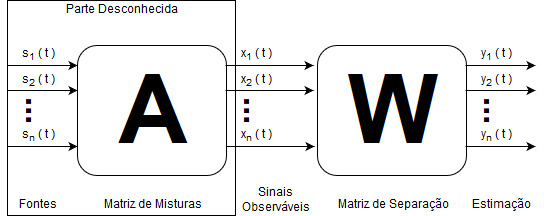
\includegraphics[scale=0.7]{imagens/diagramaBSS.jpg}
    \caption{Diagrama de blocos da ICA}
    \label{fig:DigramaBSS}
    \end{center}
\end{figure}

Existem diversos algoritmos de ICA, sendo que esses podem ser divididos em dois grandes grupos, a saber: os que utilizam Estatísticas de Segunda Ordem (ESO) para estimar ${\bf W}$ e aqueles que utilizam Estatísticas de Ordem Superior (EOS) \cite{faier2011analise}.
Neste trabalho, foram escolhidos dois algoritmos ESO: Algoritmo para Extração de Múltiplos Sinais (AMUSE – \texit{Algorithm for Multiple Unknown Source Extraction} \cite{tong1990amuse})  e Identificação Cega de Segunda Ordem (SOBI – \texit{Second Order Blind Identification} \cite{belouchrani1993second}). Antes de explicar o funcionamento de cada ICA utilizada nesse trabalho, deve-se explicar uma etapa comum a ambas ICAs que é a etapa de braqueamento do sinal.

\section{Branqueamento}

 O braqueamento é uma transformação linear do vetor de sinais observáveis ${\bf x}$ para um vetor branco ${\bf z}$ de tal forma que seus componentes sejam descorrelacionados e com variâncias unitárias. Matematicamente:

\begin{equation}
    E\{{\bf z}*{\bf z}^{T}\}= {\bf I} 
    \label{eq:branco1}
\end{equation}
onde ${\bf I}$ é a matriz indentidade. A transformação linear de ${\bf x}$ em ${\bf z}$ se dá por:

\begin{equation}
    {\bf z}= {\bf V}*{\bf x} 
    \label{eq:branco1}
\end{equation}
onde ${\bf V}$ é a matriz de braqueamento. 

Seja ${\bf E=[e_{1} \quad e_{2}\quad \cdots \quad e_{m}]}$ uma matriz cujas colunas são autovetores de norma unitária da matriz de covariância ${\bf C_{x}}=E\{{\bf x*x}^{T}\}$, e ${\bf D=[d_{1} \quad d_{2} \quad \cdots \quad d_{m}]}$ uma matriz diagonal contendo os autovalores de ${\bf C_{x}}$. Então, pode-se escrever ${\bf V}$ como \cite{hyvarinen2004independent}:

\begin{equation}
    {\bf V}= {\bf E}*{\bf D}^{-1/2}*{\bf E}^{T} 
    \label{eq:branco2}
\end{equation}

Assim, das equações (\ref{eq:branco1}), (\ref{eq:branco2}) e (\ref{eq:ICA2}) tem-se:

\begin{equation}
    {\bf z} = {\bf E*D^{-1/2}*E^{T}*A*s = A_{o}*s}
    \label{eq:branco3}
\end{equation}

Uma característica importante do braqueamento é que a nova matriz $\bf{A_{o}}$ é ortogonal, o que reduz o número de parâmetros a serem estimados posteriormente pela ICA. Outra importância do braqueamento é a aplicação da hipótese de covariâncias diferentes para séries temporais.

\section{Hipótese de covariâncias diferentes}

A hipótese de covariâncias diferentes para séries temporais, significa assumirmos que para cada componente independente, a forma da estrutura temporal é dada pelas covariâncias de cada sinal \cite{faier2011analise}. Assim, após a remoção da média de $x(t)$, tem-se que a matriz de covariância deslocada no tempo vale:

\begin{equation}
   {\bf C_{x}^{\tau}} = E\{{\bf x}(t)*{\bf x}^{T}(t-\tau)\}
    \label{eq:branco4}
\end{equation}

Deve-se então encontrar uma matriz de separação ${\bf W}$ que faça as covariâncias defasadas serem iguais a zero. Um exemplo simples é considerar somente uma matriz de covariância atrasada ($\tau = 1$). Após remover a média e braquear ${\bf x}(t)$, pela equação (\ref{eq:branco3}) tem-se que:

\begin{equation}
   {\bf y}(t) = \left({\bf A_{o}}\right)^{-1} * {\bf z}(t) .: {\bf y}(t) = {\bf W_{o}} * {\bf z}(t)
    \label{eq:branco5}
\end{equation}
\begin{equation}
   {\bf y}(t-\tau) = {\bf W_{o}} * {\bf z}(t-\tau)
    \label{eq:branco6}
\end{equation}
onde ${\bf W_{o}}$ é a matriz de separação ortogonal. Pelas propriedades de linearidade e ortogonalidade, pode-se escrever a matriz dos sinais branqueados como \cite{faier2011analise}: 

\begin{equation}
   \overline{{\bf C_{z}}^{\tau}} =  {\bf W_{o}}^{T}*\overline{{\bf C_{y}}^{\tau}}*{\bf W_{o}}
    \label{eq:branco7}
\end{equation}
onde $\overline{{\bf C_{z}}^{\tau}}=\frac{1}{2}*({\bf C_{z}^{\tau}+(C_{z}^{\tau}})^{T})$. Estendendo esse raciocínio para vários atrasos, é suficiente que apenas uma covariância seja diferente das demais. Assim, a escolha de $\tau$ não seria tão problemática. No entanto, é pouco provável a diagonalização exata, o que leva a formular um indicador para o grau de diagonalização:

\begin{equation}
   off({\bf M}) =  \sum_{i \neq j}m^{2}_{ij}
    \label{eq:branco8}
\end{equation}
onde ${\bf M = \{C_{z}^{1},C_{z}^{2},...,C_{z}^{\tau}\}}$. 

Ambas as ICAs utilizadas neste trabalho utilizam-se da hipótese de covariâncias diferentes para séries temporais para realizar a estimação de $\bf W$

\subsection{AMUSE}

Esta ICA é baseada na decomposição de autovalores de uma simples matriz de covariância atrasada no tempo para dados pré-branqueados. Baseando-se na diagonalização de apenas uma matriz de separação, seu algoritmo pode ser escrito como \cite{faier2011analise}:

 \begin{algorithm}[h]
   \SetAlgoLined
   \Inicio{
   Branqueie os dados de ${\bf x}(t)$ para obter ${\bf z}(t)$ \\
   Calcule a decomposição de autovalores de $\overline{{\bf C_{z}}^{\tau}}=\frac{1}{2}*({\bf C_{z}^{\tau}+(C_{z}^{\tau}})^{T})$ para um dado $\tau$ \\  
   Os autovalores obtidos são as linhas da matriz de separação $\bf{W}$ 
   }
   \Retorna{$\bf{W}$}
   \label{alg1}
   \caption{\textsc{AMUSE}}
 \end{algorithm}

\subsection{SOBI}

A ICA SOBI, assim como a AMUSE, também se baseia na decomposição de autovalores de matrizes de covariância, porém diferentemente da ICA AMUSE, a ICA SOBI utiliza de $p$ matrizes transladas de $\tau$. Com o objetivo de minimizar $off(M)$, tem-se a seguinte função objetivo:

\begin{equation}
   \Im ({\bf W_{o}})  =  \sum_{\tau \in {\bf S}}off(\overline{{\bf C_{y}^{\tau}}})
    \label{eq:sobi1}
\end{equation}
onde $\overline{{\bf C_{y}^{\tau}}}={\bf W_{o}^{T}*\overline{C_{y}^{\tau}}*W_{o}}$, e ${\bf S}$ é o conjunto de atrasos. Pode-se utilizar, por exemplo, um método do gradiente descendente com o seguinte passo \cite{hyvarinen2004independent}:

\begin{equation}
   \Delta ({\bf W_{o}})  =  \sum_{\tau \in {\bf S}}diag ({\bf W_{o}^{T}*\overline{C_{y}^{\tau}}*W_{o}}))^{-1}*{\bf W_{o}*\overline{C_{z}^{\tau}}}
    \label{eq:sobi2}
\end{equation}

Vale destacar que ${\bf W_{o}}$ deve ser ortogonalizado a cada iteração. Assim um possível pseudo algoritmo  é mostrado no Algoritmo 2.

 \begin{algorithm}[h]
   \SetAlgoLined
   \Inicio{
   Branqueie os dados de ${\bf x}(t)$ para obter ${\bf z}(t)$ \\
   Calcule as ${p}$ matrizes de covariância ${\bf C_{z}^{\tau}}$\\
   Calcule ${\bf W_{o}}$ e $\Delta ({\bf W_{o}})$\\
   \Para {$|\Delta ({\bf W_{o})}|> \delta $}
   {
        Atualize ${\bf W_{o}}$\\
        Ortogonalize ${\bf W_{o}}$\\
        Calcule  $|\Delta ({\bf W_{o}})|$
   }
   }
   \Retorna{${\bf W_{o}}$}
   \label{alg2}
   \caption{\textsc{SOBI Gradiente Descendente}}
 \end{algorithm}
 
 Outro possível algoritmo é aplicar sucessivas diagonalizações conjuntas na matriz ${\bf M}$ e na matriz ${\bf A_{o}}$ \cite{belouchrani1993second,belouchrani2000robust}. Para isso, inicialmente define-se a matriz ${\bf G}$:
 
 \begin{equation}
      {\bf G} = \left[
        \begin{array}{c}
            {\bf M}(j,j:m:p*m)-{\bf M}(q,q:m:p*m)  \\
            {\bf M}(j,q:m:p*m)+{\bf M}(q,j:m:p*m)  \\
            i*({\bf M}(q,j:m:p*m)-{\bf M}(j,q:m:p*m))
        \end{array}
        \right]
    \label{eq:sobi3}
\end{equation}
 onde, $j$ e $q$ são contadores e $i$ é o número imaginário equivalente a $\sqrt{(-1)}$.
 
 Após a definição da matriz ${\bf G}$, define-se também a matriz ${\bf G'}=real( {\bf G*G}^{T})$. Em seguida, calcula-se então os autovetores  ${\bf R_{cp}}$ de ${\bf G'}$, bem como a sua matriz diagonal ${\bf D_{cp}}$. Os ângulos da rotação $\alpha_{1}, \alpha_{2}$ e $\alpha_{3}$ serão dados pela coluna em ${\bf R_{cp}}$ que possui o maior autovalor em ${\bf D_{cp}}$, e os coeficientes de rotação são calculados de acordo com (\ref{eq:sobi4}):

\begin{equation}
    \begin{array}{c}
        c=\sqrt{(0.5+\frac{\alpha_{1}}{2})} \\
        sr=0.5*\frac{(\alpha_{2}-j*\alpha_{3})}{c}\\
        sc=0.5*\frac{(\alpha_{2}+j*\alpha_{3})}{c}
    \end{array}
    \label{eq:sobi4}
\end{equation}

Caso o módulo de $sr$ seja maior que um $\delta$ escolhido, deve-se atualizar os valores das matrizes  ${\bf M}$ e ${\bf A_{o}}$ da seguinte maneira:

\begin{equation}
    \begin{array}{c}
    {\bf M}(:,j:m:p*m)=c*{\bf M}(:,j:m:p*m)+sr*{\bf M}(:,q:m:p*m)\\
    {\bf M}(:,q:m:p*m)=c*{\bf M}(:,q:m:p*m)-sc*{\bf M}(:,j:m:p*m)\\
    {\bf M}(j,:)=c*{\bf M}(j,:)+sc*{\bf M}(q,:)\\
    {\bf M}(q,:)=c*{\bf M}(q,:)-sr*{\bf M}(j,:)\\
    {\bf A_{o}}(:,j)=c*{\bf A_{o}}(:,j)+sr*{\bf A_{o}}(:,q)\\
    {\bf A_{o}}(:,q)=c*{\bf A_{o}}(:,q)-sc*{\bf A_{o}}(:,j)
    \end{array}
    \label{eq:sobi5}
\end{equation}

Assim, um pseudo algoritmo pode ser escrito como:

 \begin{algorithm}[h]
   \SetAlgoLined
   \Inicio{
   Branqueie os dados de ${\bf x}(t)$ para obter ${\bf z}(t)$ \\
   Calcule as $p$ matrizes de covariância ${\bf C_{z}}^{\tau}$\\
   Inicialize a Matriz ${\bf M}$ como $[{\bf C_{z}^{1},C_{z}^{2},...,C_{z}^{\tau}}]$ \\
   Inicialize a Matriz ${\bf A_{o}}$ como a ${\bf I_{m}}$\\
   \Para {$|sr|> \delta $}
   {
    \Para{$j = 1$ até $m-1$}
    {
        \Para{$q = j+1$ até $m$}{
            Calcule ${\bf G}$\\
            Calcule ${\bf G'}$\\
            Calcule ${\bf R_{cp}}$ e ${\bf D_{cp}}$\\
            Calcule$[\alpha_{1};\alpha_{2};\alpha_{3}]$\\ 
            Calcule $c,sr$ e $sc$\\
            \Se{$|sr|> \delta $}{
                Atualize as matrizes ${\bf M}$ e ${\bf A_{o}}$\\ 
            }
        }
    }
   }
   ${\bf W_{o} = A_{o}}^{-1}$
   }
   \Retorna{${\bf W_{o}}$}
   \label{alg3}
   \caption{\textsc{SOBI Diagonalização Conjunta}}
 \end{algorithm}
  
 Neste trabalho, foi escolhido utilizar o algoritmo de diagonalização conjunta para a ICA SOBI.
     

 
\chapter{METODOLOGIA PROPOSTA}
\label{ch:mepro}

O problema proposto para este trabalho é a estimação dos componentes harmônicos e inter-harmônicos de forma que o tempo de processamento do algoritmo de estimação não seja maior que o tempo para realizar a aquisição do bloco de sinal a ser processado. Foi proposto o sistema mostrado na Figura \ref{fig:DigramaSistema}, sendo que nesse sistema foi utilizado apenas um sinal de observação, denominado $x(n)$.

\begin{figure}[!htb]
    \begin{center}
    \advance\leftskip-1cm
    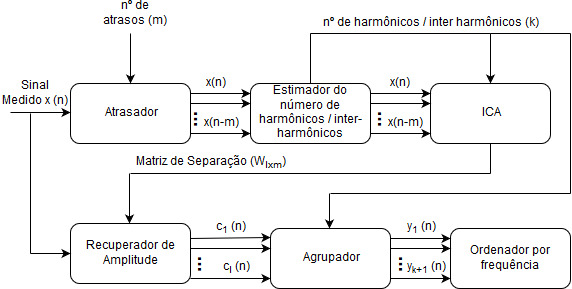
\includegraphics[scale=0.6]{imagens/diagramasitemaproposto.jpg}
    \caption{Diagrama de blocos do sistema proposto}
    \label{fig:DigramaSistema}
    \end{center}
\end{figure}

A seguir, será explicado cada bloco do sistema proposto.

\section{Bloco Atrasador}

Este bloco tem origem no método de geração de múltiplos sinais, chamado \textit{Single Channel ICA} (SCICA), o qual foi proposto por \cite{davies2007source}. O bloco atrasador consiste basicamente em utilizar de sucessivos atrasos aplicados no sinal medido para gerar múltiplos sinais de observação para a ICA, de tal forma que após a aplicação da ICA se tenha:

\begin{equation}
    {{\bf {y}}_{p}}(n)= {\bf W}_{(p,:)}*{\bf{x}}(n)= \sum_{i=0}^{m-1}({\bf W}_{(p,m-i)}*{x}(n-i))
    \label{eq:SCICA}
\end{equation}
onde ${\bf {y}}_{p}(n)$ é a p-ésima fonte separada e ${\bf x}(n)=[x(n), x(n-1),..., x(n-m)]^T$ é o vetor de observação, sendo neste caso composto por amostras transladadas à direita. 

A equação (\ref{eq:SCICA}) implica que: cada linha da matriz de separação ${\bf W}$ contém os coeficientes de resposta ao impulso de um filtro FIR (\textit{Finite-duration Impulse Response}) e que as ICAs só serão capazes de separar e identificar corretamente as fontes caso estas não apresentem sobreposição espectral \cite{limanova}.

Na Figura \ref{fig:DigramaSistema}, pode-se observar que o bloco atrasador tem como entradas o sinal medido $x(n)$ e o número de atrasos sucessivos $m$ a ser aplicado. Pode-se perceber também que sua saída é o conjunto de $m$ amostras \{$x(n), x(n-1),..., x(n-m)$\}. Supondo que o comprimento de $x(n)$ medido antes do bloco atrasador seja $N$, então o comprimento de ${\bf x}(n)$ após o bloco atrasador deve ser $(N-m)$. 

\section{Bloco Estimador do número de harmônicos/inter-harmônicos}

Sabe-se que as fontes são dadas de forma que:
 
\begin{equation}
    {s}_{i}(n)=Vm_{i}*\sin(\omega_{i}*n*T_S+\phi_{i})
    \label{eq:SinalEstimacao1}
\end{equation}
onde ${\bf s}_{i}(n)$ representa uma fonte qualquer, $Vm_{i}$ é a amplitude dessa fonte, $\phi_{i}$ é a fase inicial desta fonte, $\omega_{i}$ é a frequência em rad/s e $T_s$ é o período de amostragem.

Assim o sinal observável pode ser escrito como:

\begin{equation}
     x(n)=\sum_{i=1}^{K}(a_{i}*Vm_{i}*\sin(\omega_{i}*n*T_s+\phi_{i}))
    \label{eq:SinalEstimacao0}
\end{equation}
onde $x(n)$ representa o sinal observável,  $a_{i}$ é o ganho de mistura da fonte $i$ para o sinal observável e $K$ é o número real de fontes.

Para estimar o número de harmônicos e inter-harmônicos $K$, foi utilizado o algoritmo \textit{Exact Model Order} (EMO), proposto por \cite{jain2012exact}. Esse algoritmo tem sua base na curva de densidade espectral de potência do sinal de entrada.

Inicialmente, são calculados os autovalores ($\lambda_i$)  da matriz de autocorrelação (${\bf R_{x}}$) do sinal de entrada $x(n)$. Então, calcula-se a diferença relativa de sucessivos autovalores (${\bf RD}$), dada por:

\begin{equation}
    {\bf RD} = \frac{\lambda_{i}-\lambda_{(i-1)}}{\lambda_{(i-1)}} .:\forall i=2,3,...,m
    \label{eq:EMO}
\end{equation}
onde $\lambda_{i}$ é o i-ésimo autovalor de ${\bf R}_{x}$, $m$ é o tamanho de ${\bf R}_{x}$ e o índice $i$ é denominado Índice de Diferença Relativa (${\bf RDI}$). 

Este cálculo acentua o limite entre o subespaço de sinal e o subespaço de ruído, pois normalmente o primeiro ou o segundo "pico" de amplitude de ${\bf RD}$ corresponde à fronteira entre o último autovalor do subespaço de sinal e o primeiro autovalor do subespaço de ruído.

Para uma melhor estimativa, são escolhidos empiricamente os 5 primeiros "picos" de amplitude de ${\bf RD}$, onde inicialmente o ${\bf RDI}$ do "pico" de ${\bf RD}$ mais distante da origem é escolhido como estimativa inicial da ordem do modelo($j$). Então, para validar essa estimativa, é verificado se

\begin{equation}
    \lambda_{j} \geq \alpha*\frac{\lambda_{j+1}+\lambda_{j+2}+...+\lambda_{m}}{m-j}
    \label{eq:EMO1}
\end{equation}
onde $\lambda_{j}$ é o autovalor relativo ao ${\bf RDI}$ selecionado e $\alpha$ é o fator de sensibilidade, também escolhido empiricamente.

Caso não ocorra a validação, é escolhido o ${\bf RDI}$ do segundo "pico" de ${\bf RD}$ mais distante da origem, e assim sucessivamente, até encontrar algum valor de $\lambda_{j}$ que satisfaça a inequação (\ref{eq:EMO1}). A ordem do modelo, ou seja, o número de harmônicos/inter-harmônicos a serem estimados ($k$), será:

\begin{equation}
    k=\frac{j}{2}
    \label{eq:EMO2}
\end{equation}

O Bloco estimador do número de harmônicos/inter-harmônicos possui como entrada o conjunto de $m$ sinais atrasados, e sua saída é o número de harmônicos/inter-harmônicos $k$, o qual servirá de controle para o Bloco da ICA e o para o Bloco de Agrupamento, a serem explicados a seguir.

\section{Bloco ICA }

O Bloco ICA possui como parâmetros de entrada os $m$ sinais atrasados e o número de harmônicos/inter-harmônicos $k$. 
Tem-se que a equação (\ref{eq:SinalEstimacao1}) pode ser reescrita da seguinte forma:

\begin{equation}
    {s}_{i}(n)= Vm_{i}*\sin(\omega_{i}*n*T_s)*\cos(\phi_{i})+Vm_{i}*\cos(\omega_{i}*n*T_s)*\sin(\phi_{i})
    \label{eq:SinalEstimacao2}
\end{equation}

Desta forma, cada fonte ${s}_{i}(n)$ é formada por dois componentes perpendiculares entre si. Assim, para cada fonte $i$, a ICA deve estimar dois componentes, resultando em um número de estimativas de no mínimo $2*k$ componentes independentes. As ICAs possuem como características a não recuperação dos ganhos \{$Vm_{i}$\}, sendo também necessária uma etapa de recuperação de amplitude. Tal etapa será descrita logo a seguir.

As técnicas de ICA já foram explicadas no capitulo \ref{ch:ica}. No presente capítulo, cabe explicar como elas foram utilizadas bem como as modificações implementadas neste trabalho.

A modificação implementada na ICA SOBI foi um controle do número de iterações que o algoritmo usa para estimar a matriz de separação ${\bf W}$, mostrada no Algoritmo 3 do Capítulo \ref{ch:ica}. Foram substituídos os valores finais das variáveis de controle $j$ (linha 7 do algoritmo) e $q$ (linha 8 do algoritmo) dos laços de repetição. Tais valores foram substituídos de $m$ (número de sinais observáveis) para $2*k$ (dobro do número de harmônicos/inter-harmônicos estimado pelo algoritmo EMO). Também foi implementada uma modificação na ICA AMUSE, para que ela opere no sub-espaço de sinal, ou seja, sua matriz de separação deixou de possuir dimensão $m\times m$ e passou a possuir dimensão $2k\times m$, reduzindo assim a dimensão do problema.

A Figura \ref{fig:amusesobi} mostra a combinação das duas ICAs, na qual destaca-se que a matriz de separação final é dada pelo produto da matriz de separação da ICA SOBI (${\bf W}_{2k\times 2k}$) com a matriz de separação da ICA AMUSE (${\bf W}_{2k\times m}$).

\begin{figure}[!htb]
    \begin{center}
    %\advance\leftskip-1.5cm
    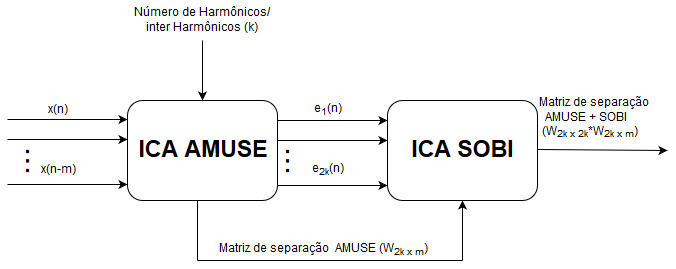
\includegraphics[scale=0.6]{imagens/amuseesobi.jpg}
    \caption{Diagrama de blocos da Combinação de ICAs}
    \label{fig:amusesobi}
    \end{center}
\end{figure}

\section{Bloco Recuperação de Amplitude}

Como já dito anteriormente, a ICA não recupera os ganhos da escala das fontes estimadas. Portanto, se faz necessária a utilização de algum mecanismo para mapear os sinais separados de volta para o domínio original dos sinais observados.
Em uma aplicação padrão da ICA, pode-se mapear os sinais separados de volta ao domínio dos sinais de observação por meio de um par de transformações de mistura e separação \cite{davies2007source}. Para sinais temporais, tem-se que:

\begin{equation}
    {\bf y}_{s}^{p}(n)= {\bf A}_{(:,p)}*{\bf W}_{(p,:)}*{\bf x}(n),
    \label{eq:amplitude1}
\end{equation}
onde cada linha da matriz \textbf{${\bf y}_{s}^{p}(n)$} representa o peso original do p-ésimo sinal separado no m-ésimo sinal de observação no instante $n$. Substituindo (\ref{eq:SCICA}) em (\ref{eq:amplitude1}), tem-se que:

\begin{equation}
    {\bf y}_{s}^{p}(n)= {\bf A}_{(:,p)}*\sum_{i=0}^{m-1}({\bf W}_{(p,m-i)}*{\bf x}(n-i)).
    \label{eq:amplitude2}
\end{equation}

Como os sinais observáveis são versões transladadas do sinal medido, pode-se deduzir que o peso da p-ésima fonte estimada seria o mesmo para os $m$ sinais de observação. Entretanto, as estimativas das fontes reconstruídas dependem do alinhamento de cada sinal de observação com o sinal medido. Para obter uma completa invariância à translação do sinal medido, foi implementada a técnica cycle-spinning \cite{coifman1995translation}. Assim, para cada linha $m$ do vetor ${\bf y}_{s}^{p}(n)$, tem-se que:

\begin{equation}
    {\bf c}_{p}(n)= \frac{1}{m}*\sum_{j=0}^{m-1} ({\bf A}_{(j+1,p)}*\sum_{i=0}^{m-1}({\bf W}_{(p,m-i)}*{\bf x}(n-i-j))),
    \label{eq:amplitude3}
\end{equation}

\begin{equation}
    {\bf c}_{p}(n)(n)= \frac{1}{m}*{\bf a}_{p}(n)*{\bf w}_{p}(-n)*{\bf x}(n),
    \label{eq:amplitude4}
\end{equation}
onde ${\bf a}_{p}(n)$ representa o filtro FIR associado ao vetor coluna ${\bf A}_{(:,p)}$. Observa-se que as estimativas ${\bf c}_{p}$ são versões filtradas de ${\bf }x(n)$. Pode-se dizer então que o bloco Recuperador de Amplitude atua como um banco de filtros adaptativos e que sua saída é dada pelas fontes estimadas pela ICA com amplitudes recuperadas. 

\section{Bloco Agrupador e Bloco Ordenador por frequência}

Tem-se pela equação (\ref{eq:SinalEstimacao2}) que cada fonte original é composta por um par de senoides perpendiculares entre si. Pode se dizer então que cada fonte é formada por dois sinais pertencentes a um conjunto $c(n)$.

Existem diversas maneiras de escolher quais pares de sinais devem ser somados para compor uma fonte. Neste trabalho, foi escolhido realizar a Transformada Rápida de Fourier Discreta (DFFT - Discrete Fast Fourier Transform) para analisar o espalhamento espectral de energia de cada sinal estimado. Então, as $2*k$ estimativas de componentes independentes contendo os  maiores valores de energia são agrupadas em $k$ conjuntos de acordo com o seu espalhamento espectral. 

Devido ao fato da associação ser por maior energia e não por frequência, foi necessário utilizar um bloco de Ordenação por frequência para que a saída esteja organizada, bem como para estimar as frequências de cada sinal estimado. Para tal, utiliza-se do algoritmo \textit{zero crossing} \cite{hummel1984zero}. As estimativas restantes, ou seja, aquelas que não possuem as $2*k$ maiores energias, são somadas e consideradas como sinal de ruído, sendo categorizadas como pertencentes ao sub-espaço de ruído. Assim, a saída do bloco Ordenador por frequência deve possuir tamanho igual a $k+1$, onde o último sinal é a estimativa de ruído. 


\chapter{SIMULAÇÃO E RESULTADOS}
\label{ch:simres}

Nesta seção, serão apresentados alguns resultados obtidos pelo método proposto neste trabalho para estimação de harmônicos e inter-harmônicos baseado na ICA. Em especial, será realizada uma série de comparações de eficiência dos algoritmos de ICA para aplicação do método em distintos conjuntos de sinais de teste. Foi utilizado o \textit{software} Matlab para as simulações, pois sua natureza matricial e sua vasta biblioteca de funções facilitaram o desenvolvido de algoritmos que realizavam testes automáticos. Os algoritmos de ICA utilizados foram:

\begin{itemize}
    \item ICA SOBI: algoritmo SOBI por diagonalização conjunta (algoritmo 3 do capítulo \ref{ch:ica}).
    \item ICA SOBI modificada: algoritmo SOBI por diagonalização conjunta e com controle do número de iterações baseado na estimativa do número de componentes senoidais estimado pelo algoritmo EMO.
    \item ICA AMUSE: algoritmo 1 do capítulo \ref{ch:ica}.
    \item Combinação AMUSE e SOBI: combinação na qual aplica-se inicialmente a ICA AMUSE nos sinais de saída do bloco atrasador e em seguida aplica-se a ICA SOBI modificada nos sinais de saída da ICA AMUSE. A matriz de separação resultante é dada pelo produto das matrizes de separação estimadas pelo AMUSE e pelo SOBI (\texit{vide} Figura \ref{fig:amusesobi}).  
\end{itemize}

A fim de exemplificar o que faz cada teste, tem-se a Figura \ref{fig:exemplo}. Nela, pode-se ver que é estimado também o ruído e que a estimação dos componentes senoidais aproxima-se muito dos componentes do sinal real. No primeiro gráfico, tem-se o sinal que deverá ter suas componentes estimadas; nos outros gráficos, exceto o do ruído, tem-se as componentes senoidais que compõem esse sinal, sendo as estimativas obtidas pelo método completo (\texit{vide} Figura \ref{fig:DigramaSistema}) mostradas por linhas tracejadas.

\begin{figure}[!htb]
    \begin{center}
    \advance\leftskip-2.5cm
    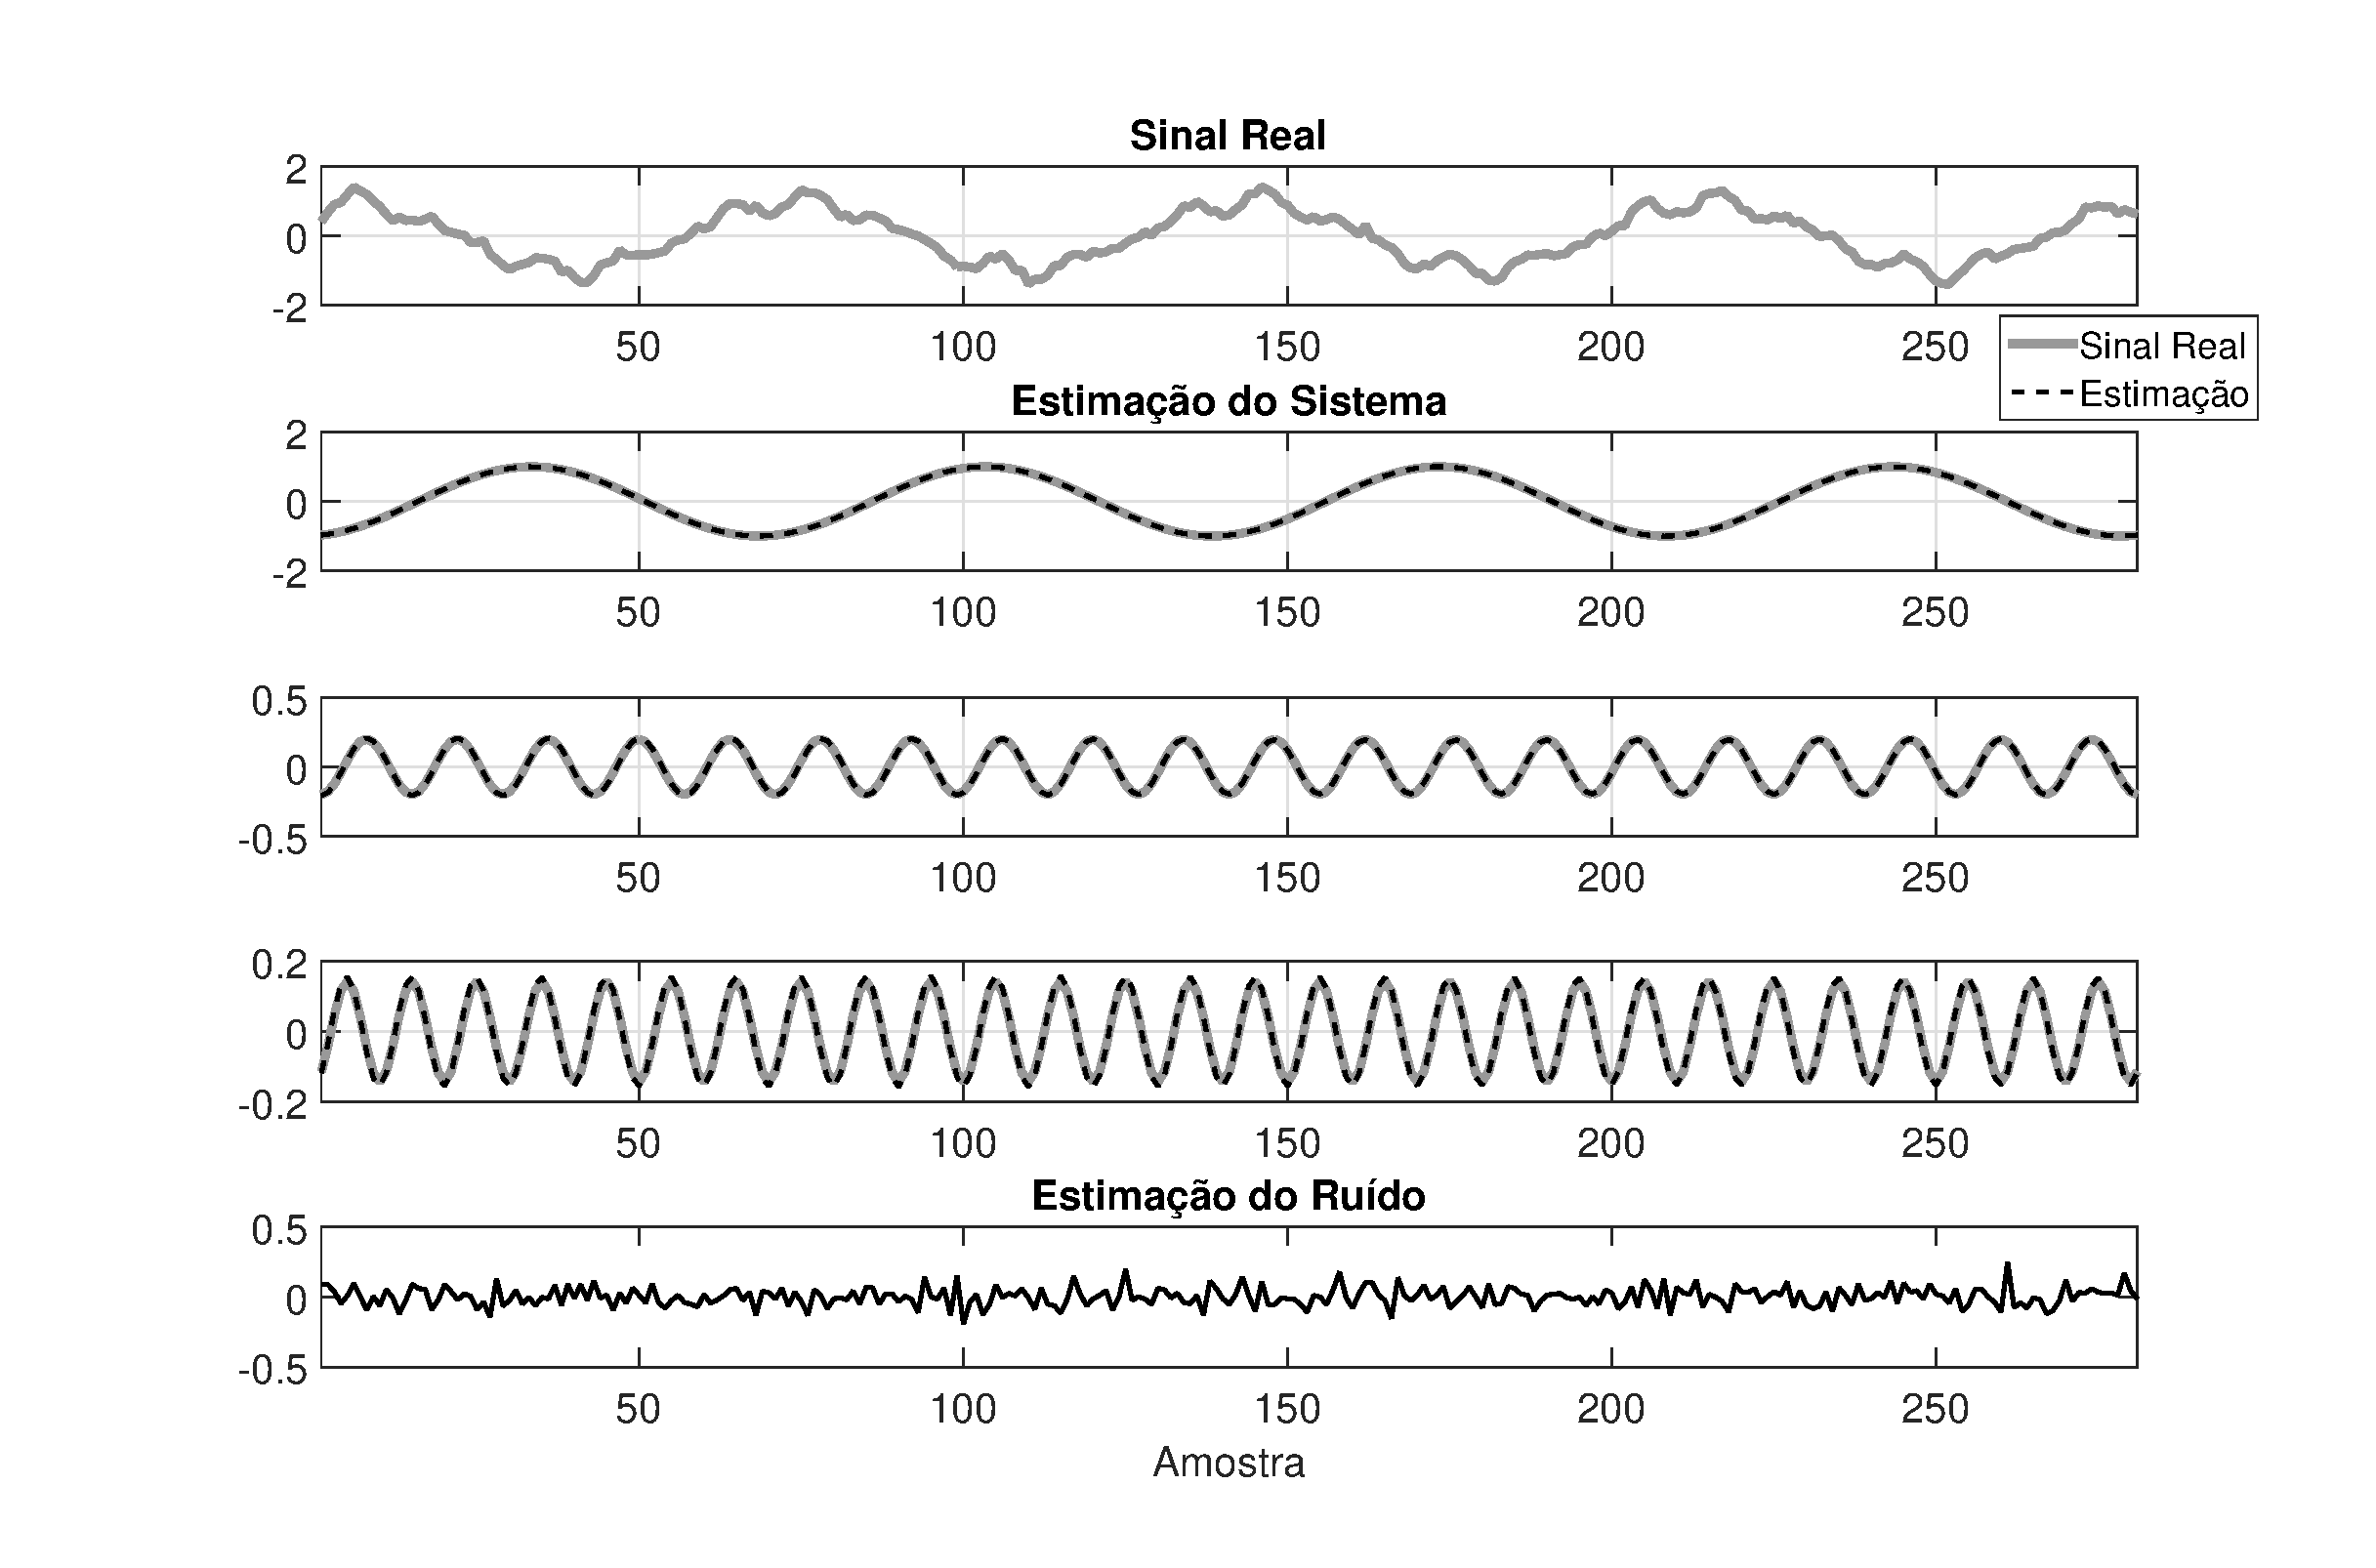
\includegraphics[scale=0.50]{imagens/Exemplov2.eps}
    \caption{Exemplo de estimação obtida pelo método proposto.}
    \label{fig:exemplo}
    \end{center}
\end{figure}

Vale ressaltar que sempre é medido o Tempo de Processamento ($TP$) total do sistema. Além disso, é calculado o Erro Quadrático Médio normalizado ($RMSE$) entre componentes originais e estimativas, e o Tempo de Obtenção ($TO$) do bloco de sinal analisado. O $TO$ diz respeito ao tempo de aquisição do bloco de sinal com base na frequência de amostragem do mesmo. O $RMSE$ e o $TO$ são definidos pelas equações (\ref{eq:RMSE}) e (\ref{eq:TO}), respectivamente:

\begin{equation}
    RMSE = \frac{\sqrt{\frac{\sum_{n=0}^{M} (S(n)-Y(n))^2}{M}}}{\sqrt{\frac{\sum_{n=0}^{M} (S(n))^2}{M}}},
    \label{eq:RMSE}
\end{equation}
onde ${S}(n)$ é o valor real da fonte e ${Y}(n)$ é o valor da estimativa.

\begin{equation}
    TO = \frac{N_s}{F_s},
    \label{eq:TO}
\end{equation}
onde $N_s$ é o número de amostras do sinal e $F_s$ é a sua frequência de amostragem. Deve-se enfatizar que o $RMSE$ é calculado após a remoção do período transitório da filtragem.

\section{Testes Sucessivos}
\label{ch:testesus}

Inicialmente foi testado o método para cada ICA, empregado em um sinal composto por uma combinação aleatória de harmônicos e inter-harmônicos. Para a geração do sinal, utilizou-se uma frequência de amostragem igual a 3.5kHz ($F_s$) e um número de amostras($N_s$) igual a 480. O sinal possui componente fundamental com amplitude de 1V e frequência de 50Hz, o qual foi combinado com 3 (três) inter-harmônicos ou harmônicos aleatórios em amplitude e em frequência. O $TO$ deste sinal foi de $0.1371s$. Houve 100 sorteios de amplitude e frequência, sendo que para cada um foram sorteadas 5 fases. Manteve-se o número de atrasos ($m$) igual a 100 e a relação sinal ruído igual a 30dB (SNRdb = 30). Foi calculado o $\overline{RMSE}$ e o seu desvio padrão ($\sigma$), em porcentagem, através das seguintes equações:

\begin{equation}
    \overline{RMSE} = \frac {\sum_{i=0}^{N_1} RMSE(i) }{N_1}
    \label{eq:RMSEmedio}
\end{equation}
\begin{equation}
    \sigma(\overline{RMSE}) = \frac{\sqrt{\sum_{i=0}^{N_1} (RMSE(i)-\overline{RMSE})^2}}{N_1*\overline{RMSE}} 
    \label{eq:RMSEdesvio}
\end{equation}
onde $i$ é o número do teste e $N_1$ é o número total de testes realizados.

A  Tabela \ref{tab:sorteio} apresenta a forma com que a amplitude e a frequência foram sorteadas. A variável ``rdn'' representa uma variável aleatória com distribuição gaussiana de média zero e variância igual a 1.  

\begin{table}[h]
    \begin{center}
    \caption{Valores sorteados de amplitude e frequência.}
        \begin{tabular}{c|l|l| l}
        \hline
        Componentes & 2 & 3 & 4\\ \hline
        Amplitude   & 1/3 + 2/30*rdn & 1/5 + 2/50*rdn & 1/7 + 2/70*rdn\\ \hline
        Frequência  & 150 + 50*rdn & 250 + 50*rdn & 350 + 50*rdn \\ \hline
        \end{tabular}
        \label{tab:sorteio}
    \end{center}
    
\end{table}

A Tabela \ref{tab:SinSimRMSETP} mostra o Erro Quadrático Médio ($\overline{RMSE}$) bem como seu desvio padrão. Além disso, apresenta o Tempo Processamento médio ($\overline{TP}$), bem como o tempo máximo($T_{max}$) e o tempo mínimo($T_{min}$) de cada método. Pode-se perceber que a ICA SOBI apresenta o maior $\overline{TP}$, e ao comparar essa com a ICA SOBI modificada, nota-se que a ICA SOBI modificada apresenta um $\overline{TP}$ muito menor que a ICA SOBI, para um $\overline{RMSE}$ ainda um pouco menor. Também é possível notar que a ICA AMUSE é a ICA com o menor $\overline{TP}$, apresentando também um $\overline{RMSE}$ baixo, porém o mais elevado dos testes. Vale destacar que a combinação das ICAs SOBI modificada e AMUSE possui um $\overline{RMSE}$ menor que qualquer outra ICA, e que todas as ICAs, exceto a ICA SOBI sem modificação, realizam a estimação em um tempo médio menor que o $TO$ do sinal ($TO=0.1371~s$). A ICA SOBI modificada e a Combinação são as únicas que realizam o processamento em um tempo máximo ($T_{max}$) menor que o $TO$.

\begin{table}[h]
    \begin{center}
    \caption{Valores médios do Erro Quadrático Médio (RMSE) e do Tempo de Processamento(TP) para um sinal com quatro componentes.}
        \begin{tabular}{c|c c c c}
        \hline
        \textbf{ICA} & \textbf{SOBI} & \textbf{SOBI mod} & \textbf{AMUSE} & \textbf{Combinação}\\ \hline
        $\overline{RMSE}$   & 0.19 $\pm$ 7.5\% & 0.17 $\pm$ 7.9\% & 0.21 $\pm$ 6.3\% & 0.16 $\pm$ 8\%\\ \hline
        $\overline{TP}$    & 9.51s   & 0.037s   & 0.014s   & 0.020s  \\ \hline
        $T_{max}$             & 34.61s  & 0.047s   & 0.271s   & 0.028s  \\ \hline
        $T_{min}$             & 4.82s   & 0.031s   & 0.012s   & 0.016s  \\ \hline
        \end{tabular}
        \label{tab:SinSimRMSETP}
    \end{center}
    
\end{table}

Na Tabela \ref{tab:SinSimTPBlock}, é mostrada a quantidade do tempo de processamento total que é demandada por cada bloco, em média. As siglas na tabela dizem respeito aos tempos de processamento dos seguintes blocos: $\overline{BIC}$: Bloco da ICA; $\overline{EMO}$: Bloco de estimação do número de harmônicos e inter-harmônicos; $\overline{CCS}$: Bloco de recuperação de amplitude; $\overline{FFT}$: Bloco de Agrupamento e; $\overline{ORD}$: Bloco de Ordenação por Frequência. 

Analisando-se a Tabela \ref{tab:SinSimTPBlock}, nota-se que no método que emprega a ICA SOBI original, o $\overline{BIC}$ é o responsável absoluto pela maior parte do $\overline{TP}$ do método. Com isto, pode-se dizer que a responsabilidade da demora do método é basicamente inteira do próprio algoritmo da ICA. Também é importante notar que o $\overline{ORD}$ tem boa parcela no tempo total para quase todas as ICAs, exceto para a ICA SOBI. Como o bloco correspondente é apenas para ordenar as estimativas por frequências, o mesmo pode ser desligado dependendo da aplicação. Vale destacar que o $\overline{EMO}$ é pouco influente no tempo final de processamento do método para todas as ICAs. Por fim, o $\overline{FFT}$ também demanda boa parte do tempo para quase todas as ICAs, significando que outras estratégias de agrupamento, além da DFFT, devem ser investigadas em trabalhos futuros.  

\begin{table}[!htb]
    \begin{center}
        \caption{Tempo de Processamento médio por bloco, em porcentagem, para um sinal com quatro componentes.}
        \begin{tabular}{c|c c c c c}
        \hline
        \textbf{ICA}          & $\overline{BIC}$ (\%)  & $\overline{EMO}$(\%) & $\overline{CCS}$(\%)   & $\overline{FFT}$(\%)  & $\overline{ORD}$(\%)\\ \hline
        \textbf{SOBI}        & 99.8      & \ll 1     & \ll 1       & \ll 1      & \ll 1     \\ \hline
        \textbf{SOBI mod}     & 44.5        & 3.5     & 19.6        & 20.3       & 11.2     \\ \hline
        \textbf{AMUSE}        & 21.3        & 9.6      & 4.7       & 35.2       & 26.9     \\ \hline
        \textbf{Combinação}   & 48.7        & 5.9     & 3.0       & 23.2       & 17.6     \\ \hline
        \end{tabular}
        \label{tab:SinSimTPBlock}
    \end{center}
\end{table}

Após testar os métodos com o sinal com quatro componentes, foi realizado um novo teste com sinais de composição com mais componentes. Neste teste, a amplitude da componente fundamental foi fixada em 25V, sendo que essa foi combinada com 7 componentes harmônicos ou inter-harmônicos decididos aleatoriamente, havendo também diminuição da frequência de amostragem para 2.4kHz, o que corresponde a um $TO$ de $0.2s$ para a mesma quantidade de amostras do sinal do primeiro teste ($N_s=480$) e mesma relação sinal ruído (SNRdb = 30). A  Tabela \ref{tab:sorteioc} apresenta a forma com que as amplitudes e as frequências foram sorteadas. A Tabela \ref{tab:SinComRMSETP} apresenta os resultados para este teste.  

\begin{table}[h]
\advance\leftskip -1.5cm
    \begin{center}
    \caption{Valores sorteados de amplitude e frequência.}
        \begin{tabular}{c|m{1.5cm}|m{1.5cm}|m{1.5cm}|m{1.3cm}|m{1.5cm}|m{1.5cm}|m{1.5cm}}
        \hline
        Componentes &  2 & 3 & 4 & 5 & 6 & 7 & 8\\ \hline
        Amplitude   &  3 + 0.6*rdn & 0.5 + 0.1*rdn & 3 + 0.6*rdn & 5 + rdn & 1 + 0.2*rdn & 4 + 0.8*rdn & 2.5 + 0.5*rdn\\ \hline
        Frequência  & 100 + 15*rdn & 150 + 15*rdn & 250 + 25*rdn & 350 + 25*rdn & 450 + 25*rdn & 550 + 25*rdn & 650 + 25*rdn \\ \hline
        \end{tabular}
        \label{tab:sorteioc}
    \end{center}
\end{table}

\begin{table}[h]
    \begin{center}
    \caption{Valores médios do Erro Quadrático Médio (RMSE) e do Tempo de Processamento(TP) para um sinal com oito componentes.}
        \begin{tabular}{c|c c c c}
        \hline
        \textbf{ICA} & \textbf{SOBI} & \textbf{SOBI mod} & \textbf{AMUSE} & \textbf{Combinação}\\ \hline
        $\overline{RMSE}$   & 0.38 $\pm$ 8.1\% & 0.09 $\pm$ 12.7\% & 0.40 $\pm$ 6.3\% & 0.08 $\pm$ 11.4\%\\ \hline
        $\overline{TP}$    & 8.34s   & 0.063s   & 0.020s   & 0.049s  \\ \hline
        $Tmax$             & 28.08s  & 0.073s   & 0.046s   & 0.065s  \\ \hline
        $Tmin$             & 4.49s   & 0.054s   & 0.018s   & 0.038s  \\ \hline
        \end{tabular}
        \label{tab:SinComRMSETP}
    \end{center}
\end{table}

Ao analisar a Tabela \ref{tab:SinComRMSETP}, pode-se concluir que as ICAs SOBI e AMUSE não possuem bom desempenho quando comparadas com a ICA SOBI modificada e com a Combinação de ICAs, já que as duas primeiras possuem um alto $\overline{RMSE}$ e a ICA SOBI ainda apresenta um alto $\overline{TP}$. Assim, pode-se concluir que as modificações feitas na ICA SOBI melhoraram a resposta significativamente, seja em seu $\overline{TP}$ ou em seu $\overline{RMSE}$. Também deve-se enfatizar que a Combinação de ICAs possui um $\overline{RMSE}$ comparável ao da ICA SOBI modificada, porém apresentou um $\overline{TP}$ significativamente menor. Também vale destacar que, novamente, todas as ICAs, exceto a ICA SOBI sem modificações, apresentaram $TP$ menor que o $TO$, mesmo para um sinal mais complexo. Comparando a Tabela \ref{tab:SinComRMSETP}  com a Tabela \ref{tab:SinSimRMSETP}, parecebe-se que há um aumento significativo no $\sigma(\overline{RMSE})$ para todas as ICAs, exceto para a ICA AMUSE.

Realizando a comparação da Tabela \ref{tab:SinComTPBlock} com a Tabela \ref{tab:SinSimTPBlock}, pode-se notar que a ICA SOBI permanece inalterada em termos de tempo de processamento médio percentual. Entretanto, houve um grande aumento no $\overline{BIC}$ para a ICA SOBI modificada e para a Combinação das ICAs AMUSE e SOBI. Tal resultado mostra que a complexidade do sinal aumenta o tempo necessário para a estimação por parte do bloco de ICA. O mesmo não ocorreu com a ICA AMUSE, pois essa ainda apresentou uma redução no $\overline{BIC}$, ocorrendo um aumento principalmente em $\overline{ORD}$. Isto se deve provavelmente à própria complexidade maior do sinal.

\begin{table}[!htb]
    \begin{center}
        \caption{Tempo de Processamento médio por bloco em porcentagem para um sinal com oito componentes.}
        \begin{tabular}{c|c c c c c}
        \hline
        \textbf{ICA} & $\overline{BIC}$ (\%)  & $\overline{EMO}$(\%) & $\overline{CCS}$(\%)   & $\overline{FFT}$(\%)  & $\overline{ORD}$(\%)\\ \hline
        \textbf{SOBI }        & 99.6      & \ll 1     & \ll 1       & \ll 1      & \ll 1     \\ \hline
        \textbf{SOBI mod}     & 58.5        & 2.0     & 11.6        & 15.3       & 12.1     \\ \hline
        \textbf{AMUSE}        & 16.1        & 6.3     & 5.9       & 35.1       & 36.0     \\ \hline
        \textbf{Combinação}   & 65.3        & 2.4     & 2.4       & 14.4       & 14.8     \\ \hline
        \end{tabular}
        \label{tab:SinComTPBlock}
    \end{center}
\end{table}

Por fim, pode-se concluir novamente que as ICAs SOBI original e AMUSE possuem um desempenho bem inferior às ICAs propostas neste trabalho. Então, para os próximos testes será escolhido utilizar apenas as ICA SOBI modificada e a combinação da ICA AMUSE e a ICA SOBI modificada.

Com a finalidade de testar o sistema tanto em relação à sua sensibilidade ao número de atrasos quanto ao ruído do sinal de entrada, será escolhido um grupo de sinais distintos para a realização dos ensaios. Os parâmetros desses sinais podem ser vistos na Tabela \ref{tab:Sinais}, os quais foram obtidos em \cite{jain2012exact}, \cite{he2015separation} e \cite{liu2016resolution}. A exceção é para o Sinal 1 ($S1$), que é  um seguimento da série de Fourier de uma onda quadrada. Os valores de $F_s$ e $N_s$ correspondem à frequência de amostragem e ao tamanho do sinal, respectivamente.

\begin{table}[!htb]
    \begin{center}

        \caption{Sinais Escolhidos para os ensaios.}
        \begin{tabular}{c| m{4cm} | m{4cm} |c|c|c}
        \hline
        Sinais & Amplitude (V) & Frequência (Hz) & $F_s$ (kHz) & $N_s$ & $TO$ (s)\\\hline
        Sinal 1 (S1)& 1 1/5 1/7 1/11  & 50 250 350 550  & 3.5 & 480 & 0.13\\ \hline
        Sinal 2 (S2)& 25  3  0.5  3  5  1  4  2.5 & 50  82  100  150  182  200  250  350 & 2.4 & 480 & 0.20 \\ \hline
        Sinal 3 (S3)& 30  380  20  45  152 & 40  50 80  175  250  & 1.0 & 1000 & 1.00\\ \hline
        Sinal 4 (S4)& 1.8  3.1  0.9  0.3  0.1  0.16  0.13  0.1 & 16.4  50  83.7  116.1  150  183.2  216.3  250 & 5.0 & 1000 & 0.20\\ \hline
        Sinal 5 (S5)& 1  0.1  0.6  0.35  0.08  0.2  & 50  125  250  412  550  & 2.0 & 400 & 0.20\\ \hline
        \end{tabular}
        \label{tab:Sinais}
    \end{center}
\end{table}

\section{Sensibilidade ao Número de Atrasos}
Neste teste foram sorteadas 100 fases aleatórias para cada componente de frequência da Tabela \ref{tab:Sinais} e, com o intuito de automatizar a variação do número de atrasos ($m$) do bloco Atrasador (\texit{vide} Figura \ref{fig:DigramaSistema}), foi escolhido variá-lo em um intervalo desde apenas o número de amostras em um ciclo da componente fundamental ($F_s$/50) até o maior valor possível para o qual ainda haveria estimação das fontes ($N_s$/3). A relação sinal ruido em decibéis (SNRdb) foi mantida em 100~dB, pois o objetivo deste teste foi analisar o comportamento do sistema dado uma grande variação no número de atrasos.
Em cada gráfico, o eixo azul (à esquerda) representará a amplitude do $\overline{RMSE}$ das 100 fases sorteadas, enquanto que o eixo vermelho (à direita) representará o $\overline{TP}$ das 100 fases sorteadas. Vale também destacar que em cada figura, o gráfico superior corresponde ao sistema com a ICA SOBI modificada, enquanto que o gráfico inferior corresponde ao sistema com a combinação de ICAs AMUSE e SOBI modificada. 

Na Figura \ref{fig:atrasoS1}, pode-se notar que a amplitude do $\overline{RMSE}$ de ambos os gráficos possui um comportamento parecido, sendo que quando o número de atrasos é maior que 103, o sistema começa a ter uma resposta pior, e a partir de $m=135$, a amplitude do $\overline{RMSE}$ se torna muito mais elevada do que quando $m$ é baixo. Também pode-se destacar que a variação do $\overline{TP}$ em função da variação do número de atrasos foi muito menor para o método empregando a Combinação de ICAs do que para o método empregando a ICA Sobi Modificada. Além disso, percebe-se que para ambas as ICAs, o tempo de processamento foi menor que o tempo de obtenção do sinal ($TO=0.13$s) para todos os valores de atraso.

\begin{figure}[!htb]
    \begin{center}
    \advance\leftskip -1.5cm
    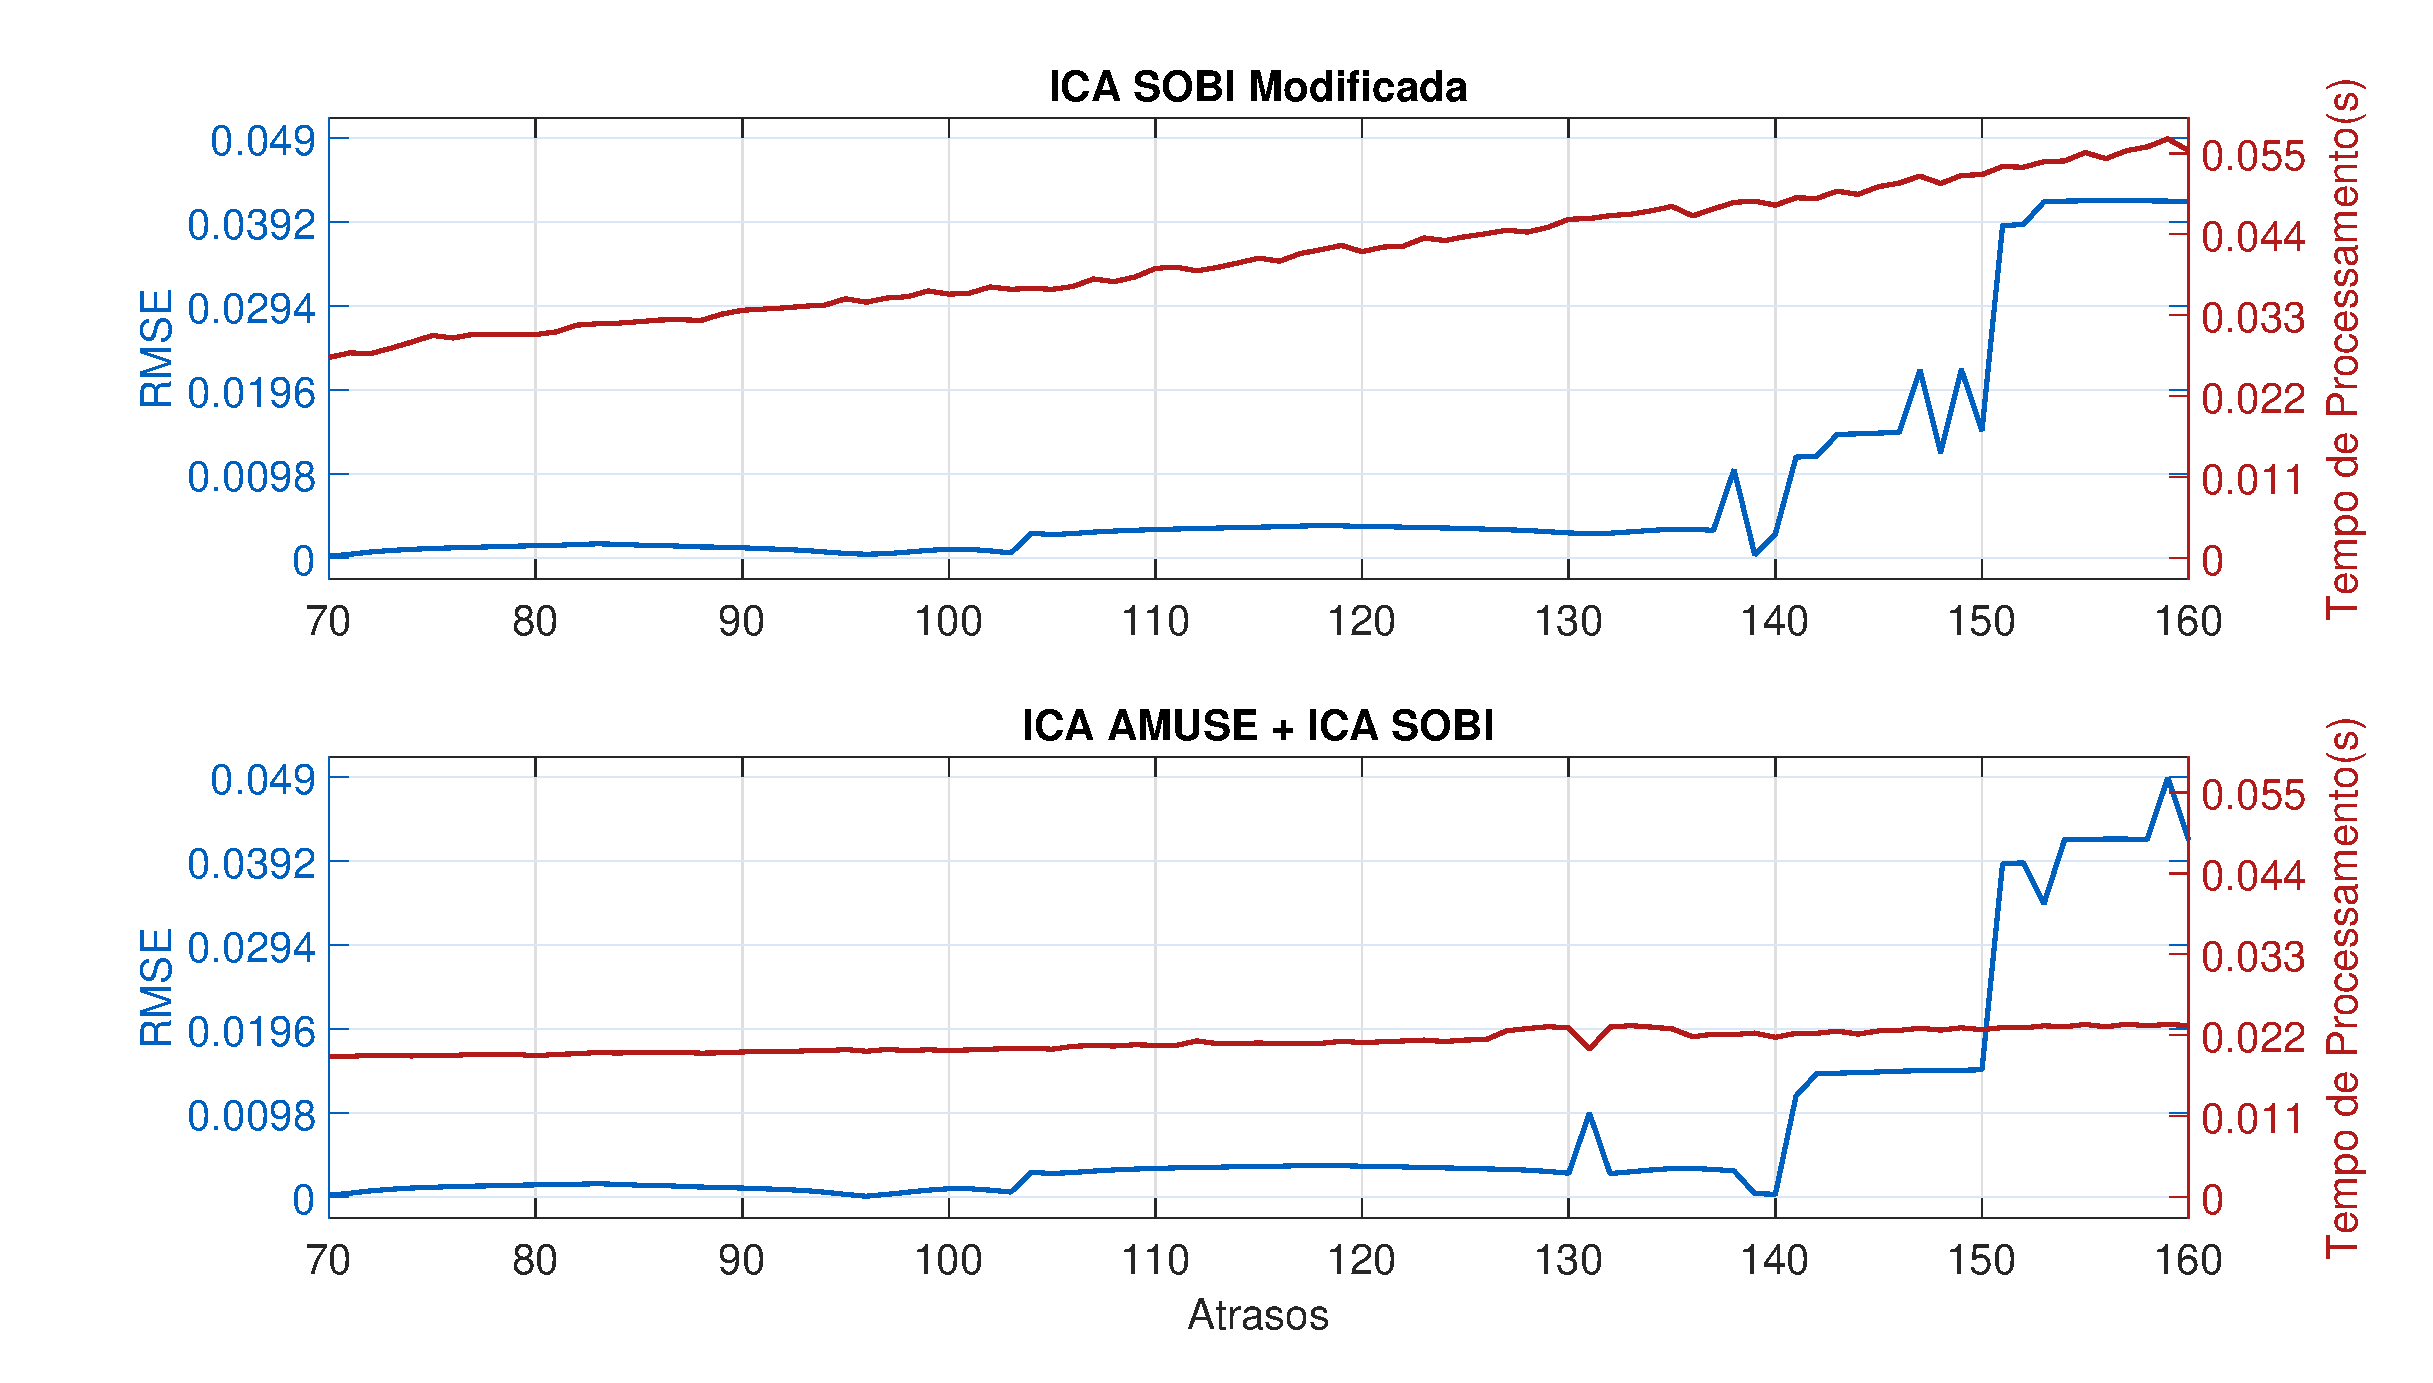
\includegraphics[scale=0.45]{imagens/Sinal1Atrasov2.eps}
    \caption{Resultado da variação do número de atrasos para S1.}
    \label{fig:atrasoS1}
    \end{center}
\end{figure}

A Figura \ref{fig:atrasoS2} mostra diversos picos de $\overline{RMSE}$, sendo que esses se devem a um sorteio de fases mais difícil de se separar, além de que para o sinal $S2$ alguns harmônicos/inter-harmônicos possuem uma amplitude bem inferior à amplitude da fundamental. Apesar desses picos, pode-se perceber um comportamento geral semelhante para ambas as ICAs. Chama a atenção um comportamento em uma forma ondular do $\overline{RMSE}$, com um mínimo em $m=90$ ou próximo dele, e um máximo em $m=120$ e outro em $m=48$, onde se começa o teste. Vale destacar também que, como na Figura \ref{fig:atrasoS1}, o $\overline{TP}$ para a combinação de ICAs é relativamente menor que o $\overline{TP}$ para a ICA SOBI modificada. Por fim, para todos os valores de $m$ testados, o tempo de processamento para ambas as ICAs se manteve inferior ao tempo de obtenção do sinal ($TO=0.20$s).

\begin{figure}[!htb]
    \begin{center}
    \advance\leftskip -1.5cm
    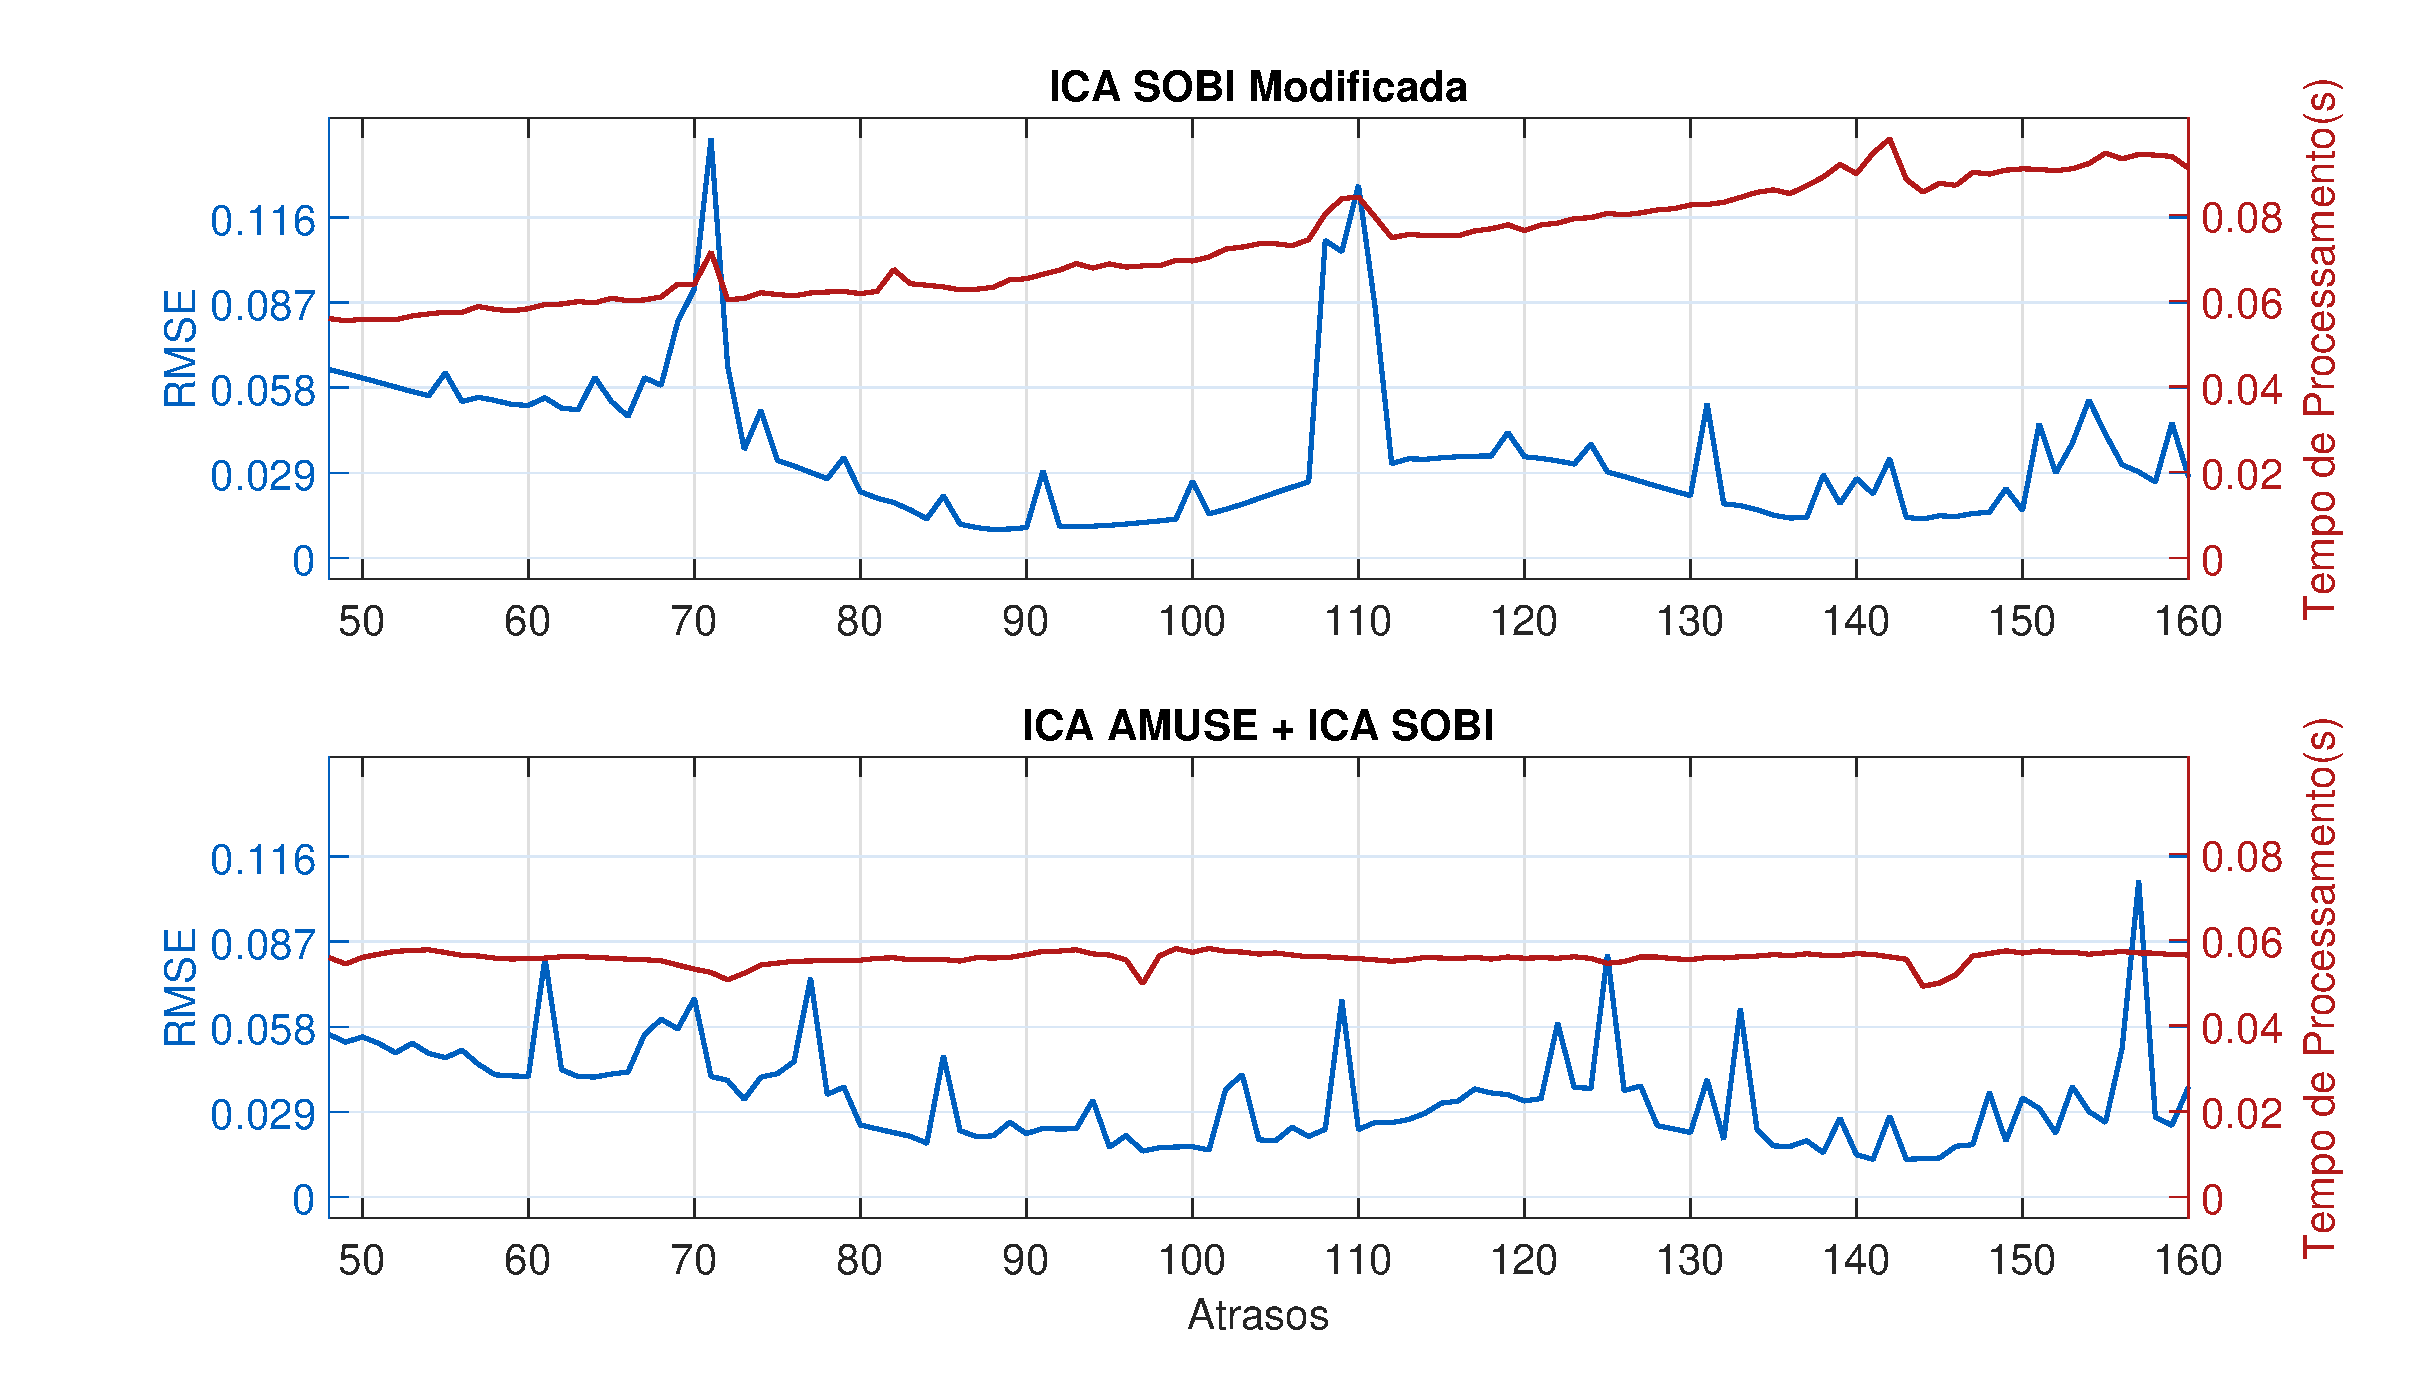
\includegraphics[scale=0.45]{imagens/Sinal2Atrasov2.eps}
    \caption{Resultado da variação do número de atrasos para S2.}
    \label{fig:atrasoS2}
    \end{center}
\end{figure}

Observa-se na Figura \ref{fig:atrasoS3} que para o teste com o sinal $S3$, a combinação de ICAs não foi capaz de estimar um bom resultado para um baixo número de atrasos. Pode-se aqui também perceber que o $\overline{RMSE}$ possui um comportamento oscilatório em relação ao aumento do número de atrasos, tendo os melhores resultados para $m=100$, $m=200$ e $m=300$. Assim como para os testes em $S1$ e $S2$, o $\overline{TP}$ para a combinação de ICAs é menor que o $\overline{TP}$ para a ICA SOBI modificada, percebendo-se para este último um comportamento exponencial. Também aqui, para todos os valores de $m$ testados, $\overline{TP}$ foi menor que $TO=1$s para ambas as ICAs.

\begin{figure}[!htb]
    \begin{center}
    \advance\leftskip -1.5cm
    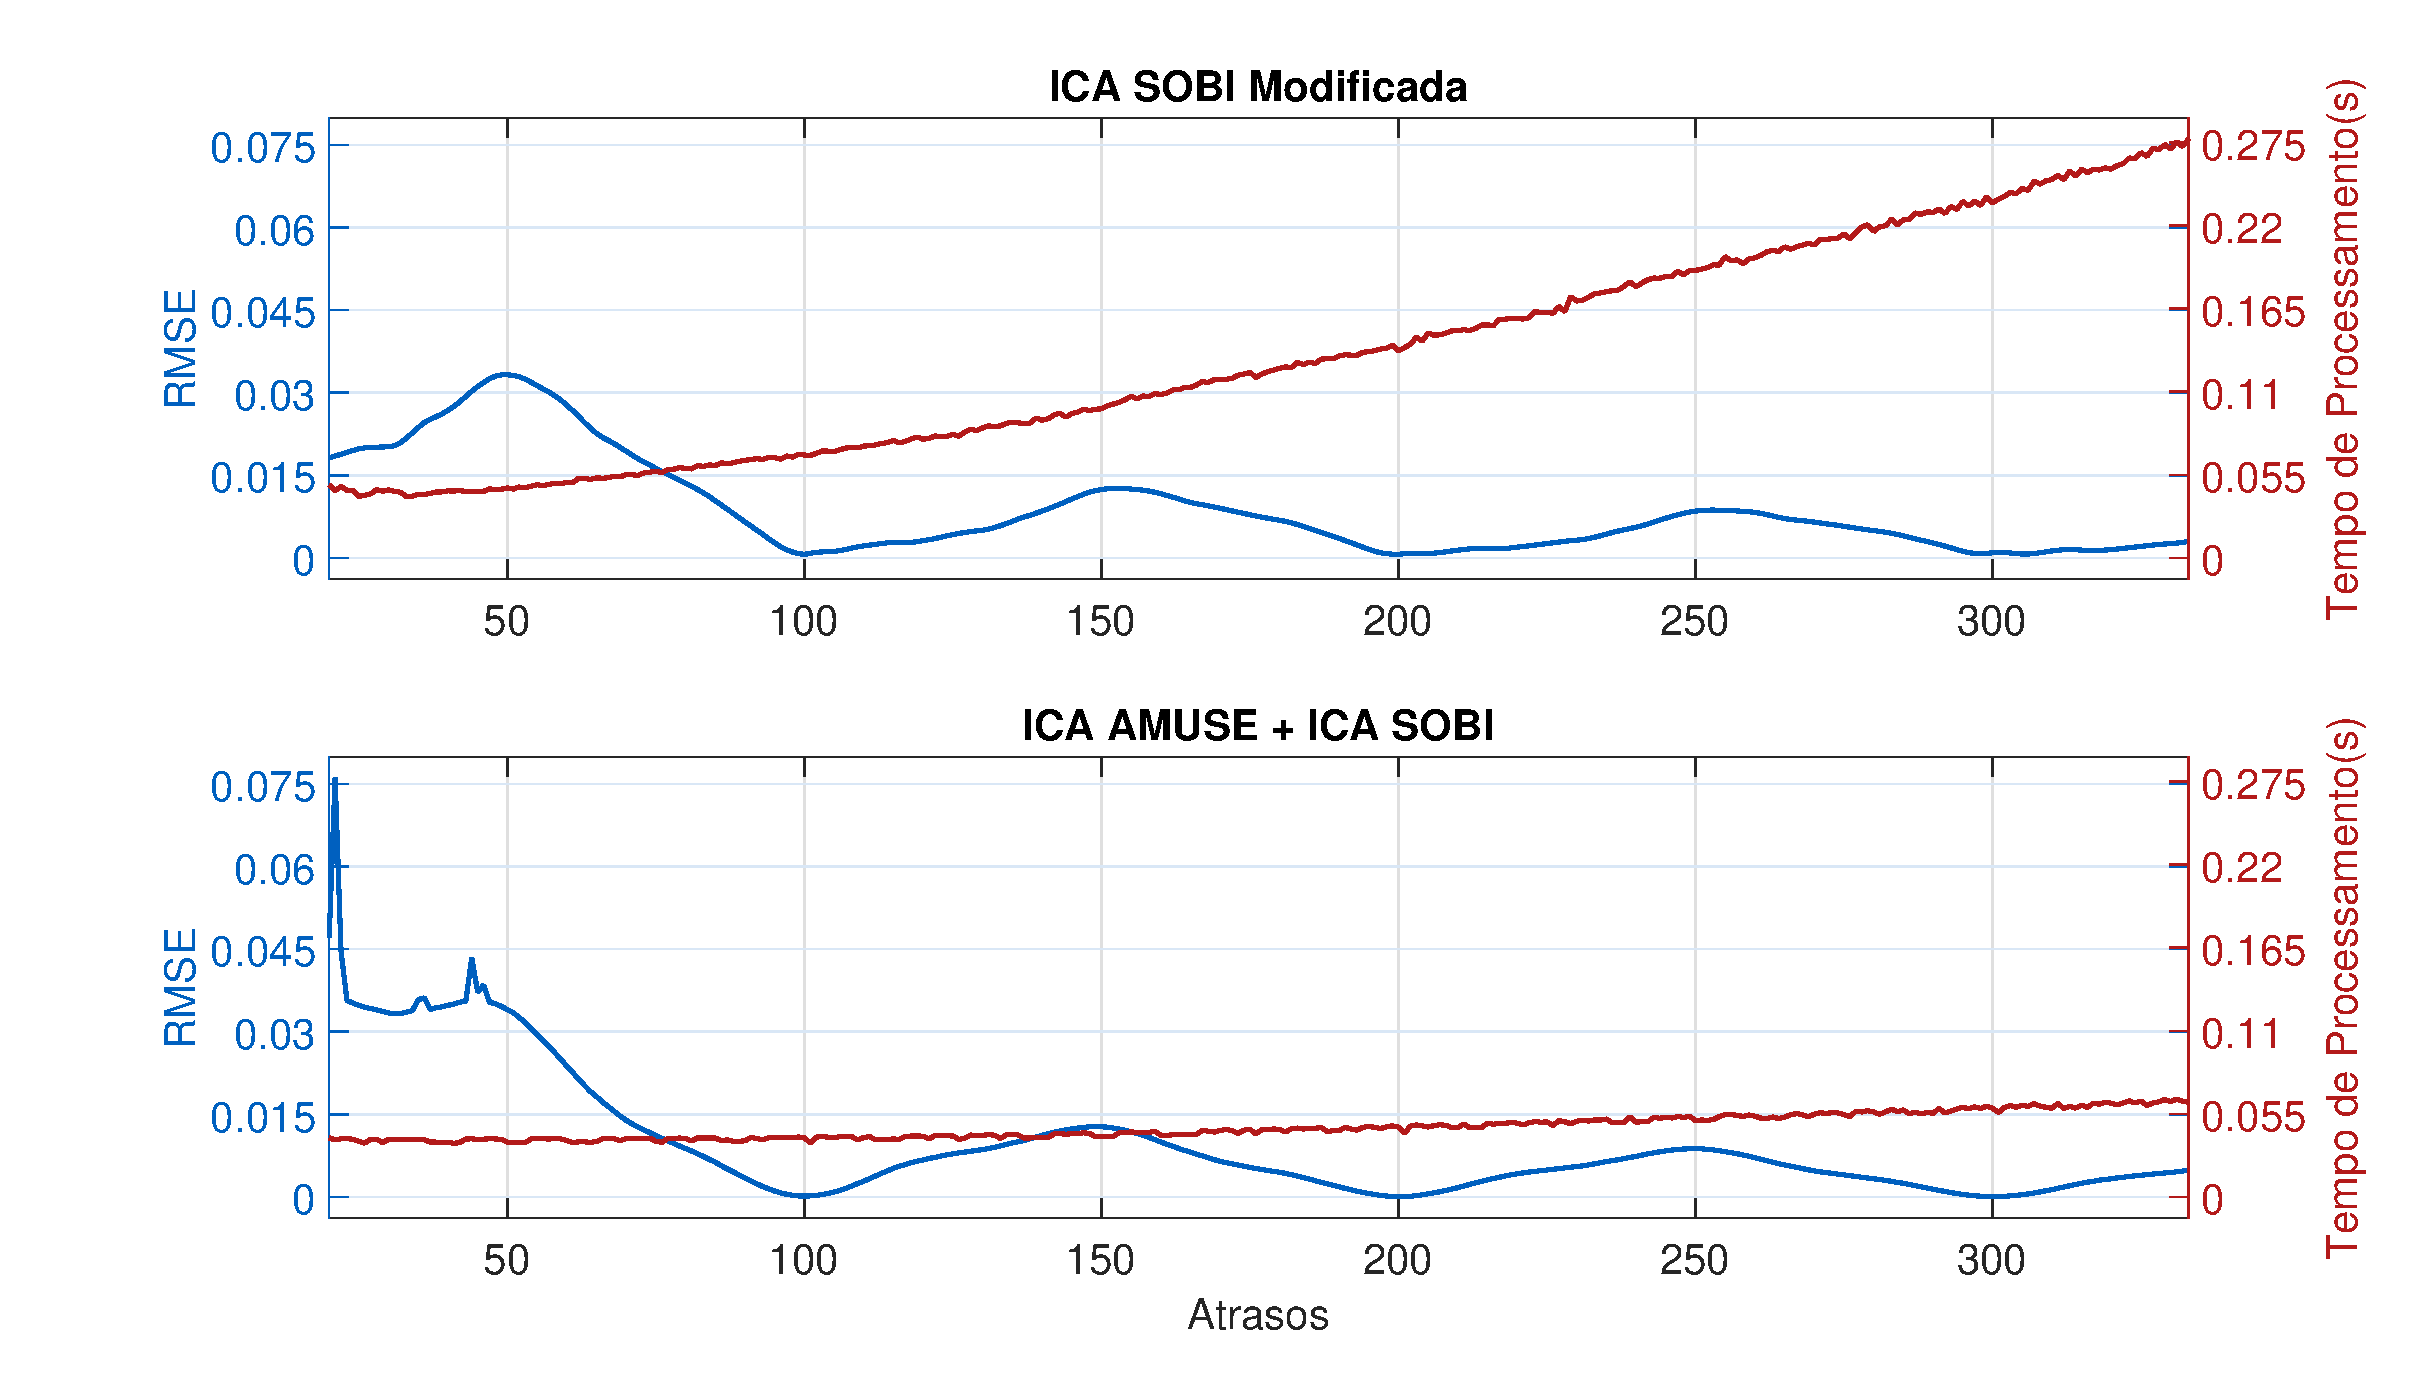
\includegraphics[scale=0.45]{imagens/Sinal3Atrasov2.eps}
    \caption{Resultado da variação do número de atrasos para S3.}
    \label{fig:atrasoS3}    
    \end{center}
\end{figure}

Na Figura \ref{fig:atrasoS4}, correspondente ao teste realizado para o sinal $S4$, tem-se um comportamento anormal e não visto nos testes anteriores. Percebe-se que ocorrem picos no $\overline{TP}$ da ICA SOBI Modificada para alguns valores de $m$. Foi realizada uma investigação minuciosa e constatado que esses picos de $\overline{TP}$ têm origem em três blocos de processamento do método proposto: agrupamento, recuperação de amplitude e na própria ICA. Pode-se também observar que neste teste o comportamento do $\overline{RMSE}$ para ambas as ICAs se apresenta de forma muito diferente em função de $m$, não tendo um padrão peculiar como ocorreu para os testes anteriores. Porém, percebe-se que de maneira geral a Combinação de ICAs apresentou menores valores de $\overline{RMSE}$ para diferentes valores de $m$. Finalmente, para este teste, o $TP$ para a ICA SOBI Modificada apresentou valores maiores do que $TO=0.20$s para valores mais elevados de $m$. Já para a Combinação de ICAs, $\overline{TP}$ se manteve sempre menor do que $TO$.

\begin{figure}[!htb]
    \begin{center}
    \advance\leftskip -1.5cm
    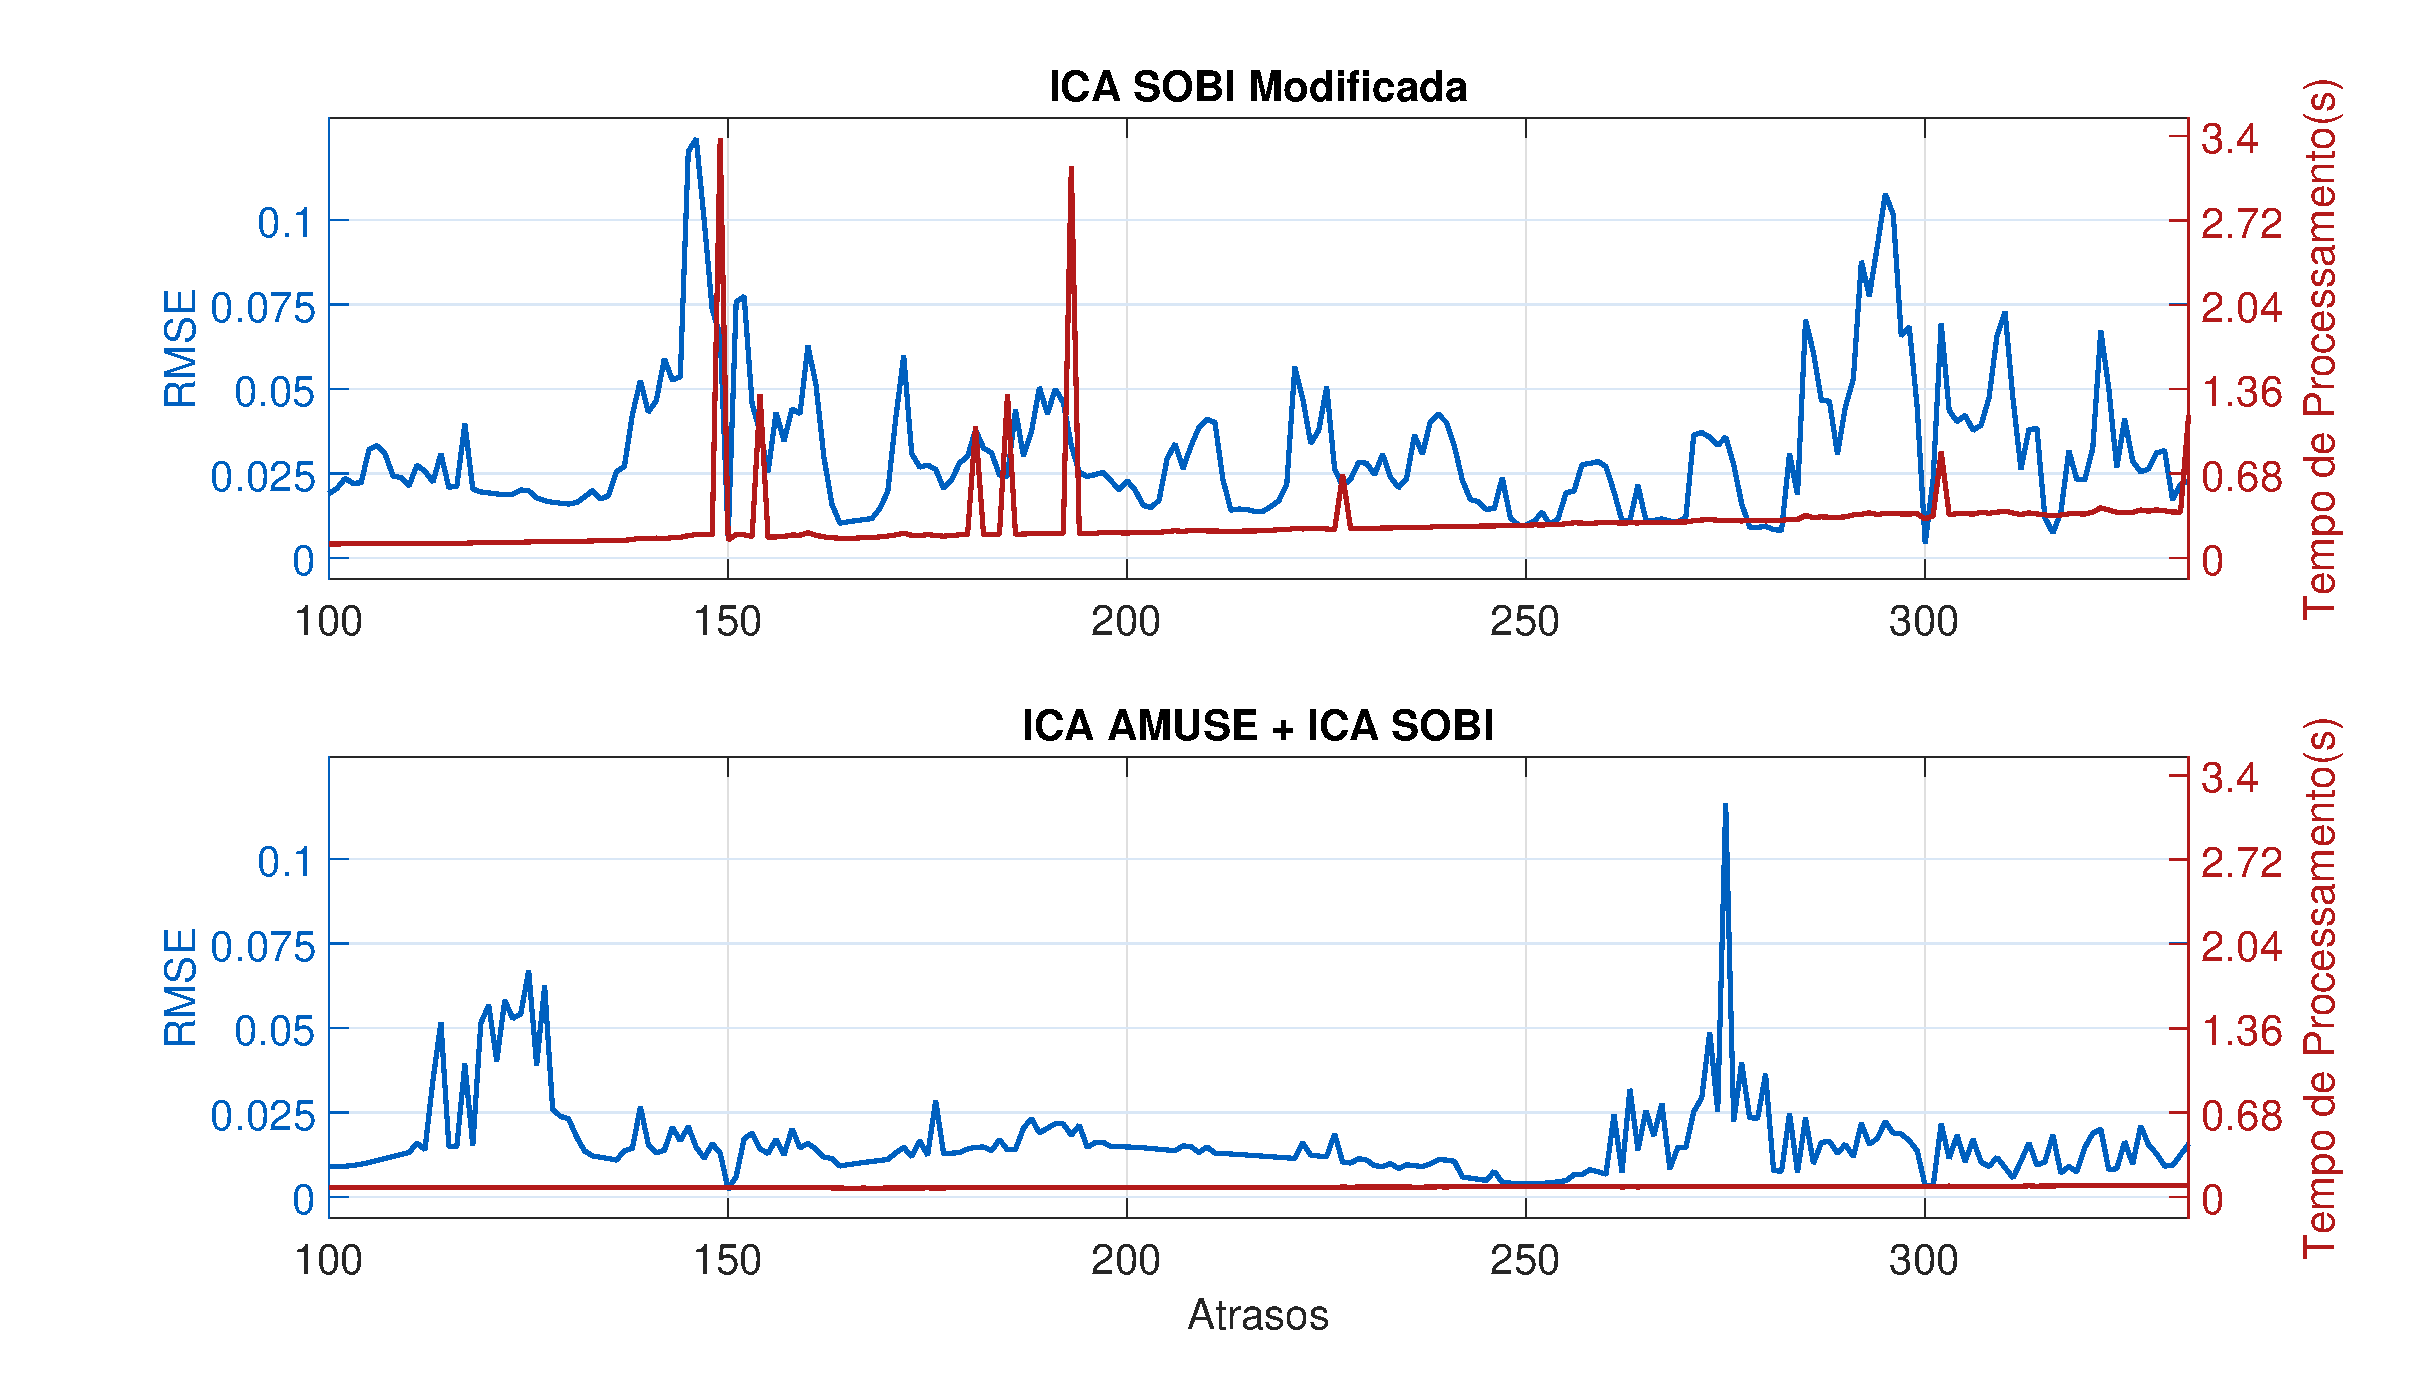
\includegraphics[scale=0.45]{imagens/Sinal4Atrasov2.eps}
    \caption{Resultado da variação do número de atrasos para S4.}
    \label{fig:atrasoS4}
    \end{center}
\end{figure}

A Figura \ref{fig:atrasoS5}, correspondente ao teste do sinal $S5$, mostra um comportamento do $\overline{RMSE}$ semelhante ao ocorrido na Figura \ref{fig:atrasoS3}. Vale destacar que ocorre um mínimo global quando o número de atrasos é igual a 80, ou seja, para $m$ igual ao número de amostras correspondentes a 2 ciclos da fundamental. Assim como em todos os testes anteriores, o $\overline{TP}$ da Combinação de ICAs é menor que o $\overline{TP}$ da ICA SOBI Modificada. Para ambas as ICAs, $\overline{TP}$ foi menor que $TO=0.20$s, para todos os valores de $m$ testados.

\begin{figure}[!htb]
    \begin{center}
    \advance\leftskip -1.5cm
    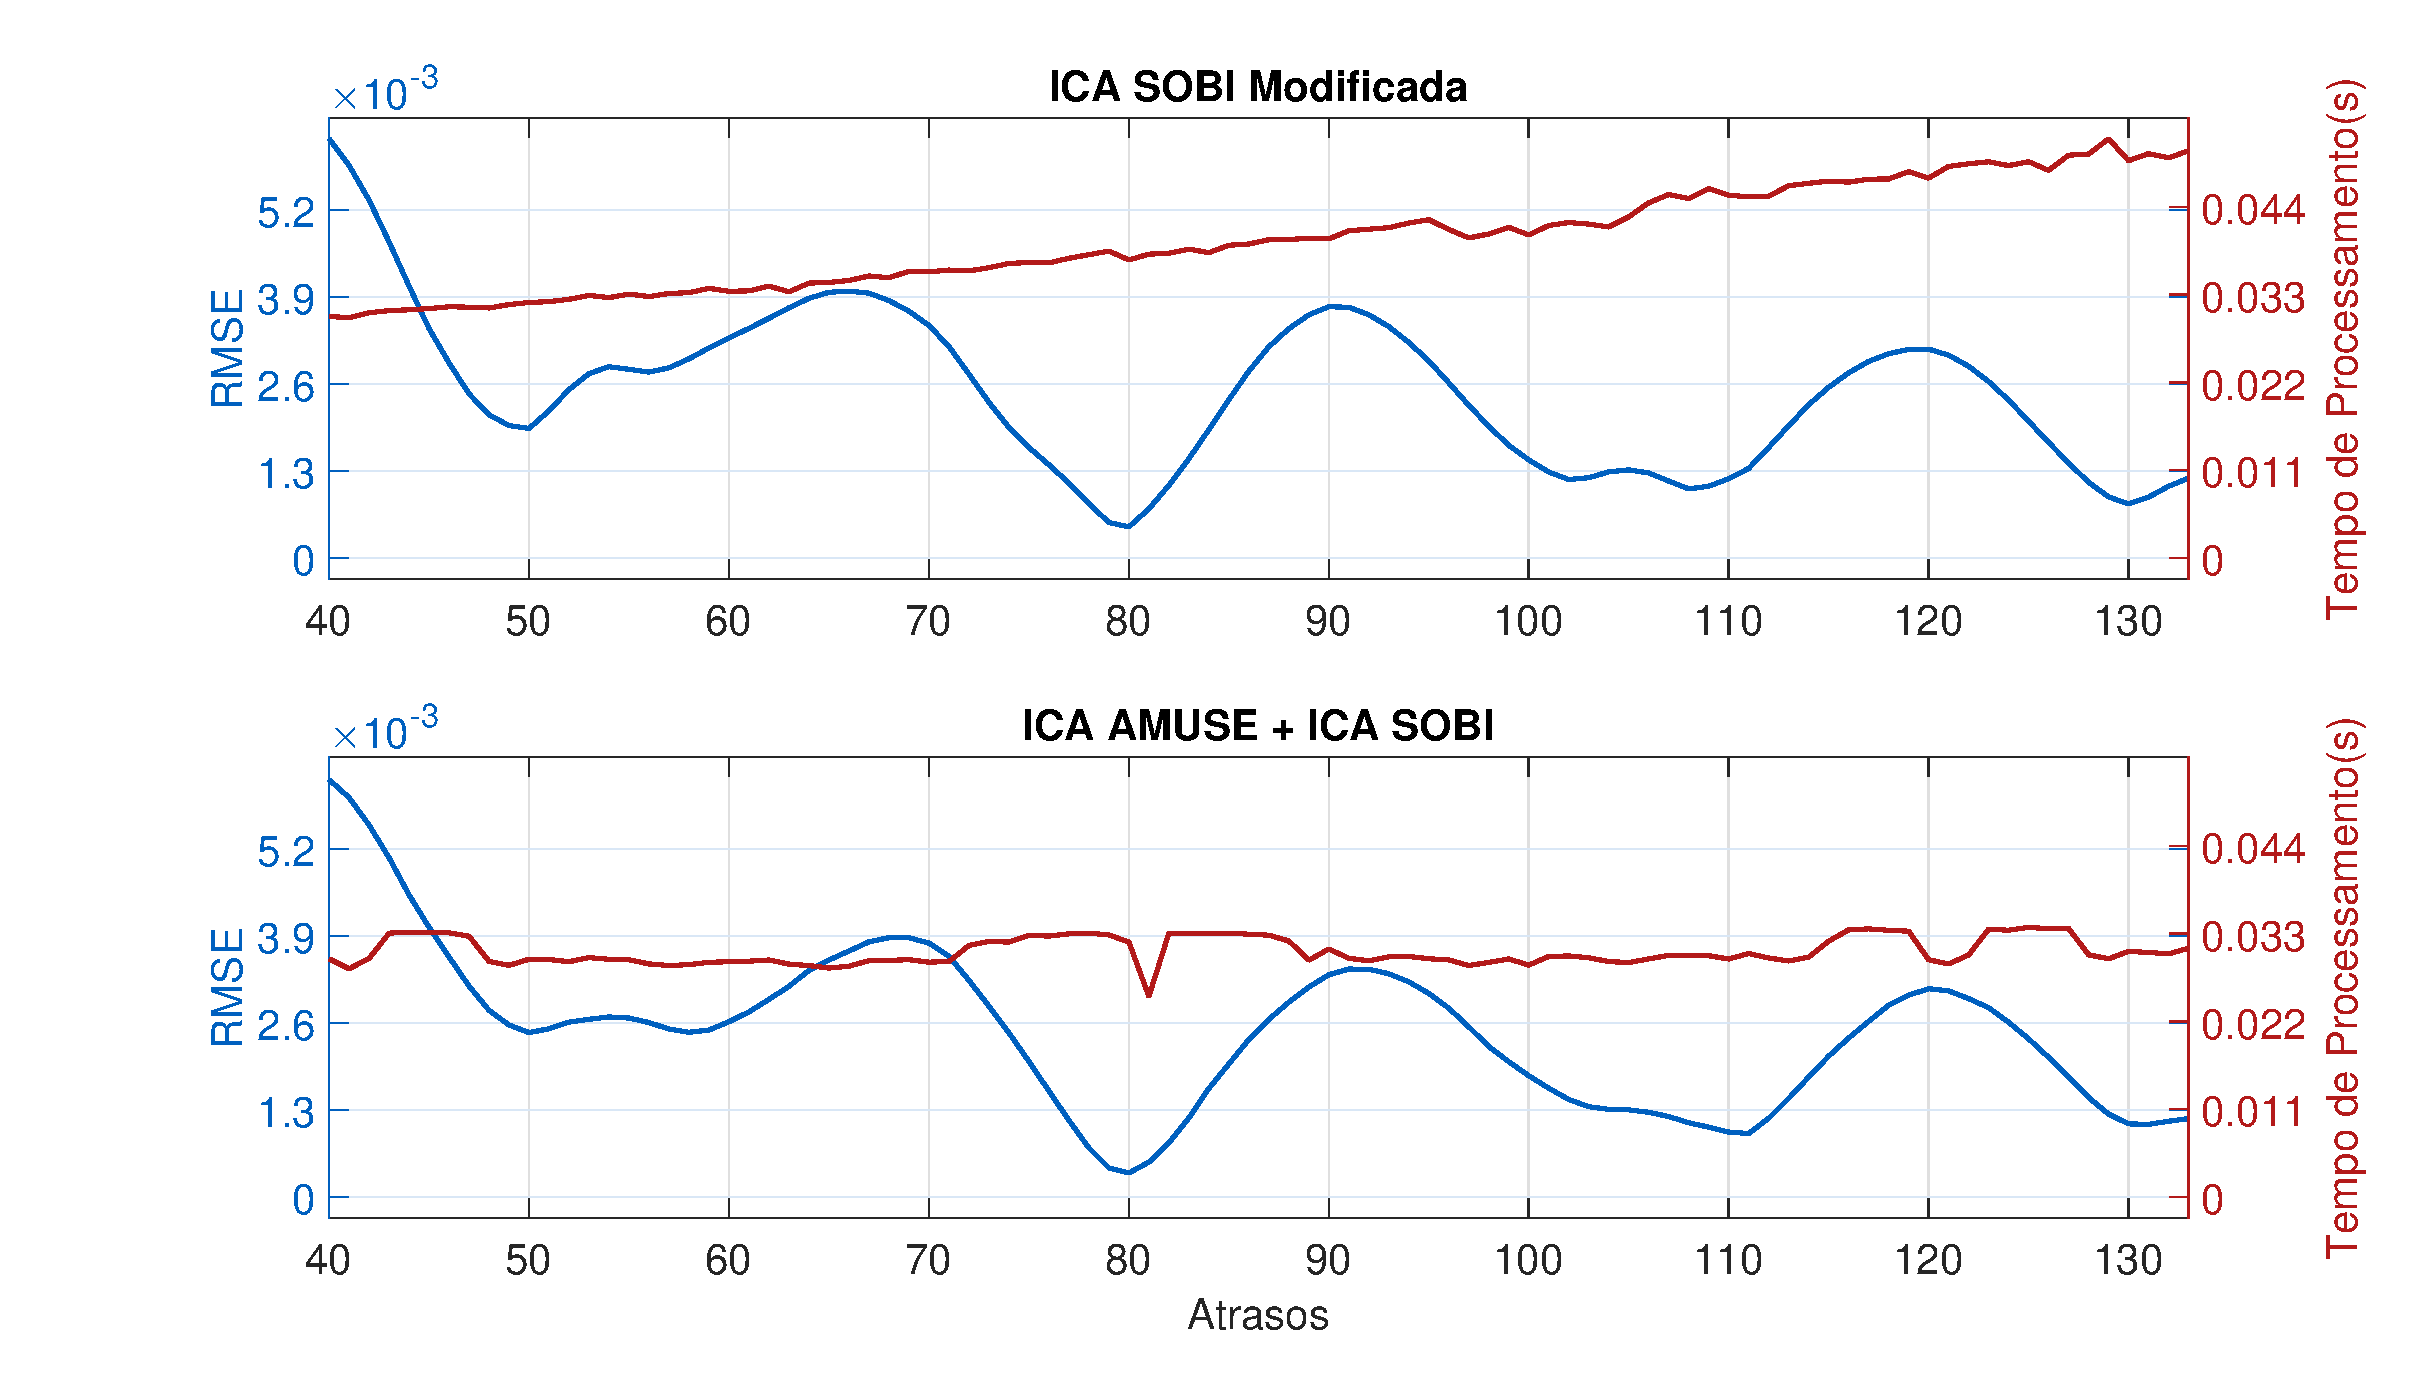
\includegraphics[scale=0.45]{imagens/Sinal5Atrasov2.eps}
    \caption{Resultado da variação do número de atrasos para S5.}
    \label{fig:atrasoS5}
    \end{center}
\end{figure}

Analisando-se as Figuras \ref{fig:atrasoS1} a \ref{fig:atrasoS5}, pode-se perceber que para qualquer um dos sinais testados, dado que a SNRdb foi elevada (SRNdb=100~dB), um número de atrasos pertinente a ser escolhido é $N_s/5$. Nas Figuras \ref{fig:atrasoS1} e \ref{fig:atrasoS2}, este número é igual a 96, para o qual pode-se dizer que ocorrem um baixo $\overline{RMSE}$ e um baixo $\overline{TP}$. Já nas Figuras \ref{fig:atrasoS3} e \ref{fig:atrasoS4}, esse número é igual a 200, que na Figura \ref{fig:atrasoS3} corresponde nitidamente a um mínimo de $\overline{RMSE}$ e na Figura \ref{fig:atrasoS4} é uma boa escolha. Por último, na Figura \ref{fig:atrasoS5}, o número ideal é 80, que é exatamente o valor de $m$ correspondente ao mínimo global de $\overline{RMSE}$. Também pode-se perceber que em todas as Figuras, o $\overline{TP}$ é menor que o $TO$, exceto para os valores de $m$ para os quais ocorreram picos de tempo de processamento.  

\section{Sensibilidade ao Ruído}
\label{ch:testeRU}

Como constatado na sessão anterior, um número de atrasos ideal seria $m=N_s$/5 amostras. Porém, este número só é considerado ideal para um alto valor da relação sinal ruído (SNRdb). Então, com o intuito de garantir um melhor resultado para um sinal ruidoso, foram realizados testes com um número de atrasos ligeiramente maior, com o valor $m=round(N_s/4.8)$, onde $round(.)$ aproxima o valor de seu argumento para o inteiro mais próximo.

Os resultados para os testes de sensibilidade ao ruído aplicado aos sinais $S1$ a $S5$ podem ser vistos nas Figuras \ref{fig:ruidos1} a \ref{fig:ruidos5}. Em cada figura, o eixo de abcissa corresponde à SNRdb, a curva em azul corresponde ao $\overline{RMSE}$ e a curva em vermelho corresponde ao $\overline{TP}$ do método proposto, considerando-se apenas as ICAs Sobi Modificada e ICA AMUSE combinada com a ICA SOBI Modificada.

\begin{figure}[!htb]
    \begin{center}
    \advance\leftskip -1.5cm
    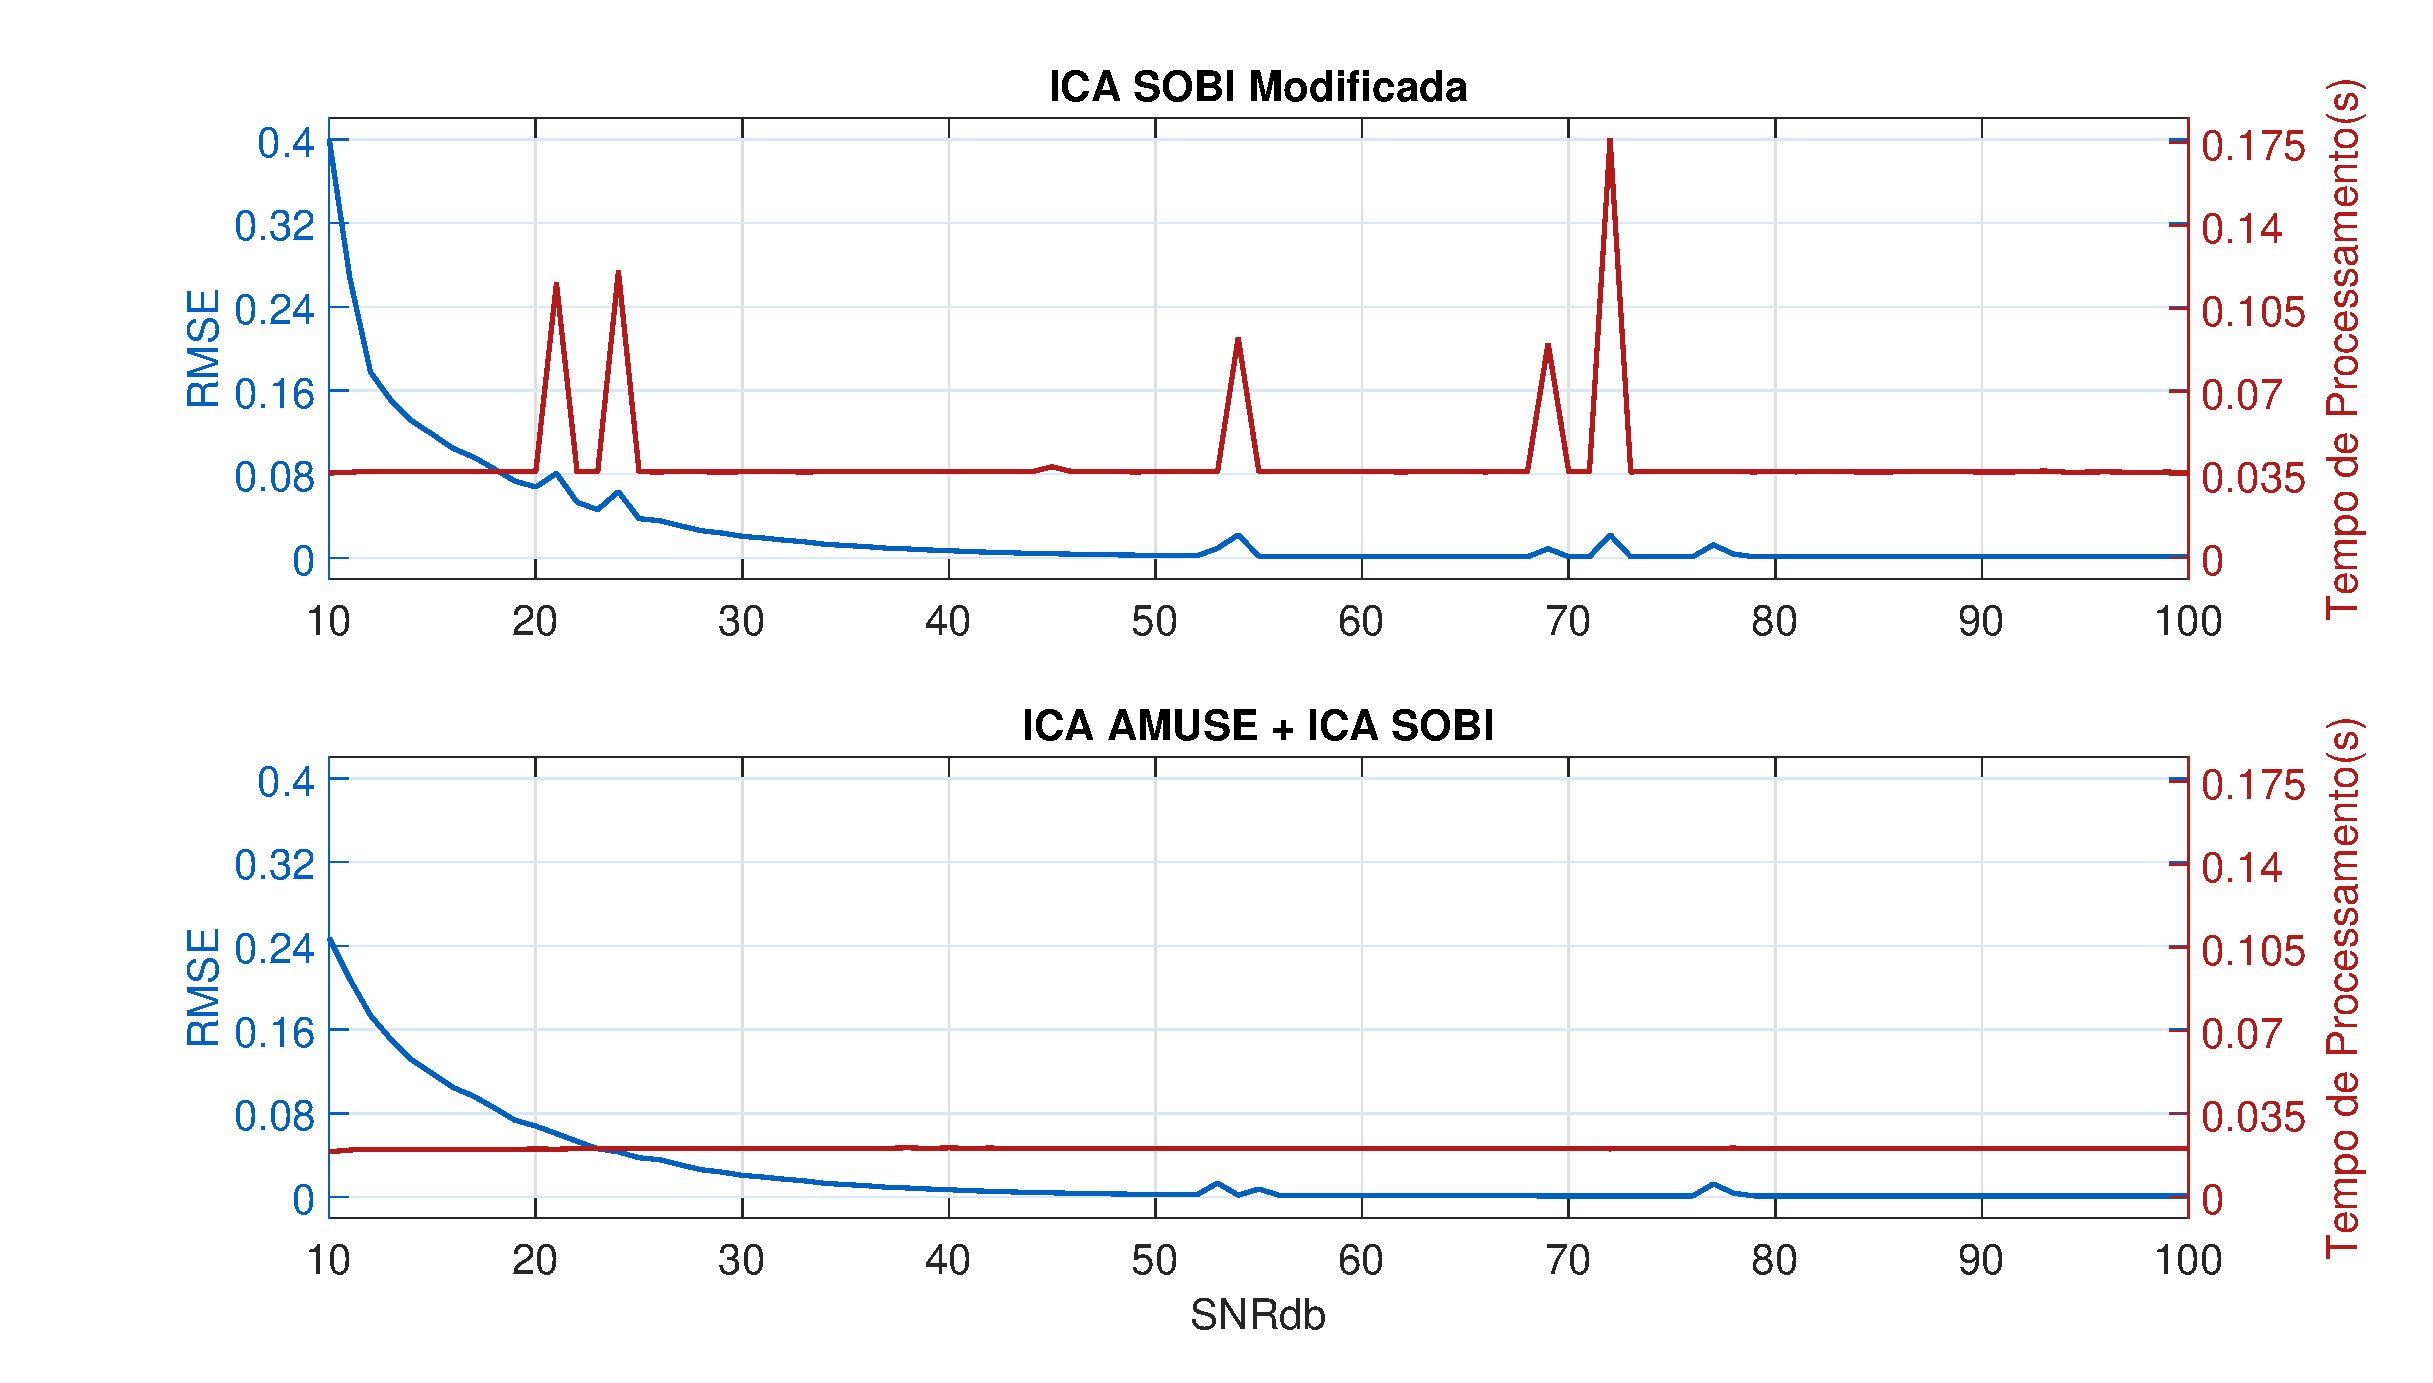
\includegraphics[scale=0.45]{imagens/Sinal1Ruidov2.eps}
    \caption{Resultado da variação do SNRdb para o S1}
    \label{fig:ruidos1}    
    \end{center}
\end{figure}

\begin{figure}[!htb]
    \begin{center}
    \advance\leftskip -1.5cm
    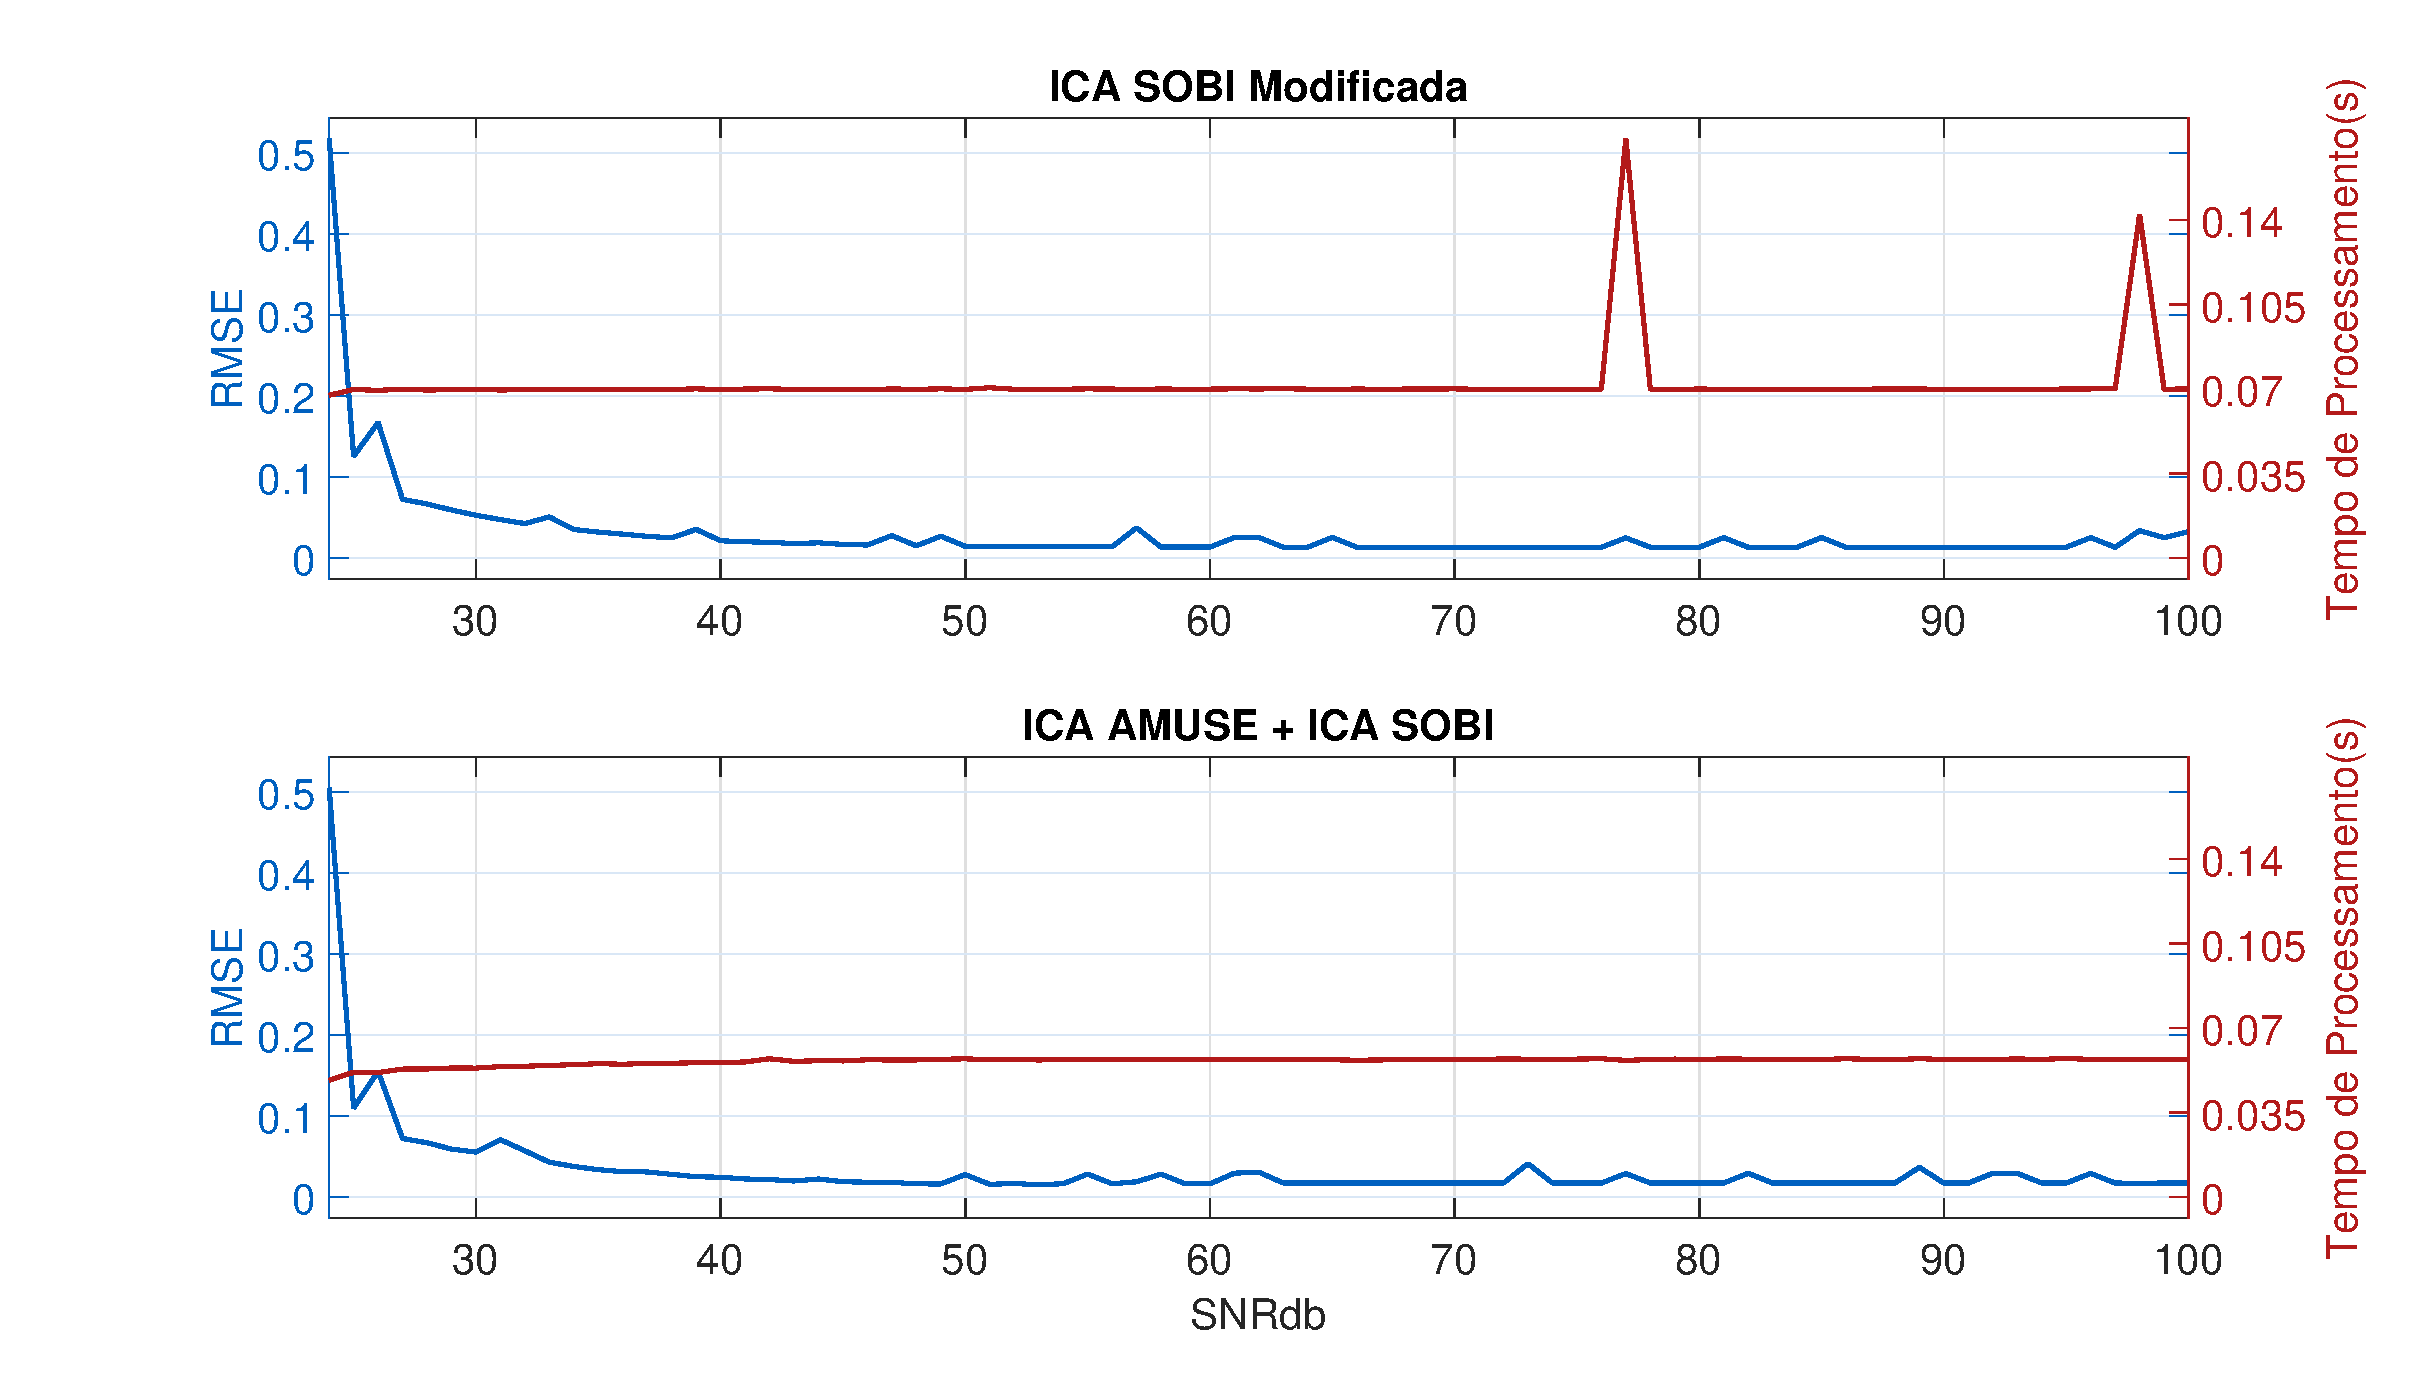
\includegraphics[scale=0.45]{imagens/Sinal2Ruidov2.eps}
    \caption{Resultado da variação do SNRdb para o S2}
    \label{fig:ruidos2}    
    \end{center}
\end{figure}

\begin{figure}[!htb]
    \begin{center}
    \advance\leftskip -1.5cm
    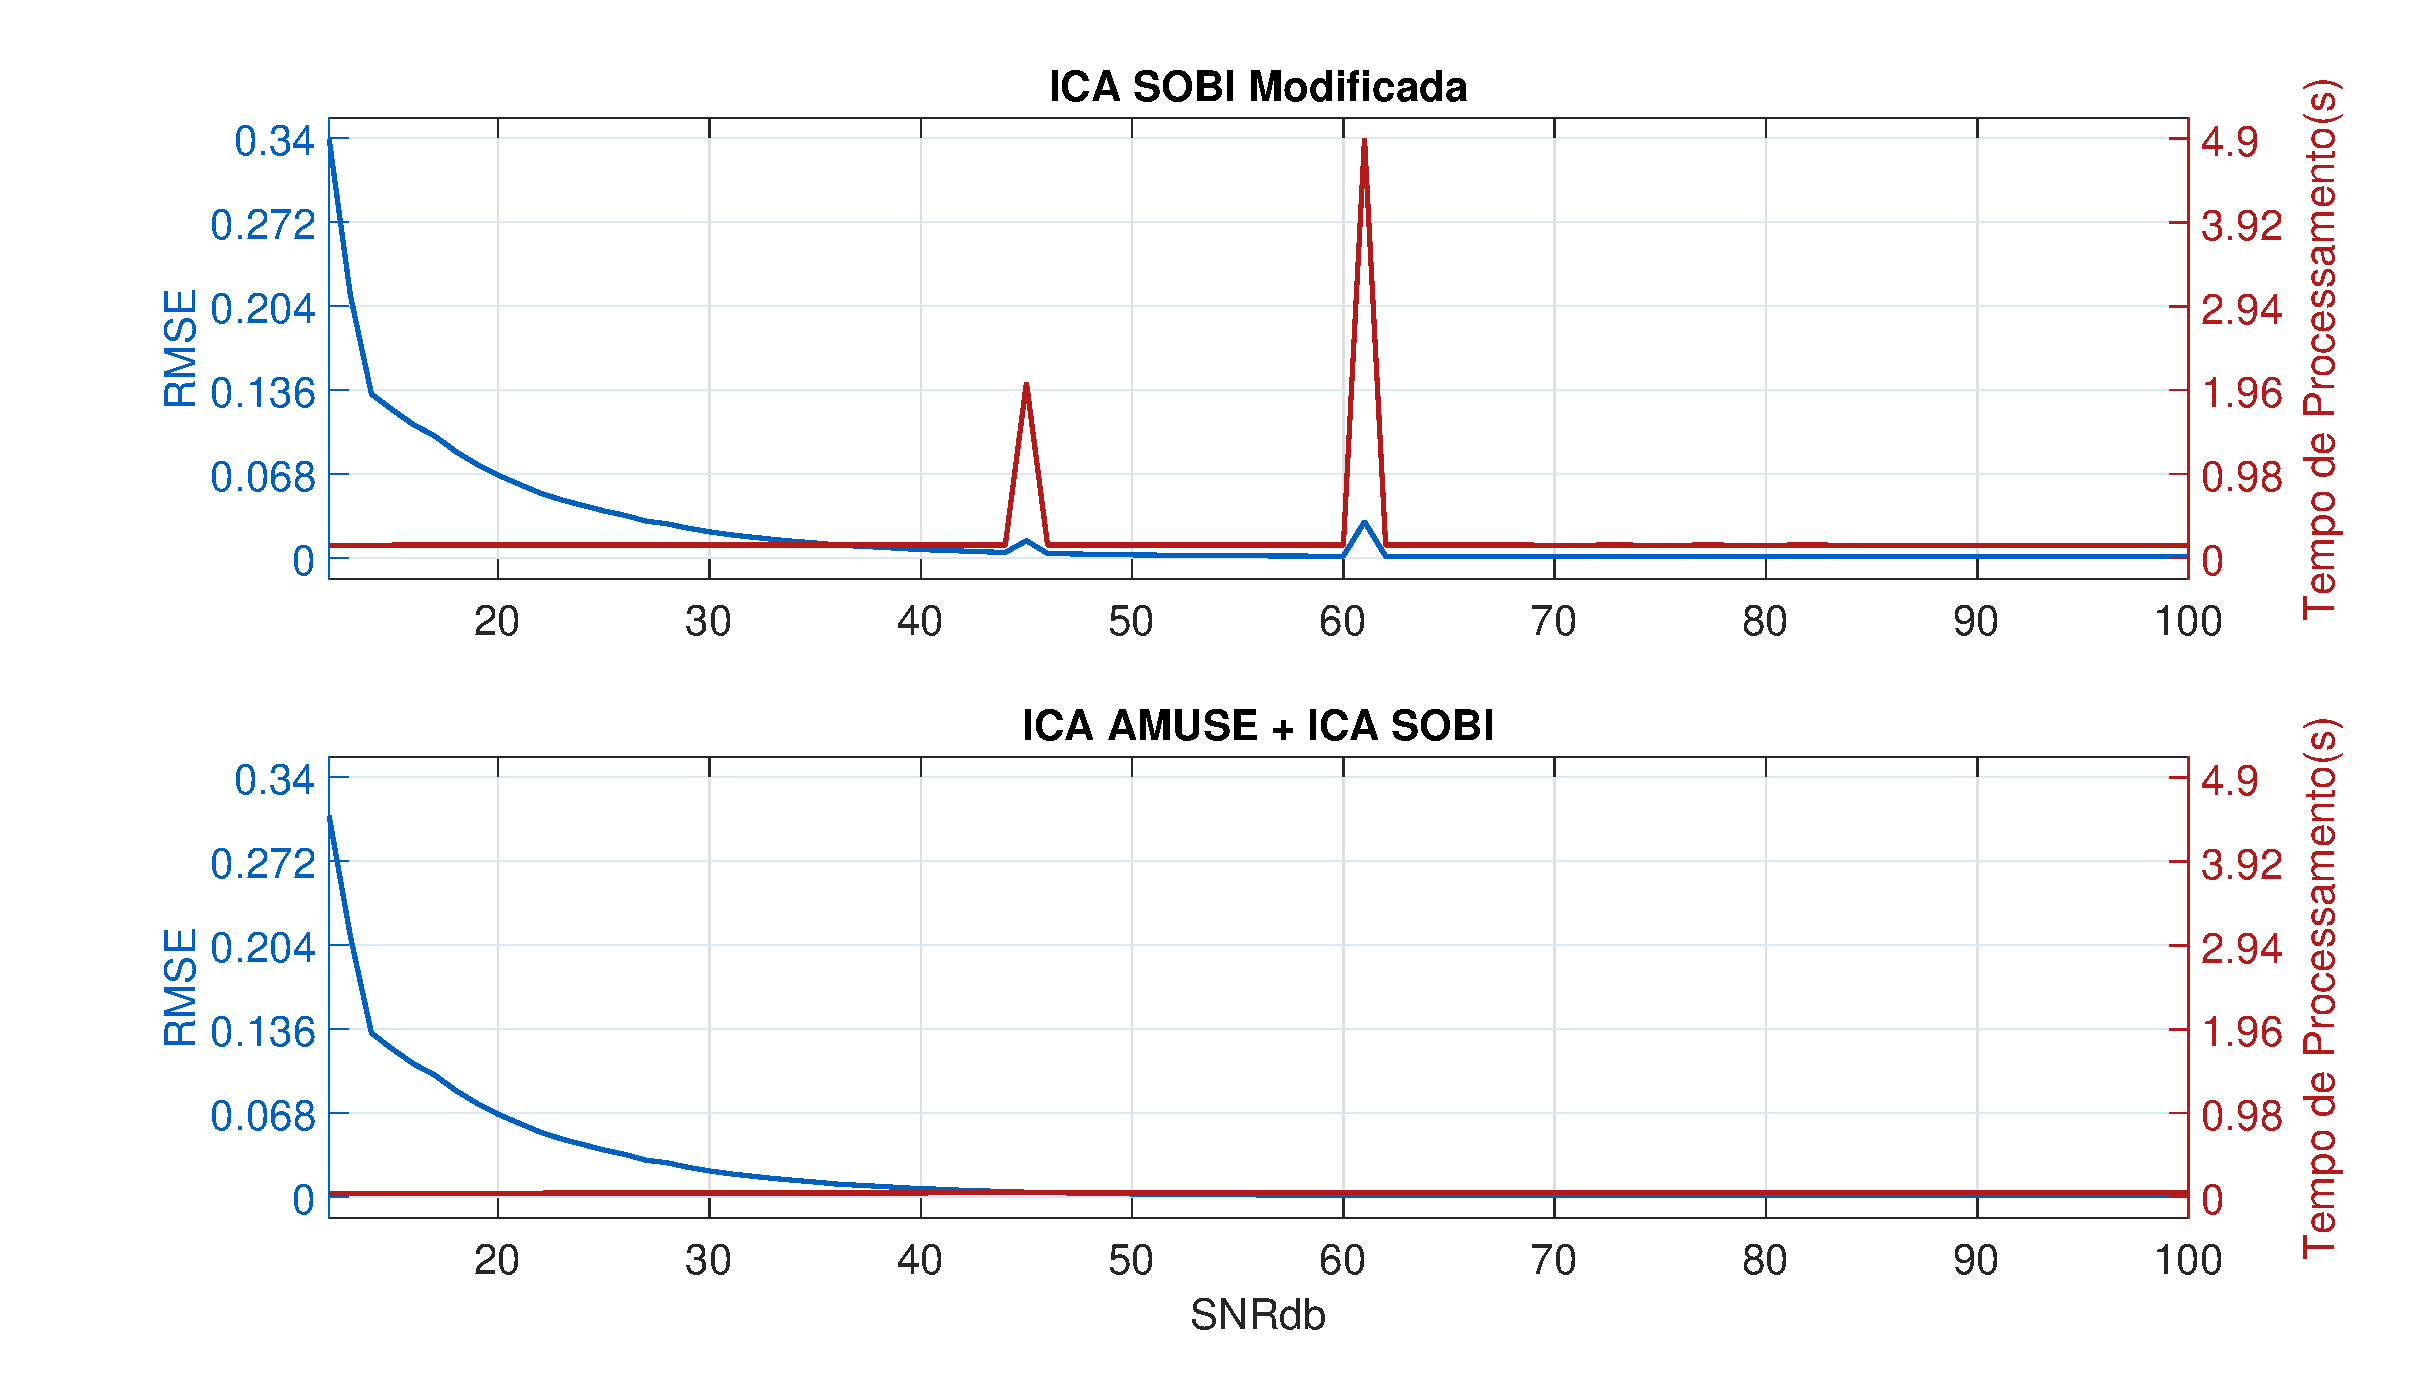
\includegraphics[scale=0.45]{imagens/Sinal3Ruidov2.eps}
    \caption{Resultado da variação do SNRdb para o S3}
    \label{fig:ruidos3}    
    \end{center}
\end{figure}

\begin{figure}[!htb]
    \begin{center}
    \advance\leftskip -1.5cm
    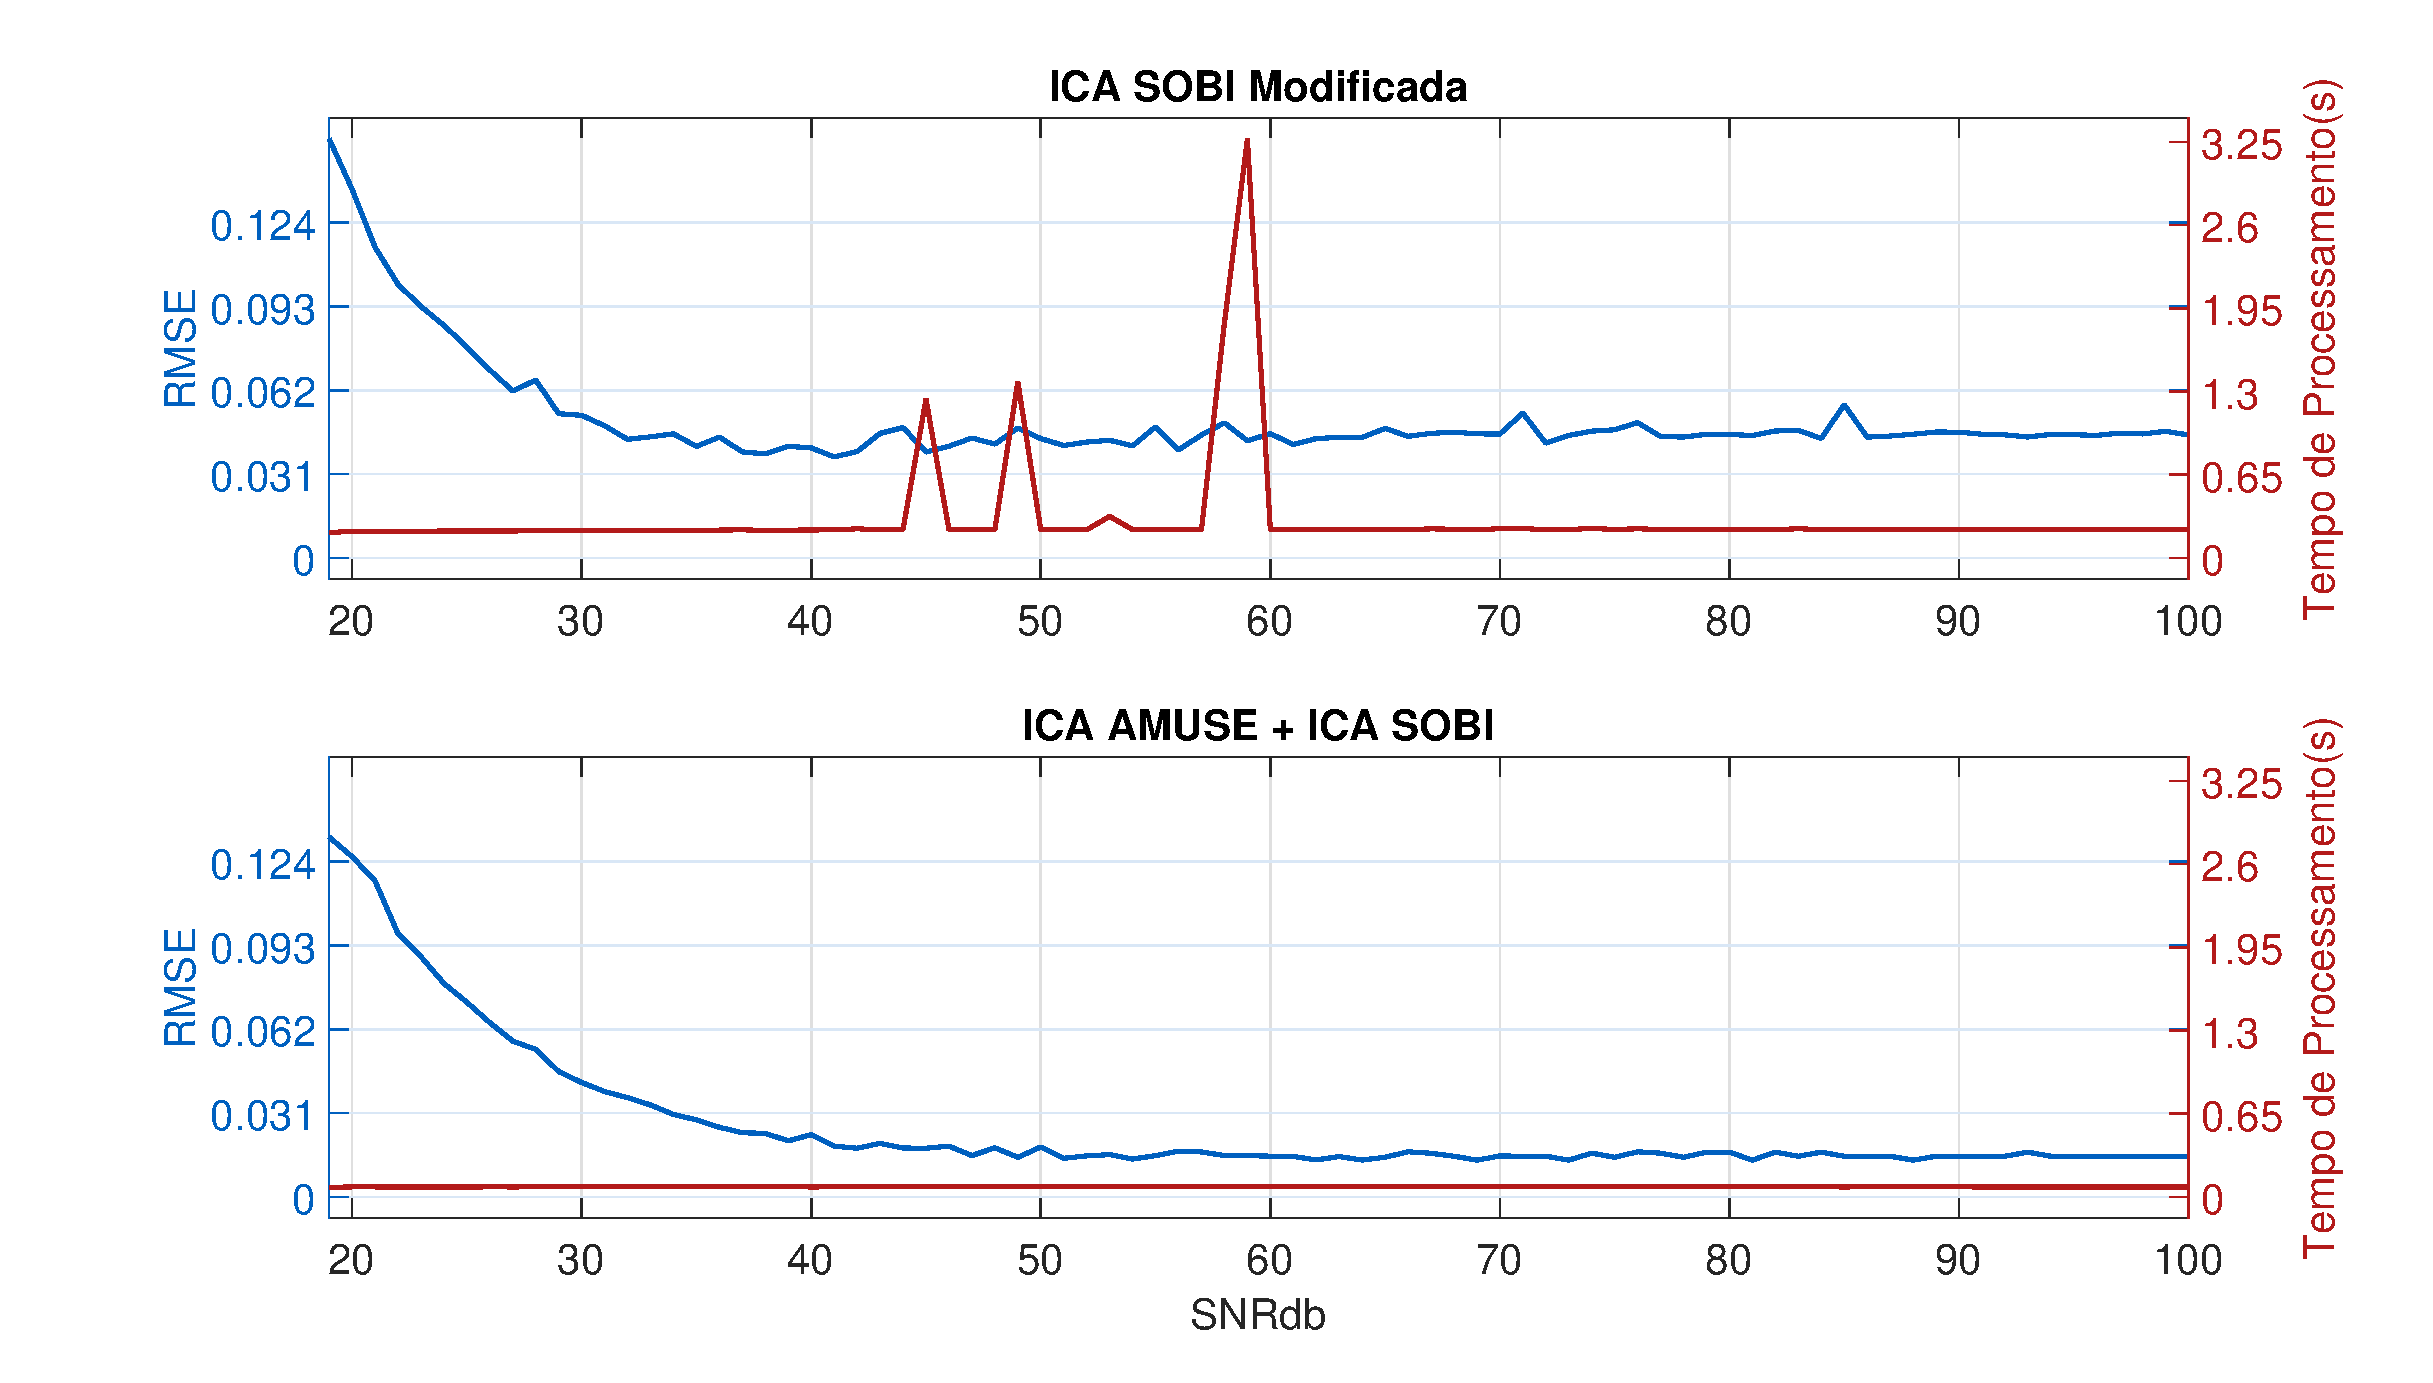
\includegraphics[scale=0.45]{imagens/Sinal4Ruidov2.eps}
    \caption{Resultado da variação do SNRdb para o S4}
    \label{fig:ruidos4}    
    \end{center}
\end{figure}

\begin{figure}[!htb]
    \begin{center}
    \advance\leftskip -1.5cm
    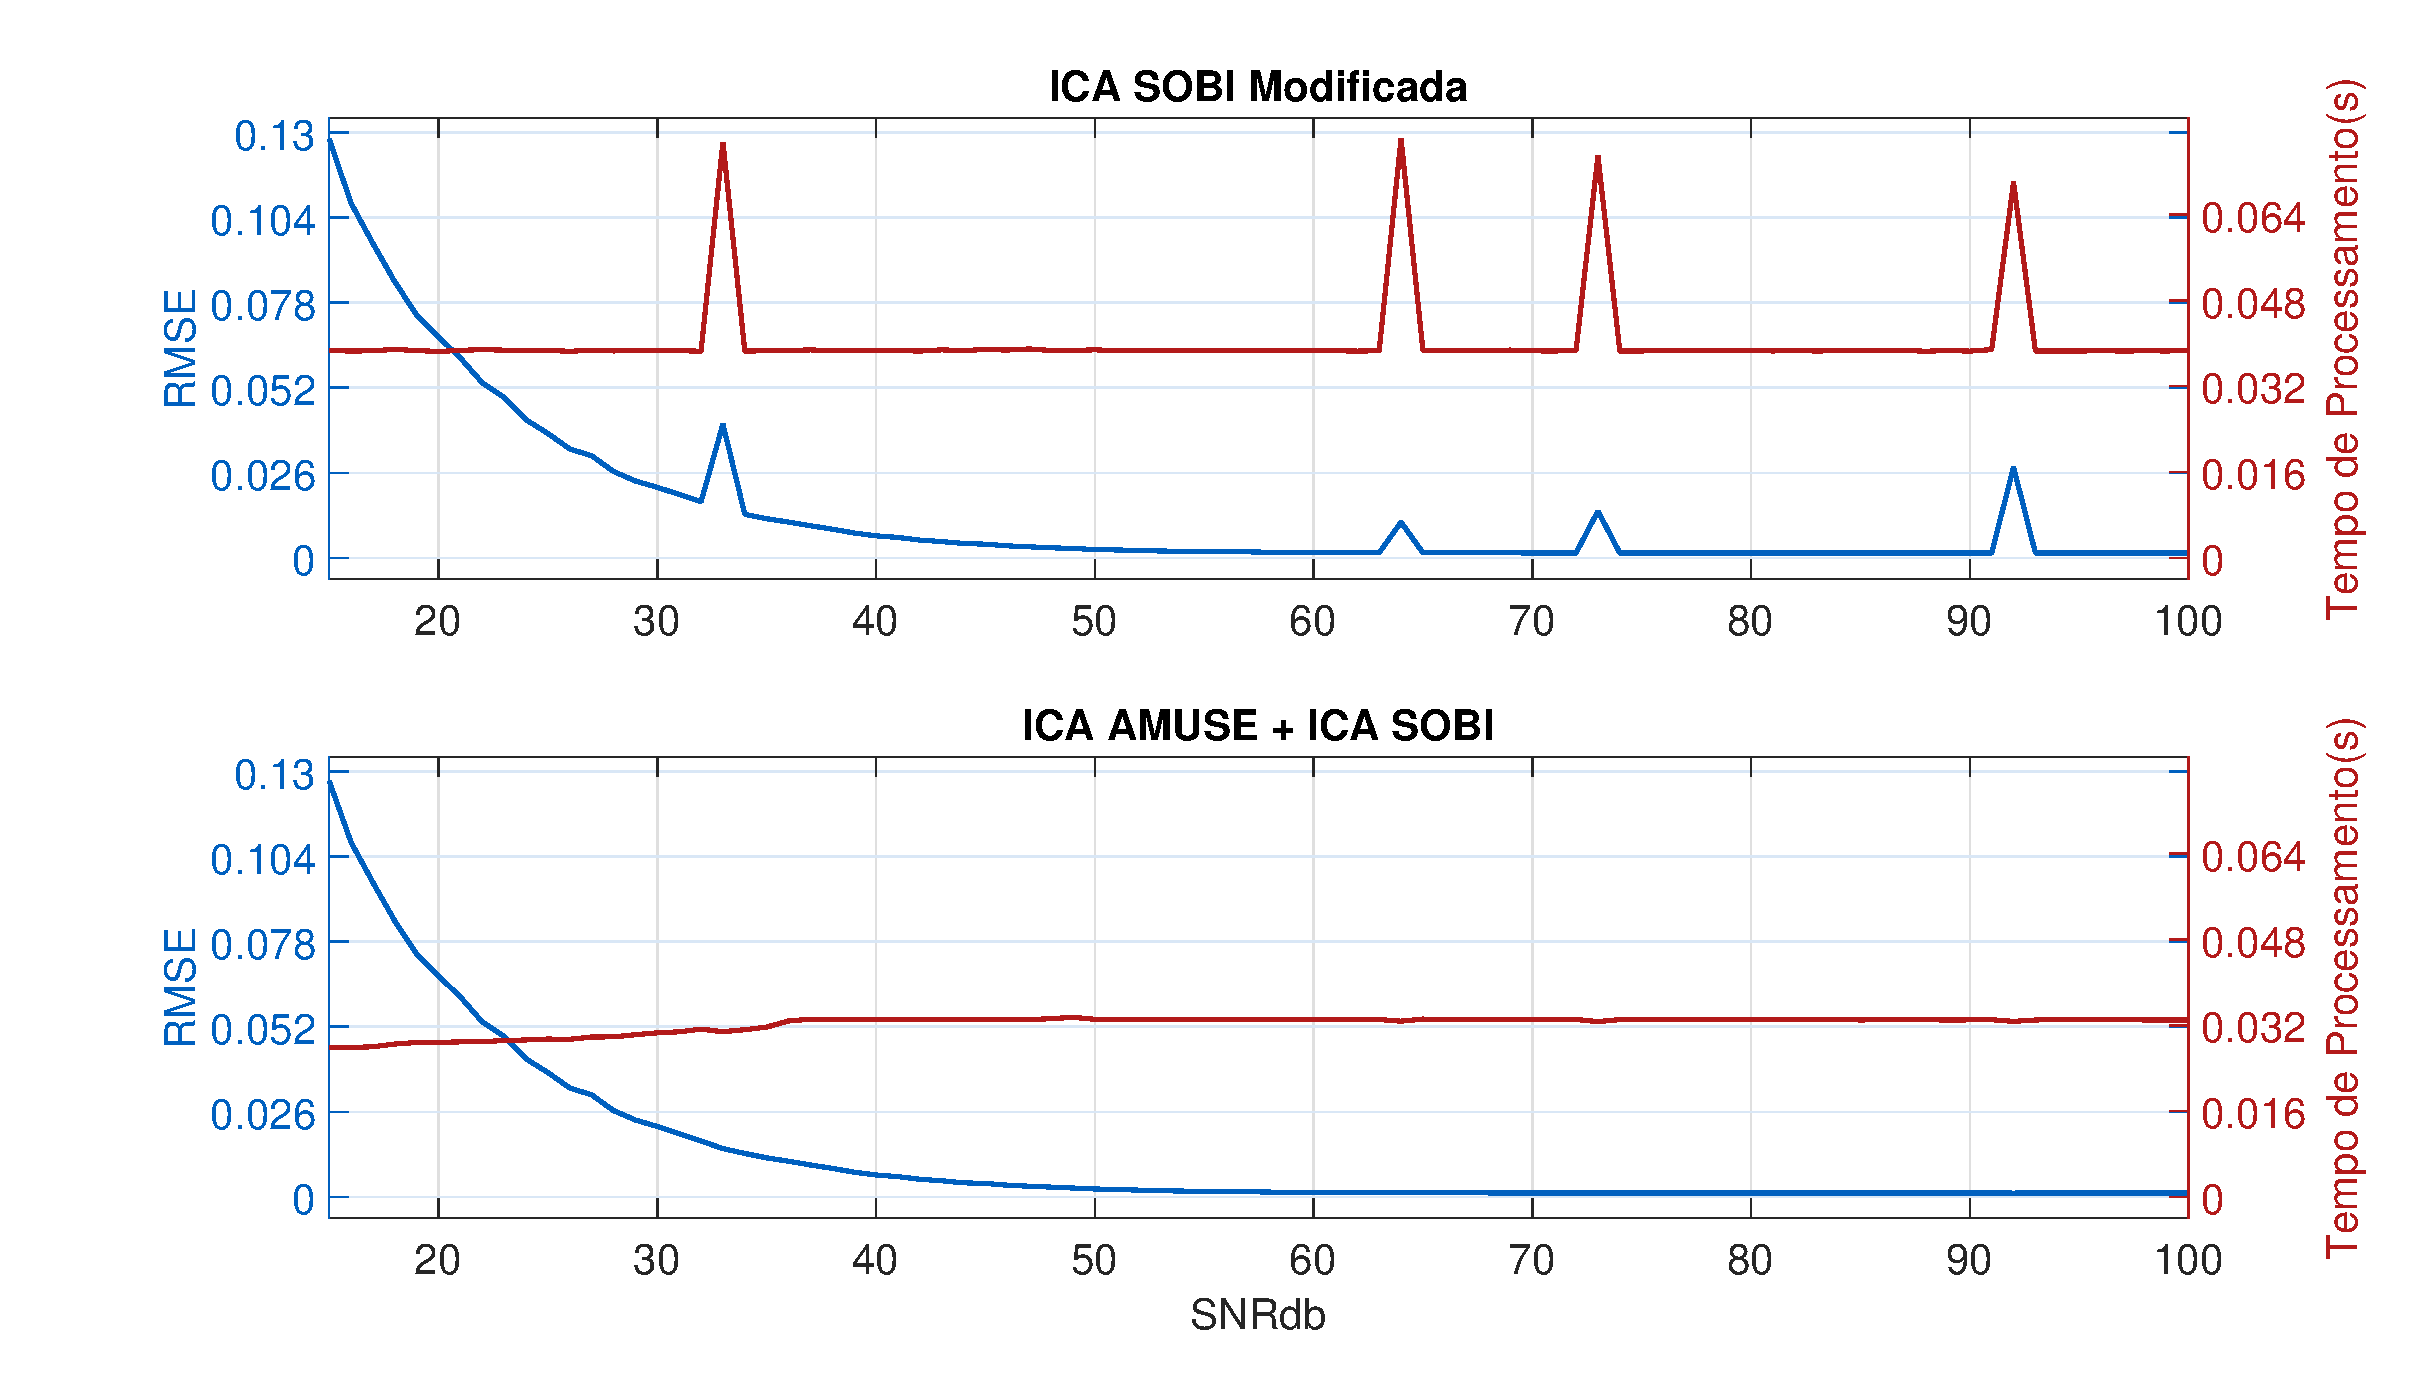
\includegraphics[scale=0.45]{imagens/Sinal5Ruidov2.eps}
    \caption{Resultado da variação do SNRdb para o S5}
    \label{fig:ruidos5}    
    \end{center}
\end{figure}

Analisando-se as Figuras \ref{fig:ruidos1} a \ref{fig:ruidos5}, pode-se perceber que ocorrem picos de $\overline{TP}$ para a ICA SOBI modificada, sendo que isto pode ser devido a pelo menos um de três motivos:
a ICA pode demorar a convergir dependendo da combinação de fases sorteadas; a filtragem feita na recuperação de amplitude pode demorar devido a esta mesma combinação de fases e; a etapa de agrupamento pode demorar a convergir devido ao grande número de componentes independentes.

A soma desses problemas leva o tempo de processamento ($TP$) de um único teste a valores bem mais elevados. Percebe-se que esse fato não ocorre para a combinação de ICAs, devido à redução da matriz de separação $\bf W$ realizada pela ICA AMUSE. Também pode-se destacar que, desconsiderando-se os picos supracitados, o $\overline{TP}$ é praticamente constante e menor que o $TO$ para toda a faixa de valores de SNRdb, ou seja, a relação sinal ruído desde 100~dB até 20~dB pouco influência no  ($\overline{TP}$). Vale destacar também que o maior pico de $\overline{TP}$ ocorreu para o teste do sinal $S3$ (Figura \ref{fig:ruidos3}), chegando próximo a 4.9s. Além disso, percebe-se que no teste do sinal $S1$ (Figura \ref{fig:ruidos1}), bem como nos testes dos sinais $S3$ e $S5$ (Figuras \ref{fig:ruidos3} e \ref{fig:ruidos5}), onde ocorreu pico de $\overline{TP}$ também ocorreu pico de $\overline{RMSE}$. 

Os testes não possuem o mesmo intervalo de variação do SNRdb, pois para valores menores que os apresentados em cada figura, a energia do ruído foi maior ou igual à energia de pelo menos uma das fontes, impossibilitando a separação. Também pode-se notar que o comportamento do $\overline{RMSE}$ é semelhante em todos os gráficos, ou seja, à medida que o SNRdb diminui, o $\overline{RMSE}$ aumenta. Pode-se dizer que a energia do ruído influencia diretamente no $\overline{RMSE}$, ou seja, na qualidade das estimativas. 

\section{Análise de um sinal não estacionário}

Com o intuito de se avaliar o desempenho da solução proposta neste trabalho para estimação dos componentes harmônicos provenientes de um sinal não estacionário que apresenta afundamento de amplitude, foi simulado um conversor AC-DC conectado a uma carga RL ($R = 20\Omega$ e $L  = 25 mH$). Este conversor foi alimentado por uma tensão de 220V com frequência de 60Hz. Utilizou-se uma frequência de amostragem de 15,36 kHz e a simulação foi realizada utilizando-se a plataforma do Simulink/Matlab.

Com o objetivo de obter o afundamento de amplitude, em um determinado momento da simulação foi alterado o ângulo de disparo do conversor AC-DC ($ \alpha $). Seu valor inicialmente era $ \alpha = 10^{\circ}$ e passou a valer $ \alpha = 80^{\circ}$, o que ocasionou uma alteração nas amplitudes das componentes do sinal de corrente do conversor. Para estimar a componente fundamental do sinal, foi utilizada a Transformada Discreta de Fourier em Janela, também denominada de Transformada Discreta de Fourier Recursiva (DFT Recursiva). Neste trabalho, foi utilizada uma janela retangular com tamanho igual a 256 amostras, ou seja, um ciclo da fundamental. 

Como nesta simulação a frequência da fundamental se mantém constante, a DFT Recursiva não sofre de espalhamento espectral, de forma que o rastreamento em regime permanente é exato. Na Figura \ref{fig:sinalafundado1}, tem-se o sinal simulado bem como a estimação da fundamental dada pela DFT Recursiva. Vale destacar que aproximadamente na metade do sinal ocorre o afundamento na sua amplitude. Também pode-se notar que antes do afundamento, a fundamental estimada tem amplitude mais elevada que a do sinal.

\begin{figure}[!htb]
    \begin{center}
    \advance\leftskip -1.5cm
    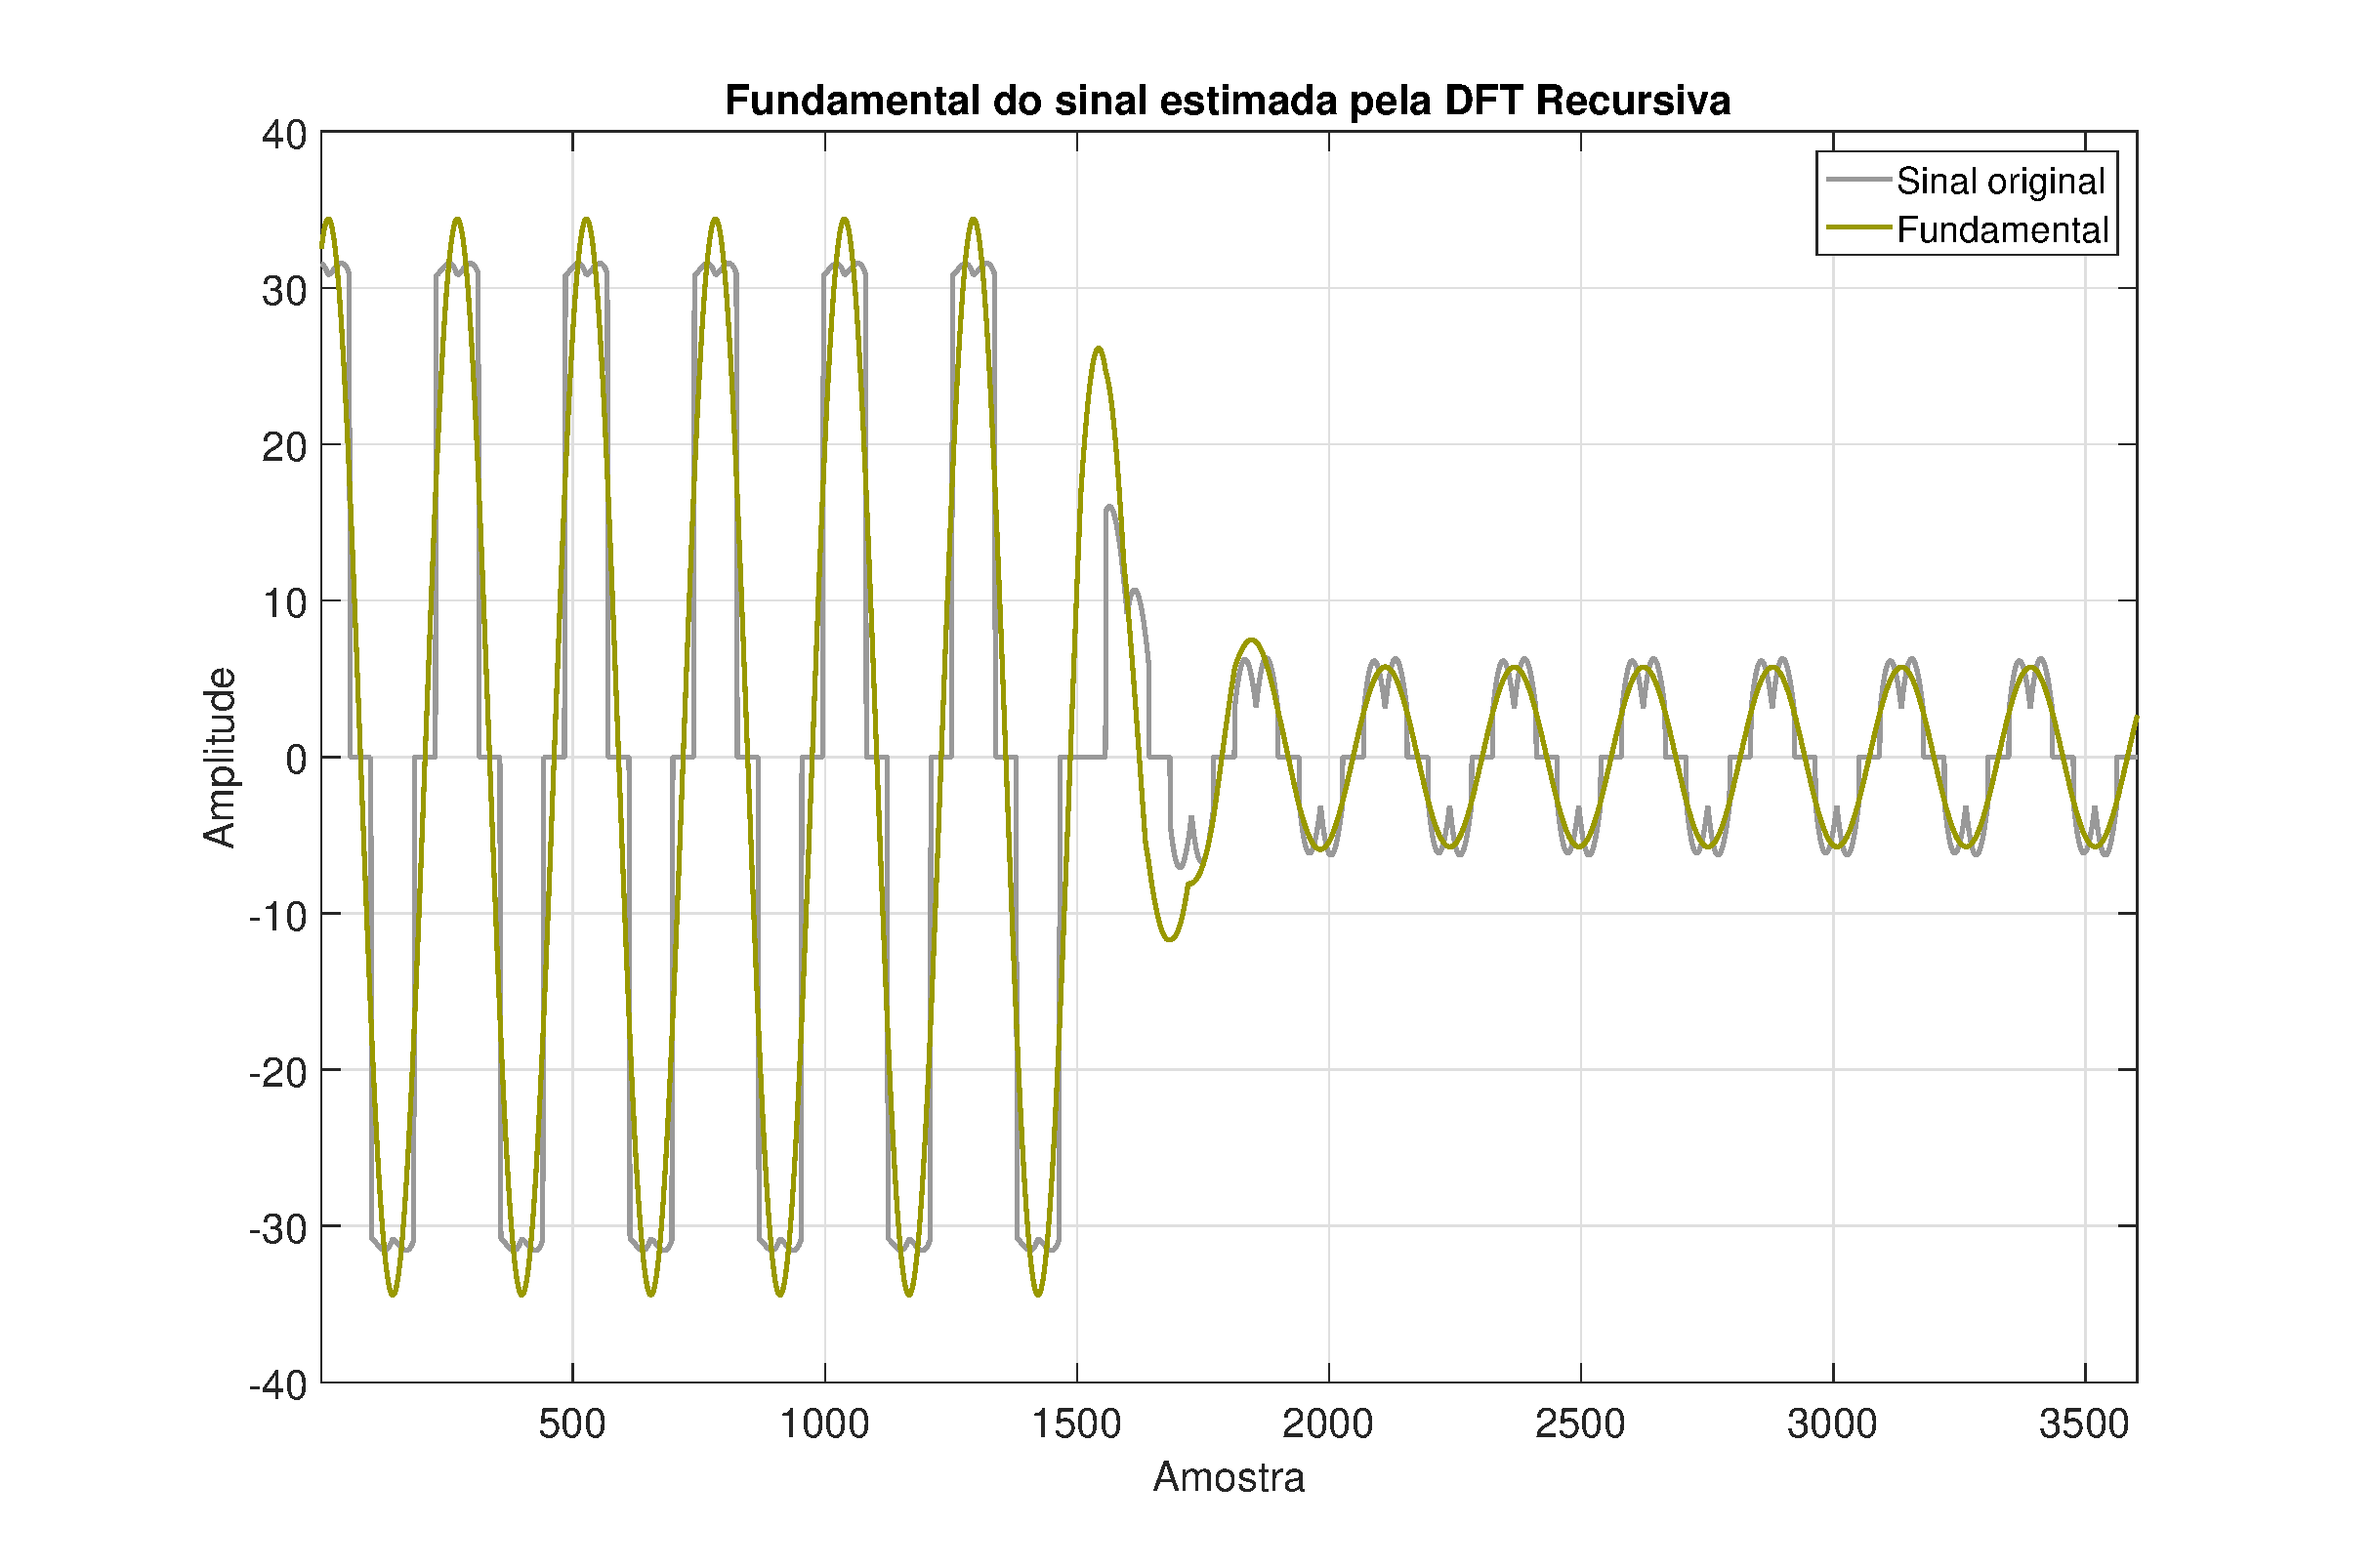
\includegraphics[scale=0.41]{imagens/PlotSinal.eps}
    \caption{Sinal de entrada e sua componente fundamental estimada.}
    \label{fig:sinalafundado1}    
    \end{center}
\end{figure}

Após a estimação da fundamental, foi utilizado o sistema proposto neste trabalho, empregando todas as quatro ICAs analisadas. Os resultados para a estimação da fundamental podem ser vistos na Figura \ref{fig:sinalafundado2} e na Tabela \ref{tab:sinalaundado}. A Figura \label{fig:sinalafundado2}  mostra a estimativa da fundamental para cada ICA testada, na qual pode-se perceber que quando o sinal de entrada se encontra em um regime quase-estacionário, a diferença entre a estimação dada pela DFT Recursiva e por todos os algoritmos de ICA é baixa, por se dizer praticamente nula, exceto para a região próxima à transição de amplitude, onde os algoritmos de ICA divergem da estimação realizada pela DFT Recursiva. Isto se deve à natureza da DFT Recursiva, que apresenta períodos transitórios para estabilização, o que não ocorre na ICA. Analisando-se a Tabela \ref{tab:sinalaundado}, tem-se que apenas a ICA AMUSE e a Combinação de ICAs possuem $TP$ menor que o $TO$ do sinal.

\begin{figure}[!htb]
    \begin{center}
    \advance\leftskip -1.5cm
    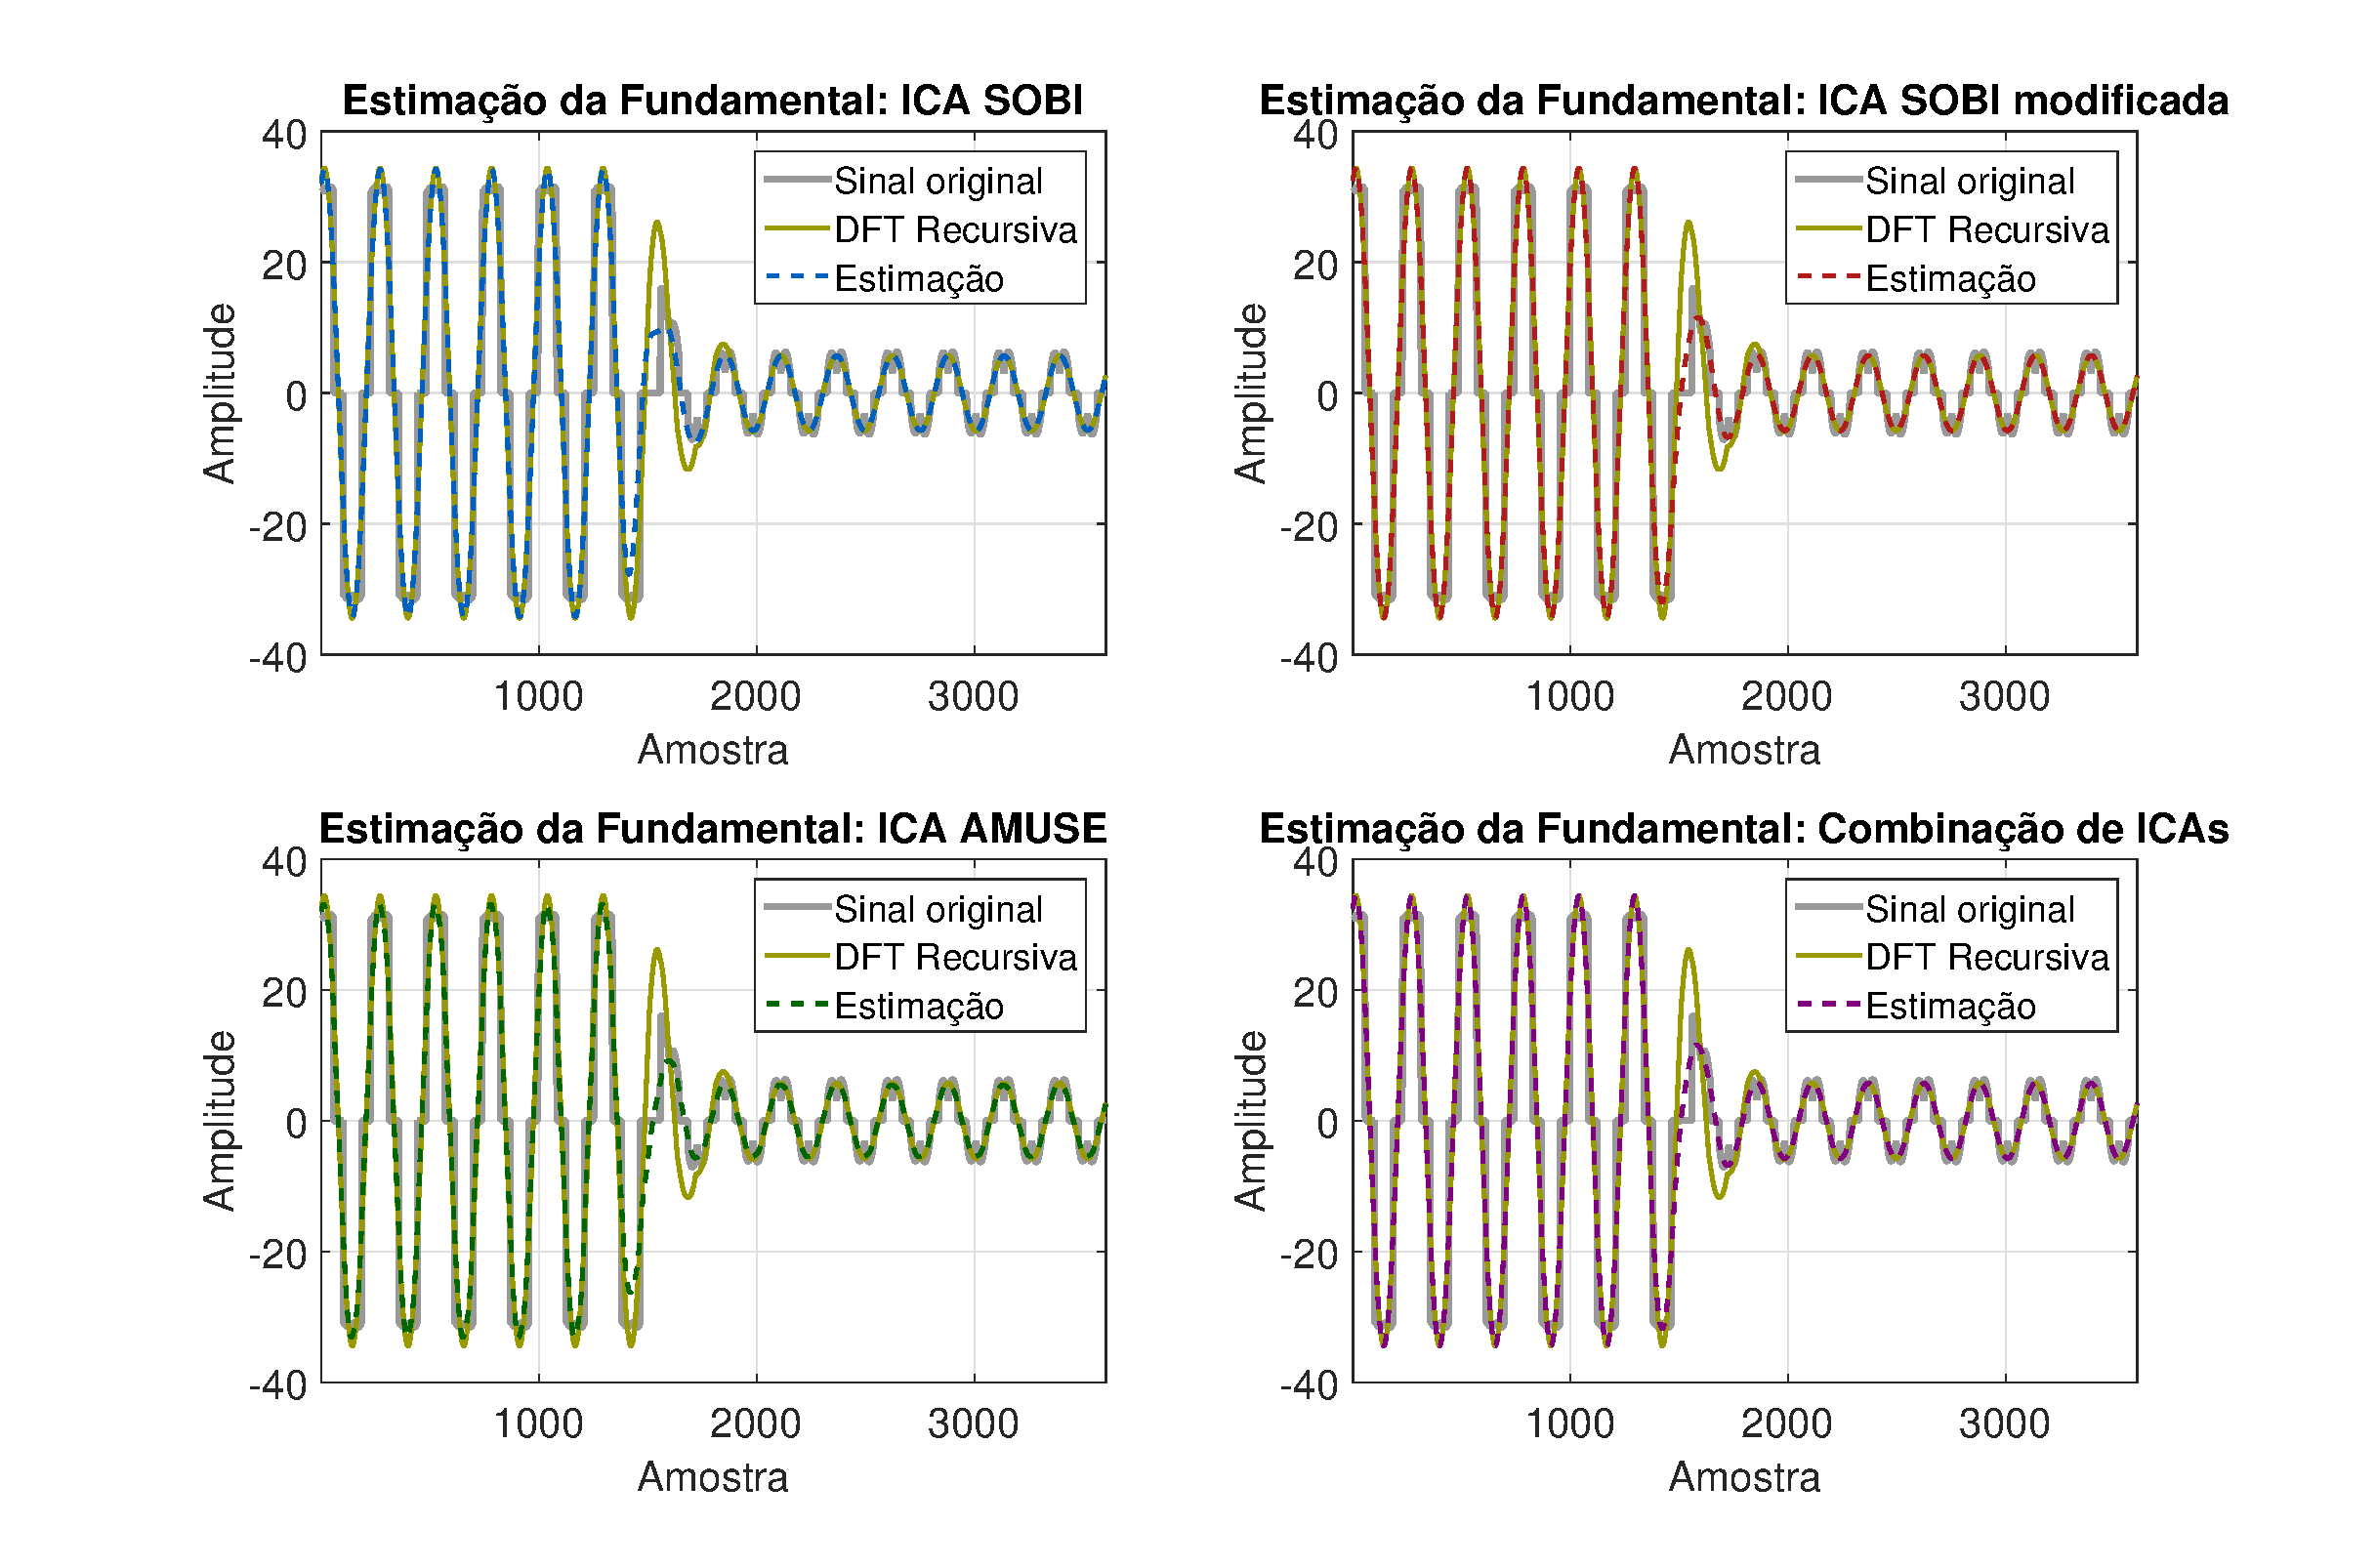
\includegraphics[scale=0.41]{imagens/PlotFundsEstimadas.eps}
    \caption{Componente fundamental estimada por cada ICA.}
    \label{fig:sinalafundado2}    
    \end{center}
\end{figure}

\begin{table}[!htb]
    \begin{center}
        \caption{Tempo de Processamento para estimação dos componentes do sinal não estacionário.}
        \begin{tabular}{c|c c c c c}
        \hline
        ICA & SOBI & SOBI mod & AMUSE & Combinação & $TO$ (s)\\ 
        \hline
        $TP$ (s) & 55.438 & 0.697 & 0.147 & 0.239 & 0.260\\
        \end{tabular}
        \label{tab:sinalaundado}
    \end{center}
\end{table}

Para enfatizar melhor a diferença entre a estimação dada pela DFT Recursiva e pelas ICAs, tem-se o resultado da Figura \ref{fig:sinalafundado3}. Nela, tem-se a estimação da fundamental em azul, e em vermelho e verde tem-se estimações de distúrbios transitórios. O interessante de se notar é que os distúrbios começam antes da ocorrência do afundamento do sinal, e o mesmo ocorre com a estimação da fundamental. Ao comparar as Figuras \ref{fig:sinalafundado1}  e \ref{fig:sinalafundado3}, nota-se também que no método da DFT Recursiva o afundamento da fundamental estimada se inicia pouco antes do afundamento do sinal, gerando uma pequena deformação da fundamental. A mesma deformação não é vista na Figura \ref{fig:sinalafundado3}.

\begin{figure}[!htb]
    \begin{center}
    \advance\leftskip -1.5cm
    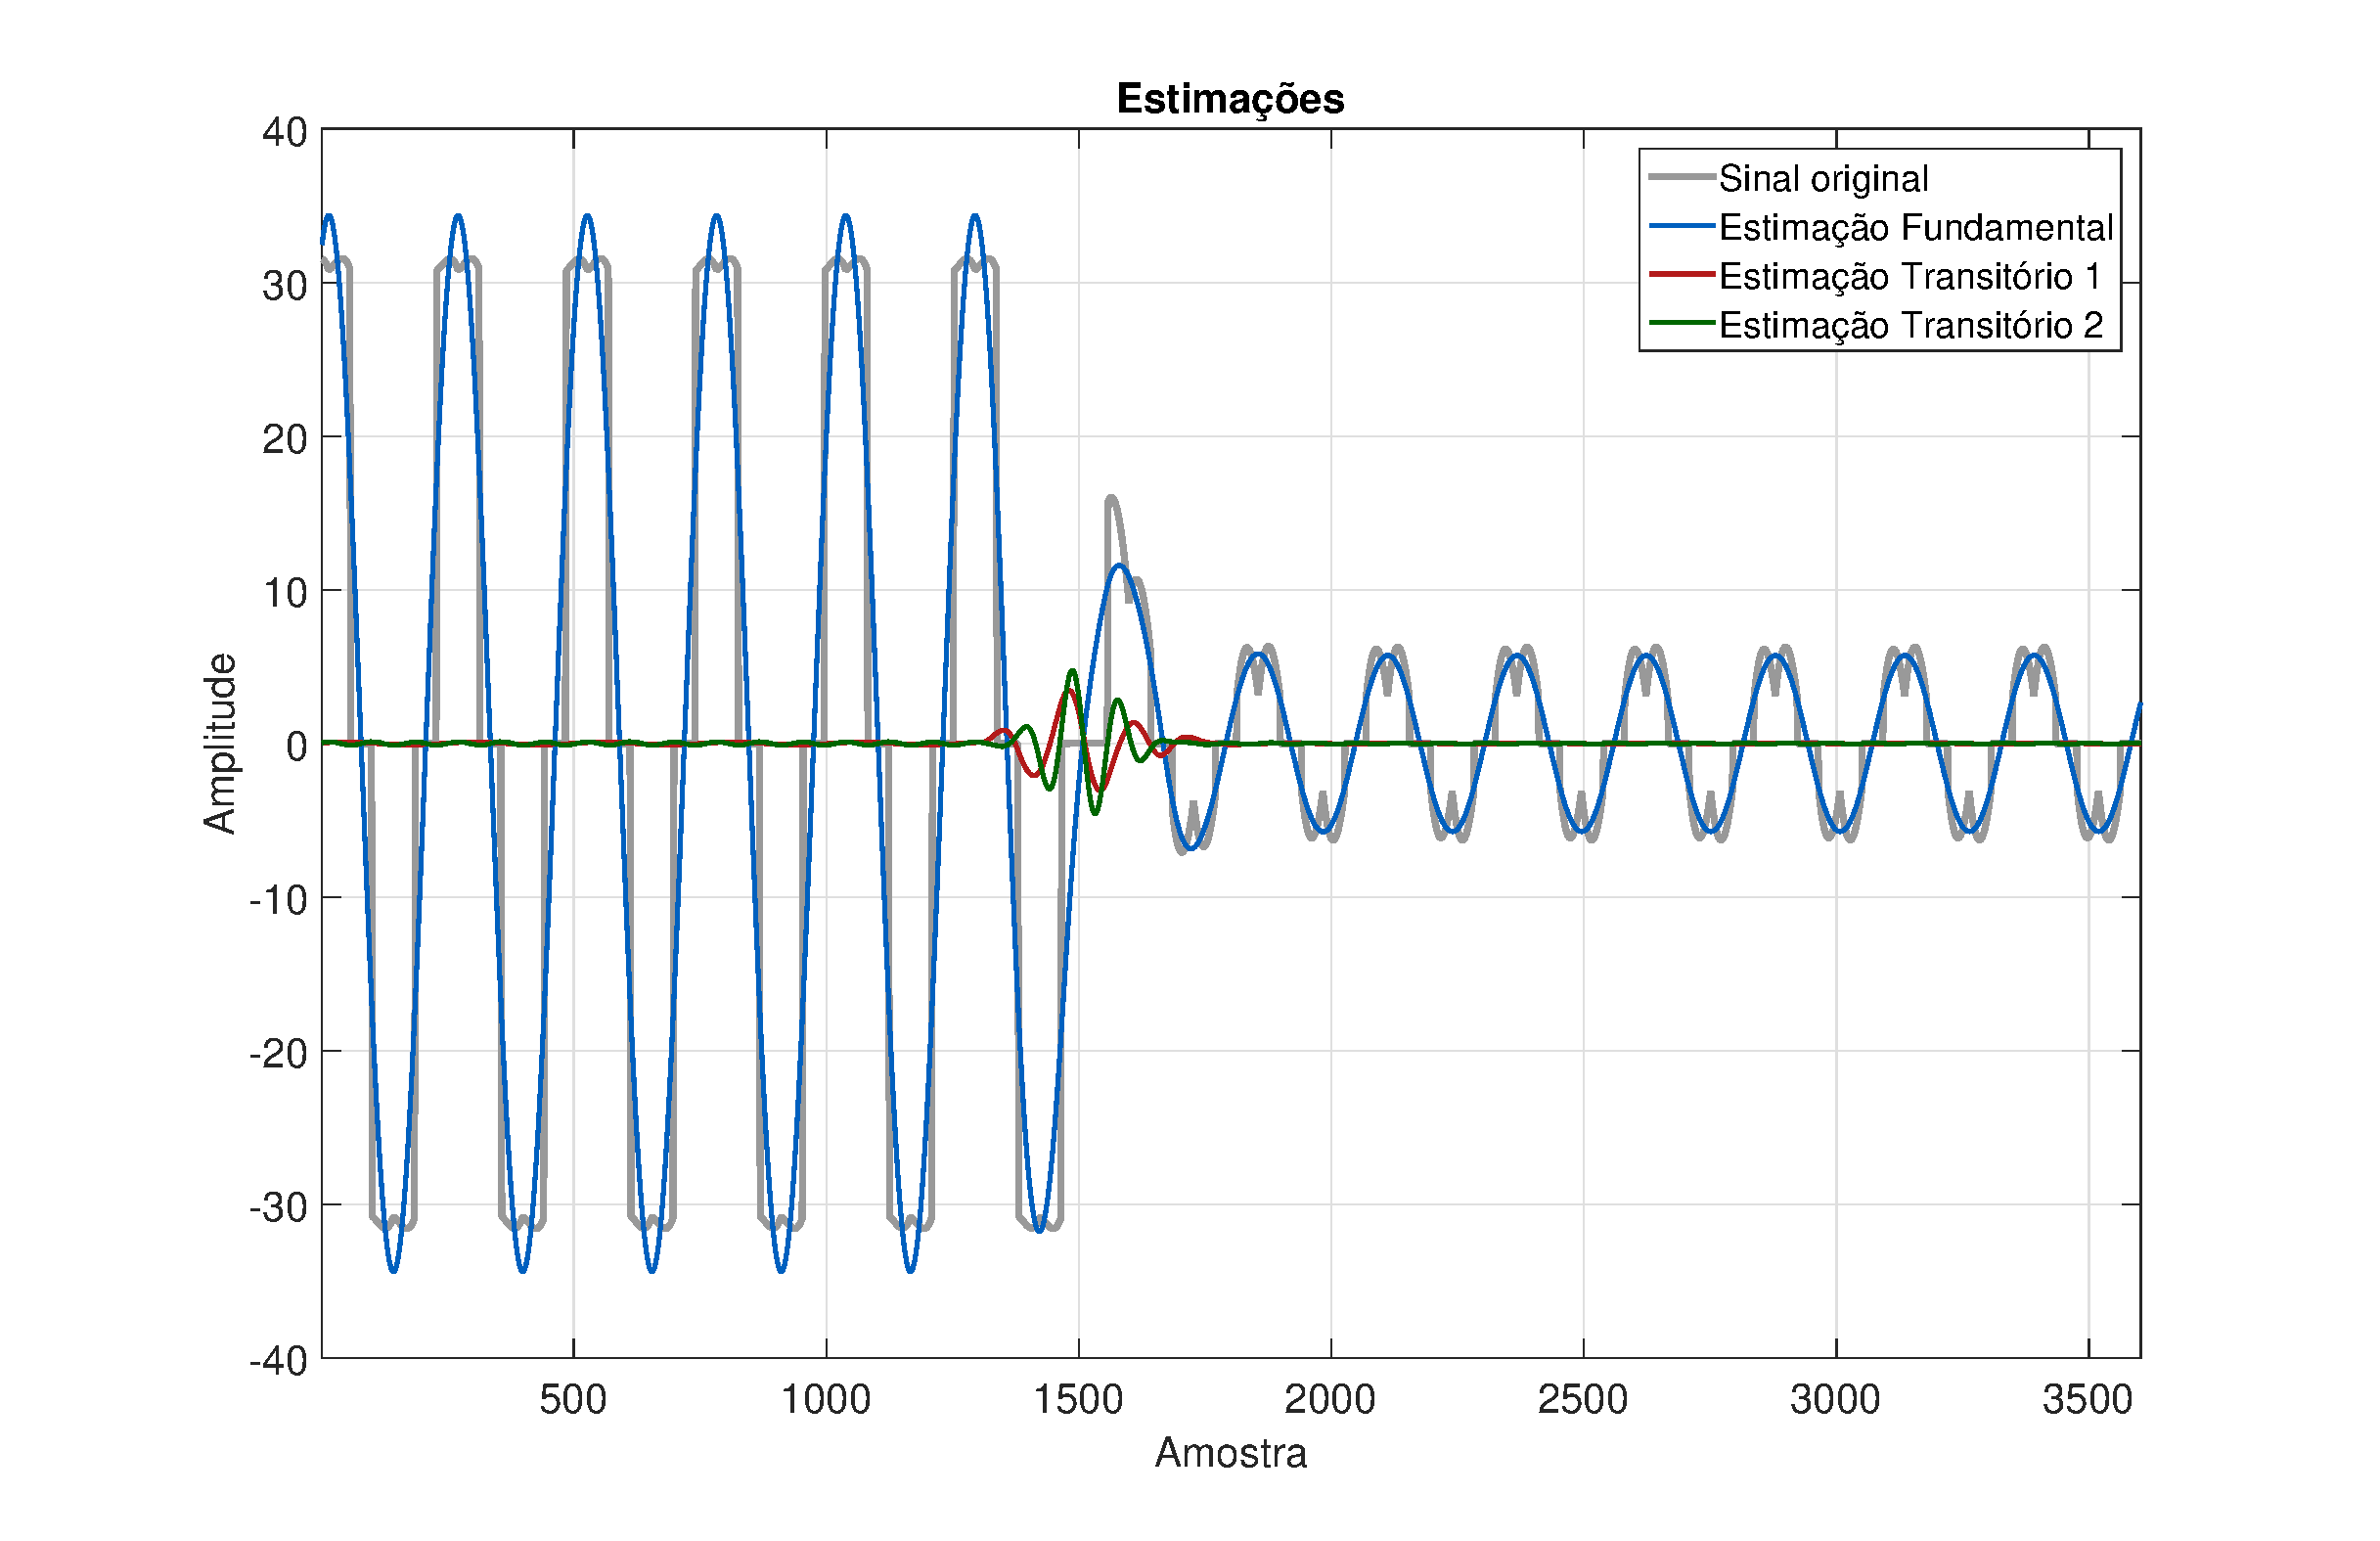
\includegraphics[scale=0.41]{imagens/Estimacoes.eps}
    \caption{Estimações realizadas pela ICA.}
    \label{fig:sinalafundado3}    
    \end{center}
\end{figure}

Assim, pode-se concluir que a estimação realizada pelo método proposto, durante o afundamento, é mais exata do que a estimação realizada pela DFT Recursiva. Isto se deve à capacidade da ICA de estimar outras formas de distúrbios de qualidade de energia, além do distúrbio harmônico. Deve-se deixar claro que as estimativas dos demais componentes harmônicos não foram mostradas por possuirem resultados semelhantes.

\chapter{CONCLUSÃO}
\label{ch:conclusao}

Tendo-se em vista o objetivo deste trabalho, que é estimação de componentes harmônicos e inter-harmônicos, o sistema proposto de modo geral demonstrou eficiência tanto na estimação quanto com relação ao tempo de processamento.

Ao analisar os algoritmos de ICA, pode-se dizer que a ICA SOBI sem modificações possui um tempo de processamento muito elevado, bem como um erro quadrático médio normalizado mais elevado que as demais ICAs. Também pode-se dizer que a ICA AMUSE, apesar do bom tempo de processamento, assim como a ICA SOBI sem as modificações, possui um erro quadrático médio elevado. Assim, pode-se concluir que as modificações realizadas na ICA SOBI e a combinação de ICAs apresentaram melhores resultados tanto com relação ao tempo de processamento quanto em relação ao erro quadrático médio normalizado.

Ao analisar o comportamento do sistema de acordo com o número de atrasos $m$, pode-se concluir que, em geral, o tempo de processamento aumenta à medida que o número de atrasos aumenta. Entretanto, o mesmo sempre é menor que o tempo de obtenção do sinal, salvo pequenas exceções. Também tem-se que o erro quadrático médio normalizado tende a resultar em uma boa estimação para um número de atrasos em torno de $N_s/5$. Porém, nem sempre esse valor é viável, visto que o tamanho do sinal e o número de atrasos têm grande peso no tempo de processamento. 

Analisando o sistema de acordo a variação da relação sinal ruído, tem-se que o tempo de processamento permanece constante salvo pequenas exceções, e o mesmo se mantém menor que o tempo de obtenção do sinal. Assim, o tempo de processamento é praticamente indiferente em relação à variação da relação sinal ruído. Tem-se também que o erro quadrático médio normalizado possui valores mais elevados à medida que a relação sinal ruído diminui.

Conclui-se também que ao utilizar o sistema proposto para um sinal não estacionário, o método tem um bom comportamento, estimando inclusive os distúrbios transitórios do sinal.

Por fim, ao analisar o trabalho como um todo, pode-se concluir que a combinação proposta de ICAs AMUSE e SOBI Modificada possui o melhor desempenho em todos os aspectos observados, seja em termos do $RMSE$ ou do $TP$. Deste modo, a utilização deste método hibrido auxiliado com o algoritmo EMO diminui substancialmente o custo computacional, viabilizando, inclusive, a separação \textit{online} em janelas.  


%%%%%%%%%%%%%%%%%%%%%%%%%%%%%%%%%%%%%%%
\singlespacing
\bibliographystyle{abntex2-alf}
\bibliography{referencias}
%%%%%%%%%%%%%%%%%%%%%%%%%%%%%%%%%%%%%%%%%%%%%%%%

\appendix
\chapter{Resultados adicionais}

Este apêndice tem o intuito de mostrar os gráficos de resultados de testes adicionais, omitidos no texto para que o mesmo não se tornasse demasiadamente longo.

\section{Testes Sucessivos}

As Figuras de A.1 até A.6 apresentam os resultados adicionais obtidos para um sinal com quatro componentes, cujo modelo se encontra na Tabela \ref{tab:sorteio}. Já as Figuras de A.7 até A.12 são os resultados adicionais obtidos para um sinal com oito componentes, cujo modelo se encontra na Tabela \ref{tab:sorteioc}. As conclusões a respeito da análise desses sinais podem ser vistas no seção \ref{ch:testesus}.

\section{Sensibilidade ao Número de Atrasos}

Nesta Seção, são apresentados os resultados extras obtidos para os testes de variação do número de atrasos $m$ do bloco atrasador do método proposto. Esses resultados foram obtidos a partir da análise dos sinais cujos modelos são apresentados na Tabela \ref{tab:Sinais}. Vale destacar que o tempo de processamento do método aumenta progressivamente com o aumento do número de atrasos.
Também se dá destaque ao fato de que o componente com maior $RMSE$ praticamente modela o comportamento da curva do $RMSE$ médio, ou seja, quando se analisa a forma da curva, os componentes com baixo $RMSE$ possuem pouca importância. As Figuras A.13 até A.27 apresentam esses resultados.

\section{Sensibilidade ao Ruído}

Nesta Seção, são apresentados os resultados extras obtidos para os testes de variação da relação sinal ruído (SNRdb). Vale destacar que não há alteração no tempo de processamento em função da variação da SNRdb. Assim, mesmo nos casos de pico de tempo de processamento citados na seção \ref{ch:testeRU} deste trabalho, todos os blocos demoram por igual para serem executados à medida que a SNRdb varia.
Também se dá destaque ao fato de que o componente com maior $RMSE$ normalmente é o componente com mais baixa amplitude. As Figuras A.28 até A.42 apresentam esses resultados.

\begin{figure}[!htb]
    \begin{center}
    \advance\leftskip -1.5cm
    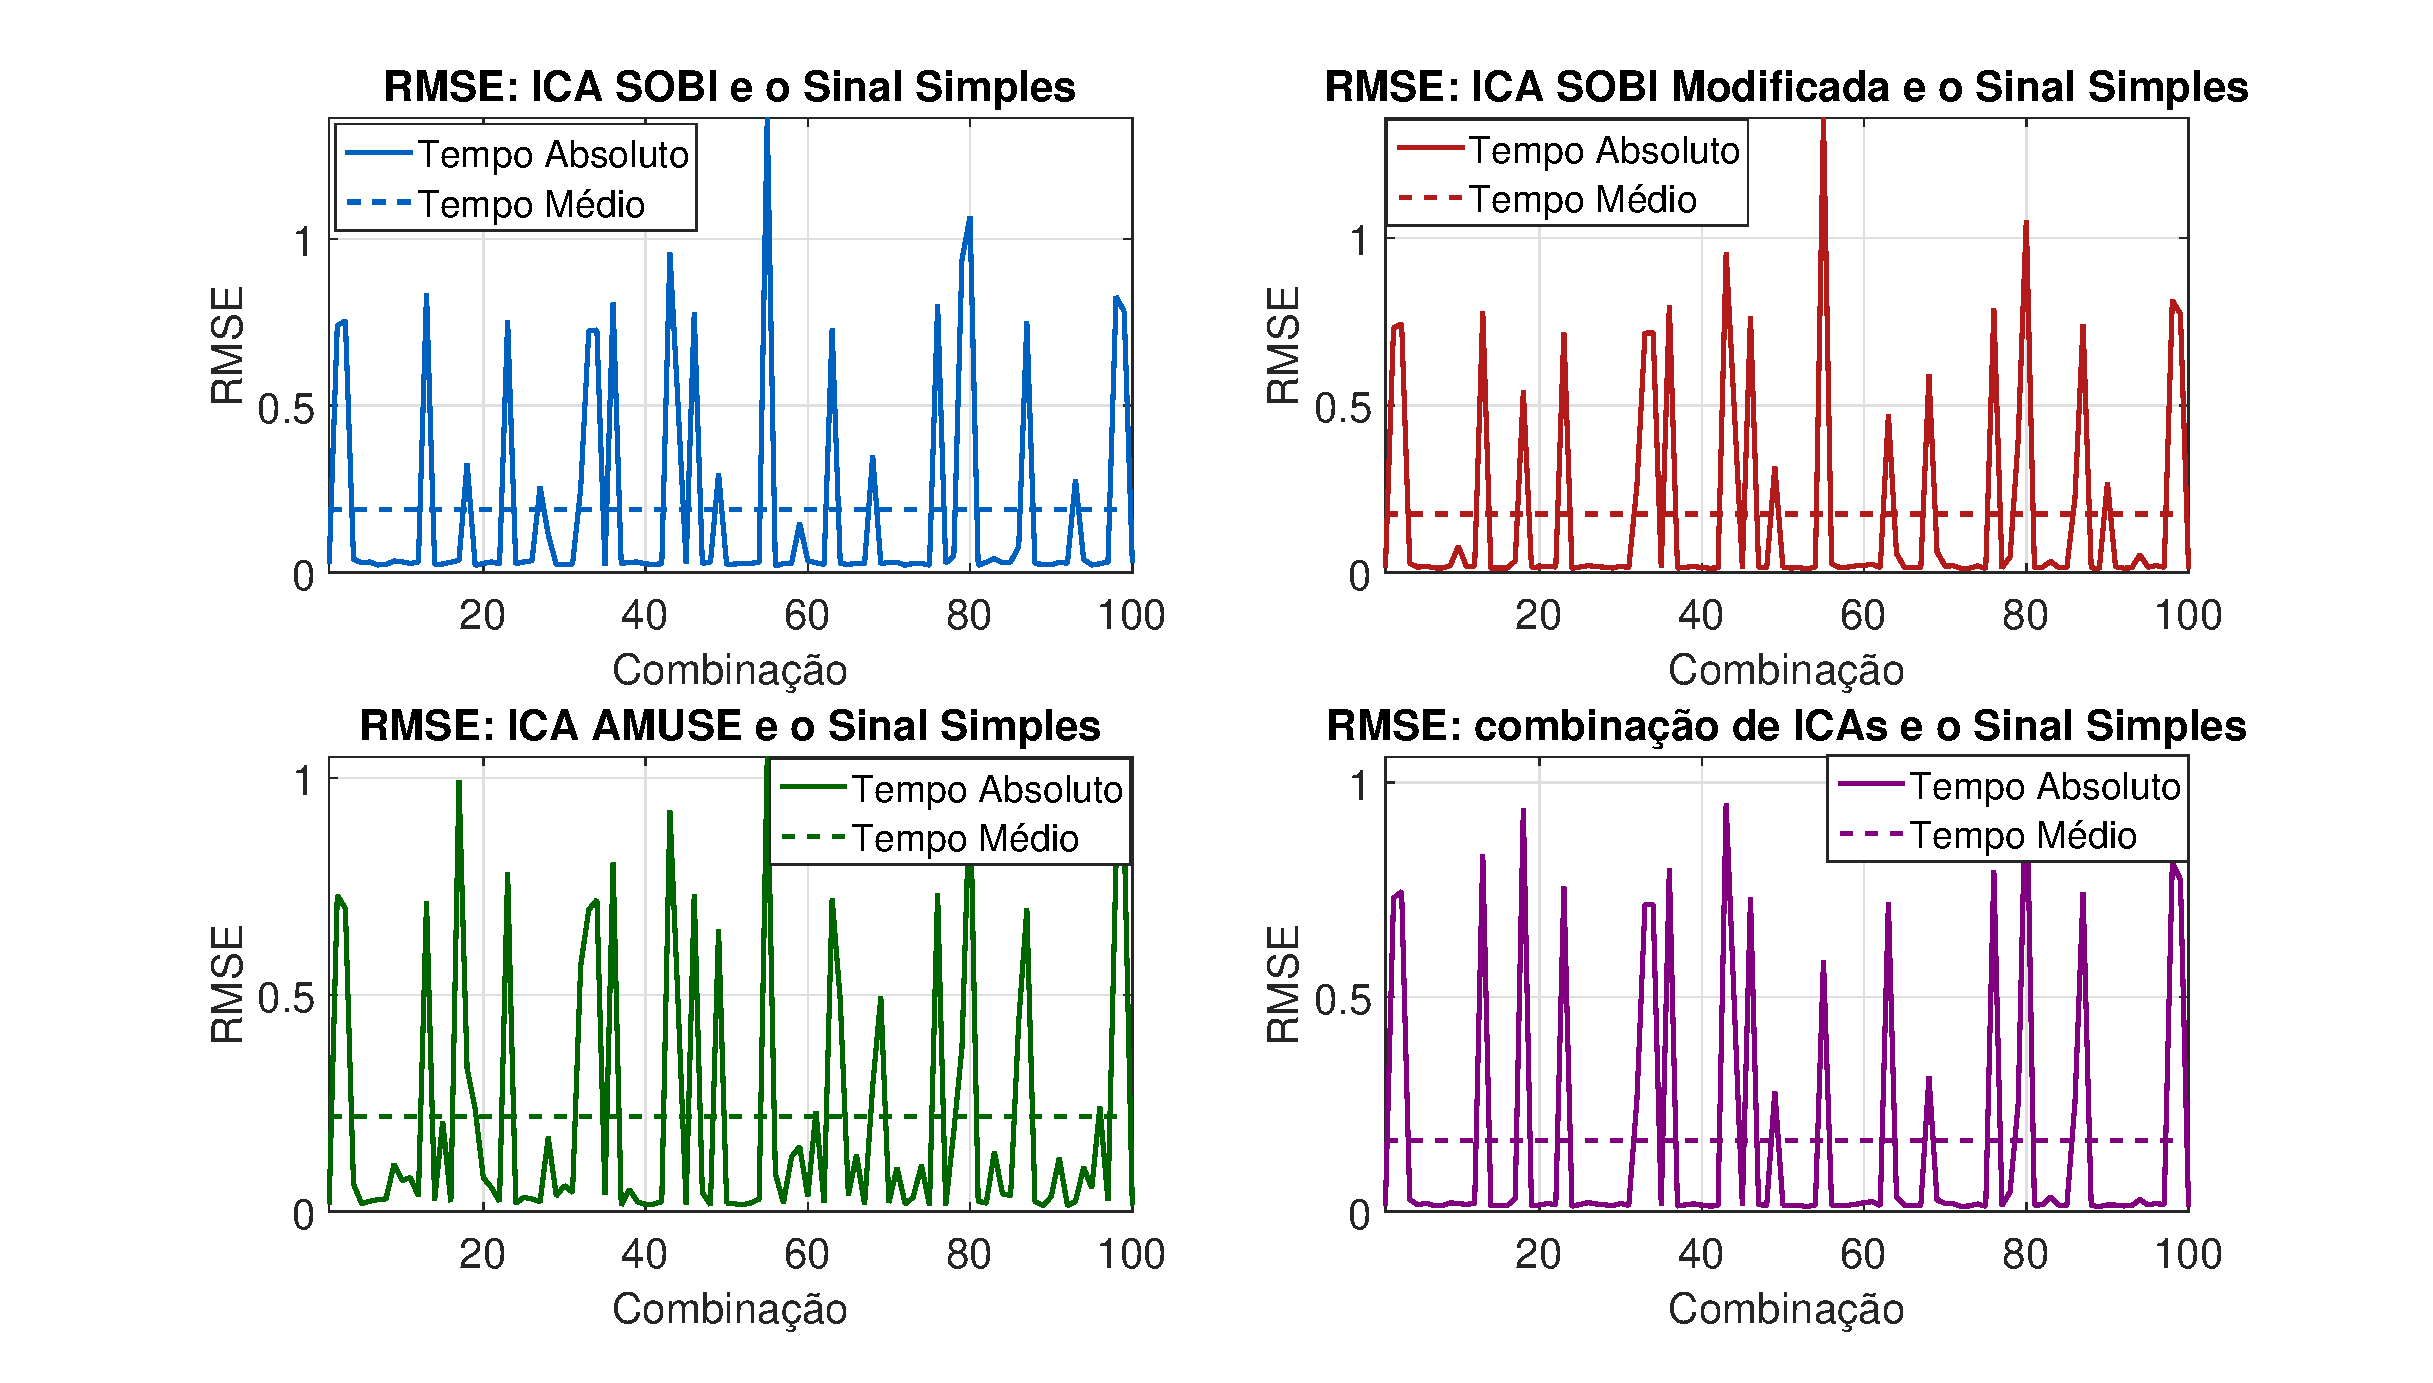
\includegraphics[scale=0.45]{imagens/ImagensParaOAnexo/RMSEETodasICAsSinalSimples.eps}
    \caption{RMSE de todos os testes e todas as ICAs para um sinal com quatro componentes.}
    \label{fig:RMSESinalsimples}    
    \end{center}
\end{figure}

\begin{figure}[!htb]
    \begin{center}
    \advance\leftskip -1.5cm
    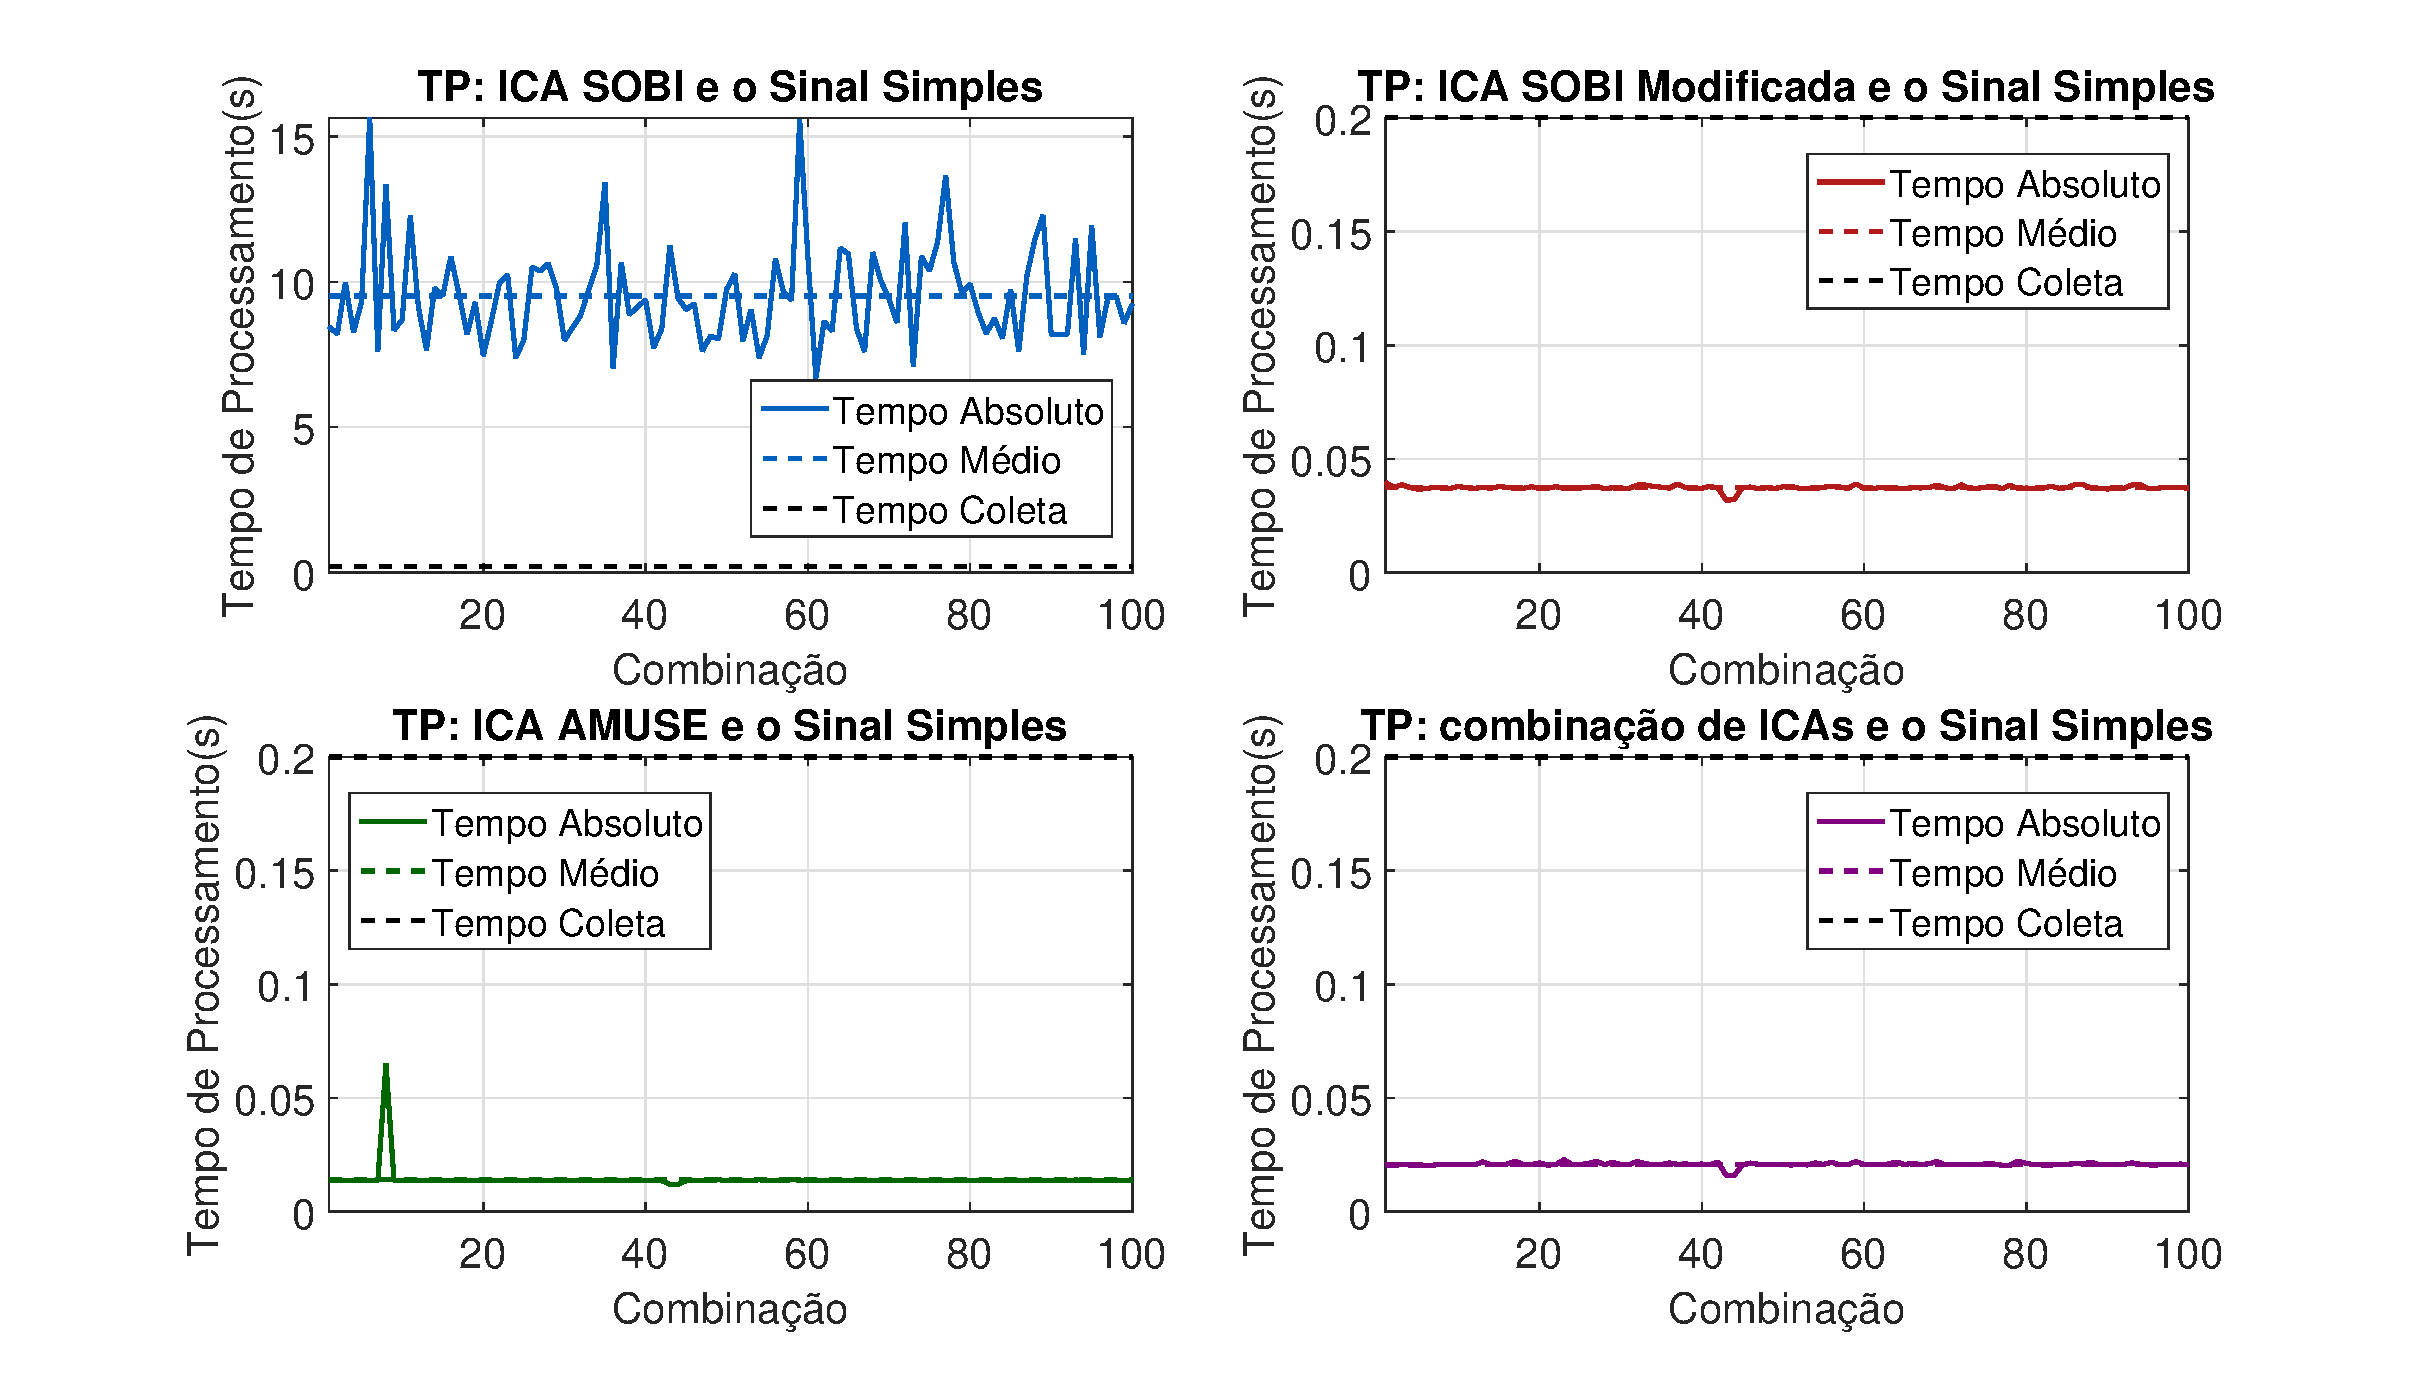
\includegraphics[scale=0.45]{imagens/ImagensParaOAnexo/TPAETodasICAsSinalSimples.eps}
    \caption{TP de todos os testes e todas as ICAs para um sinal com quatro componentes.}
    \label{fig:TPSinalsimples}    
    \end{center}
\end{figure}

\begin{figure}[!htb]
    \begin{center}
    \advance\leftskip -1.5cm
    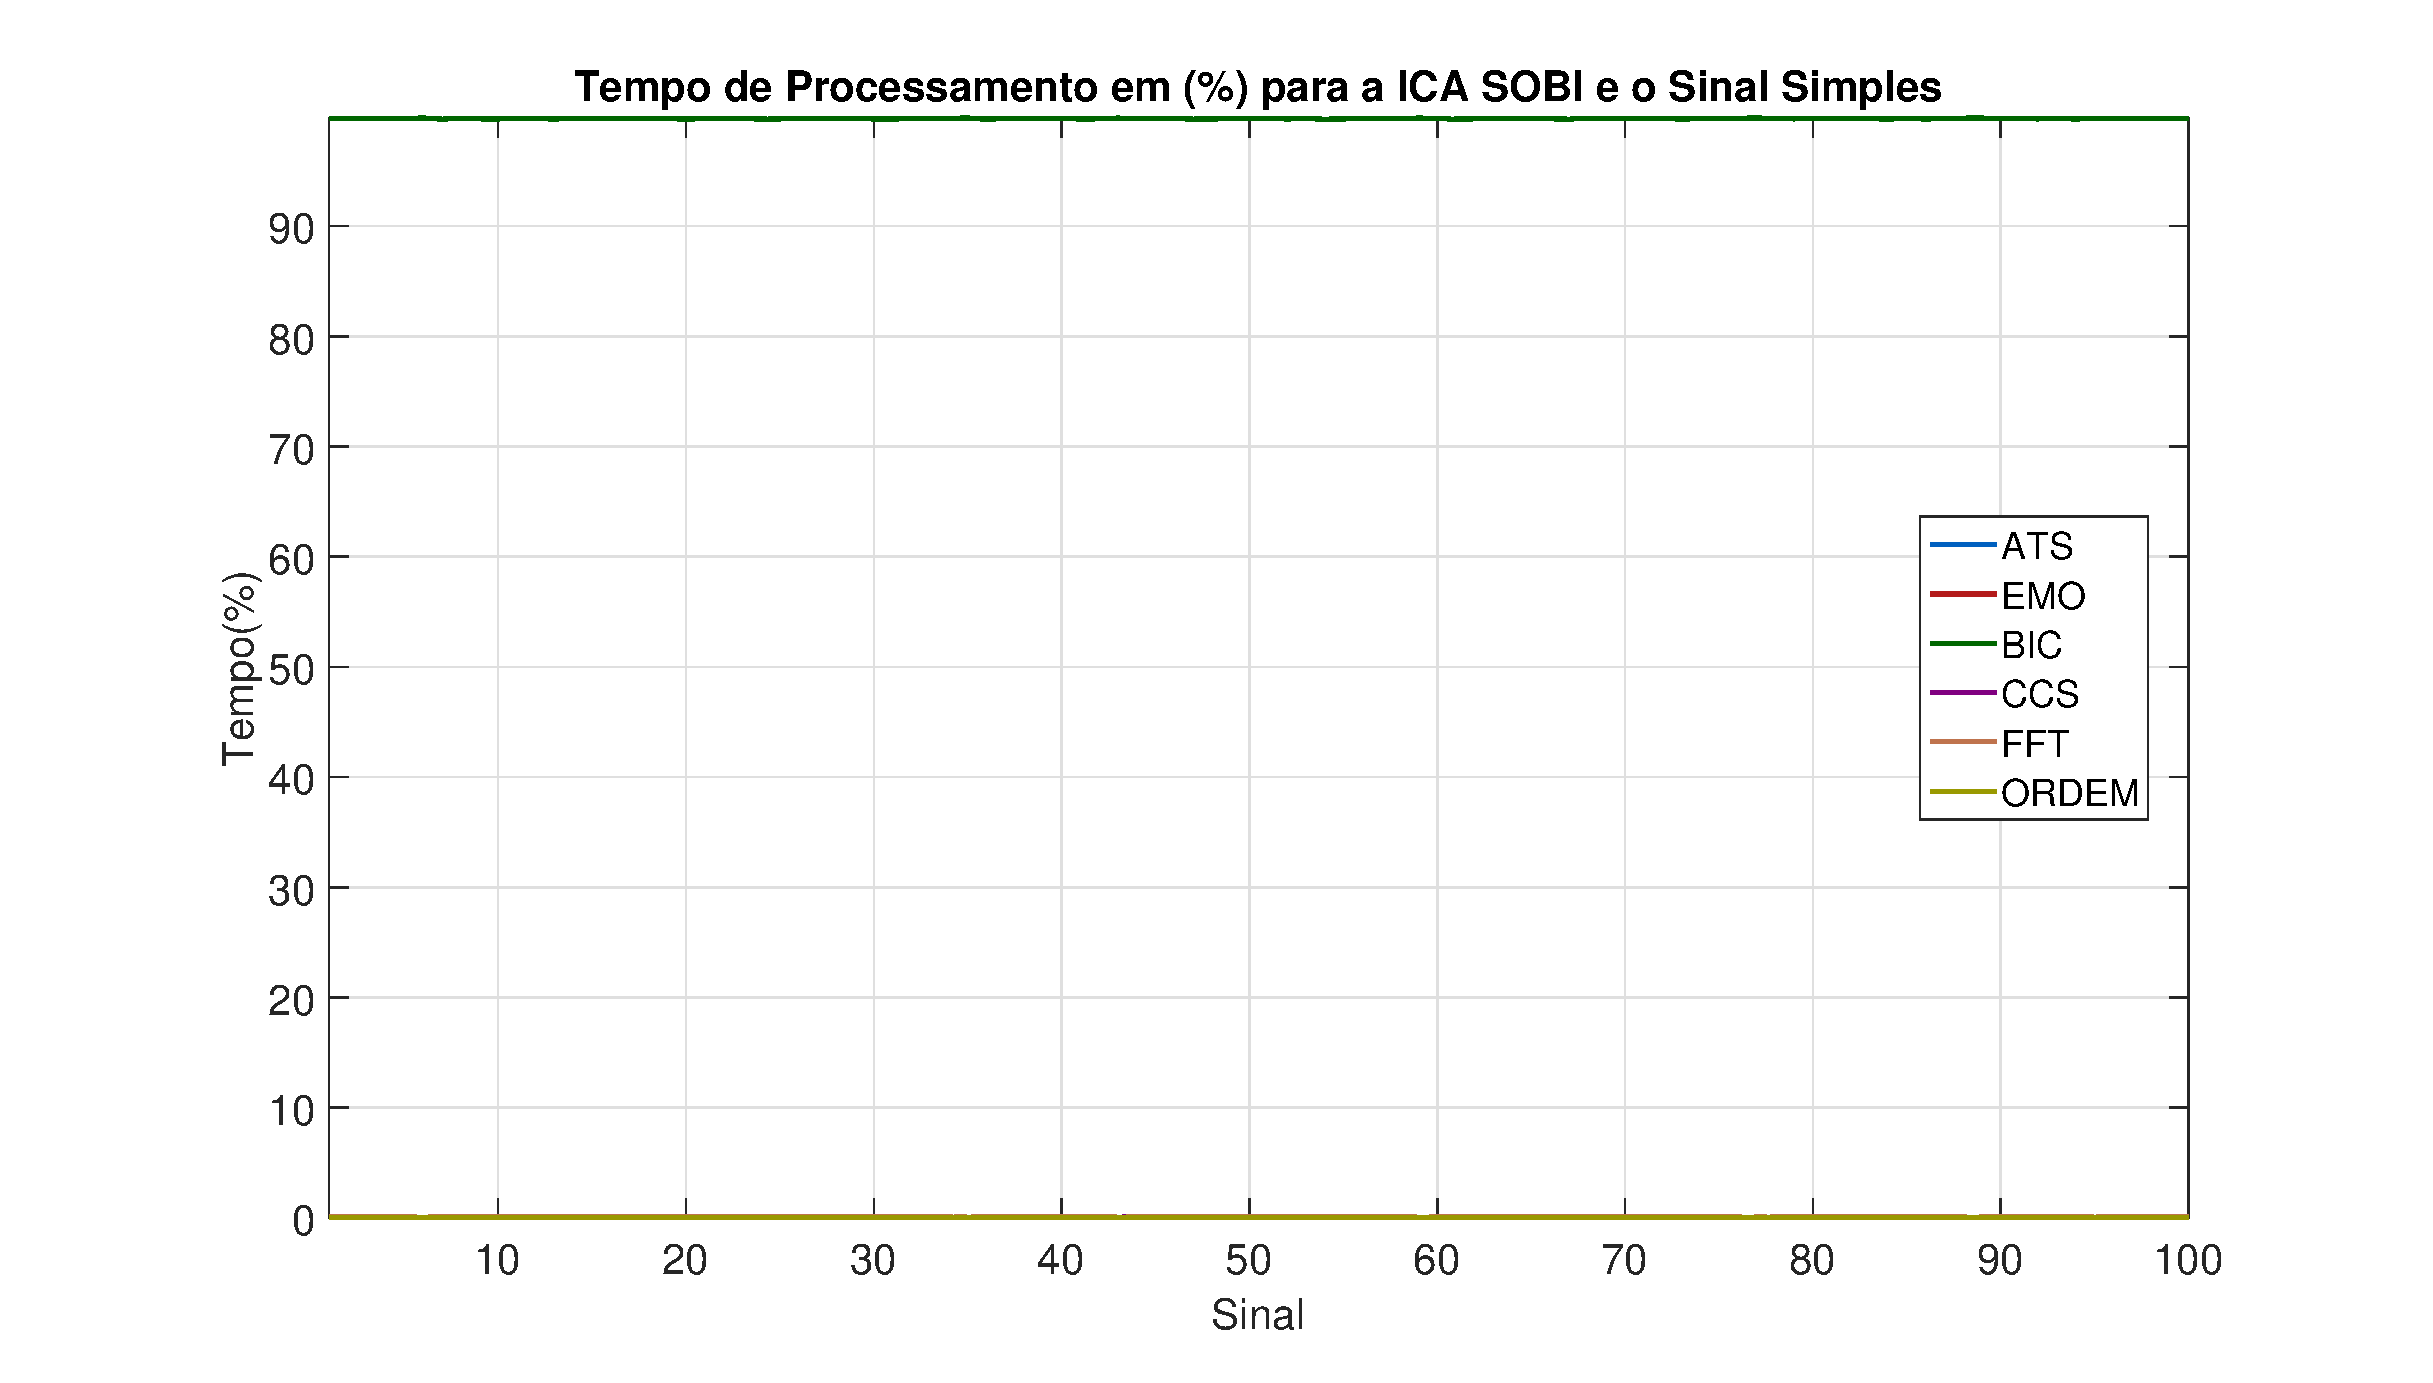
\includegraphics[scale=0.45]{imagens/ImagensParaOAnexo/TPPEICASOBISinalSimples.eps}
    \caption{TP em porcentagem de todos os testes para ICA SOBI e um sinal com quatro componentes.}
    \label{fig:TPSSSinalsimples}    
    \end{center}
\end{figure}

\begin{figure}[!htb]
    \begin{center}
    \advance\leftskip -1.5cm
    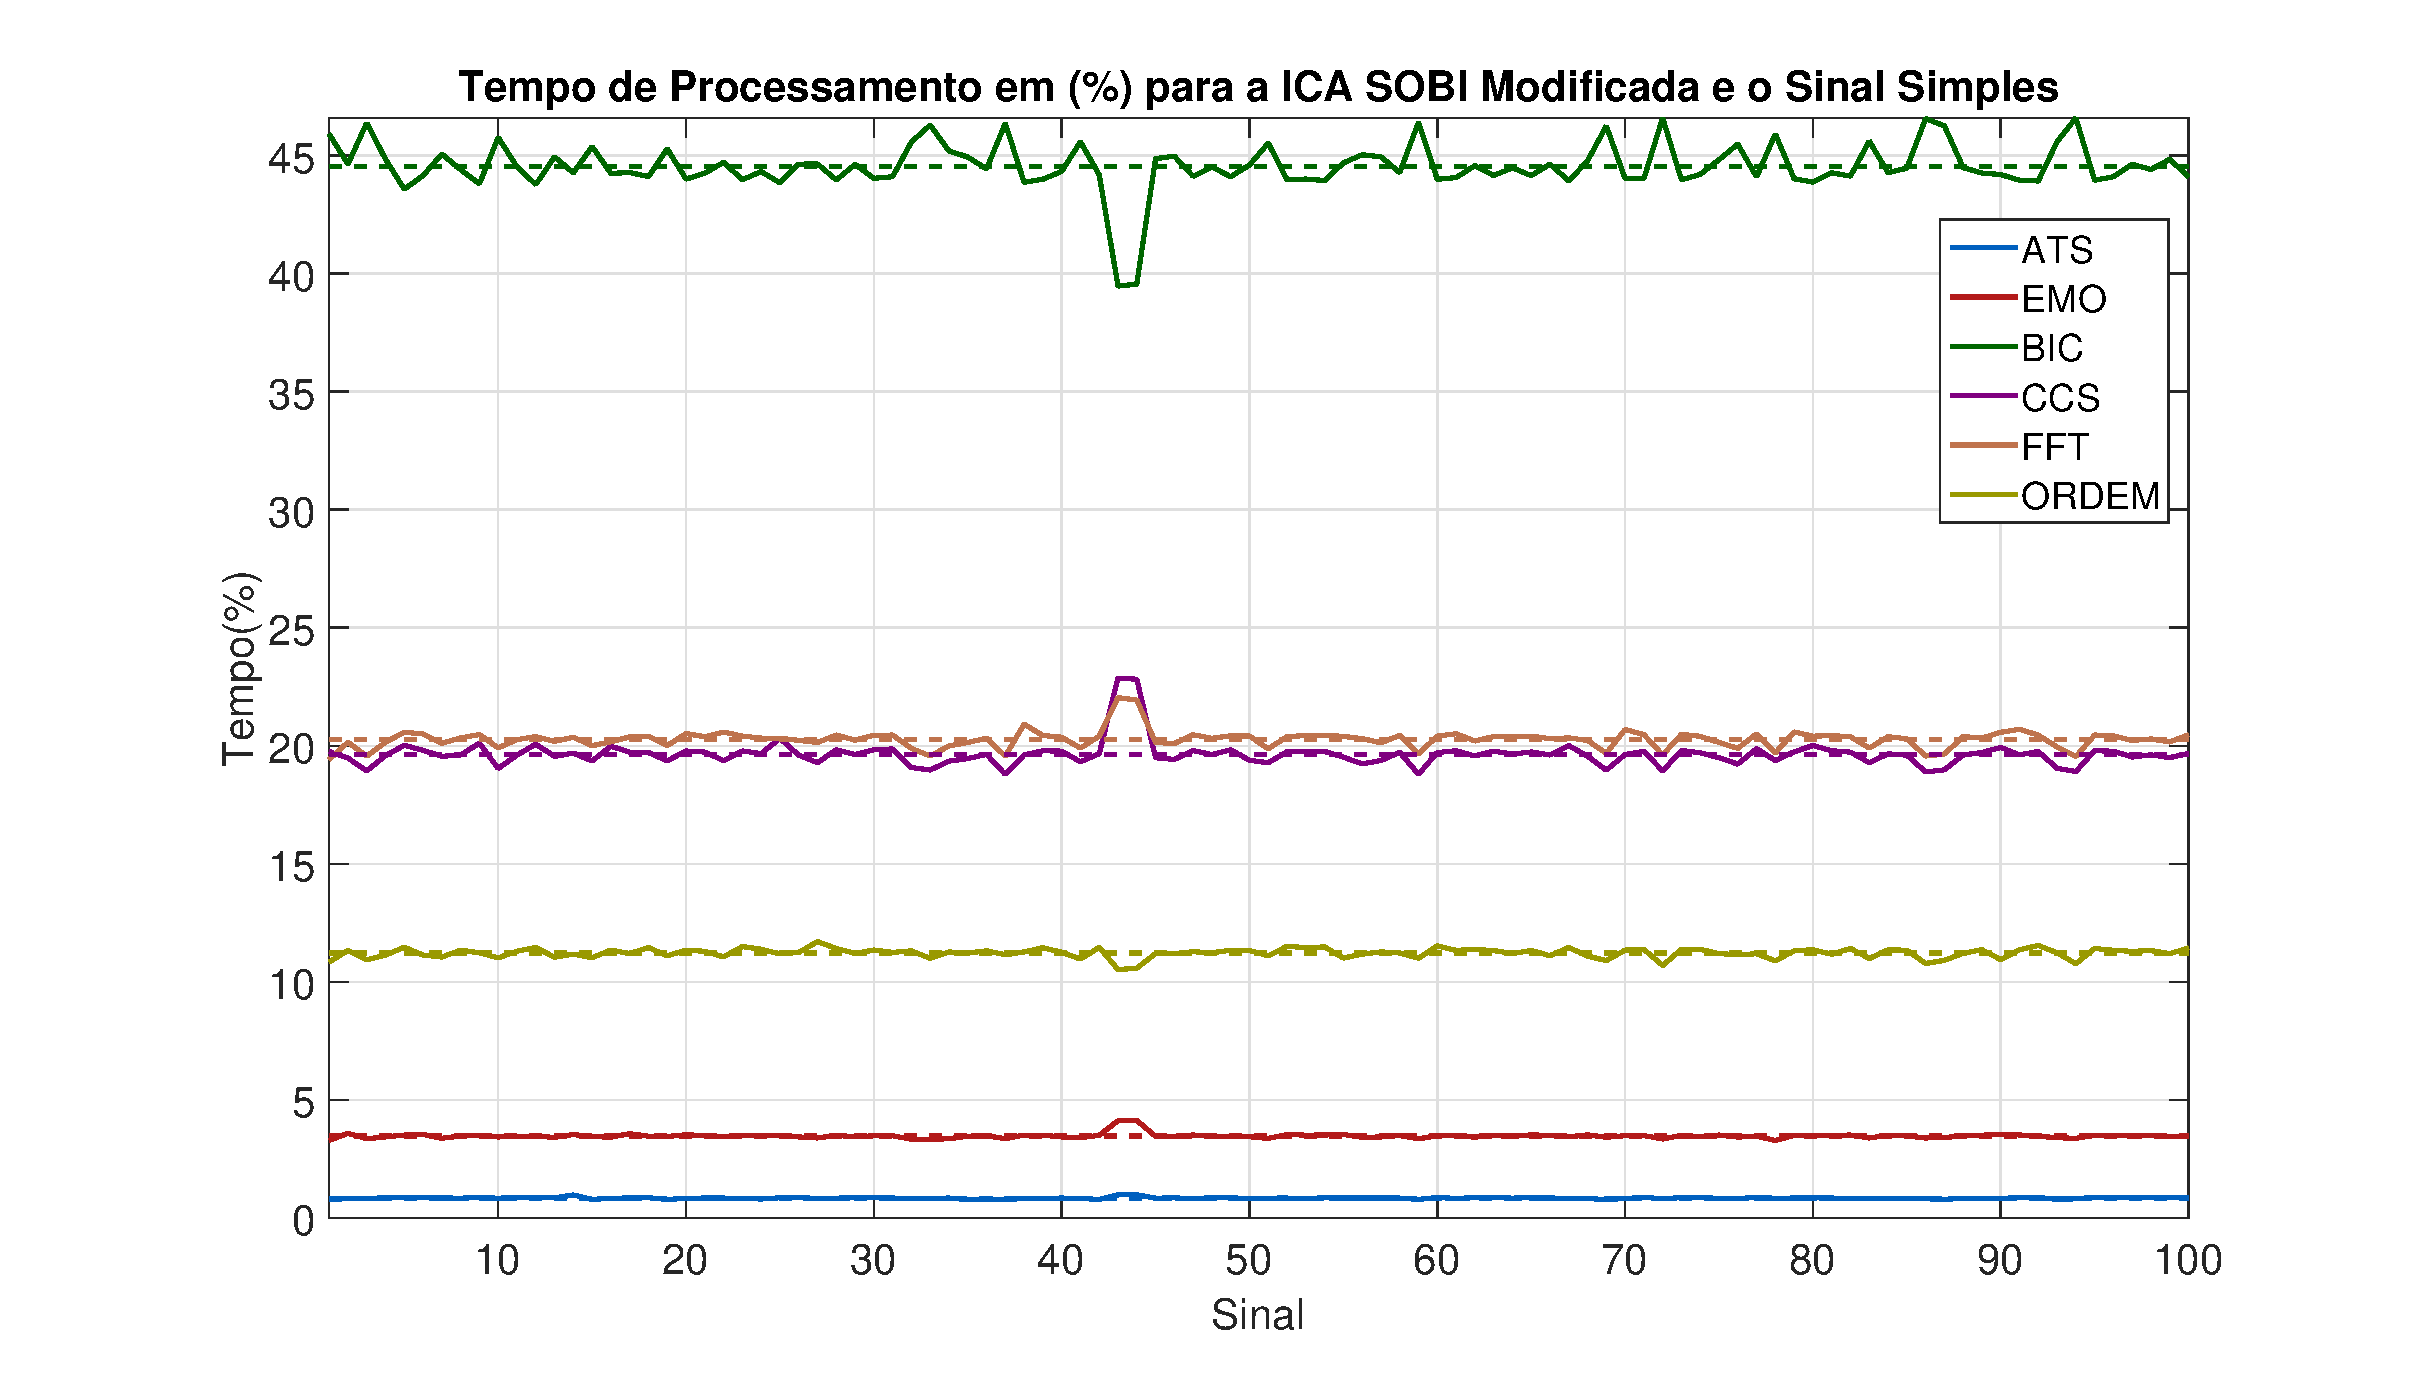
\includegraphics[scale=0.45]{imagens/ImagensParaOAnexo/TPPEICASOBImodSinalSimples.eps}
    \caption{TP em porcentagem de todos os testes para ICA SOBI modificada e um sinal com quatro componentes.}
    \label{fig:TPSMSinalsimples}    
    \end{center}
\end{figure}

\begin{figure}[!htb]
    \begin{center}
    \advance\leftskip -1.5cm
    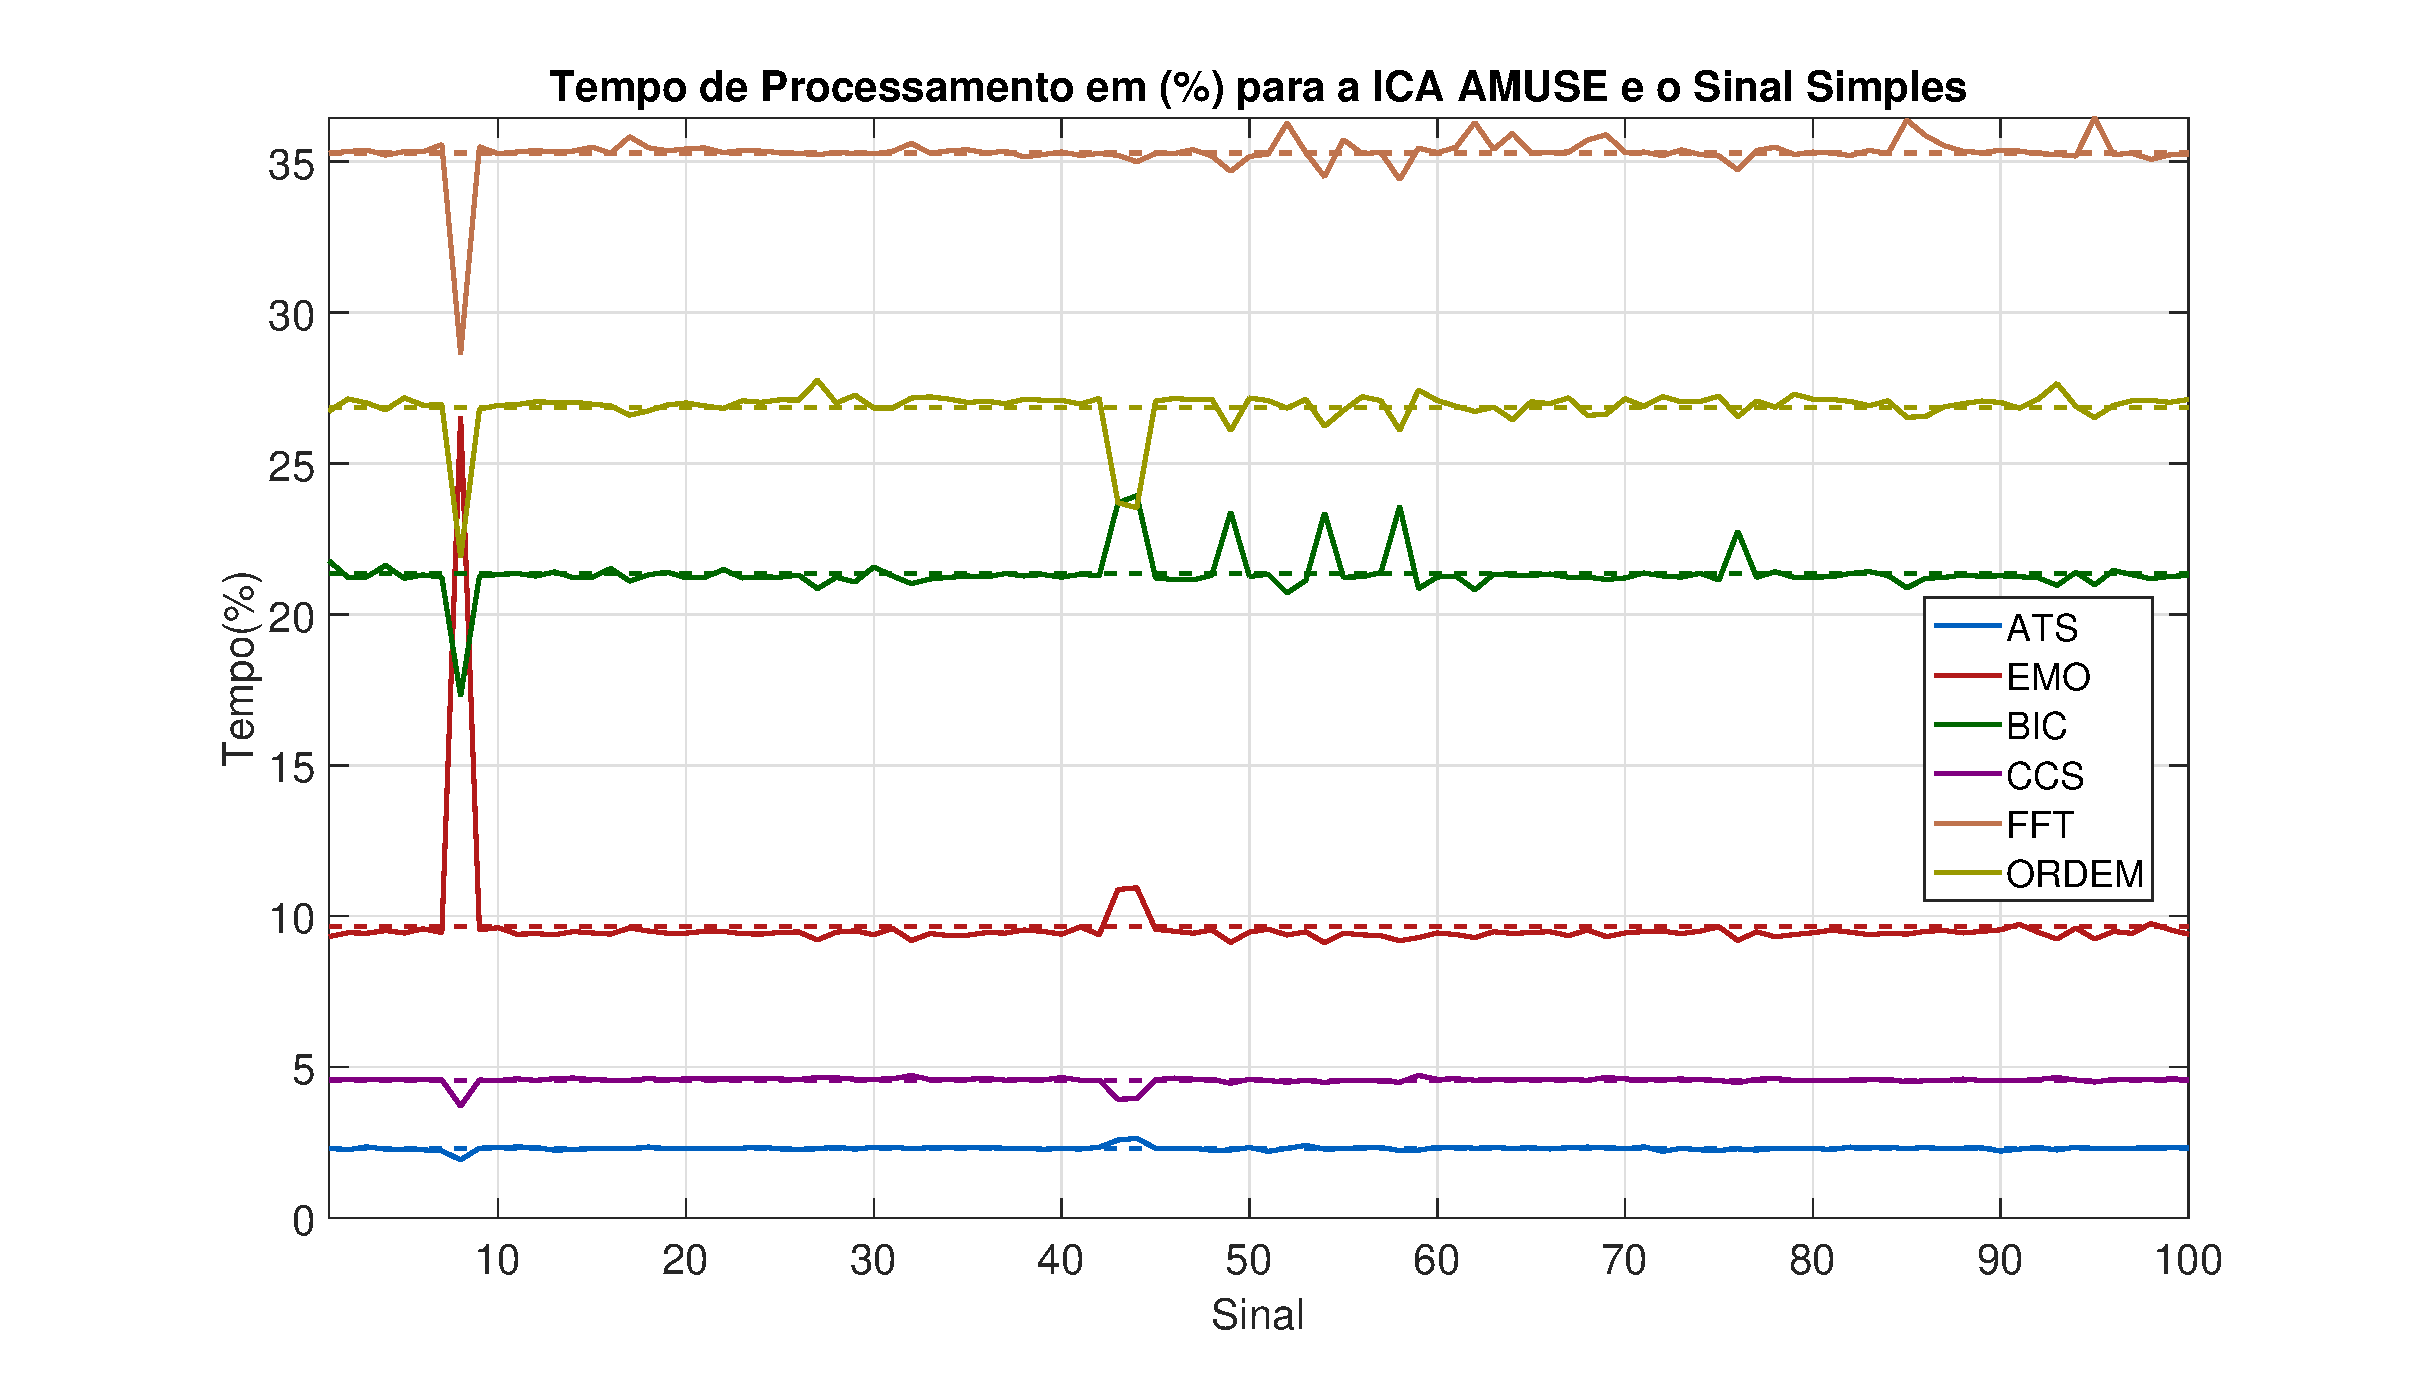
\includegraphics[scale=0.45]{imagens/ImagensParaOAnexo/TPPEICAAMUSeSinalSimples.eps}
    \caption{TP em porcentagem de todos os testes para ICA AMUSE e um sinal com quatro componentes.}
    \label{fig:TPAMSinalsimples}    
    \end{center}
\end{figure}

\begin{figure}[!htb]
    \begin{center}
    \advance\leftskip -1.5cm
    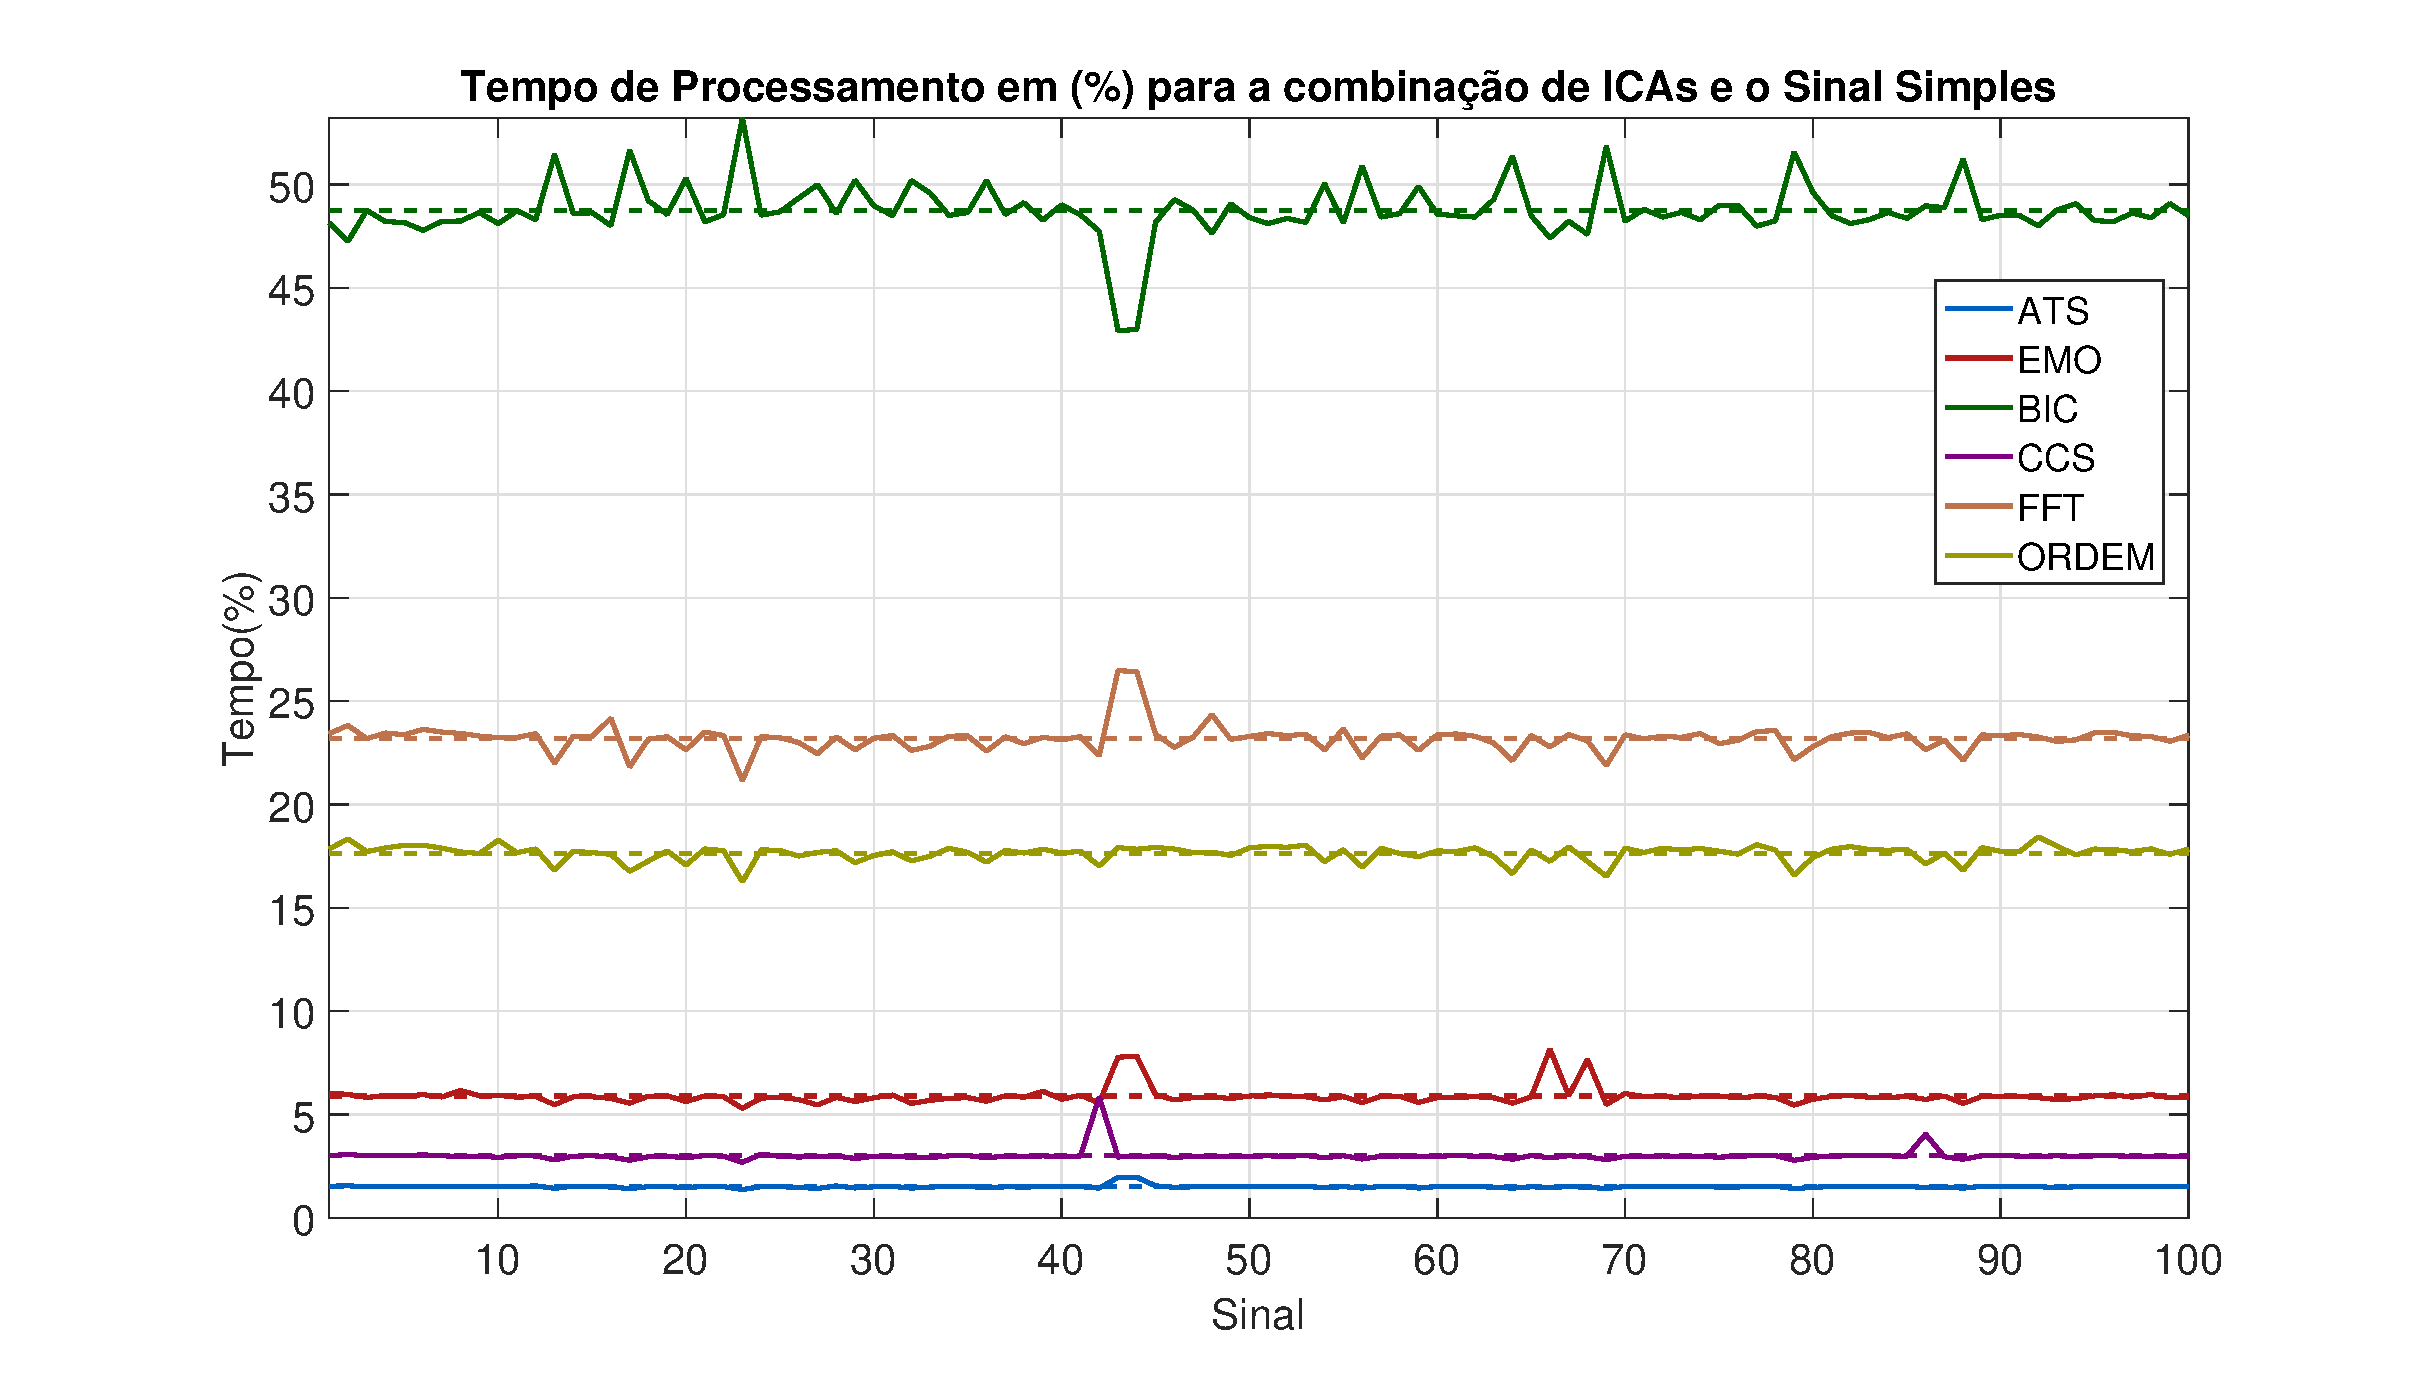
\includegraphics[scale=0.45]{imagens/ImagensParaOAnexo/TPPECombinacaoICASinalSimples.eps}
    \caption{TP em porcentagem de todos os testes para combinação de ICAs  e um sinal com quatro componentes.}
    \label{fig:TPCISinalsimples}    
    \end{center}
\end{figure}

\begin{figure}[!htb]
    \begin{center}
    \advance\leftskip -1.5cm
    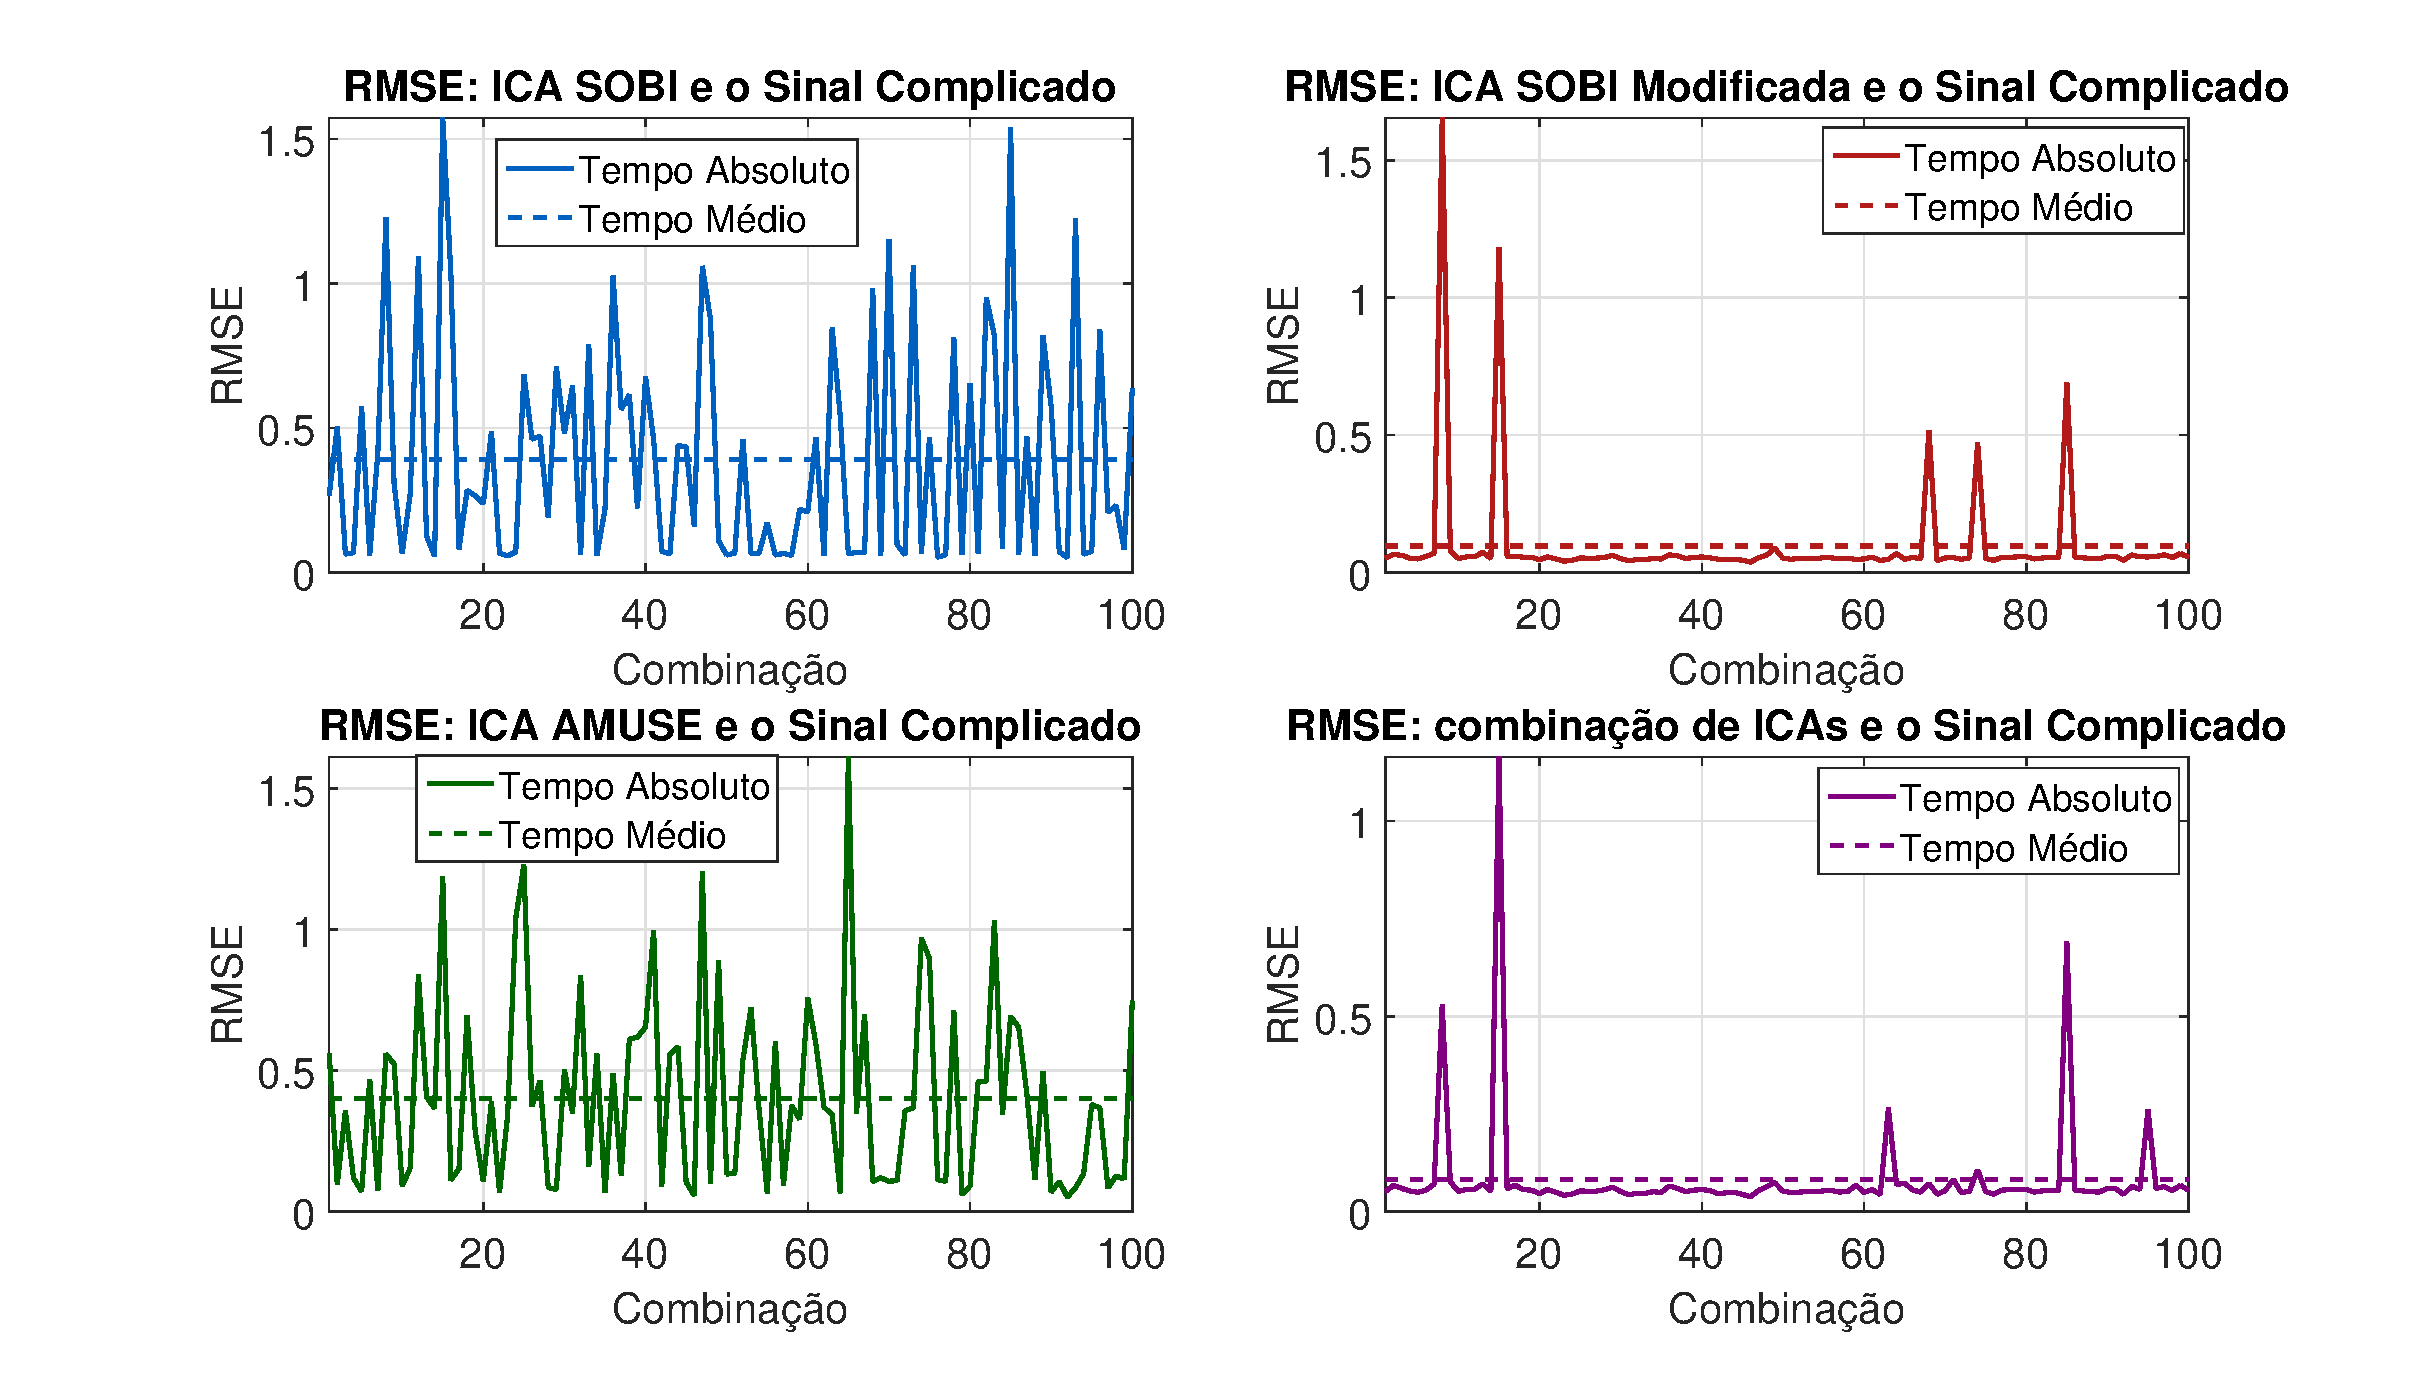
\includegraphics[scale=0.45]{imagens/ImagensParaOAnexo/RMSEETodasICAsSinalComplicado.eps}
    \caption{RMSE de todos os testes e todas as ICAs para um sinal complicado.}
    \label{fig:RMSESinalComplicado}    
    \end{center}
\end{figure}

\begin{figure}[!htb]
    \begin{center}
    \advance\leftskip -1.5cm
    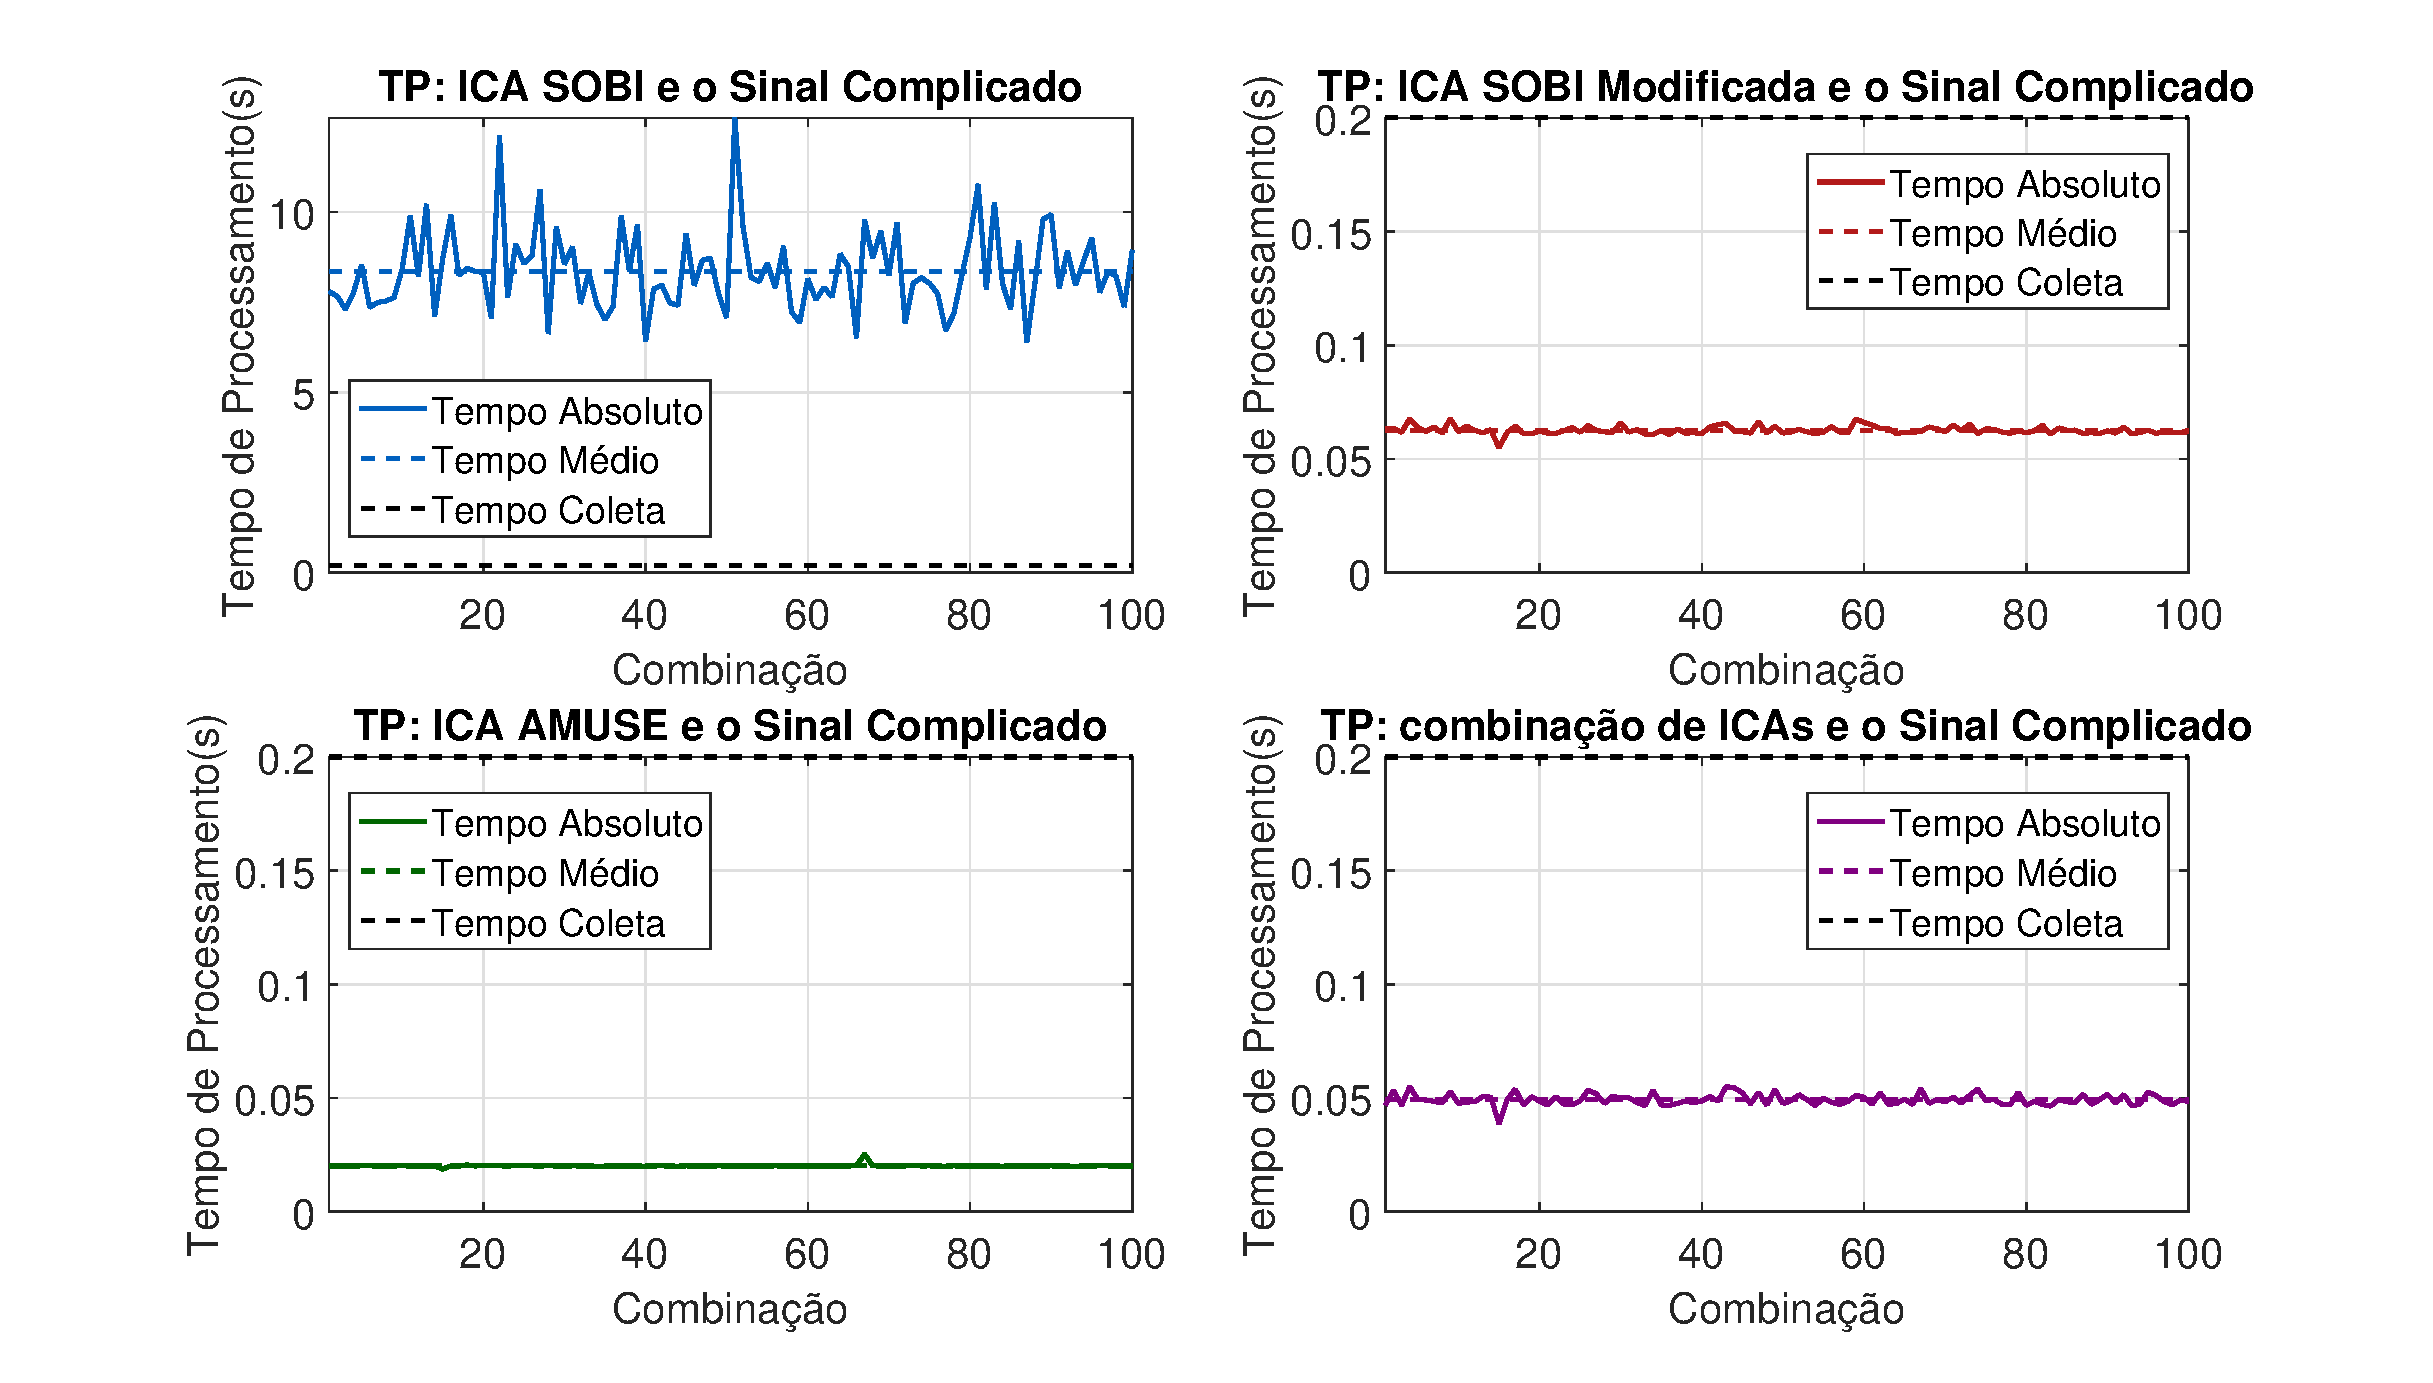
\includegraphics[scale=0.45]{imagens/ImagensParaOAnexo/TPAETodasICAsSinalComplicado.eps}
    \caption{TP de todos os testes e todas as ICAs para um sinal complicado.}
    \label{fig:TPSinalComplicado}    
    \end{center}
\end{figure}

\begin{figure}[!htb]
    \begin{center}
    \advance\leftskip -1.5cm
    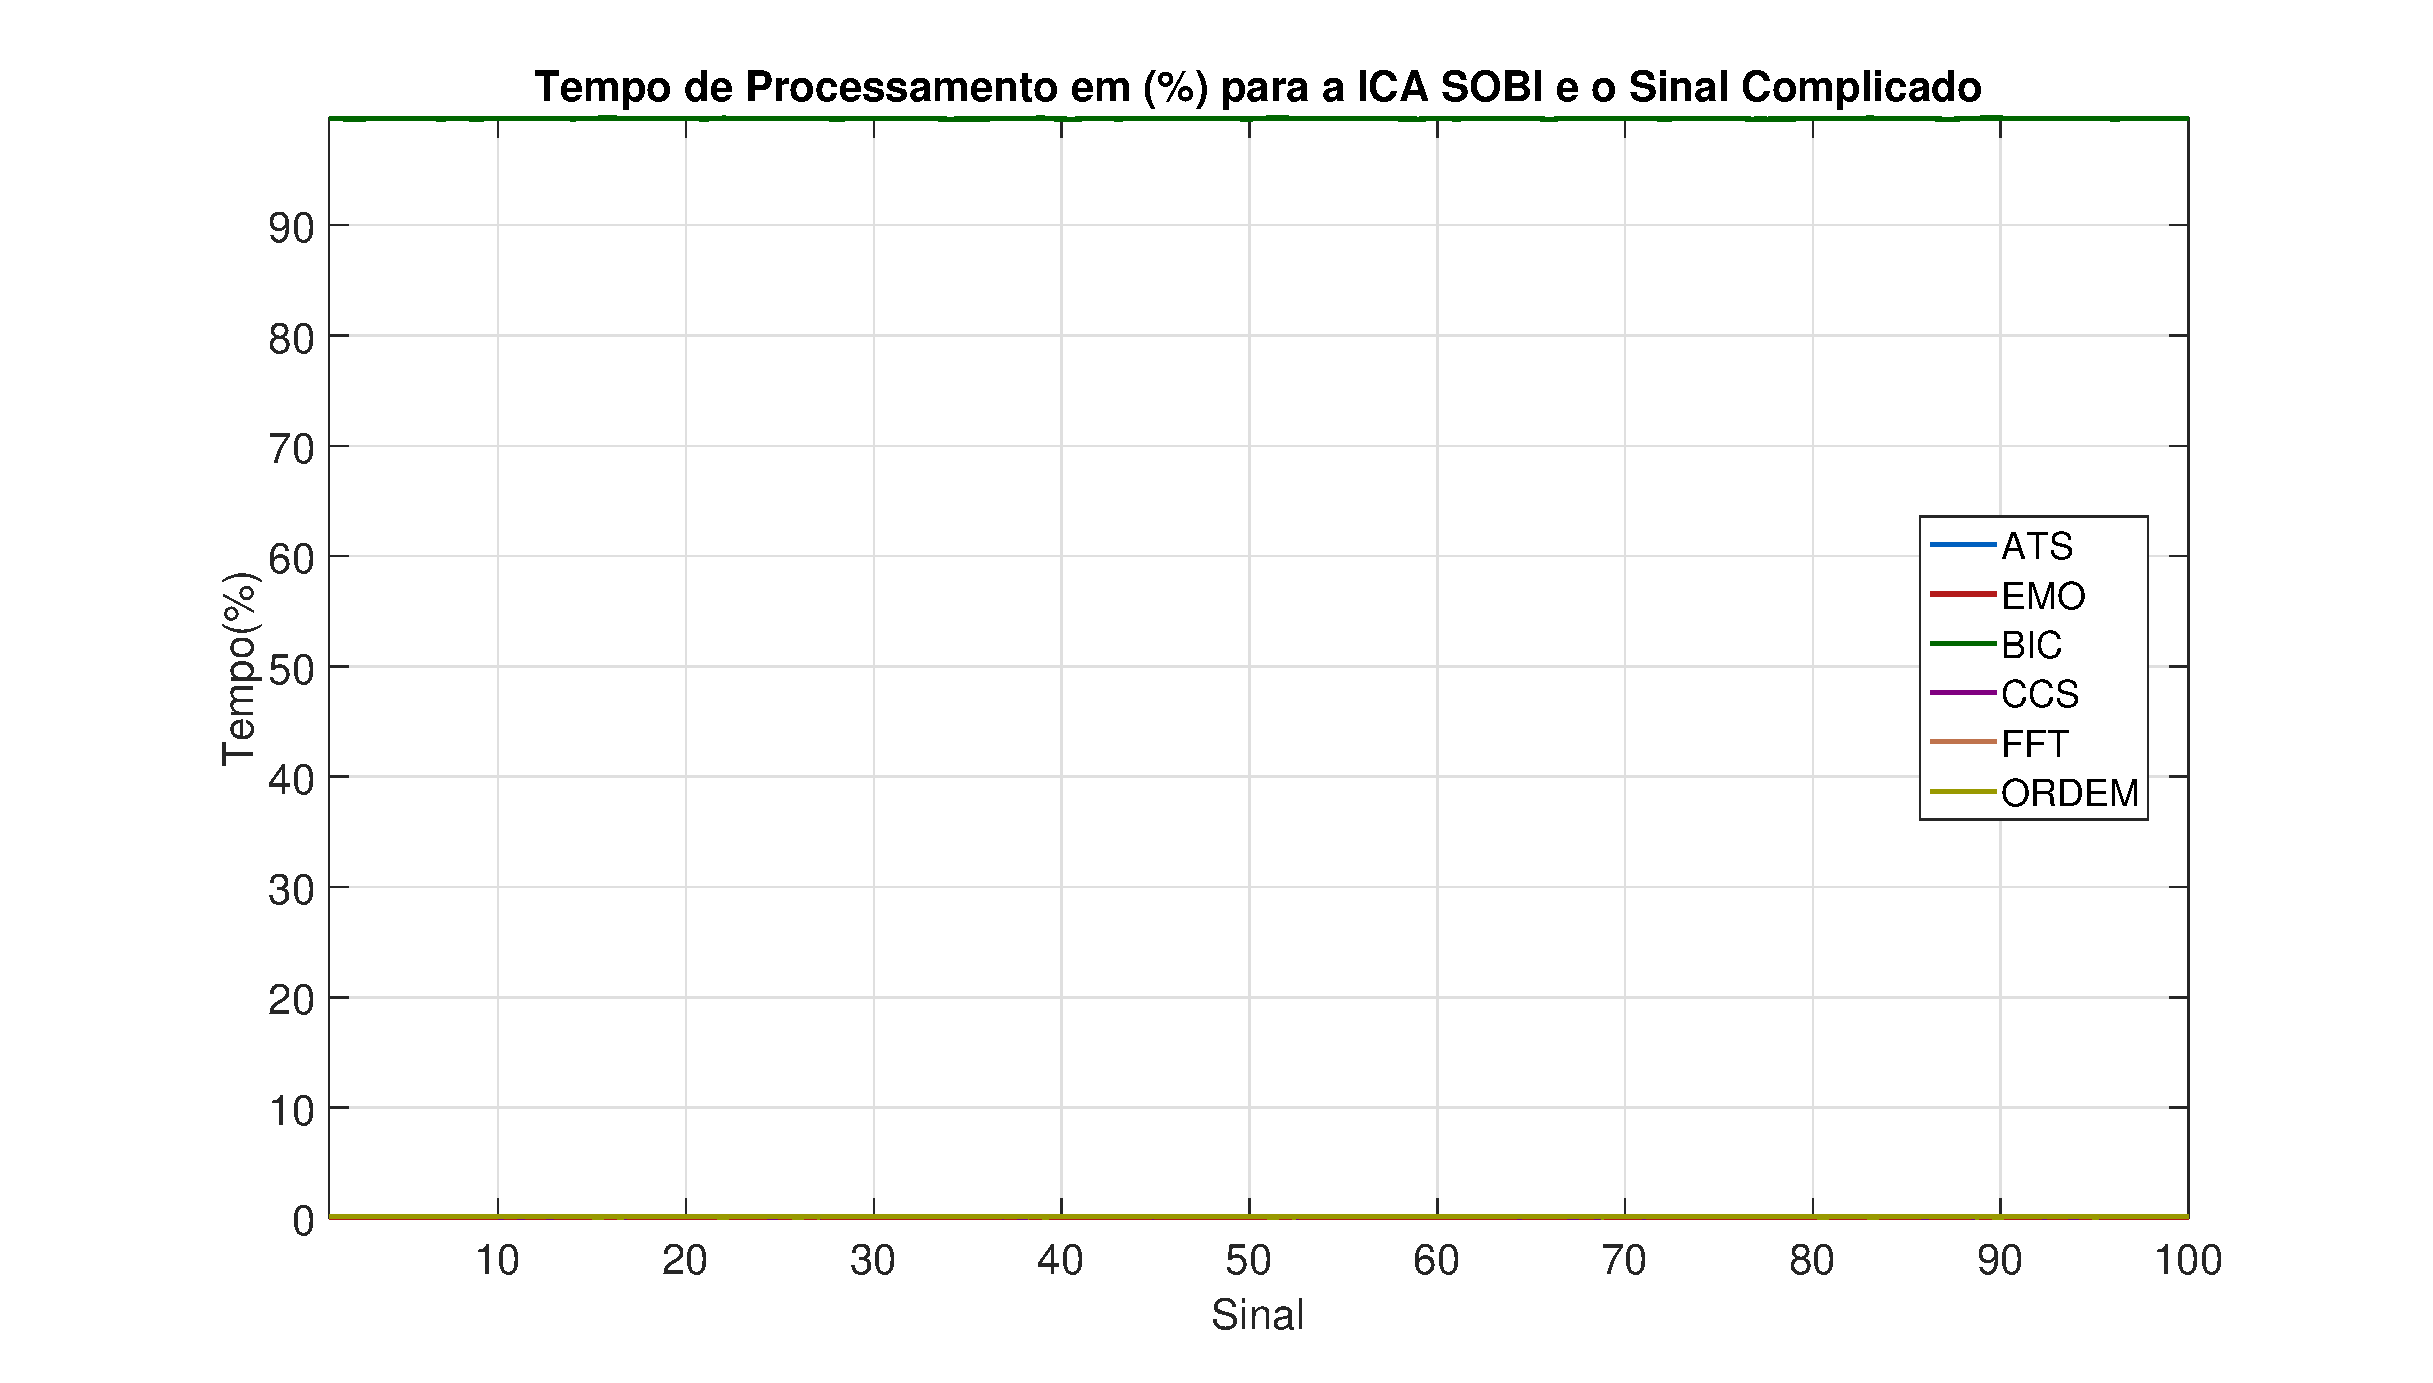
\includegraphics[scale=0.45]{imagens/ImagensParaOAnexo/TPPEICASOBISinalComplicado.eps}
    \caption{TP em porcentagem de todos os testes para ICA SOBI e um sinal complicado.}
    \label{fig:TPSSSinalComplicado}    
    \end{center}
\end{figure}

\begin{figure}[!htb]
    \begin{center}
    \advance\leftskip -1.5cm
    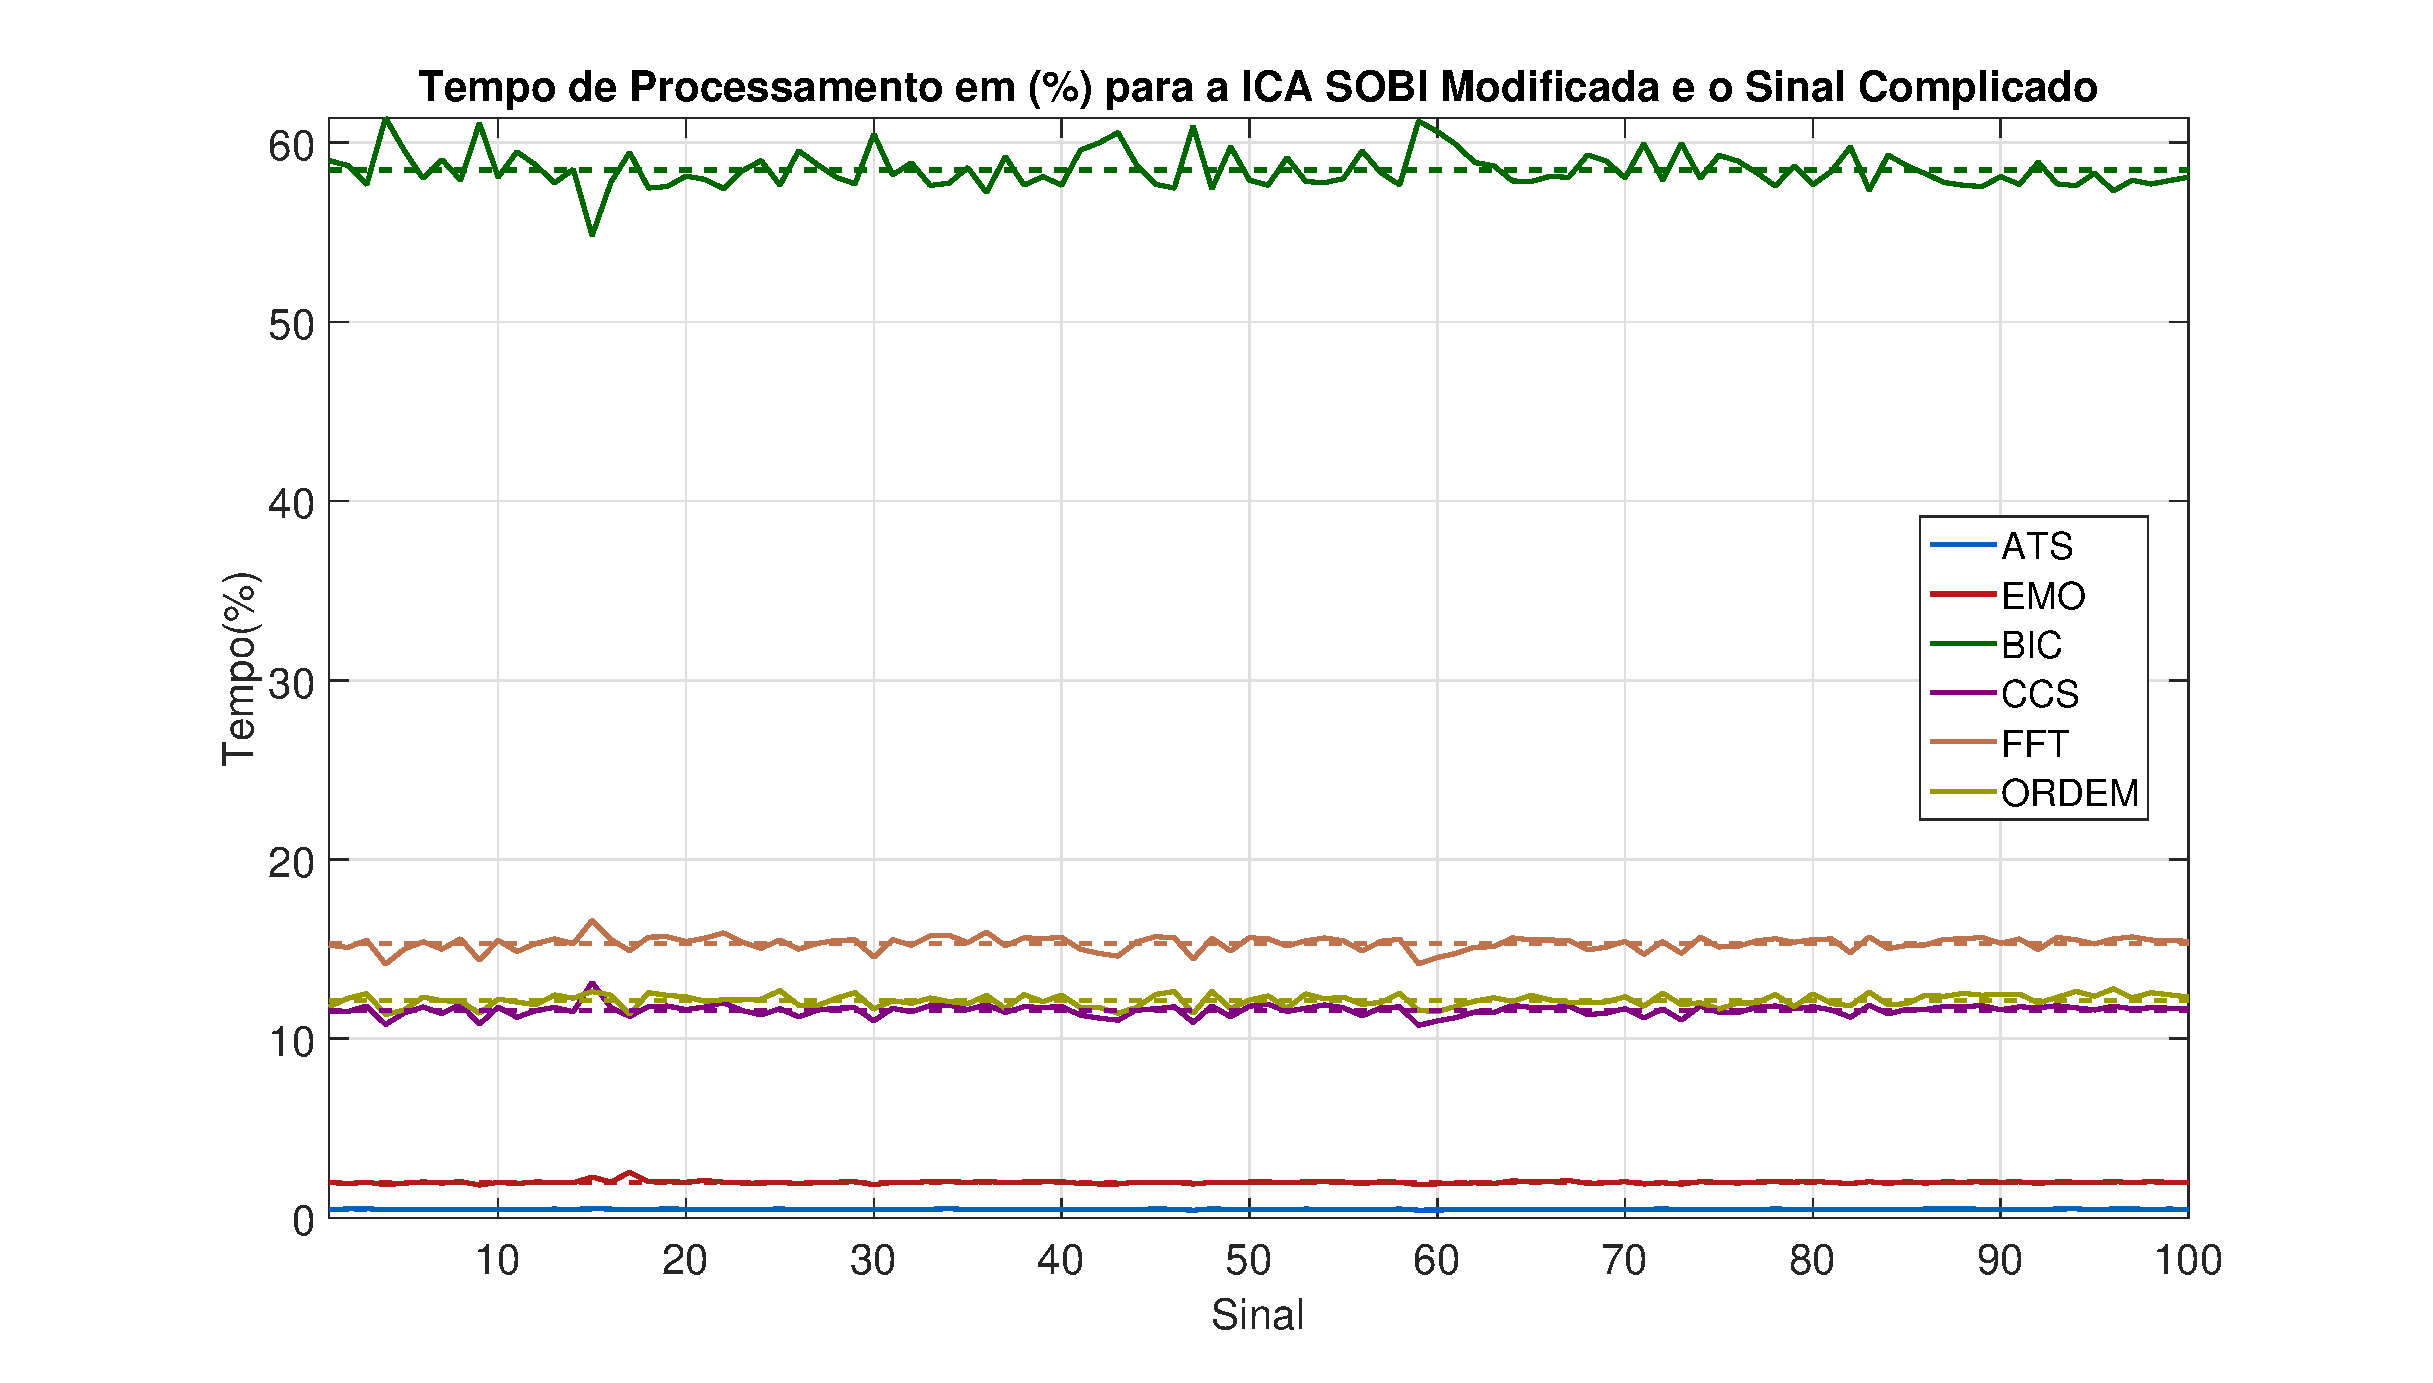
\includegraphics[scale=0.45]{imagens/ImagensParaOAnexo/TPPEICASOBImodSinalComplicado.eps}
    \caption{TP em porcentagem de todos os testes para ICA SOBI modificada e um sinal complicado.}
    \label{fig:TPSMSinalComplicado}    
    \end{center}
\end{figure}

\begin{figure}[!htb]
    \begin{center}
    \advance\leftskip -1.5cm
    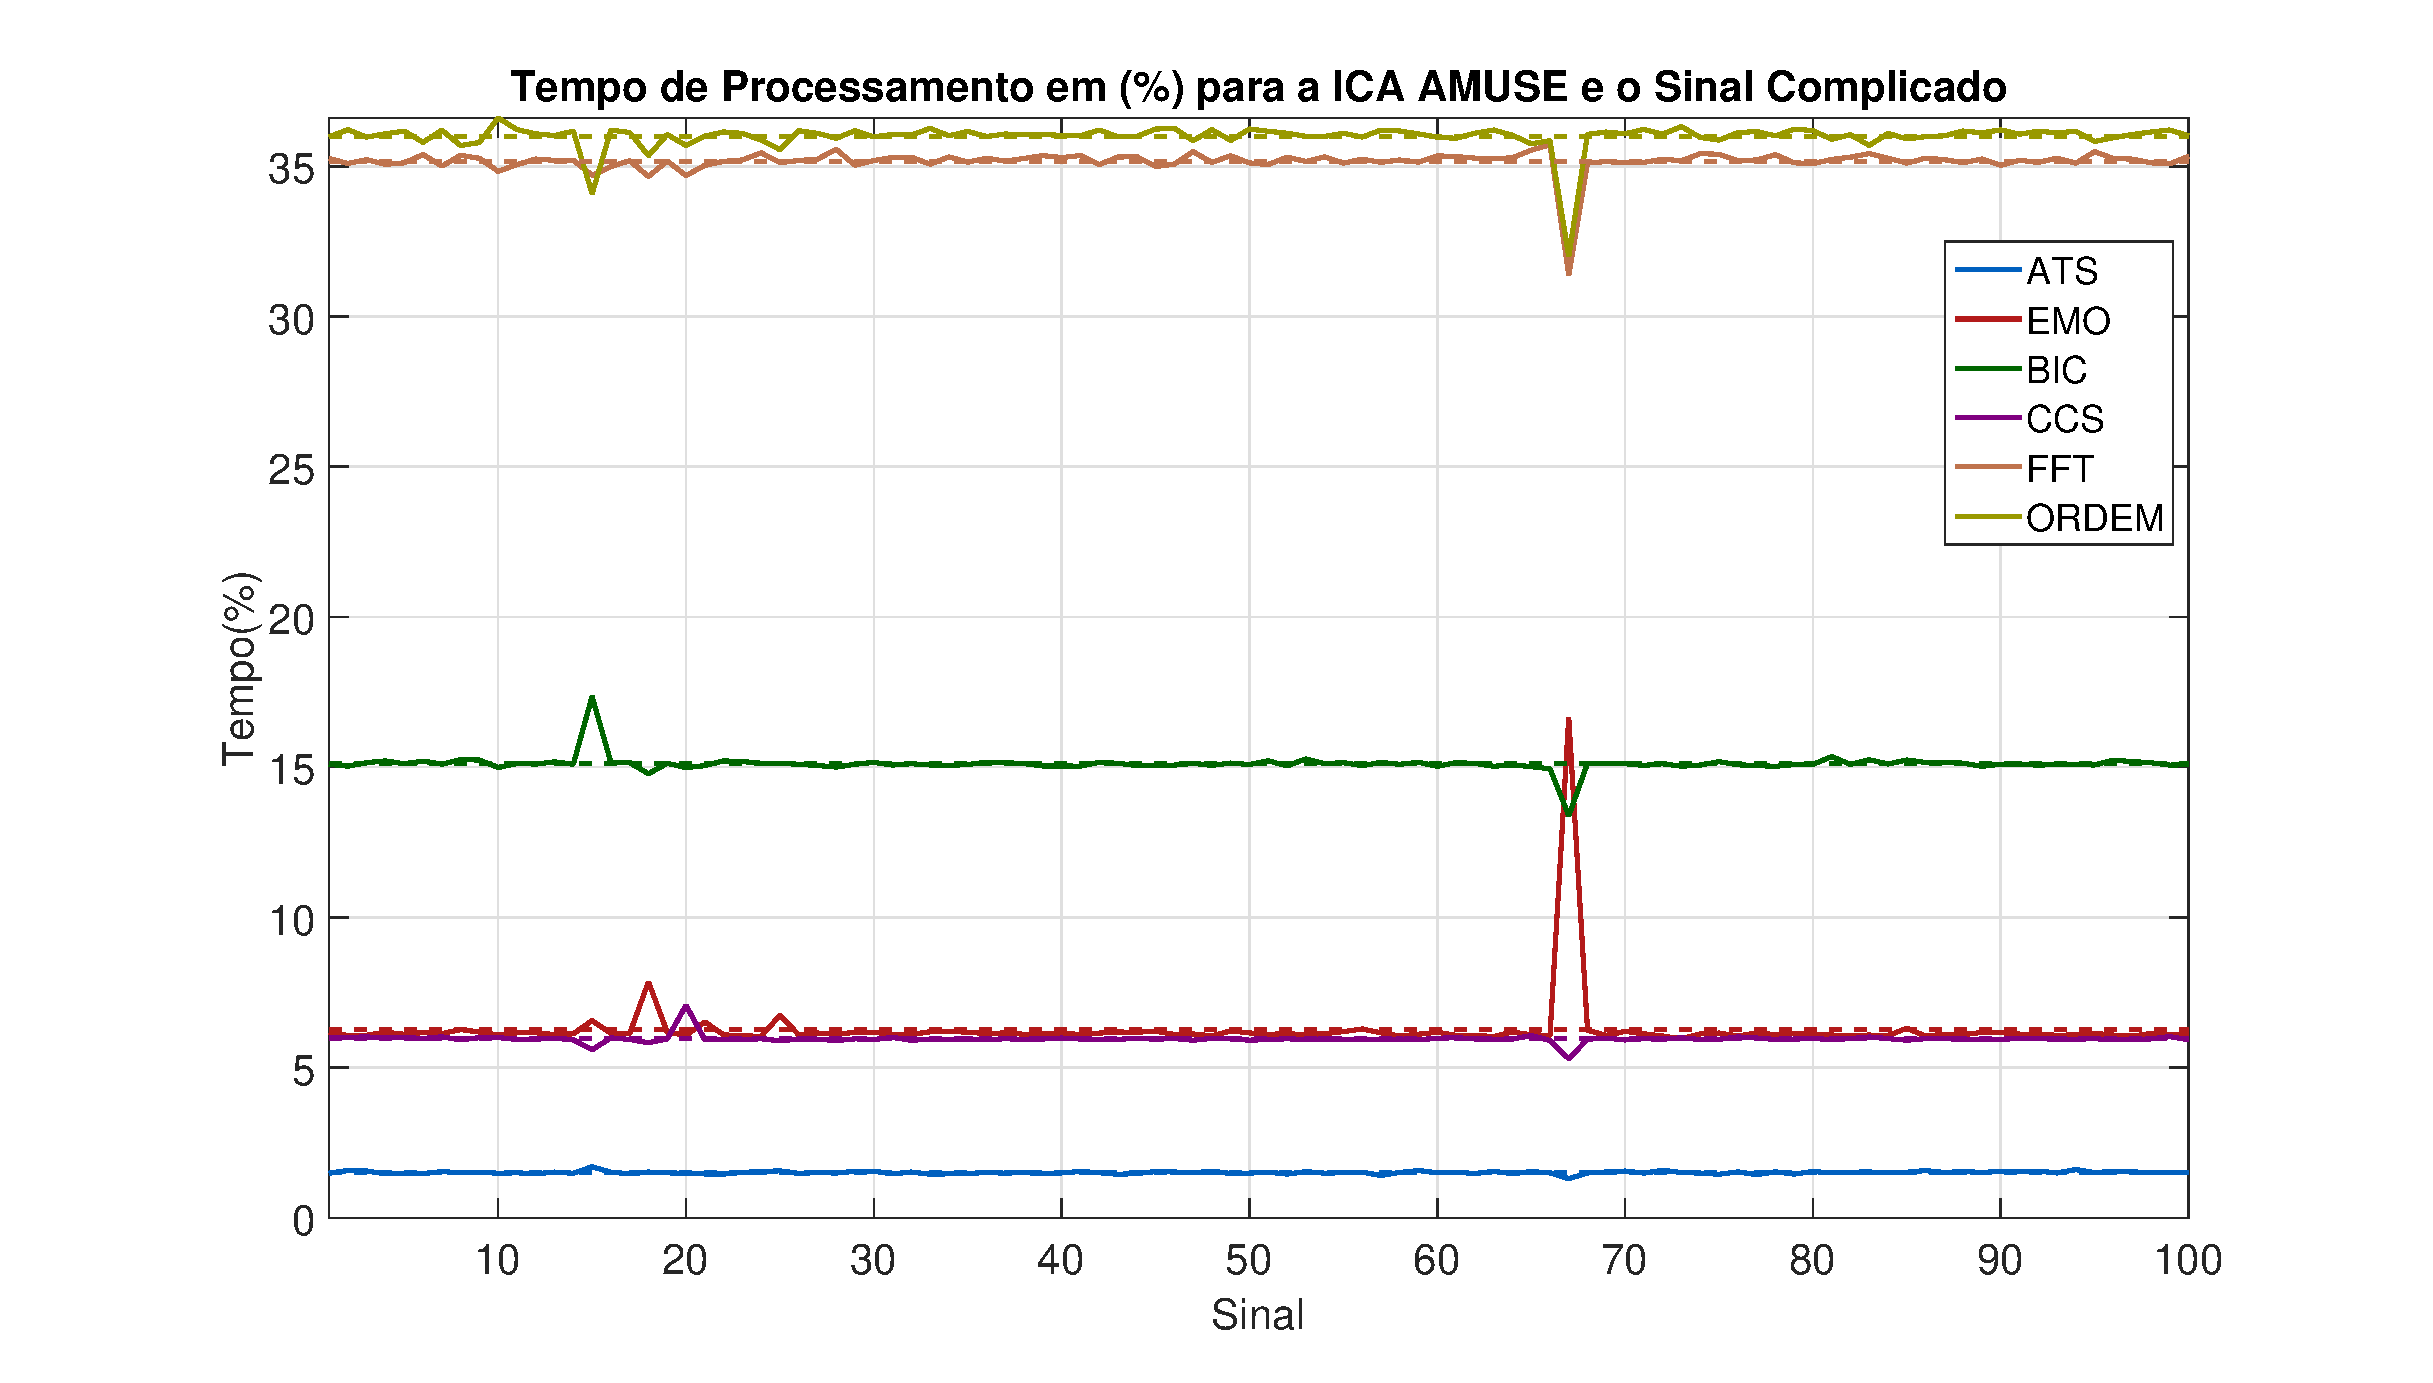
\includegraphics[scale=0.45]{imagens/ImagensParaOAnexo/TPPEICAAMUSeSinalComplicado.eps}
    \caption{TP em porcentagem de todos os testes para ICA AMUSE e um sinal complicado.}
    \label{fig:TPAMSinalComplicado}    
    \end{center}
\end{figure}

\begin{figure}[!htb]
    \begin{center}
    \advance\leftskip -1.5cm
    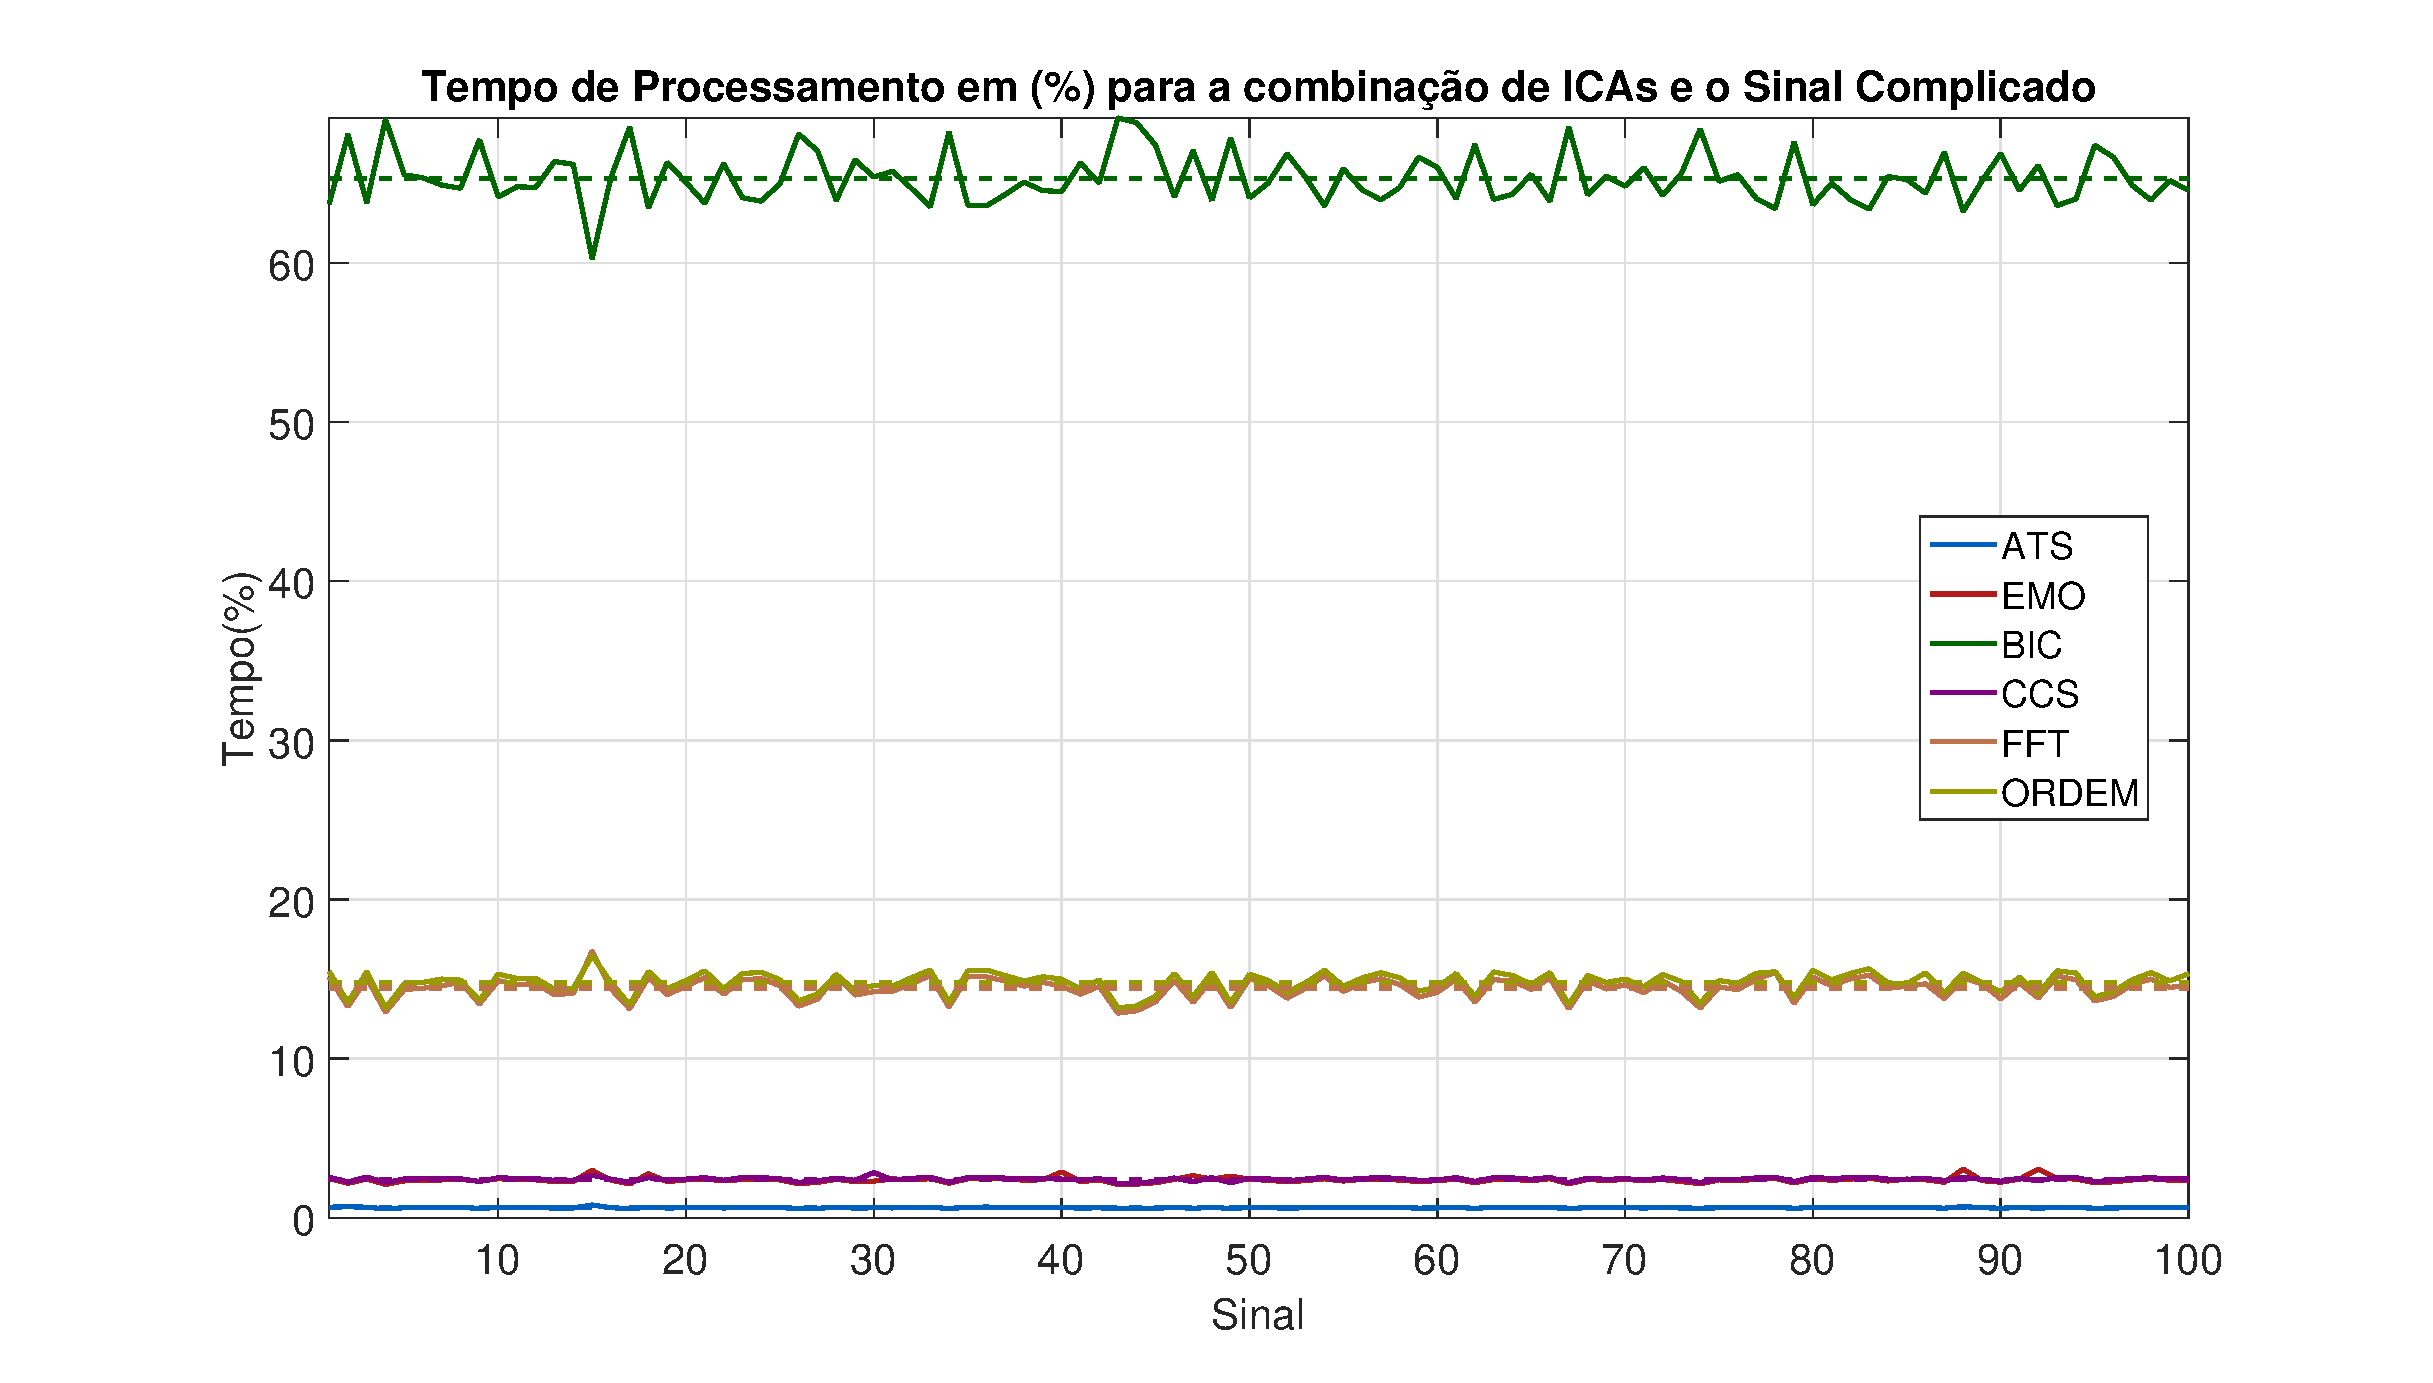
\includegraphics[scale=0.45]{imagens/ImagensParaOAnexo/TPPECombinacaoICASinalComplicado.eps}
    \caption{TP em porcentagem de todos os testes para combinação de ICAs  e um sinal complicado.}
    \label{fig:TPCISinalComplicado}    
    \end{center}
\end{figure}

\begin{figure}[!htb]
    \begin{center}
    \advance\leftskip -1.5cm
    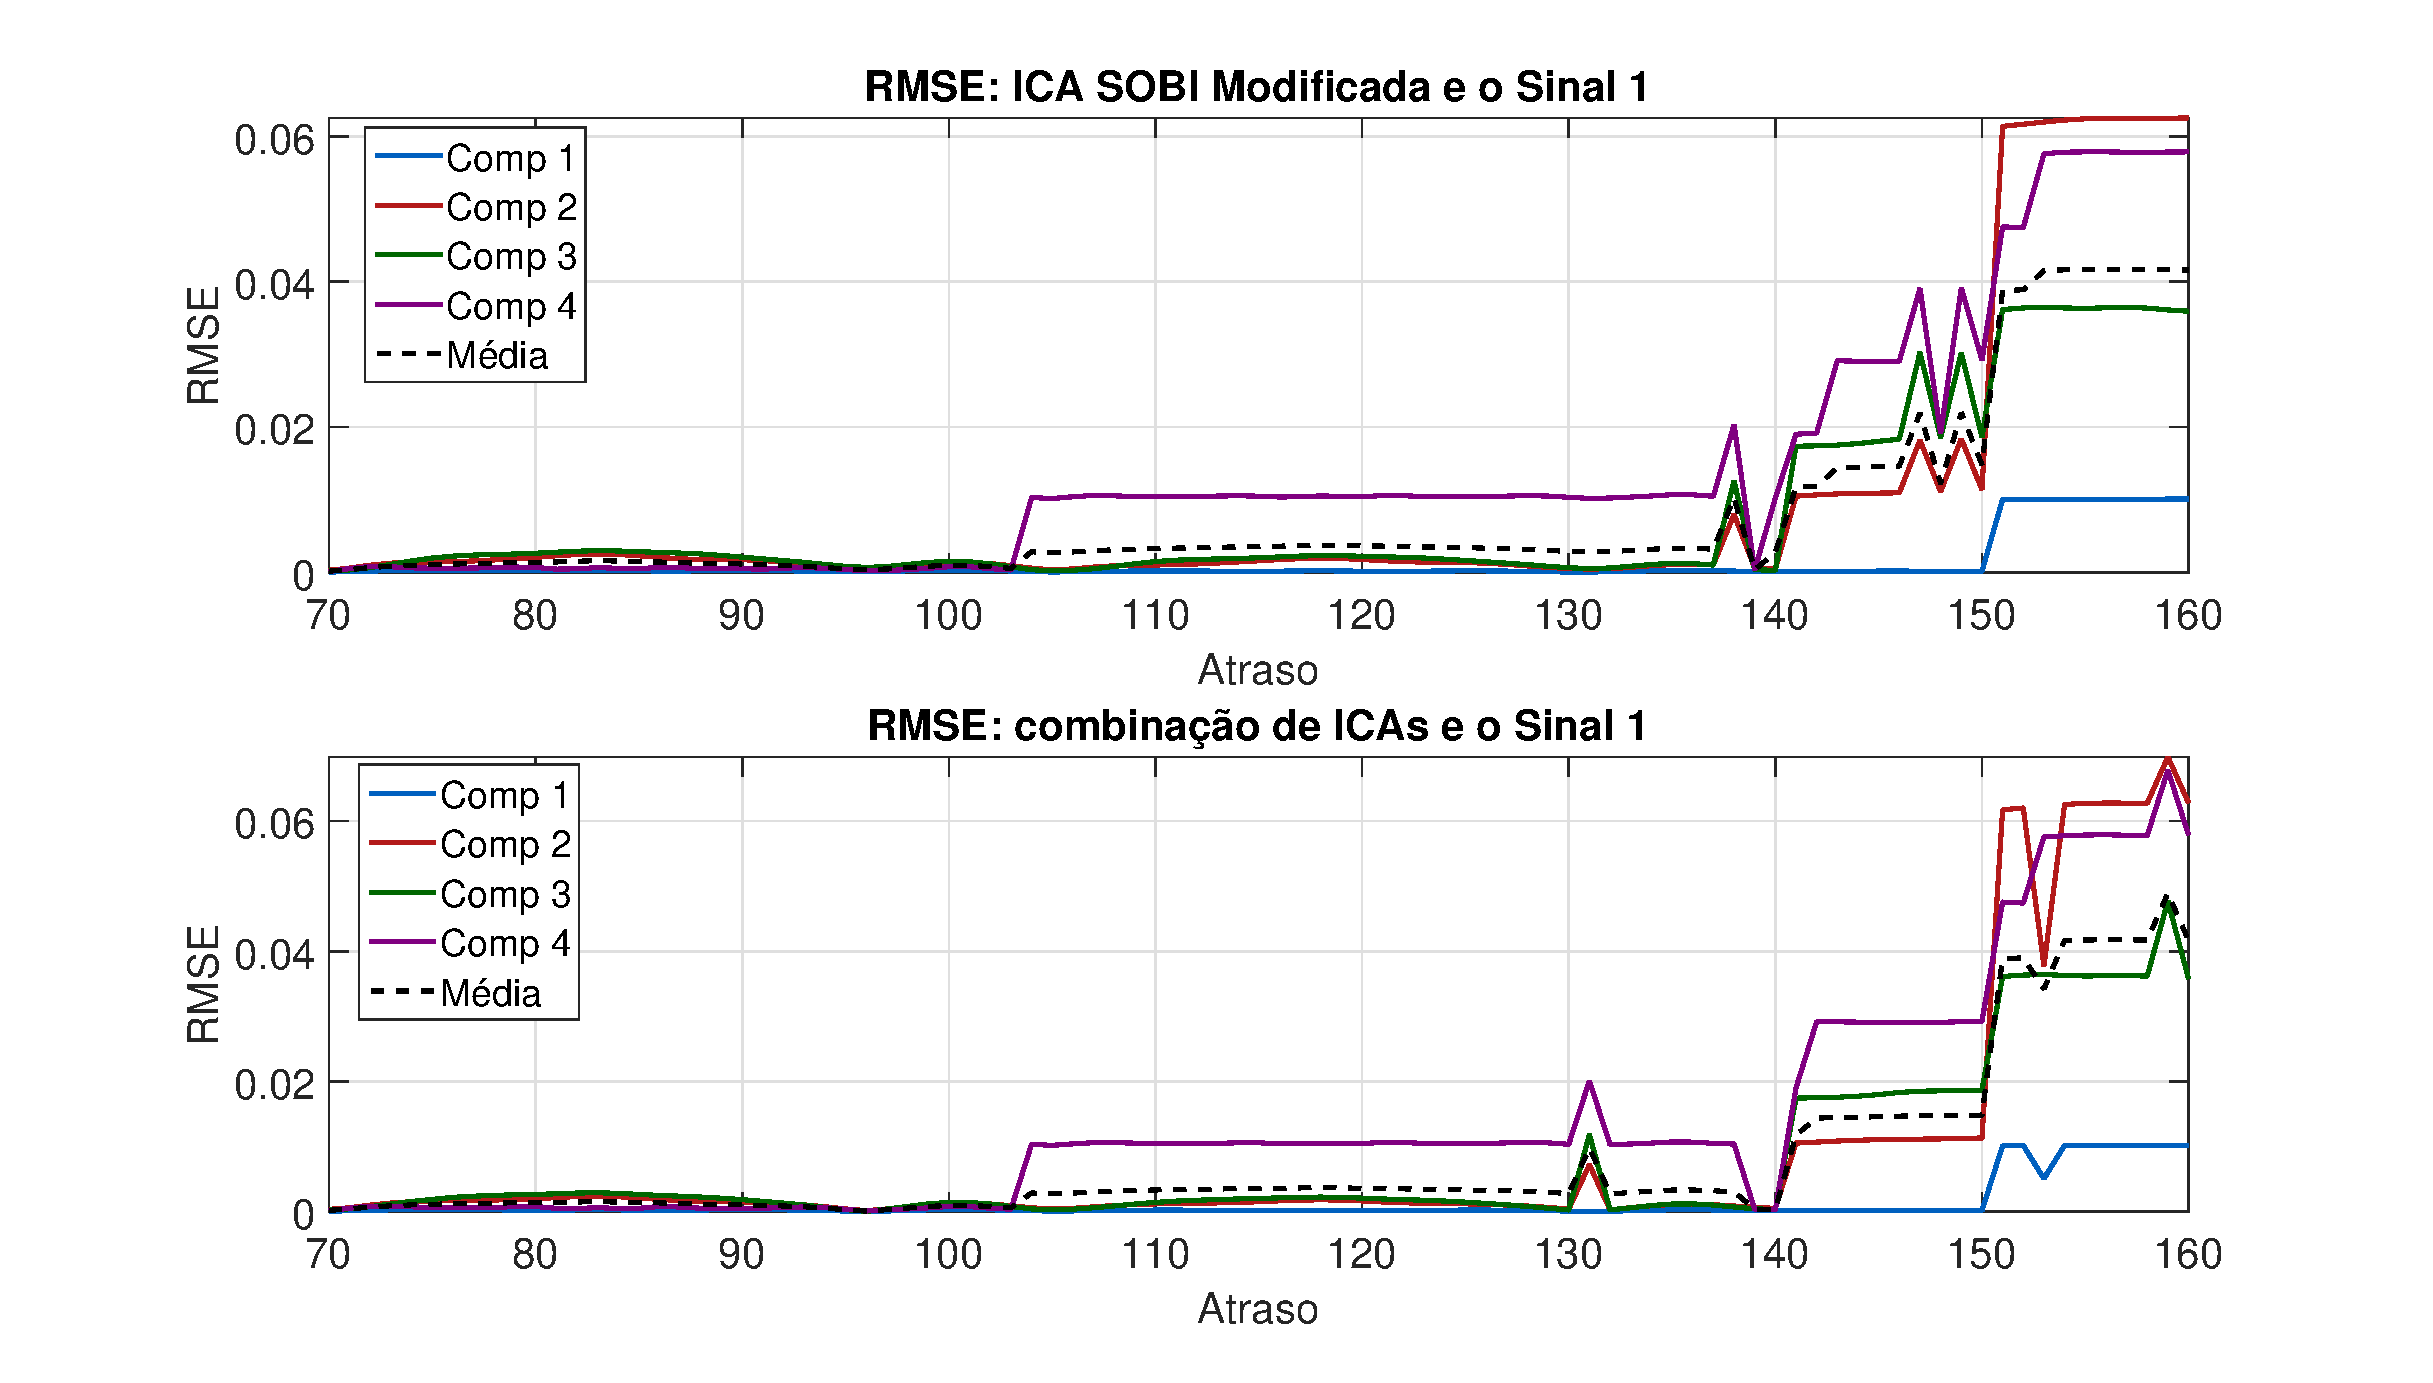
\includegraphics[scale=0.45]{imagens/ImagensParaOAnexo/RMSEcompATodasICAsSinal1.eps}
    \caption{RMSE por componente para as ICAs utilizadas e o S1.}
    \label{fig:RMSEAS1}    
    \end{center}
\end{figure}

\begin{figure}[!htb]
    \begin{center}
    \advance\leftskip -1.5cm
    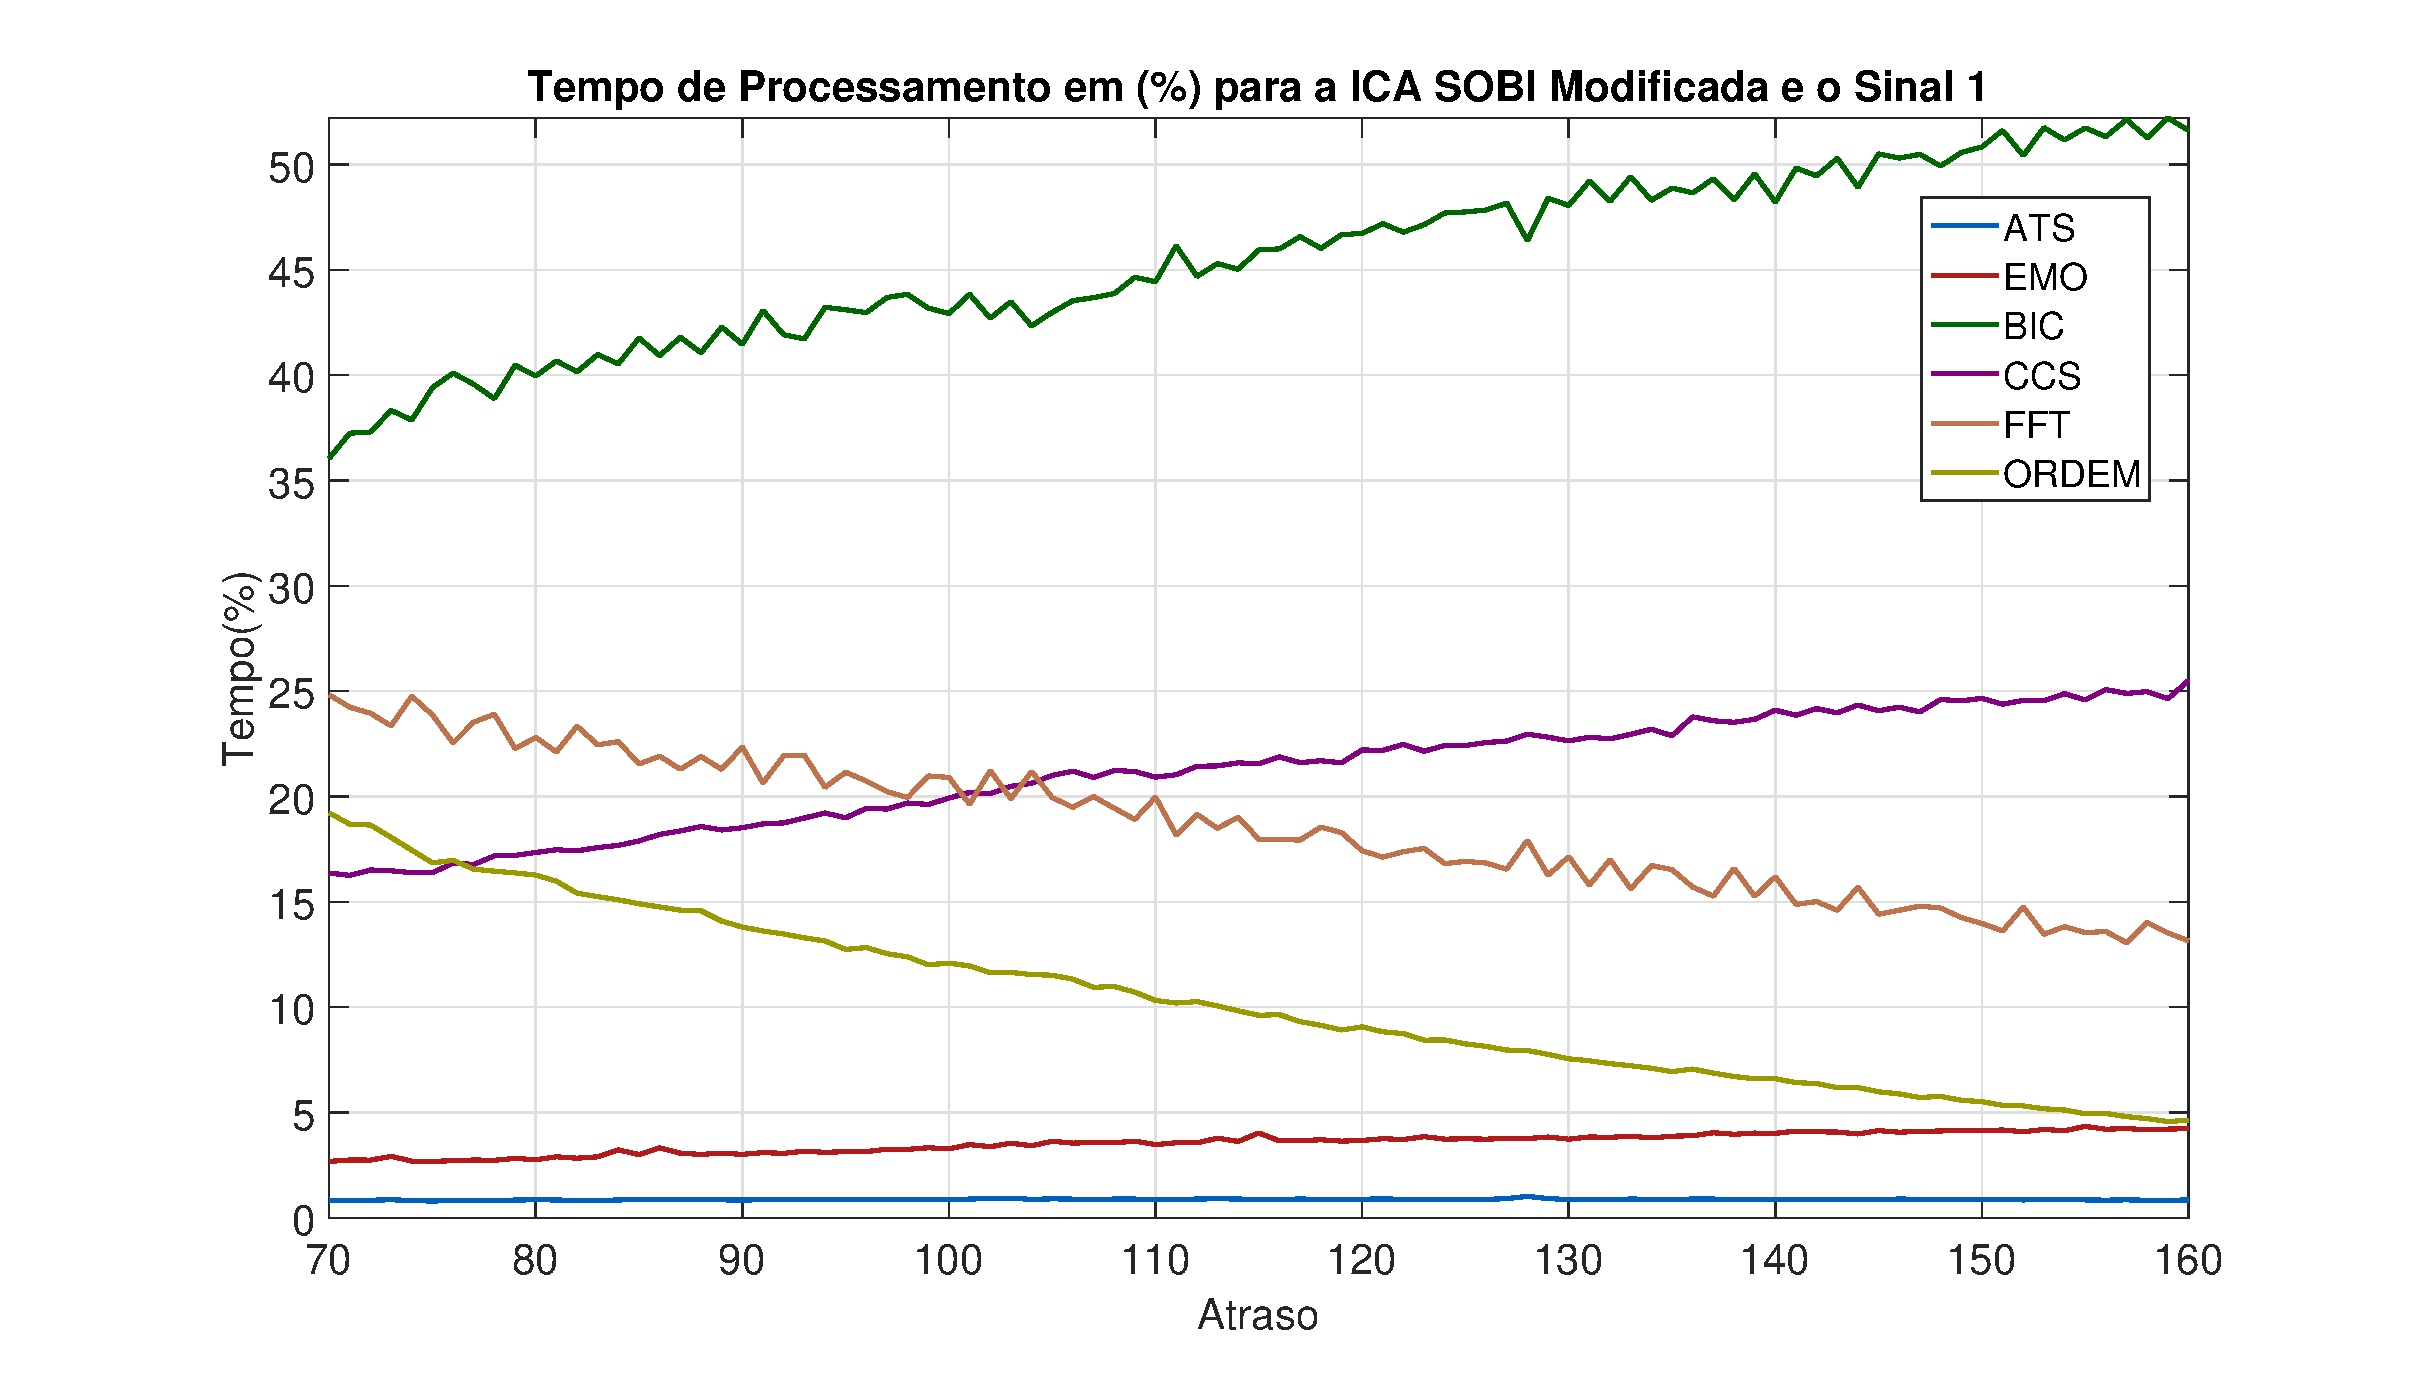
\includegraphics[scale=0.45]{imagens/ImagensParaOAnexo/TPPAICASOBImodSinal1.eps}
    \caption{TP em porcentagem dos testes para ICA SOBI modificado em S1.}
    \label{fig:TPSMAS1}    
    \end{center}
\end{figure}

\begin{figure}[!htb]
    \begin{center}
    \advance\leftskip -1.5cm
    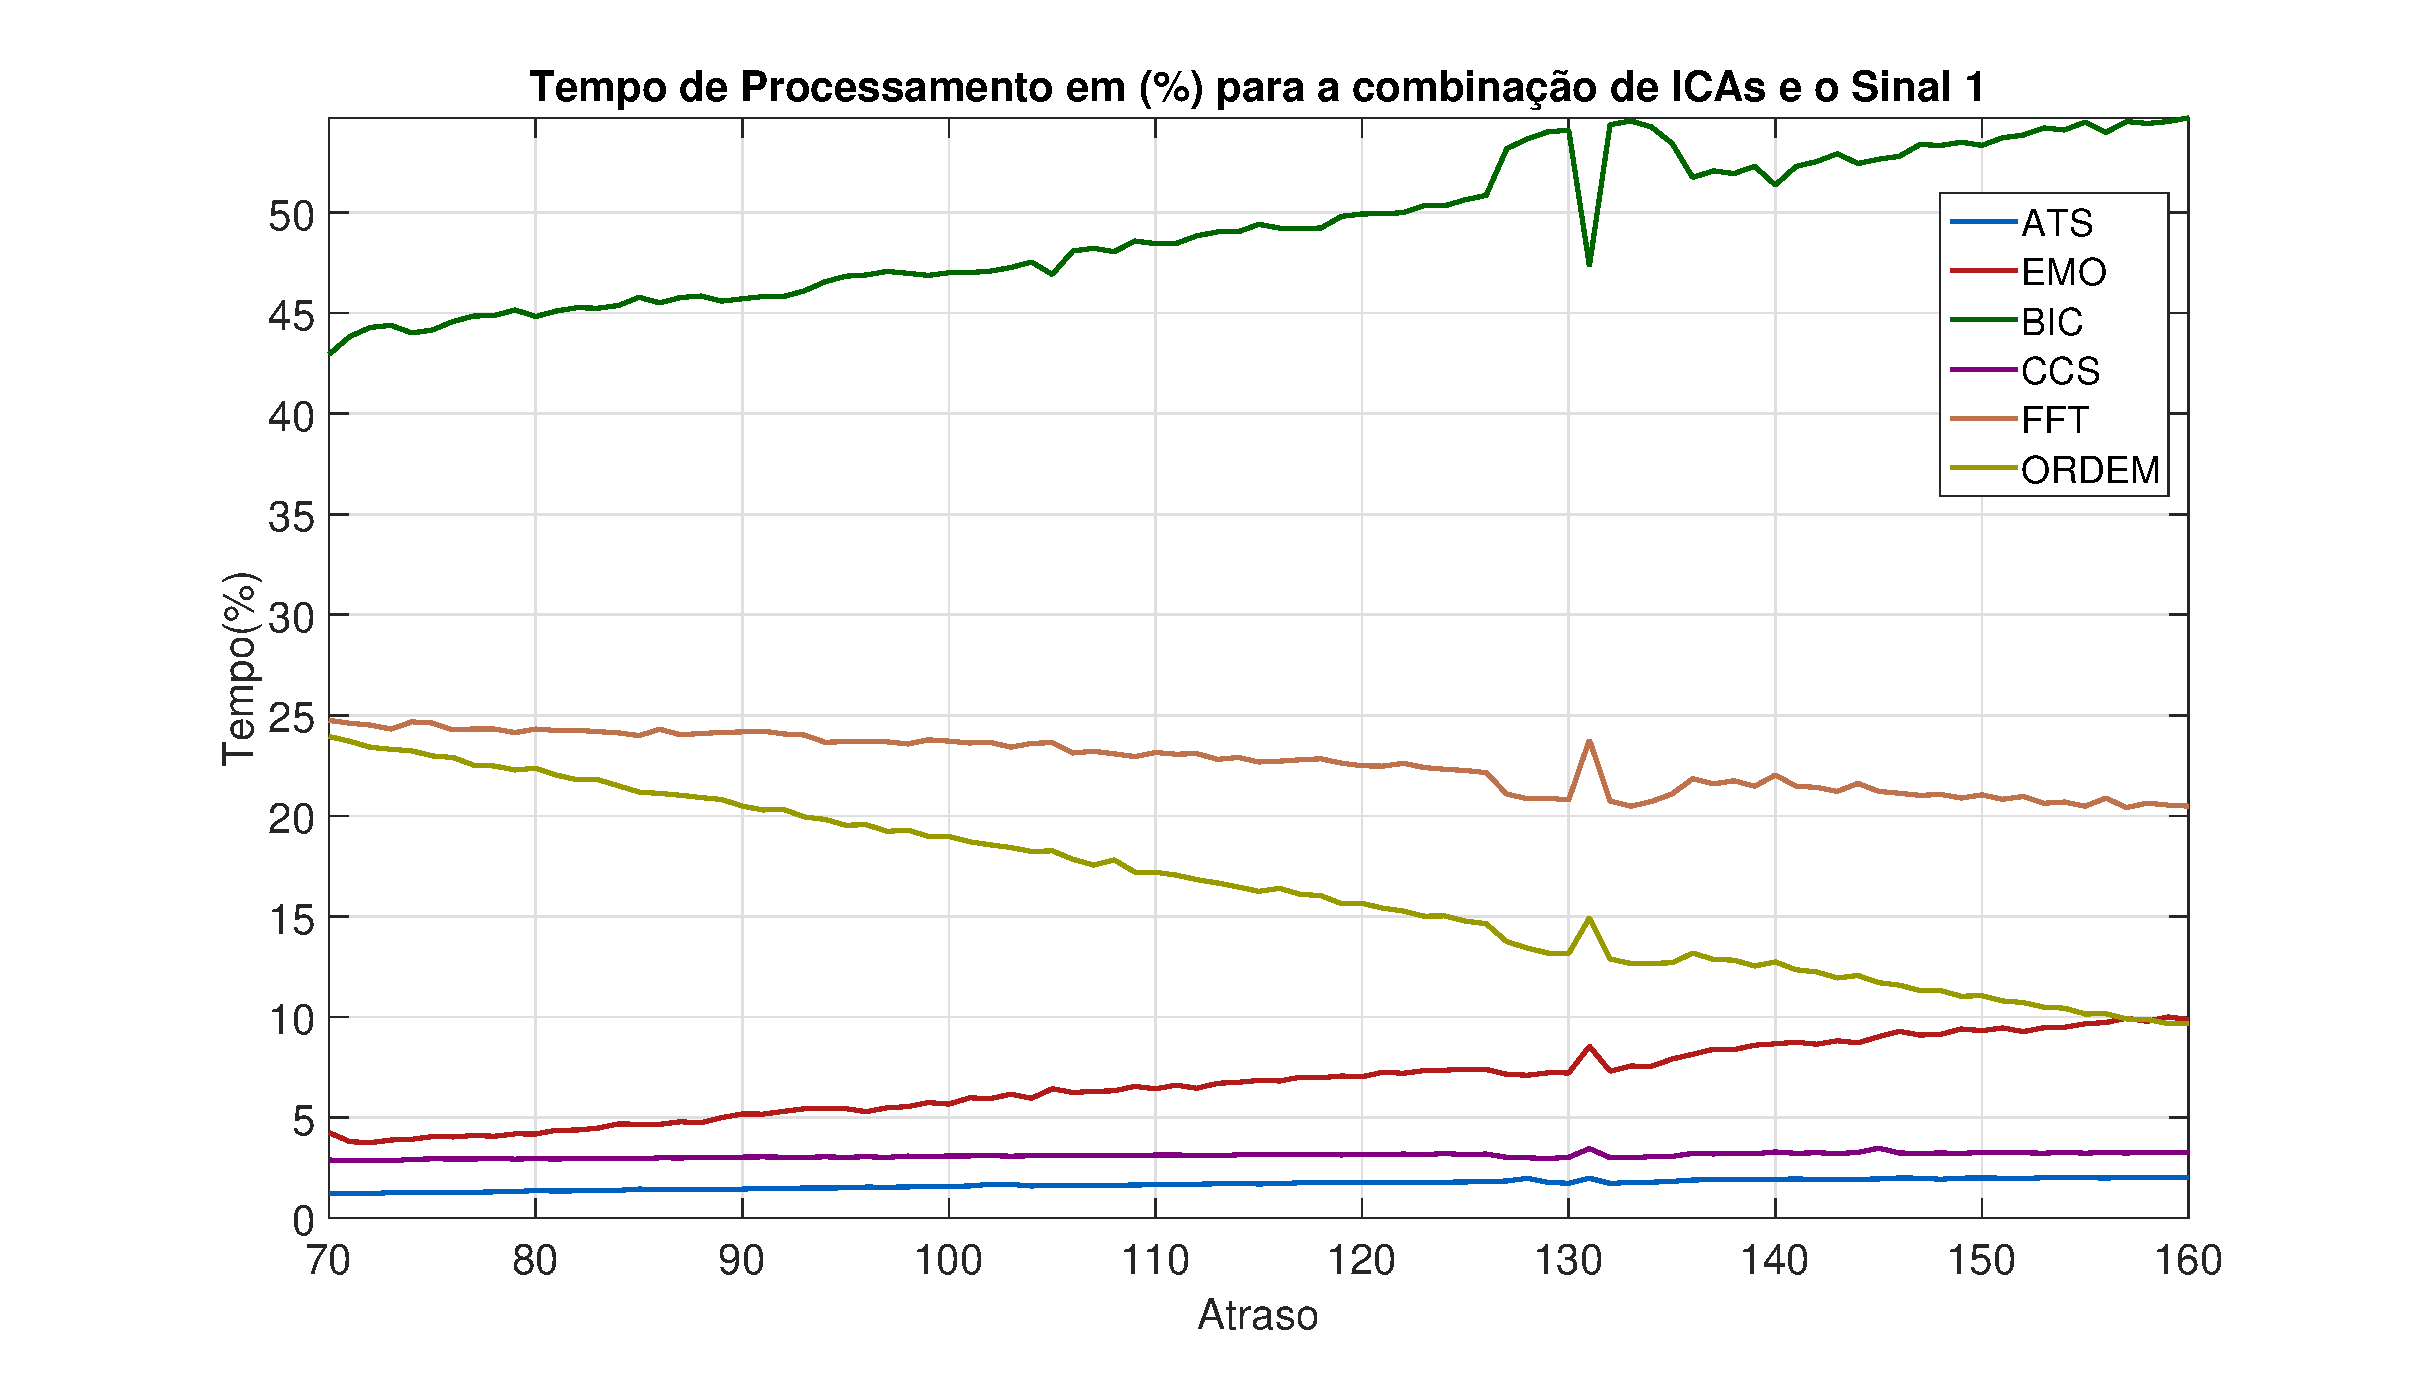
\includegraphics[scale=0.45]{imagens/ImagensParaOAnexo/TPPACombinacaoICASinal1.eps}
    \caption{TP em porcentagem dos testes para combinação de ICAs em S1.}
    \label{fig:TPCIAS1}    
    \end{center}
\end{figure}

\begin{figure}[!htb]
    \begin{center}
    \advance\leftskip -1.5cm
    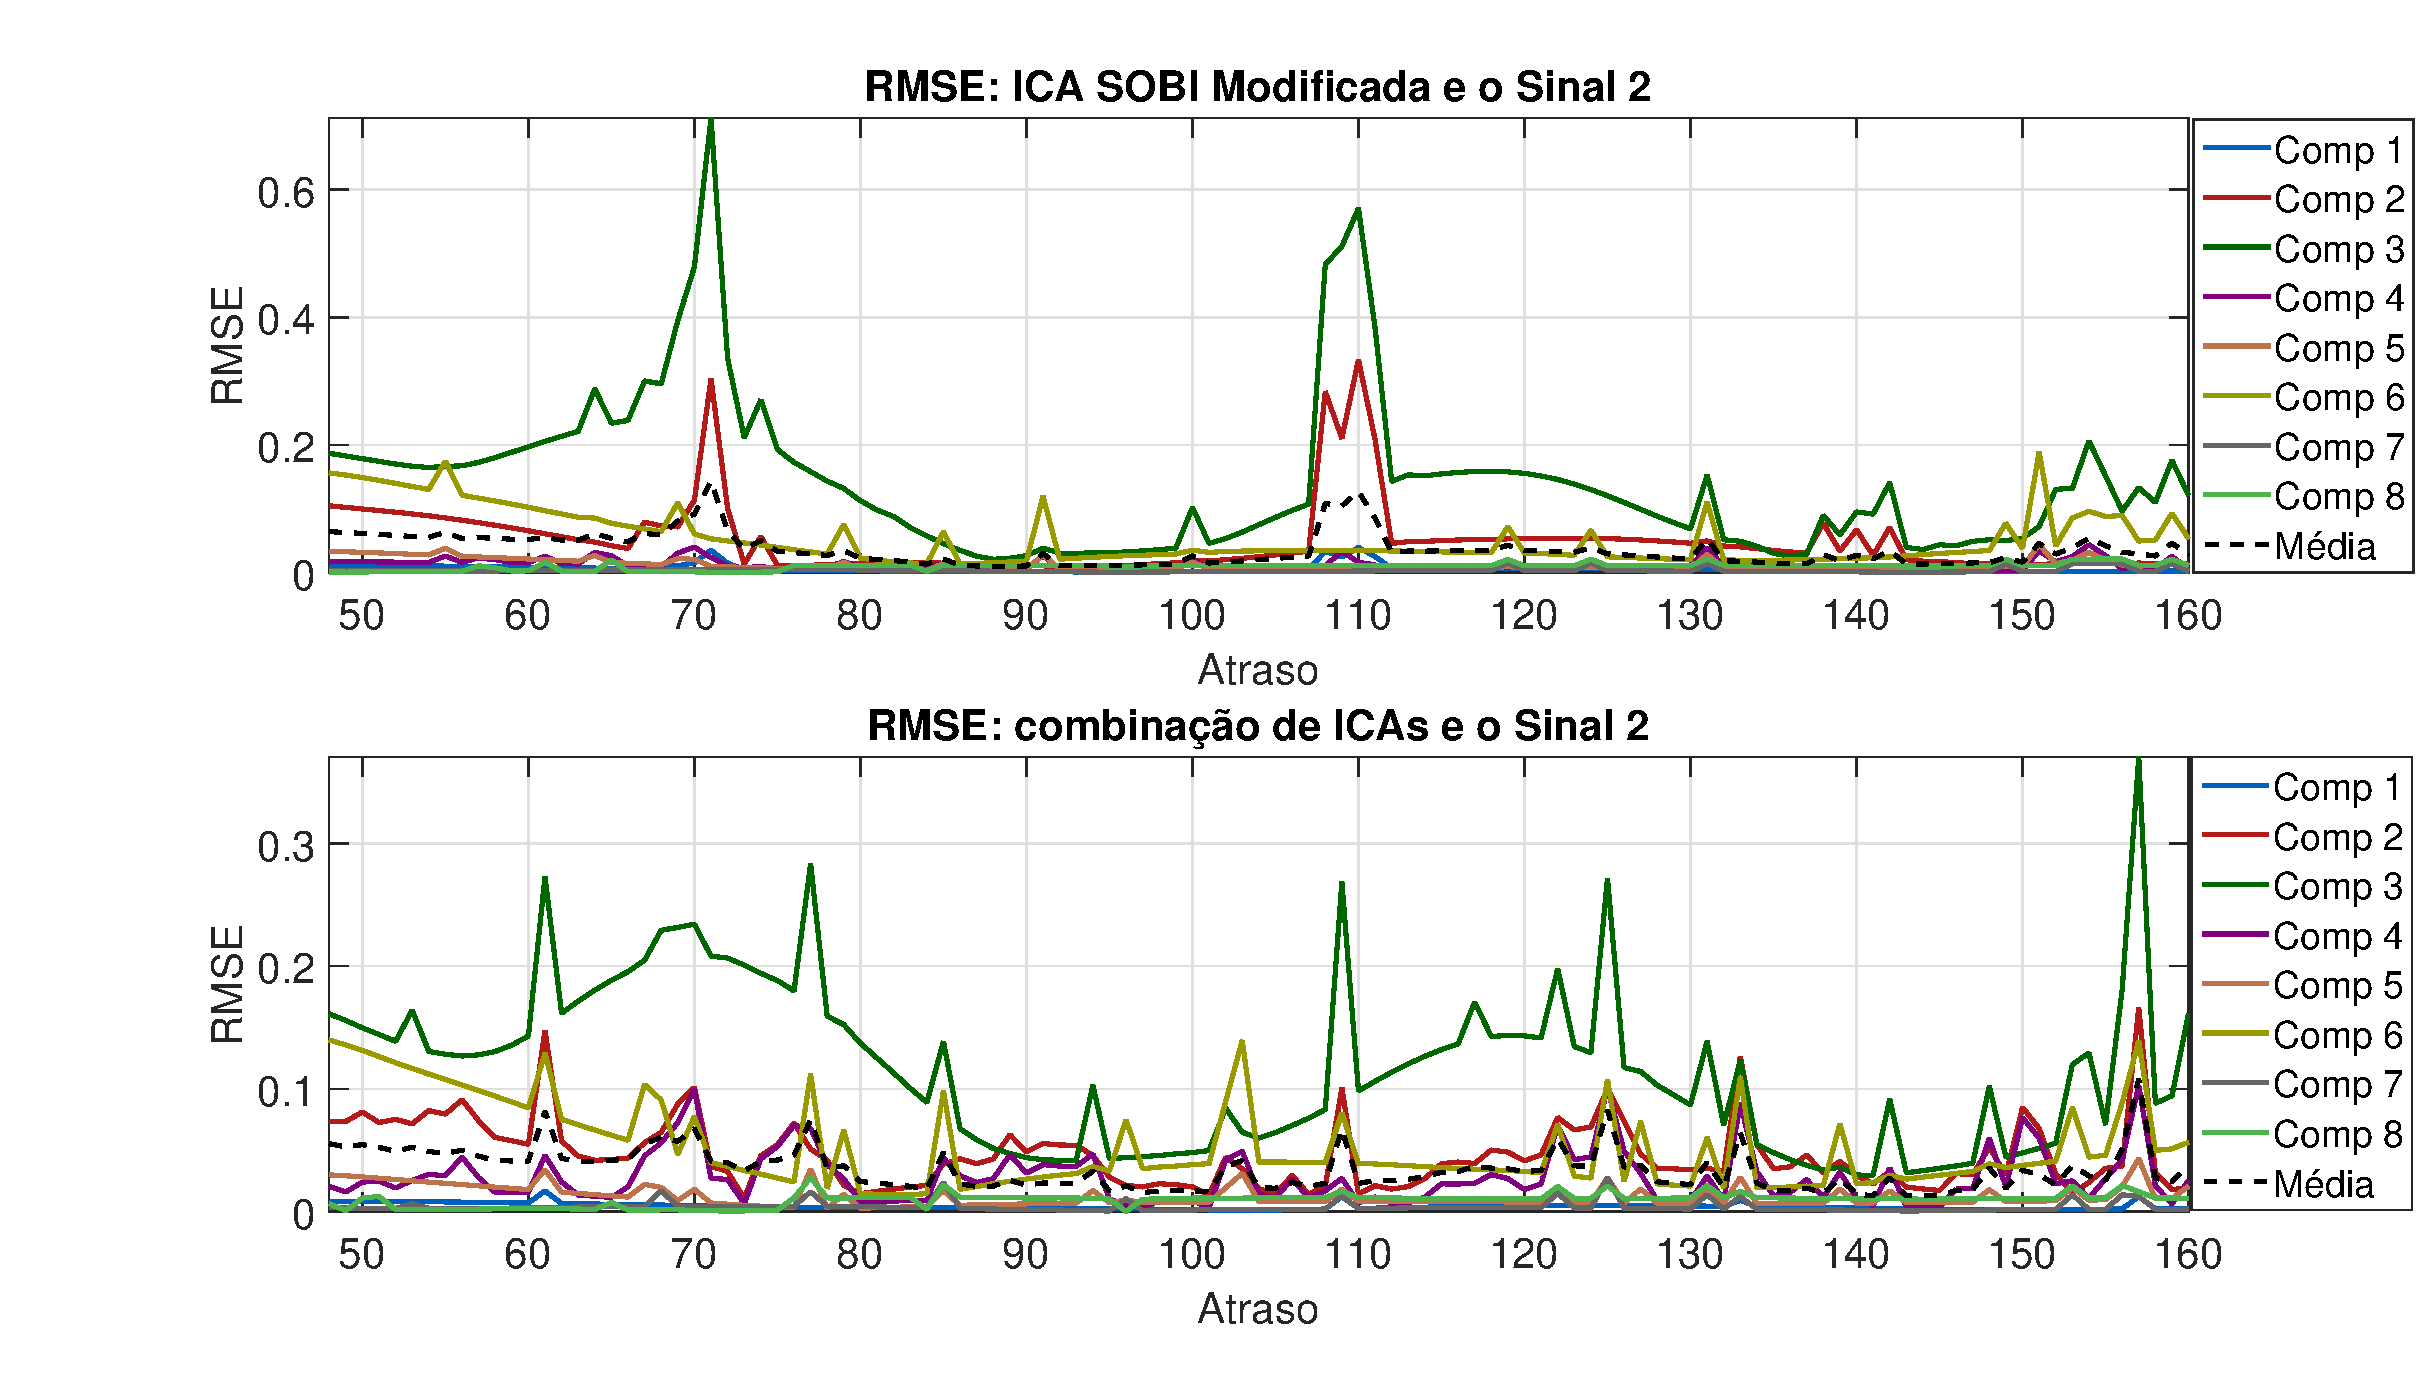
\includegraphics[scale=0.45]{imagens/ImagensParaOAnexo/RMSEcompATodasICAsSinal2.eps}
    \caption{RMSE por componente para as ICAs utilizadas e o S2.}
    \label{fig:RMSEAS2}    
    \end{center}
\end{figure}

\begin{figure}[!htb]
    \begin{center}
    \advance\leftskip -1.5cm
    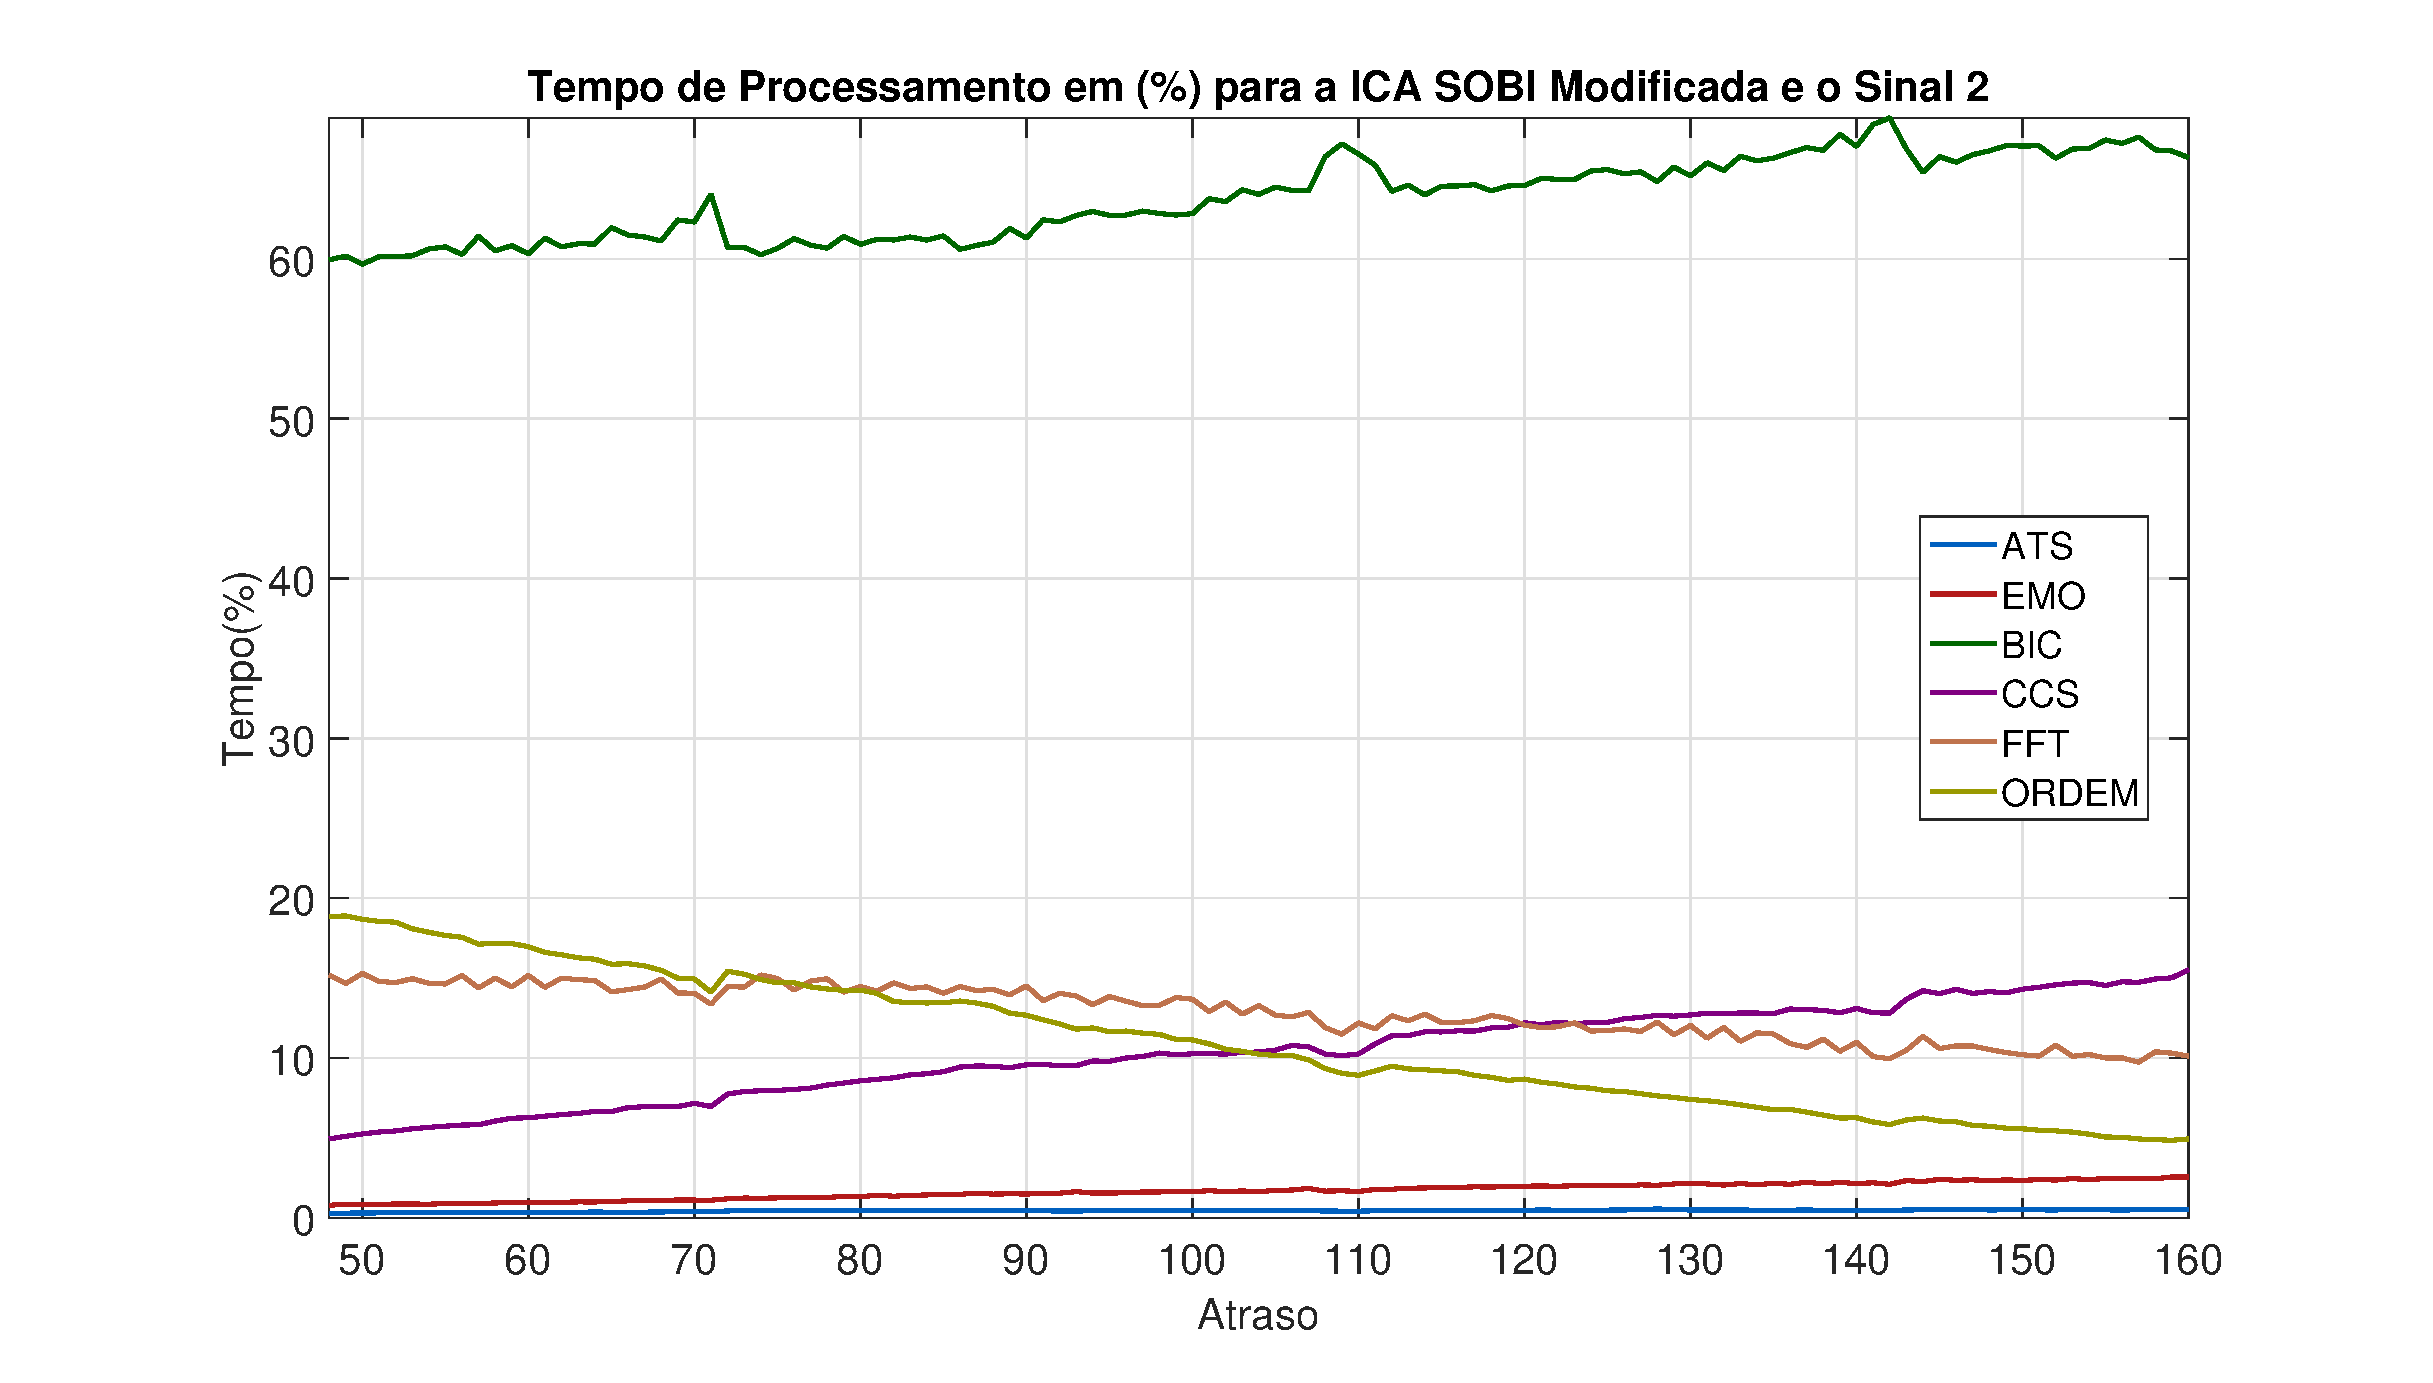
\includegraphics[scale=0.45]{imagens/ImagensParaOAnexo/TPPAICASOBImodSinal2.eps}
    \caption{TP em porcentagem dos testes para ICA SOBI modificado em S2.}
    \label{fig:TPSMAS2}    
    \end{center}
\end{figure}

\begin{figure}[!htb]
    \begin{center}
    \advance\leftskip -1.5cm
    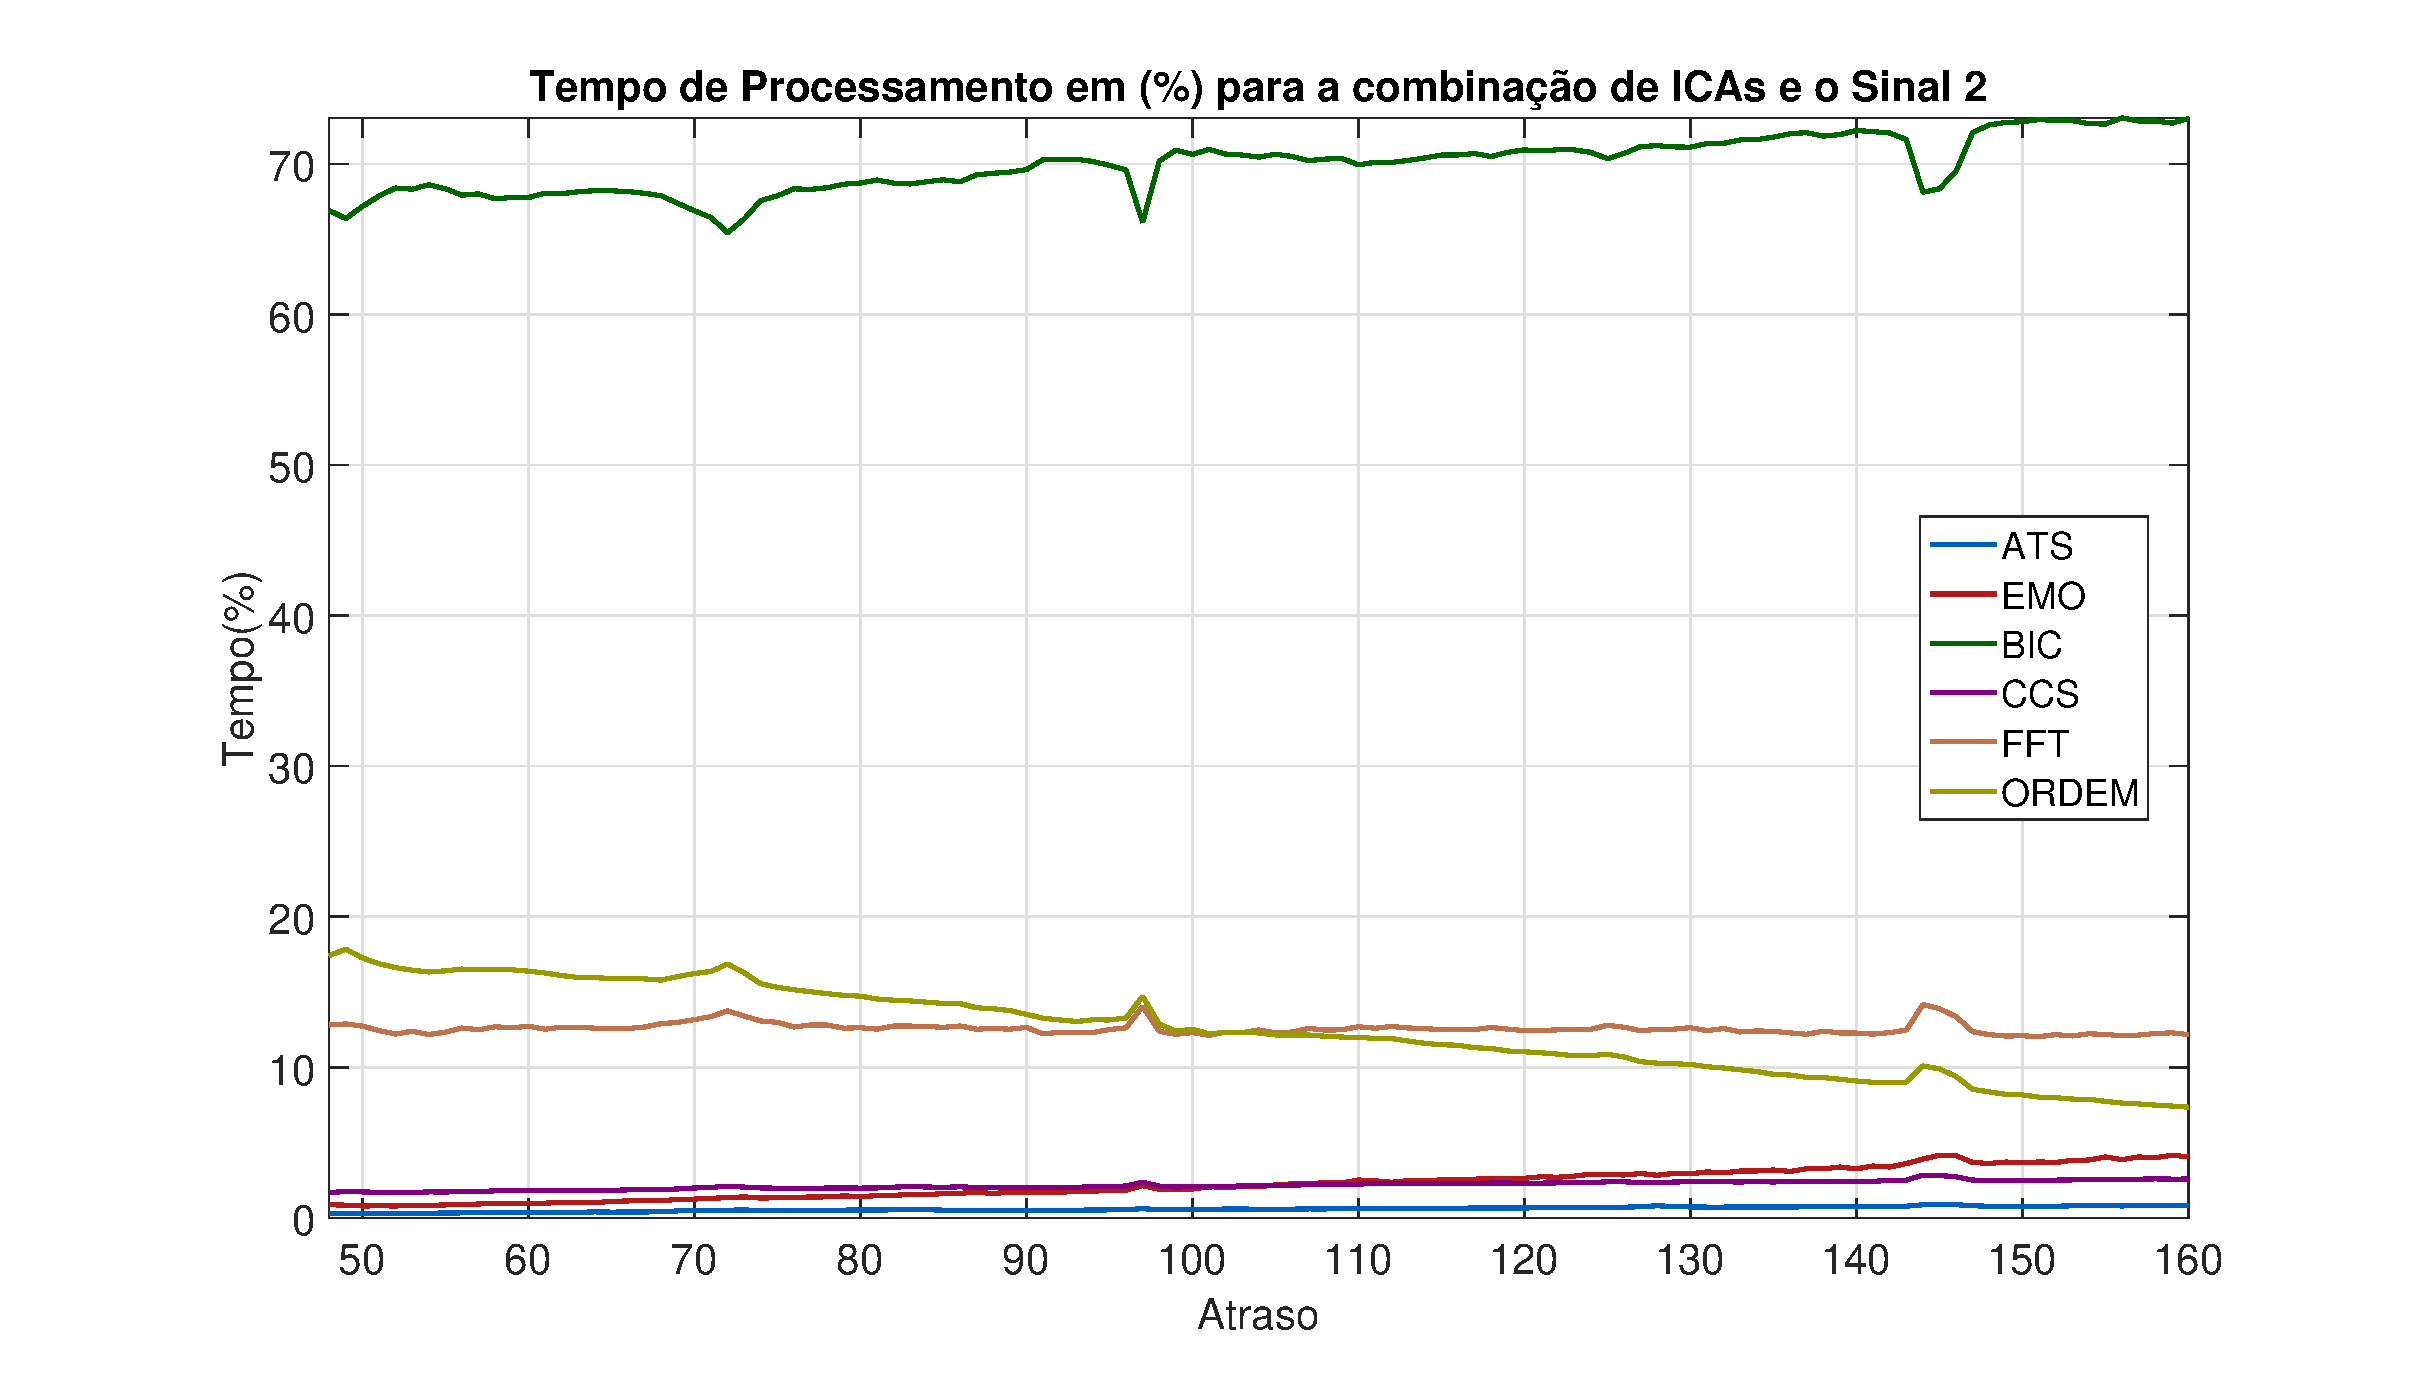
\includegraphics[scale=0.45]{imagens/ImagensParaOAnexo/TPPACombinacaoICASinal2.eps}
    \caption{TP em porcentagem dos testes para combinação de ICAs em S2.}
    \label{fig:TPCIAS2}    
    \end{center}
\end{figure}

\begin{figure}[!htb]
    \begin{center}
    \advance\leftskip -1.5cm
    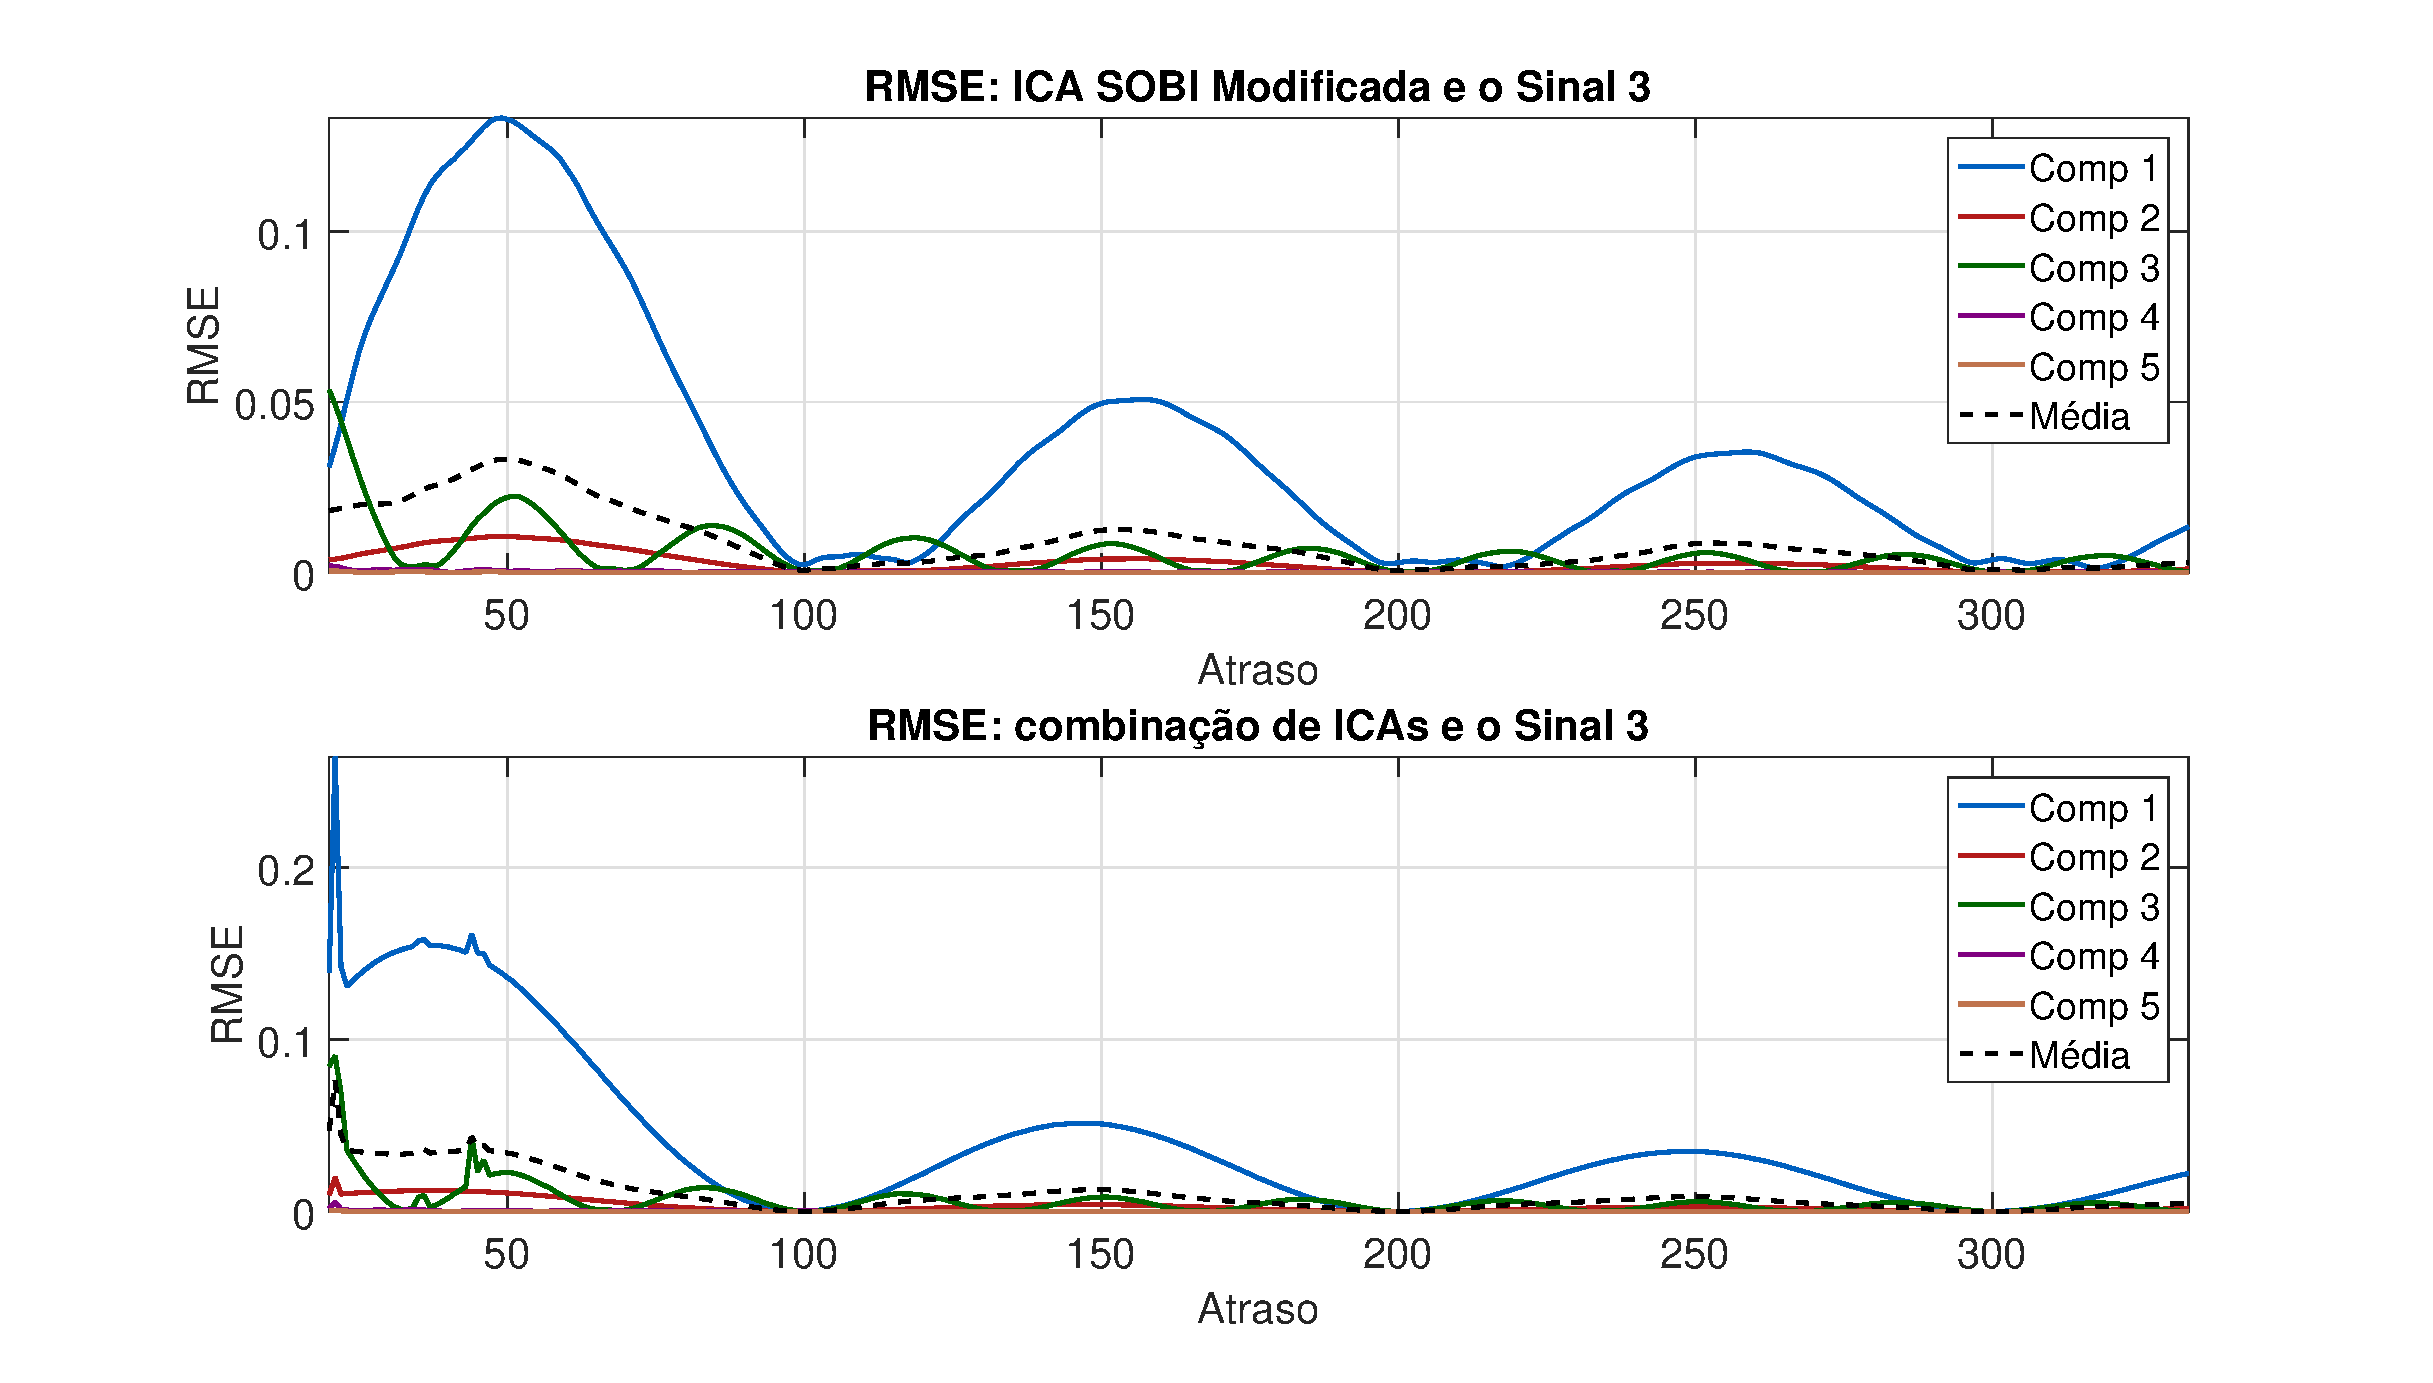
\includegraphics[scale=0.45]{imagens/ImagensParaOAnexo/RMSEcompATodasICAsSinal3.eps}
    \caption{RMSE por componente para as ICAs utilizadas e o S3.}
    \label{fig:RMSEAS3}    
    \end{center}
\end{figure}

\begin{figure}[!htb]
    \begin{center}
    \advance\leftskip -1.5cm
    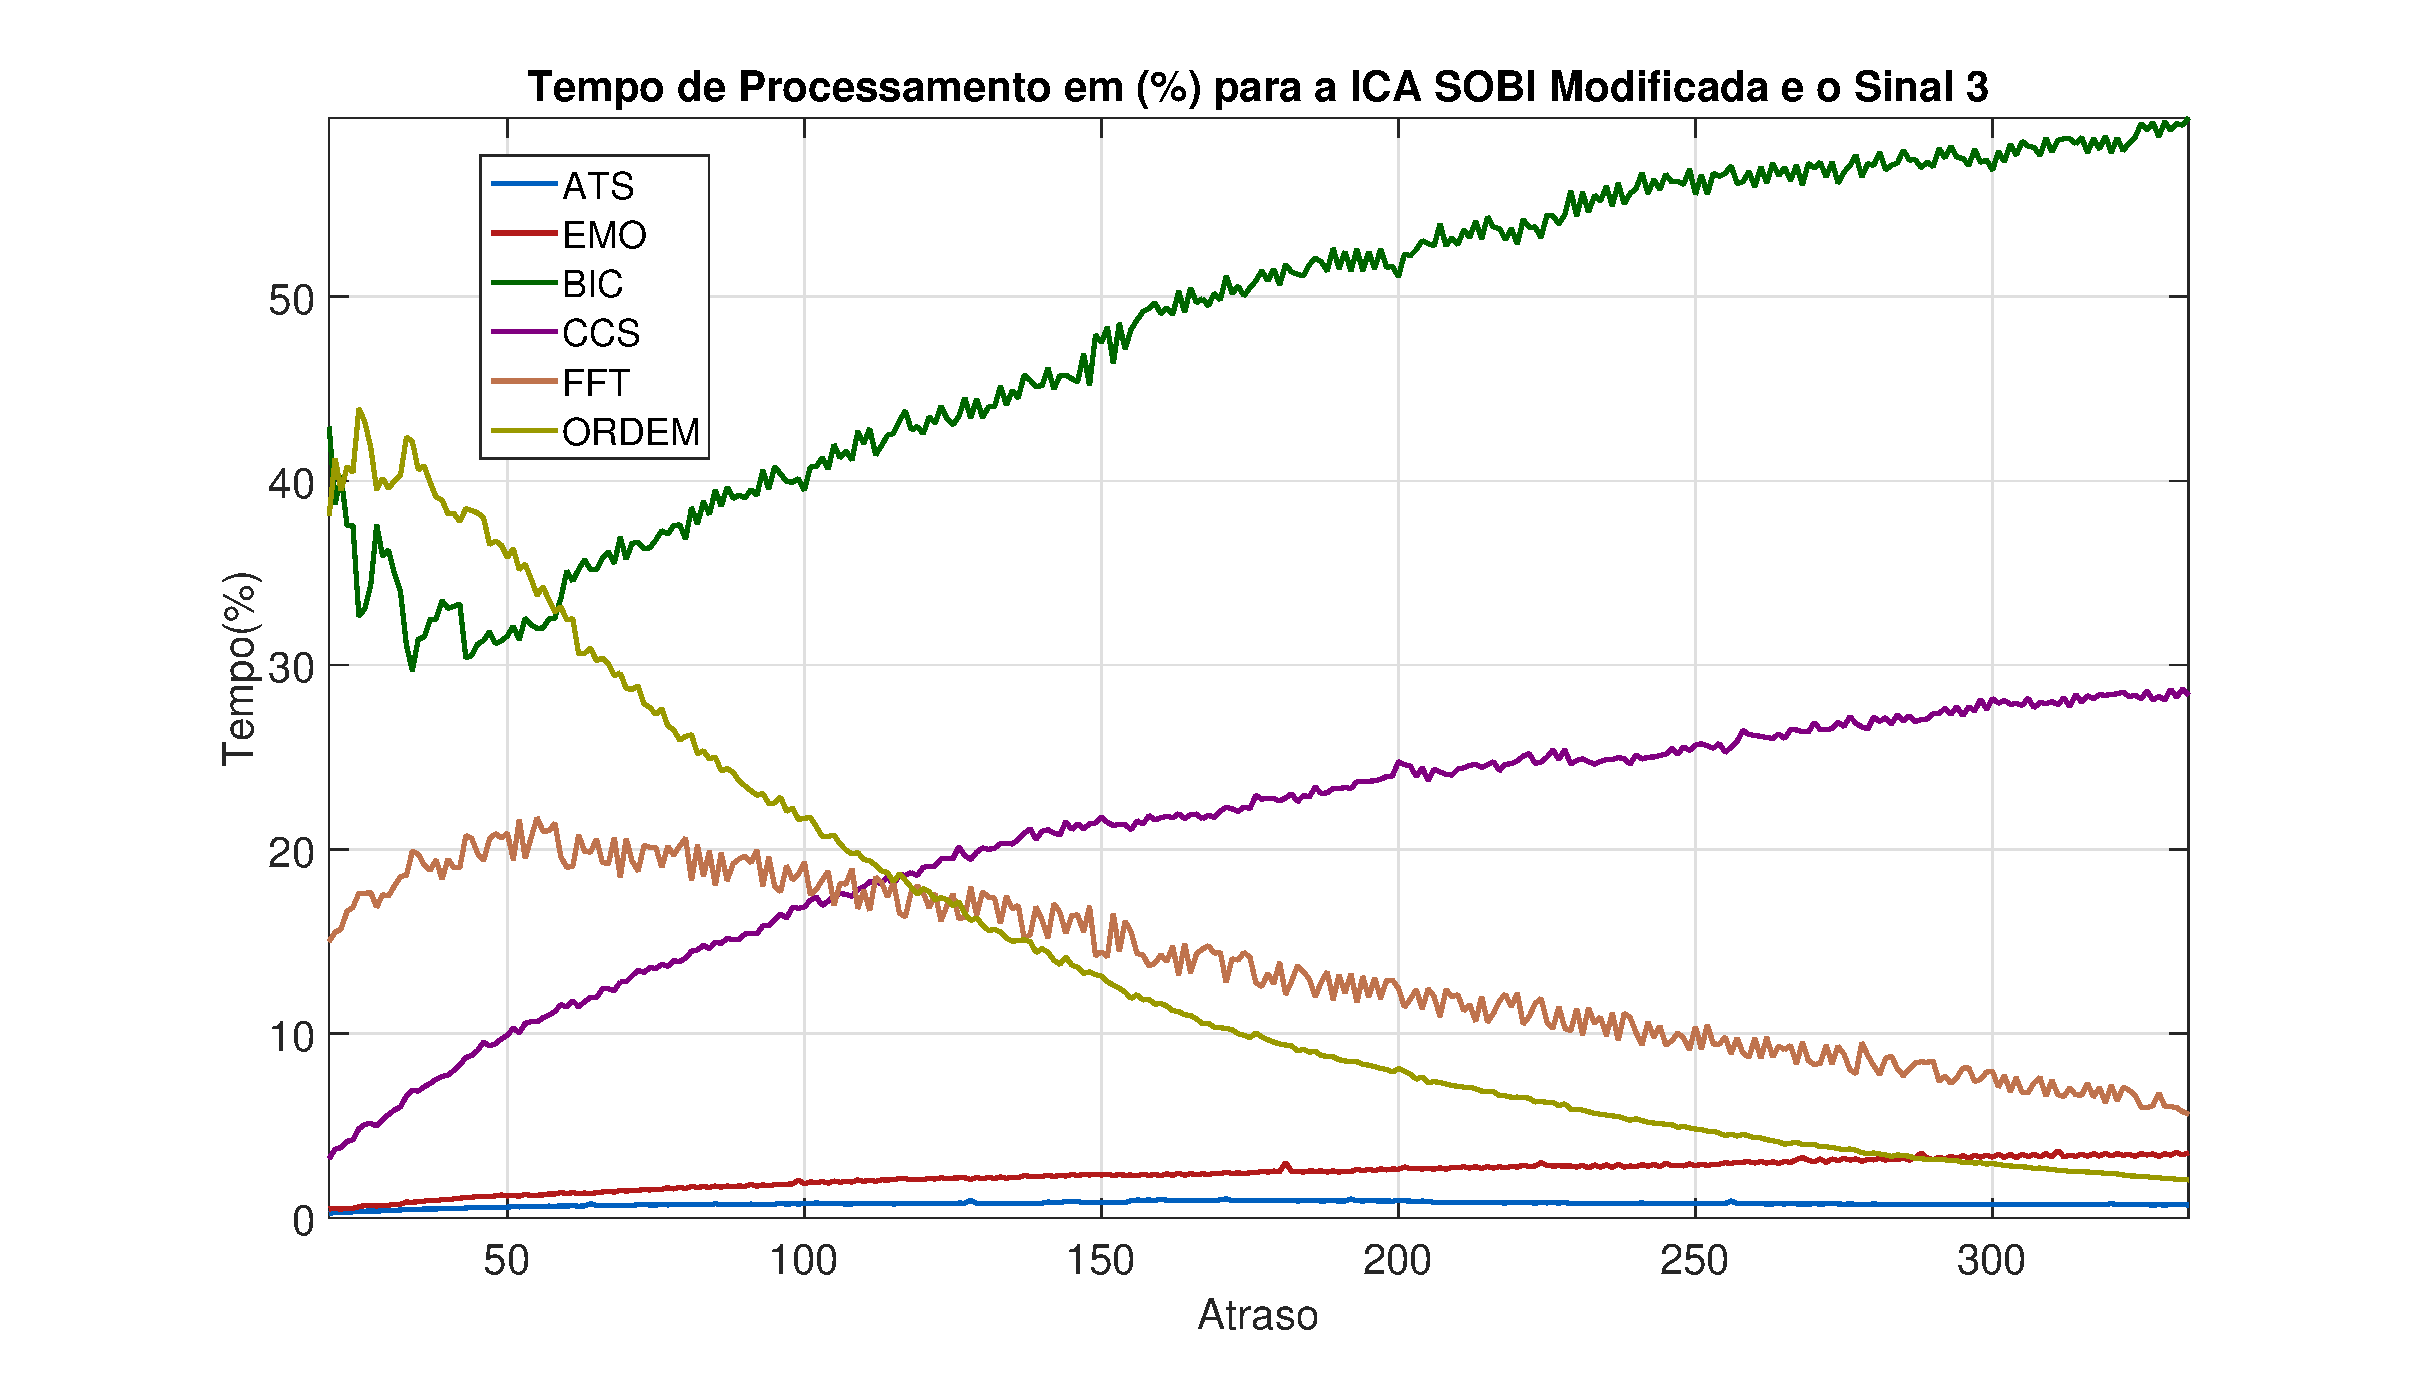
\includegraphics[scale=0.45]{imagens/ImagensParaOAnexo/TPPAICASOBImodSinal3.eps}
    \caption{TP em porcentagem dos testes para ICA SOBI modificado em S3.}
    \label{fig:TPSMAS3}    
    \end{center}
\end{figure}

\begin{figure}[!htb]
    \begin{center}
    \advance\leftskip -1.5cm
    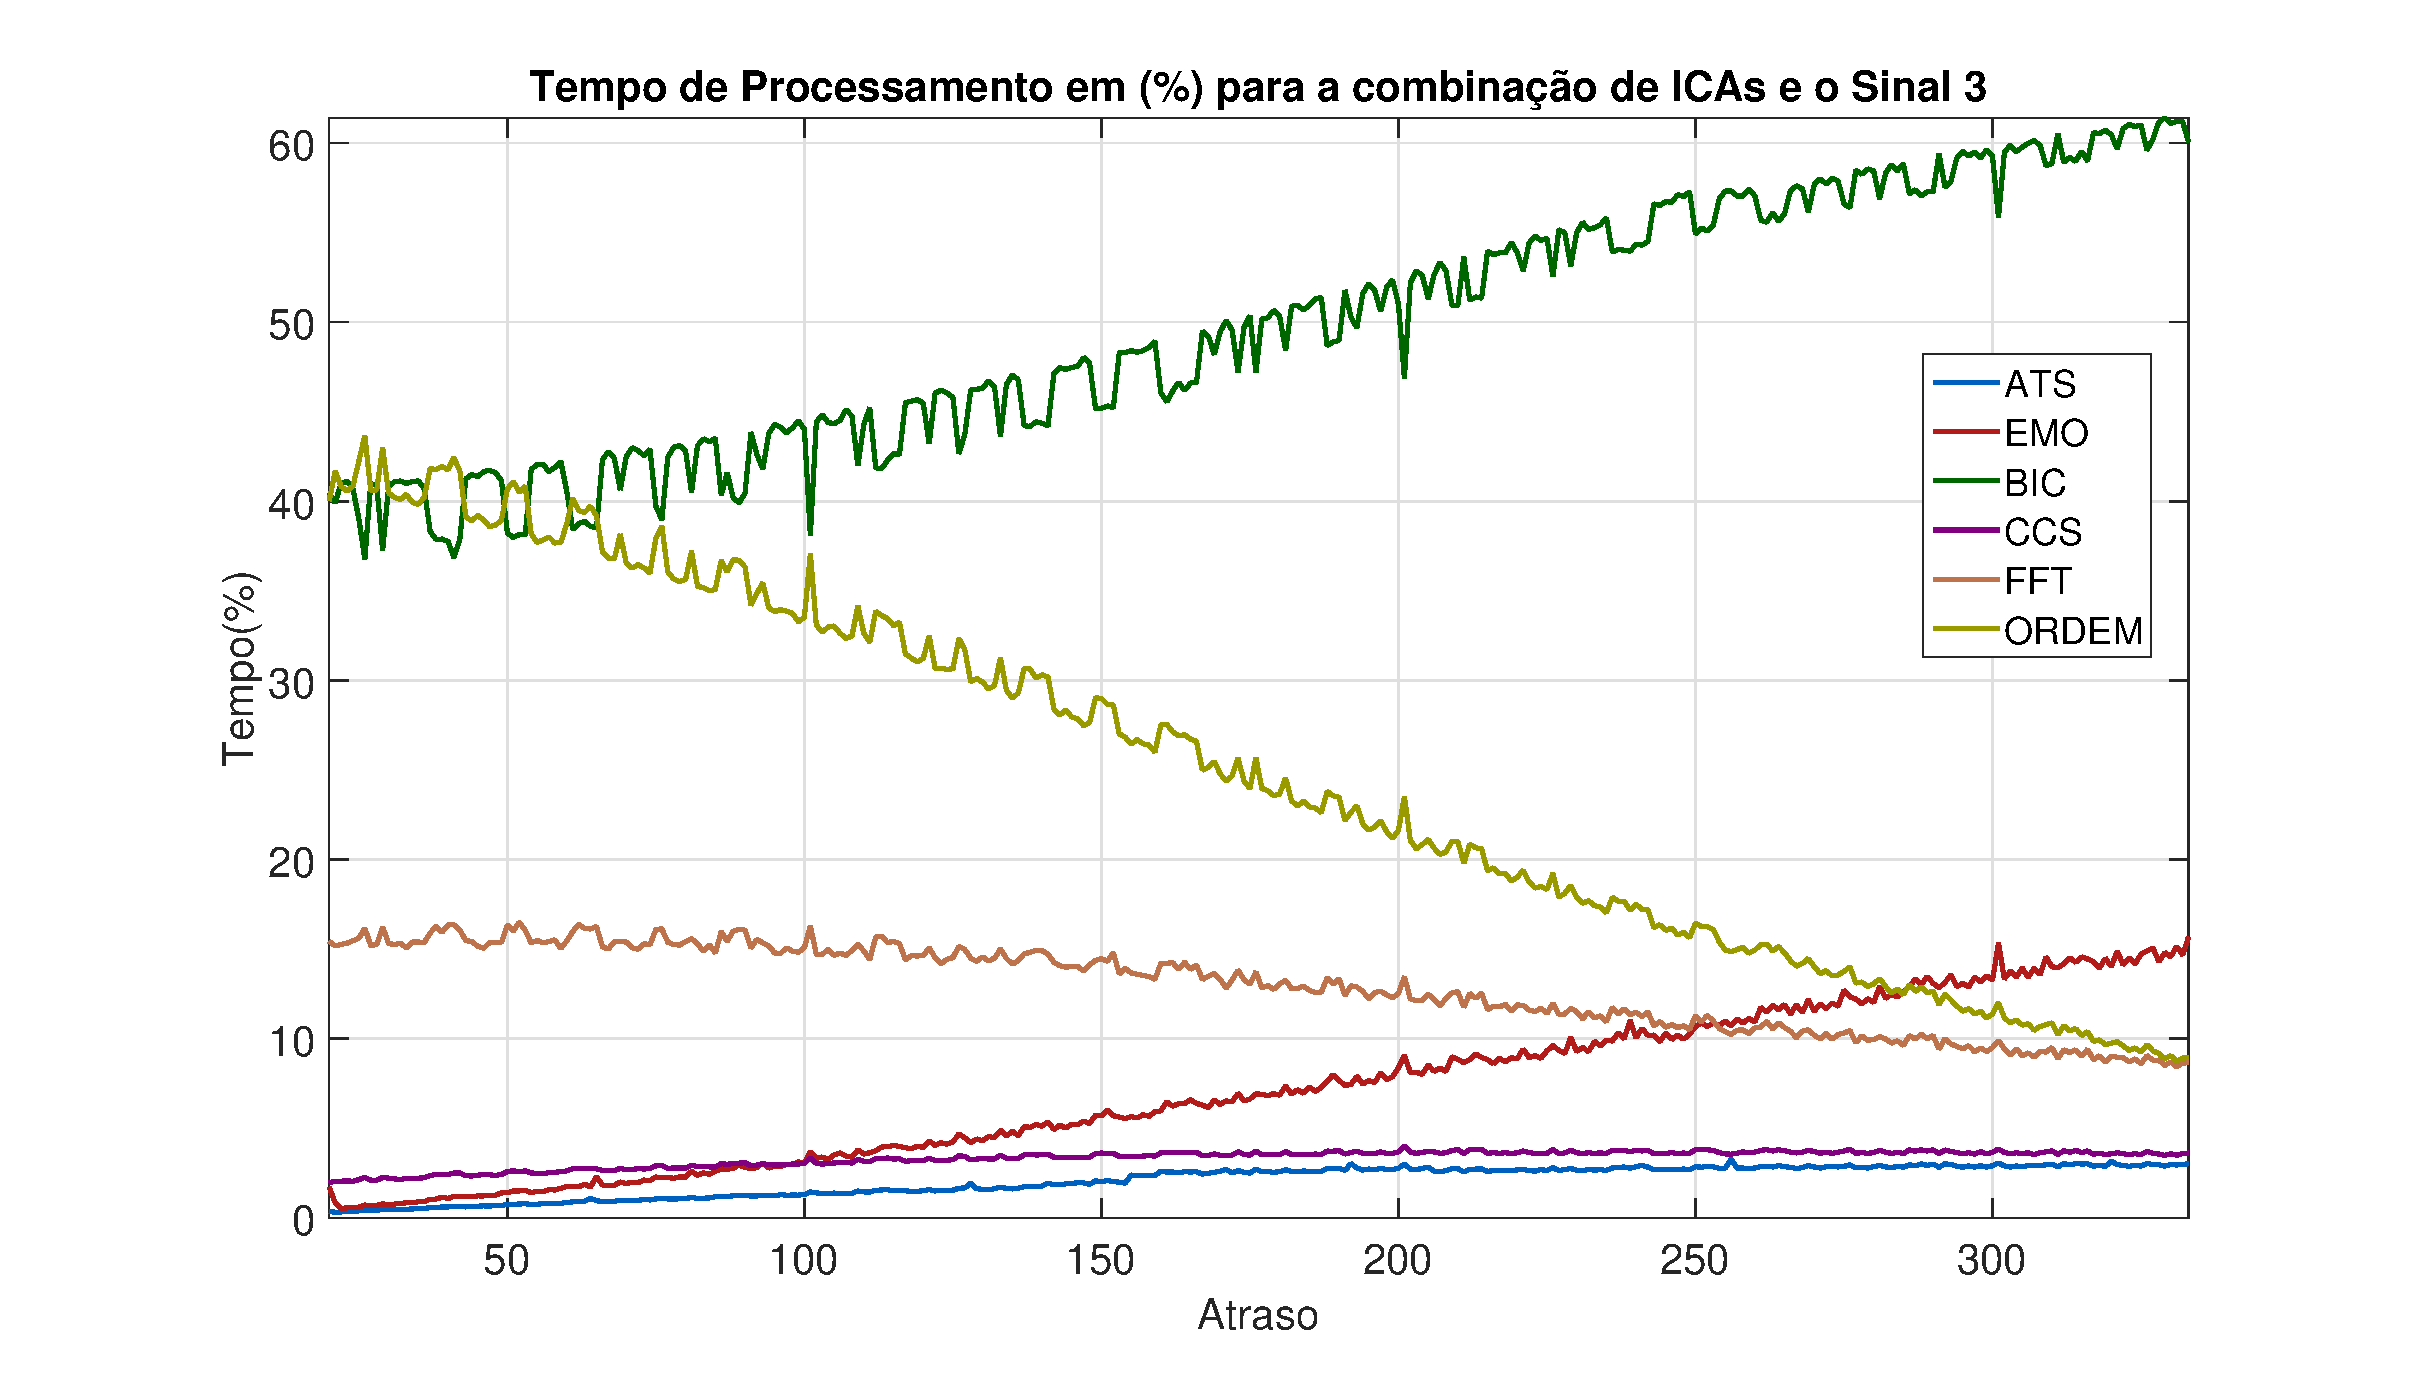
\includegraphics[scale=0.45]{imagens/ImagensParaOAnexo/TPPACombinacaoICASinal3.eps}
    \caption{TP em porcentagem dos testes para combinação de ICAs em S3.}
    \label{fig:TPCIAS3}    
    \end{center}
\end{figure}

\begin{figure}[!htb]
    \begin{center}
    \advance\leftskip -1.5cm
    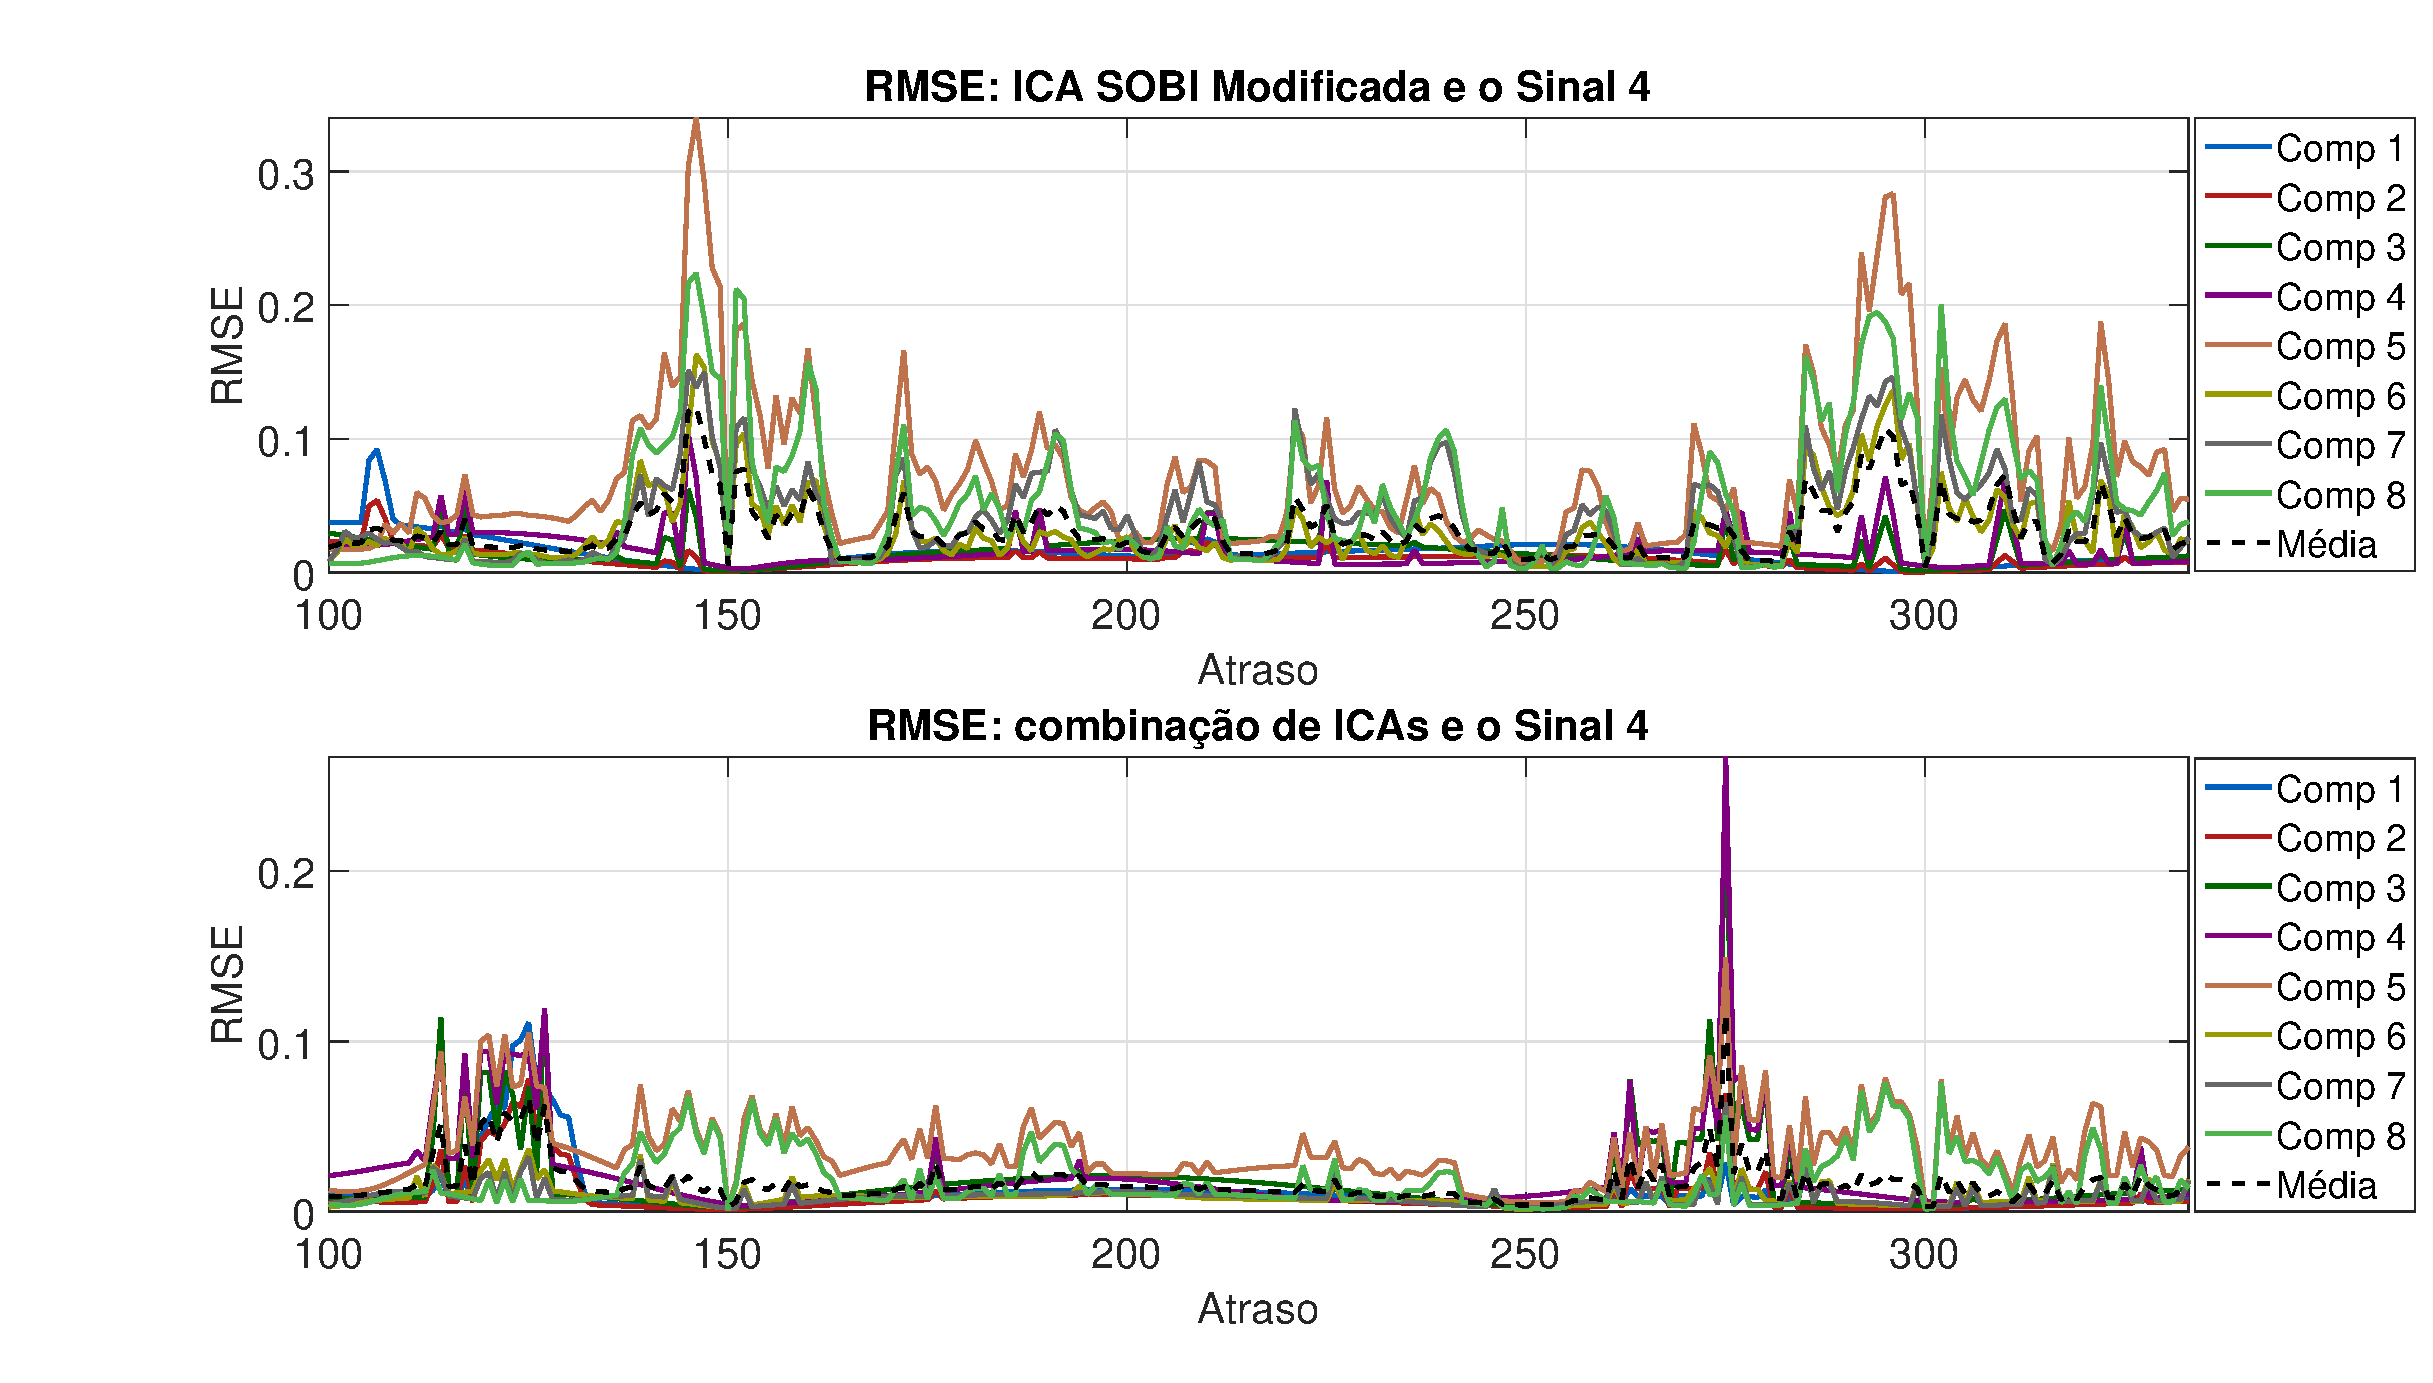
\includegraphics[scale=0.45]{imagens/ImagensParaOAnexo/RMSEcompATodasICAsSinal4.eps}
    \caption{RMSE por componente para as ICAs utilizadas e o S4.}
    \label{fig:RMSEAS4}    
    \end{center}
\end{figure}

\begin{figure}[!htb]
    \begin{center}
    \advance\leftskip -1.5cm
    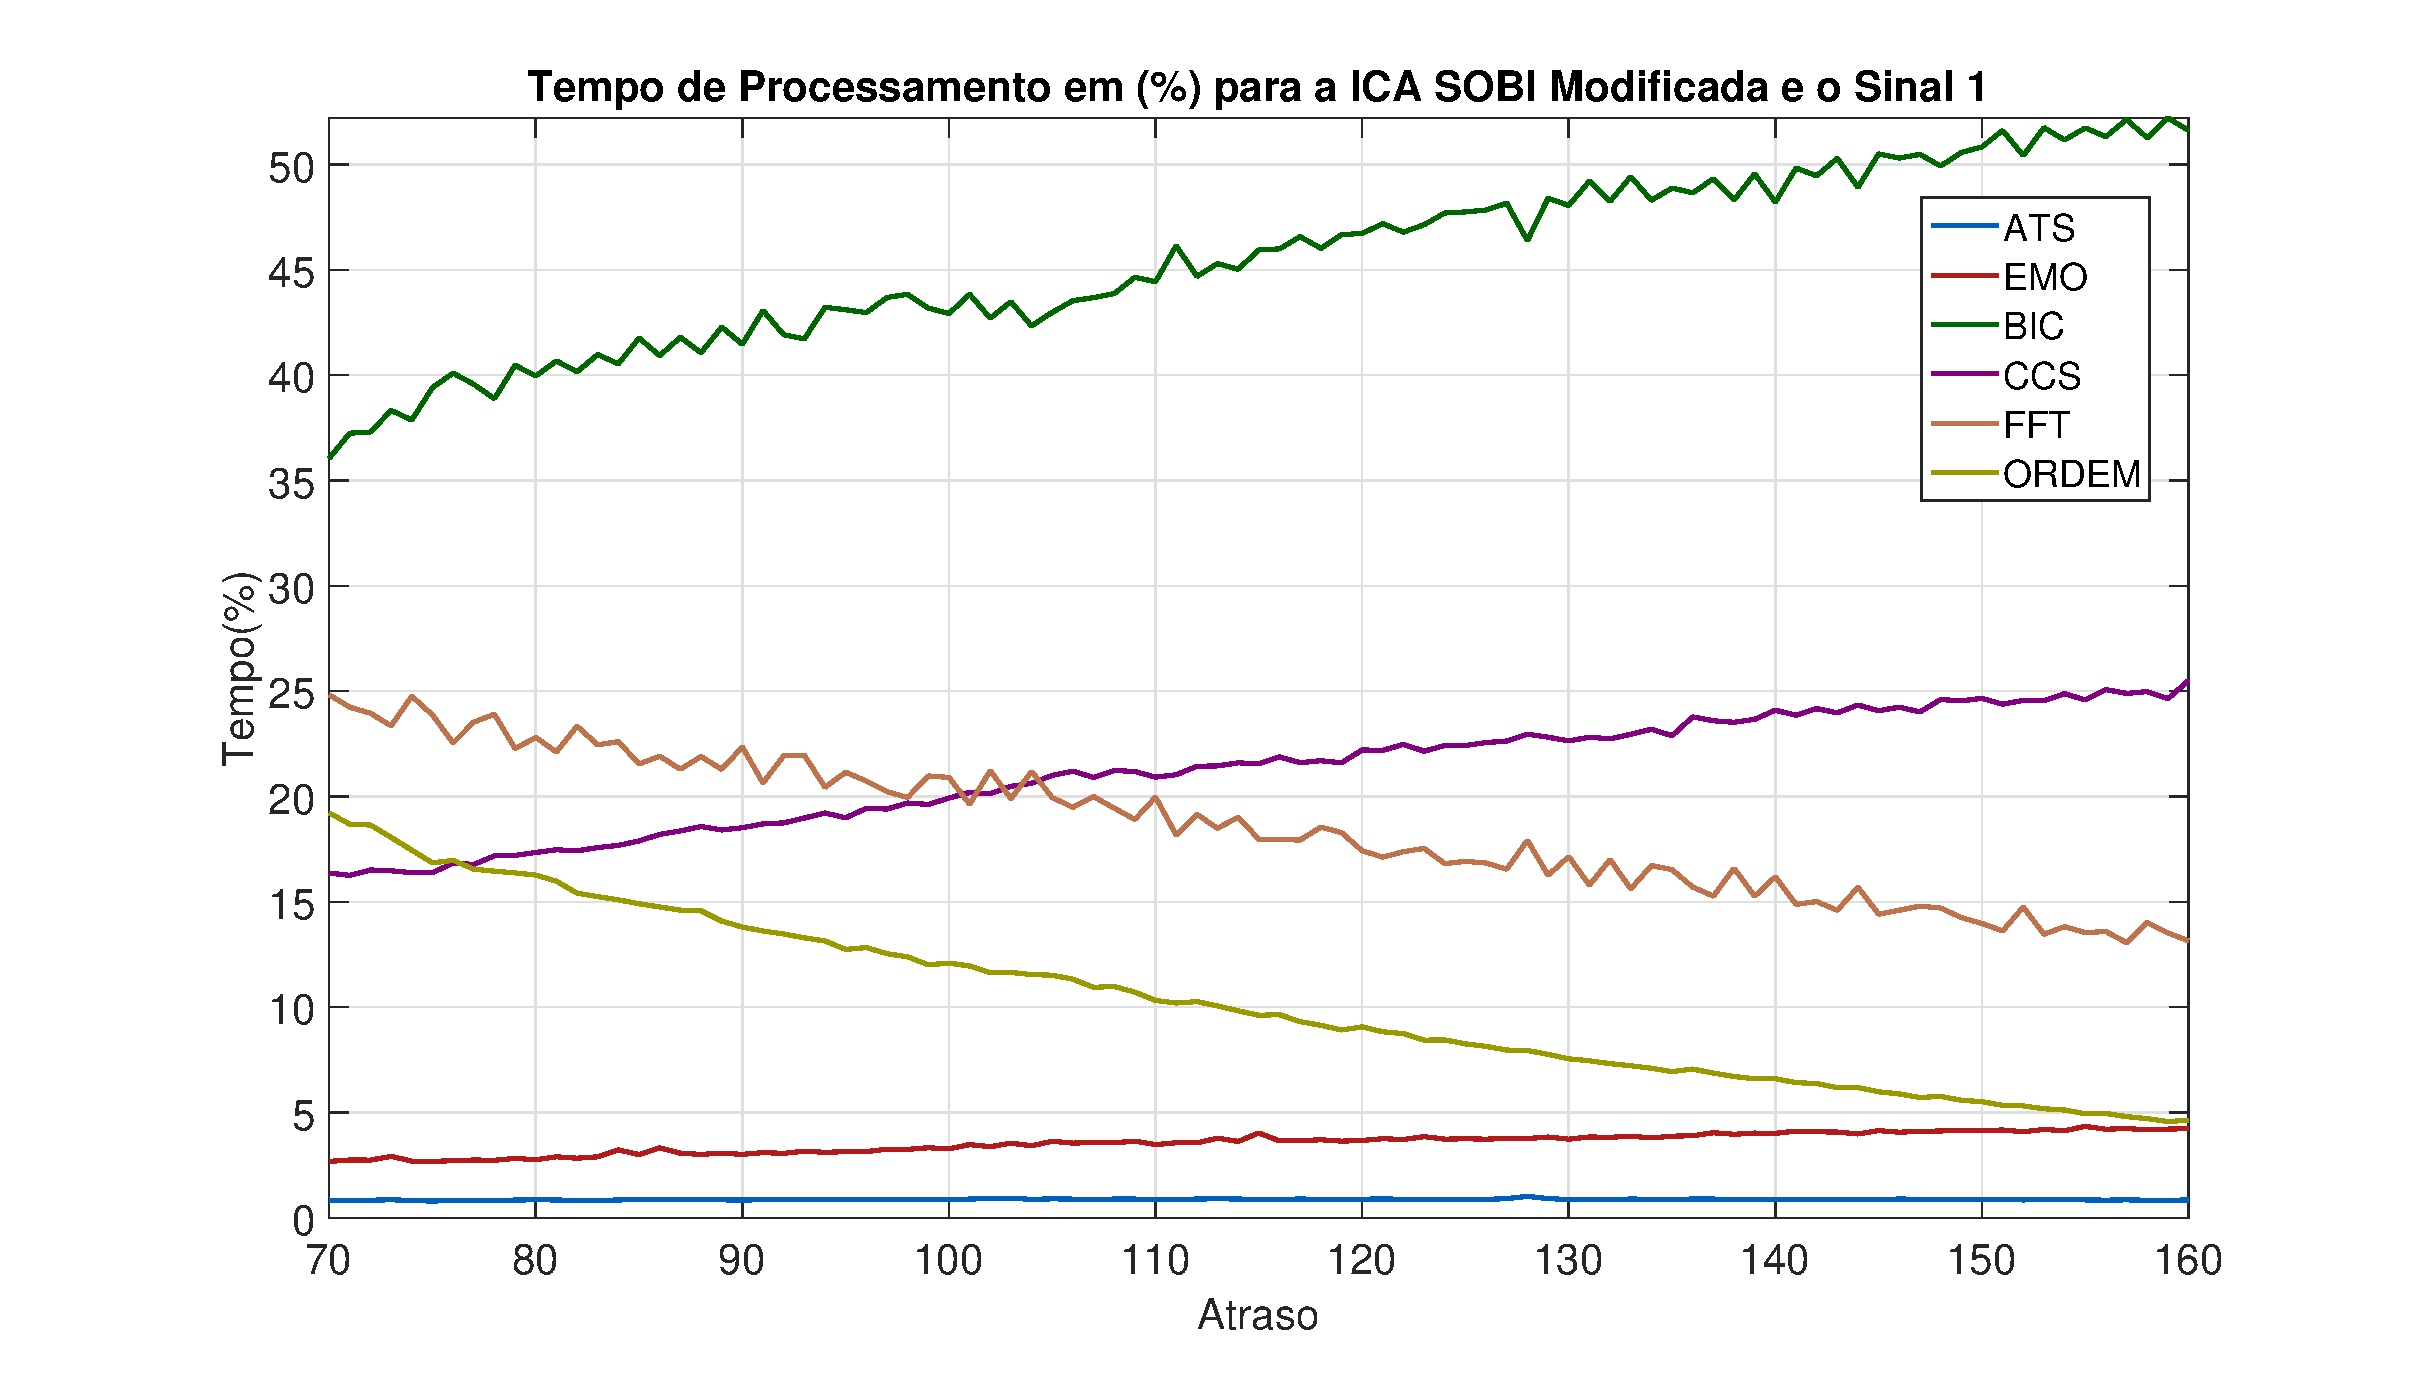
\includegraphics[scale=0.45]{imagens/ImagensParaOAnexo/TPPAICASOBImodSinal1.eps}
    \caption{TP em porcentagem dos testes para ICA SOBI modificado em S4.}
    \label{fig:TPSMAS4}    
    \end{center}
\end{figure}

\begin{figure}[!htb]
    \begin{center}
    \advance\leftskip -1.5cm
    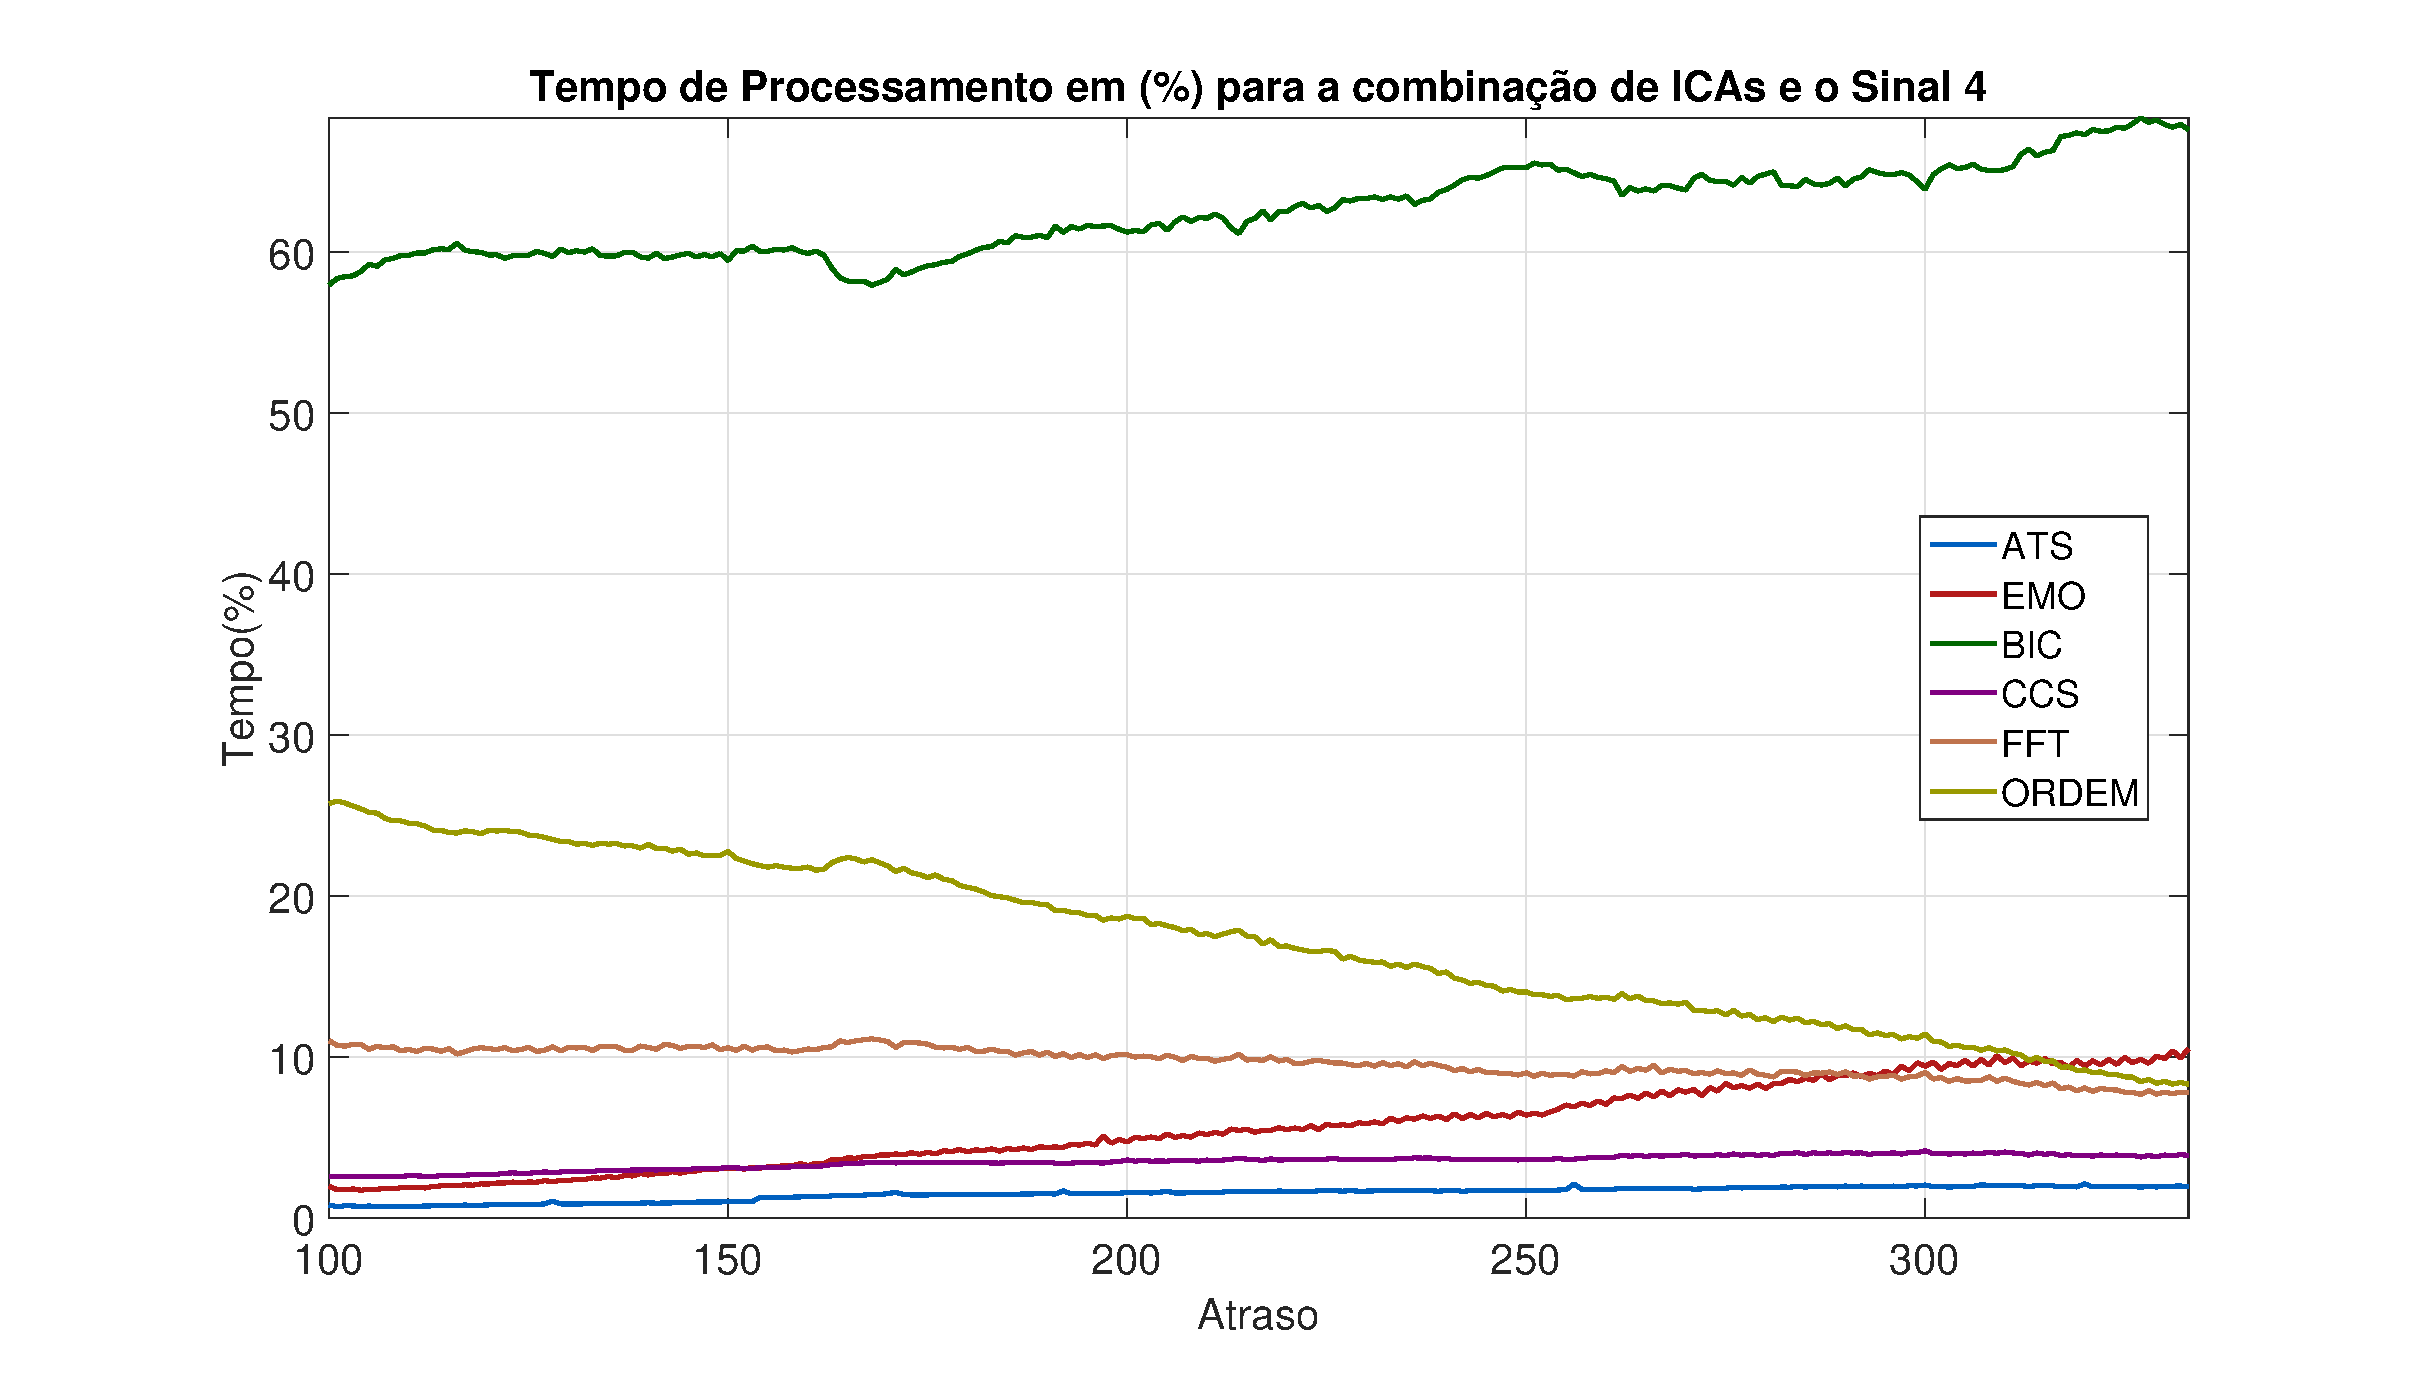
\includegraphics[scale=0.45]{imagens/ImagensParaOAnexo/TPPACombinacaoICASinal4.eps}
    \caption{TP em porcentagem dos testes para combinação de ICAs em S4.}
    \label{fig:TPCIAS4}    
    \end{center}
\end{figure}

\begin{figure}[!htb]
    \begin{center}
    \advance\leftskip -1.5cm
    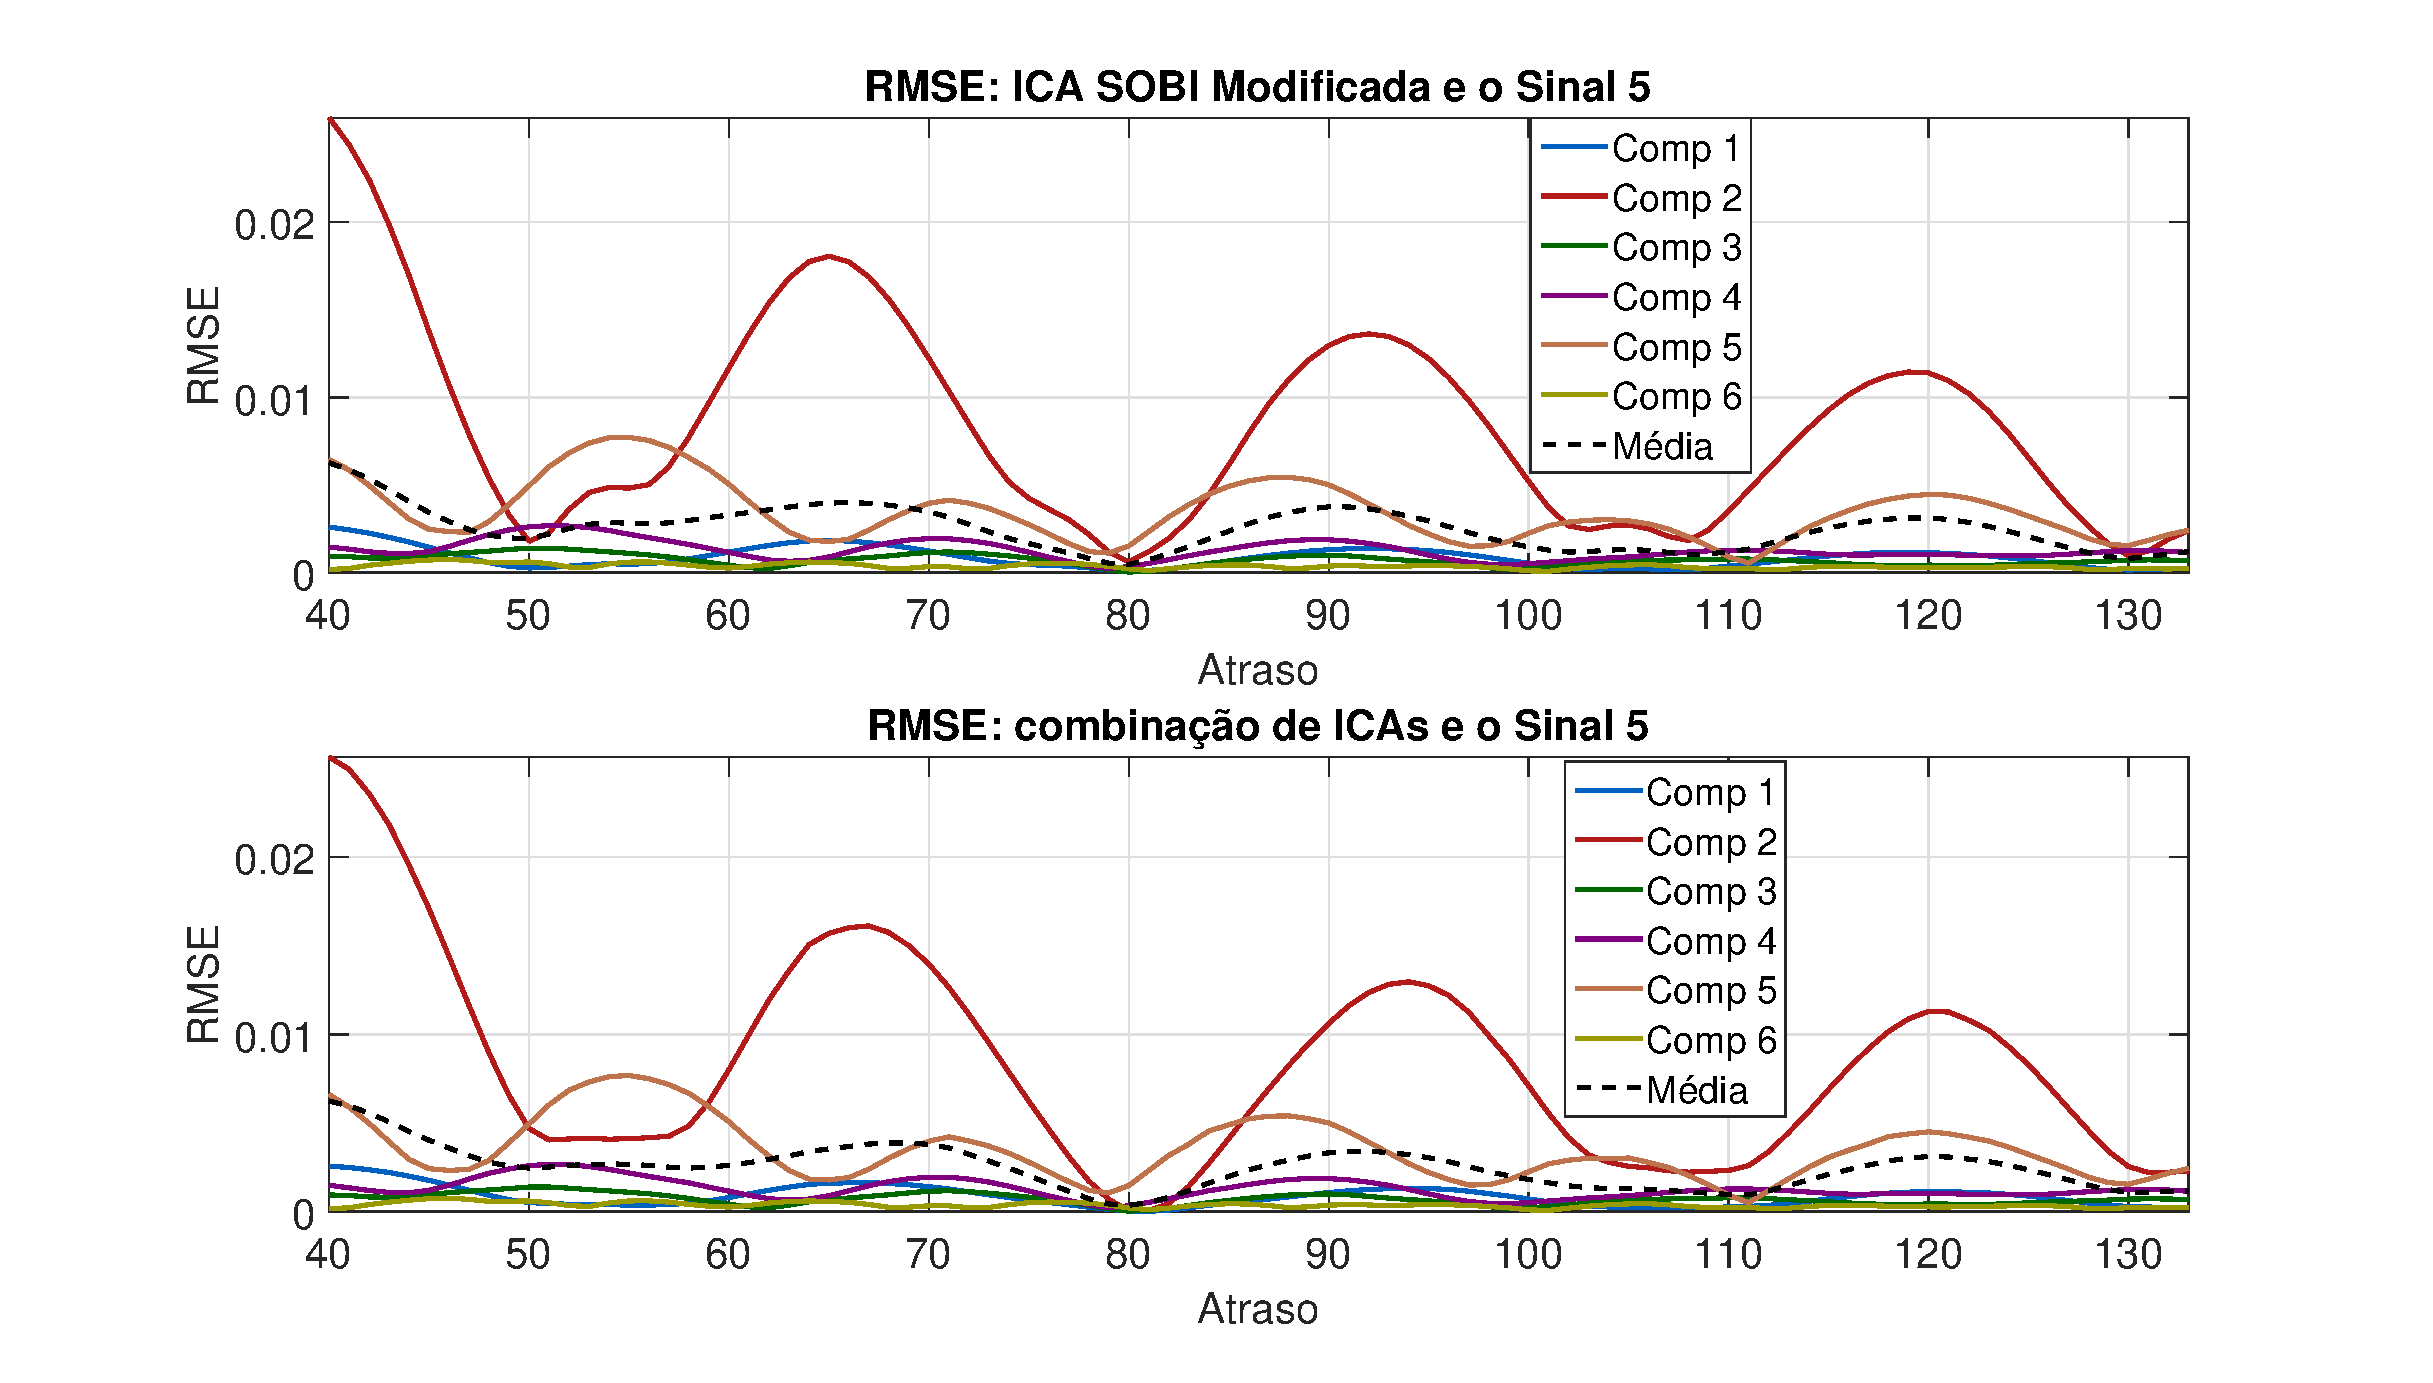
\includegraphics[scale=0.45]{imagens/ImagensParaOAnexo/RMSEcompATodasICAsSinal5.eps}
    \caption{RMSE por componente para as ICAs utilizadas e o S5.}
    \label{fig:RMSEAS5}    
    \end{center}
\end{figure}

\begin{figure}[!htb]
    \begin{center}
    \advance\leftskip -1.5cm
    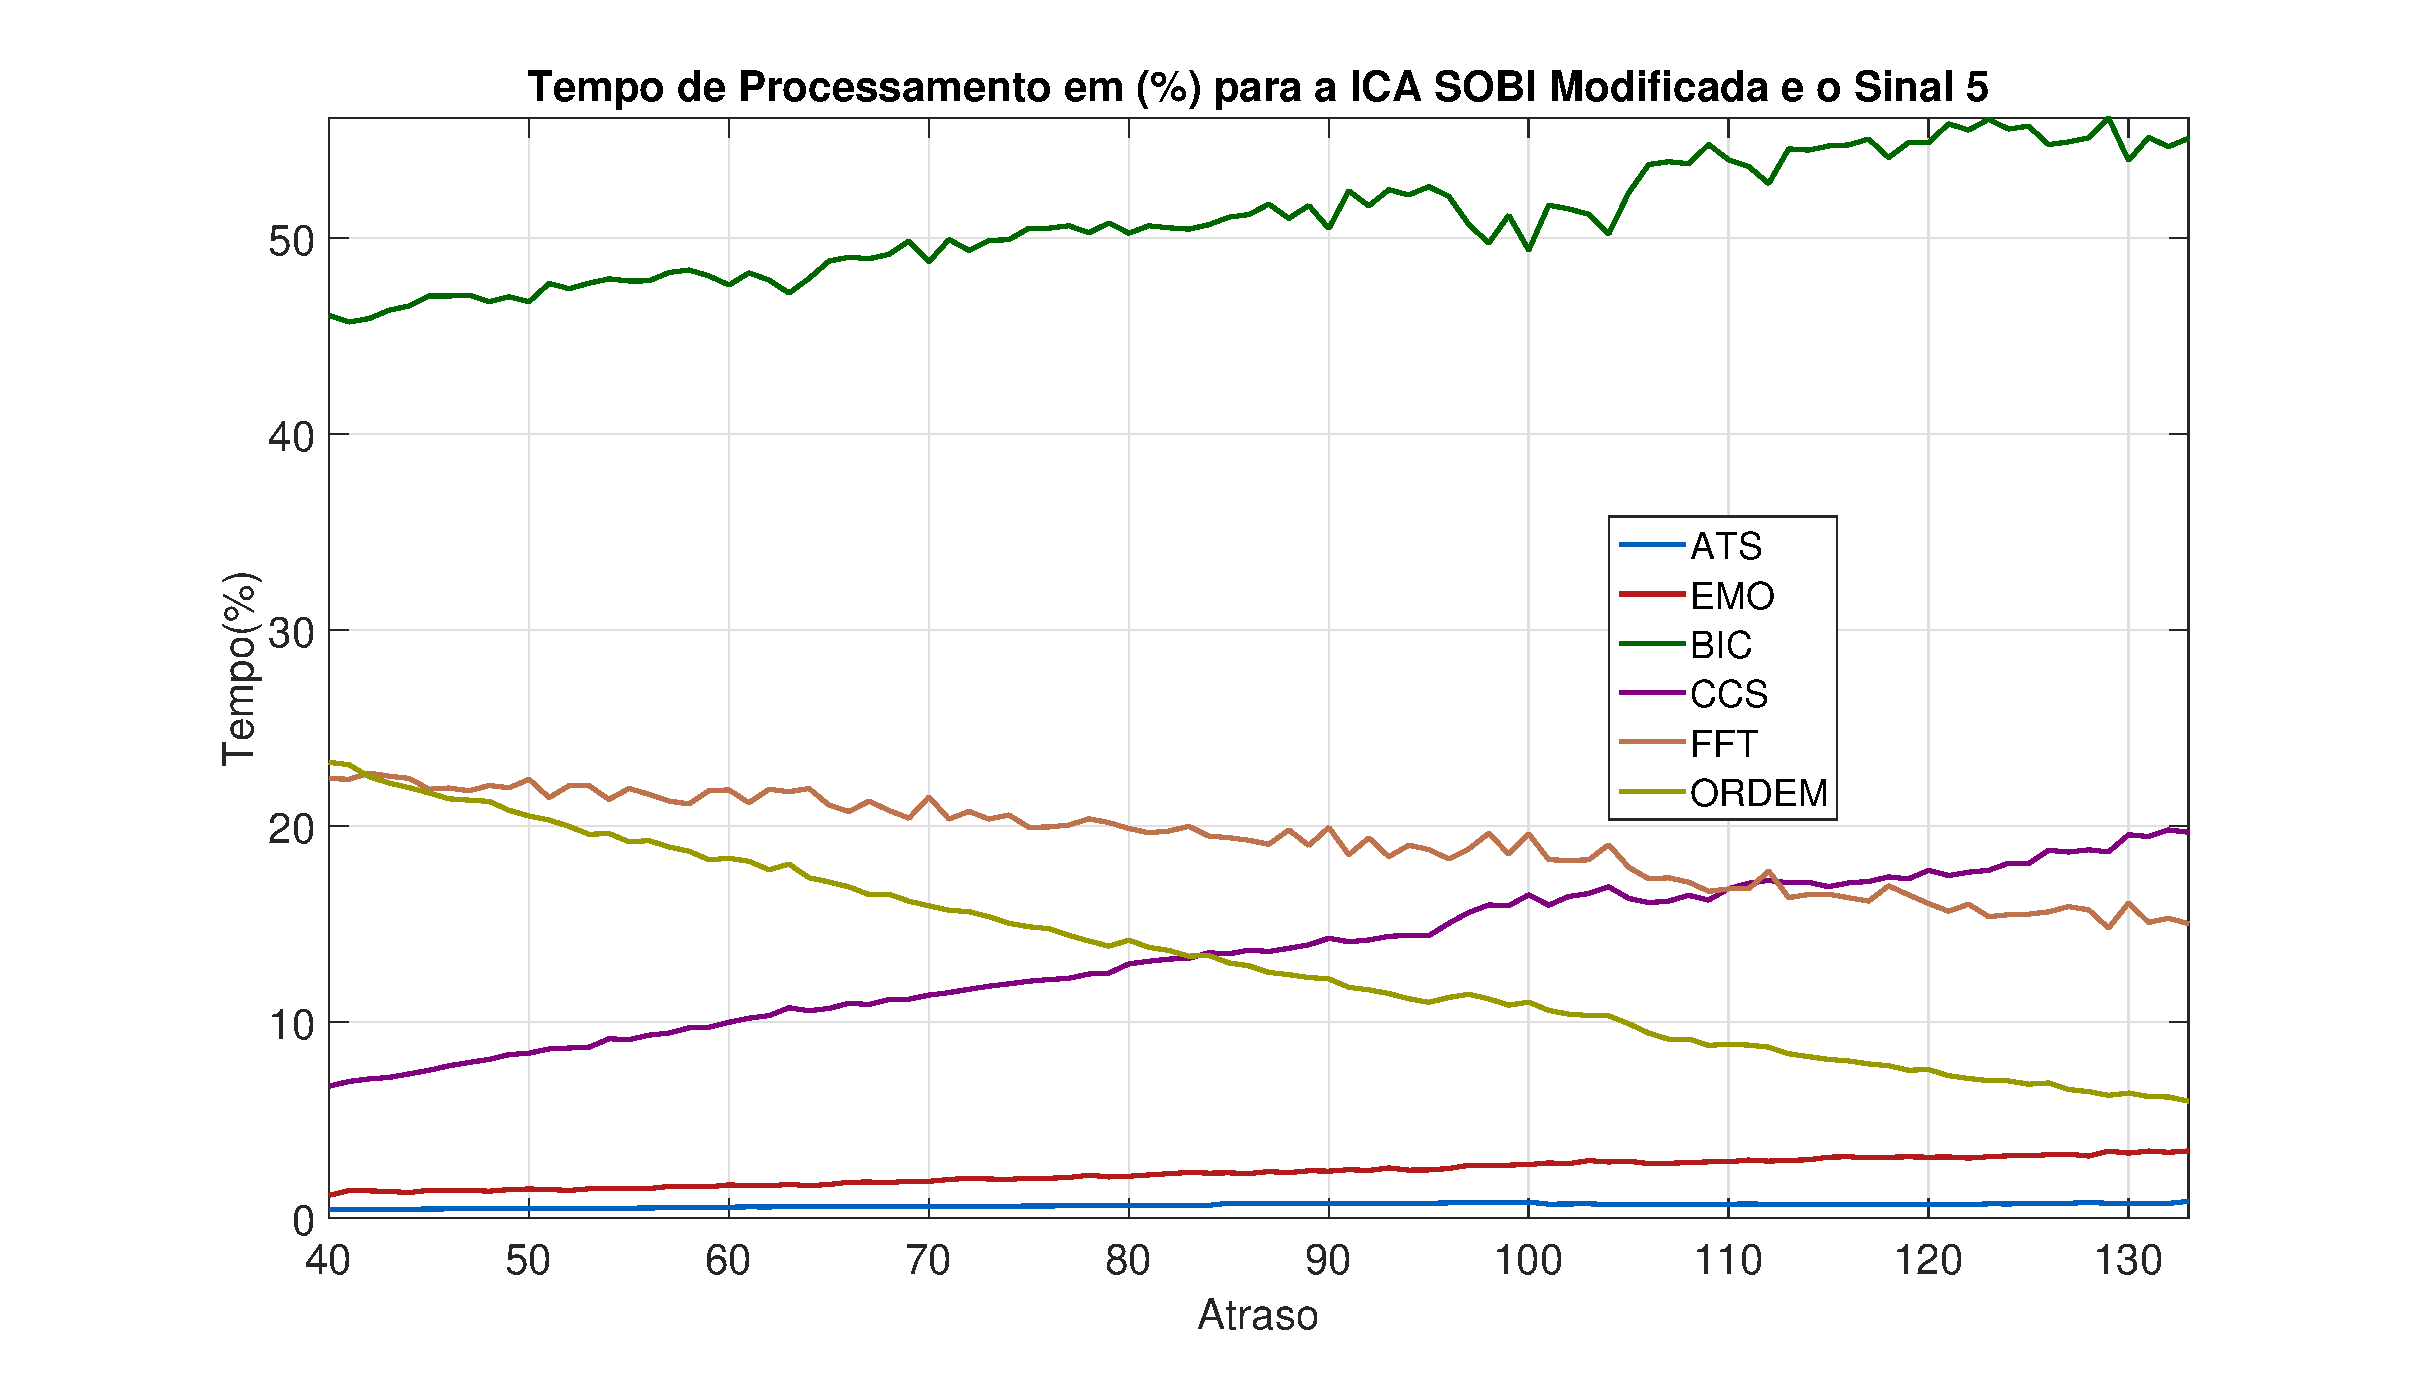
\includegraphics[scale=0.45]{imagens/ImagensParaOAnexo/TPPAICASOBImodSinal5.eps}
    \caption{TP em porcentagem dos testes para ICA SOBI modificado em S5.}
    \label{fig:TPSMAS5}    
    \end{center}
\end{figure}

\begin{figure}[!htb]
    \begin{center}
    \advance\leftskip -1.5cm
    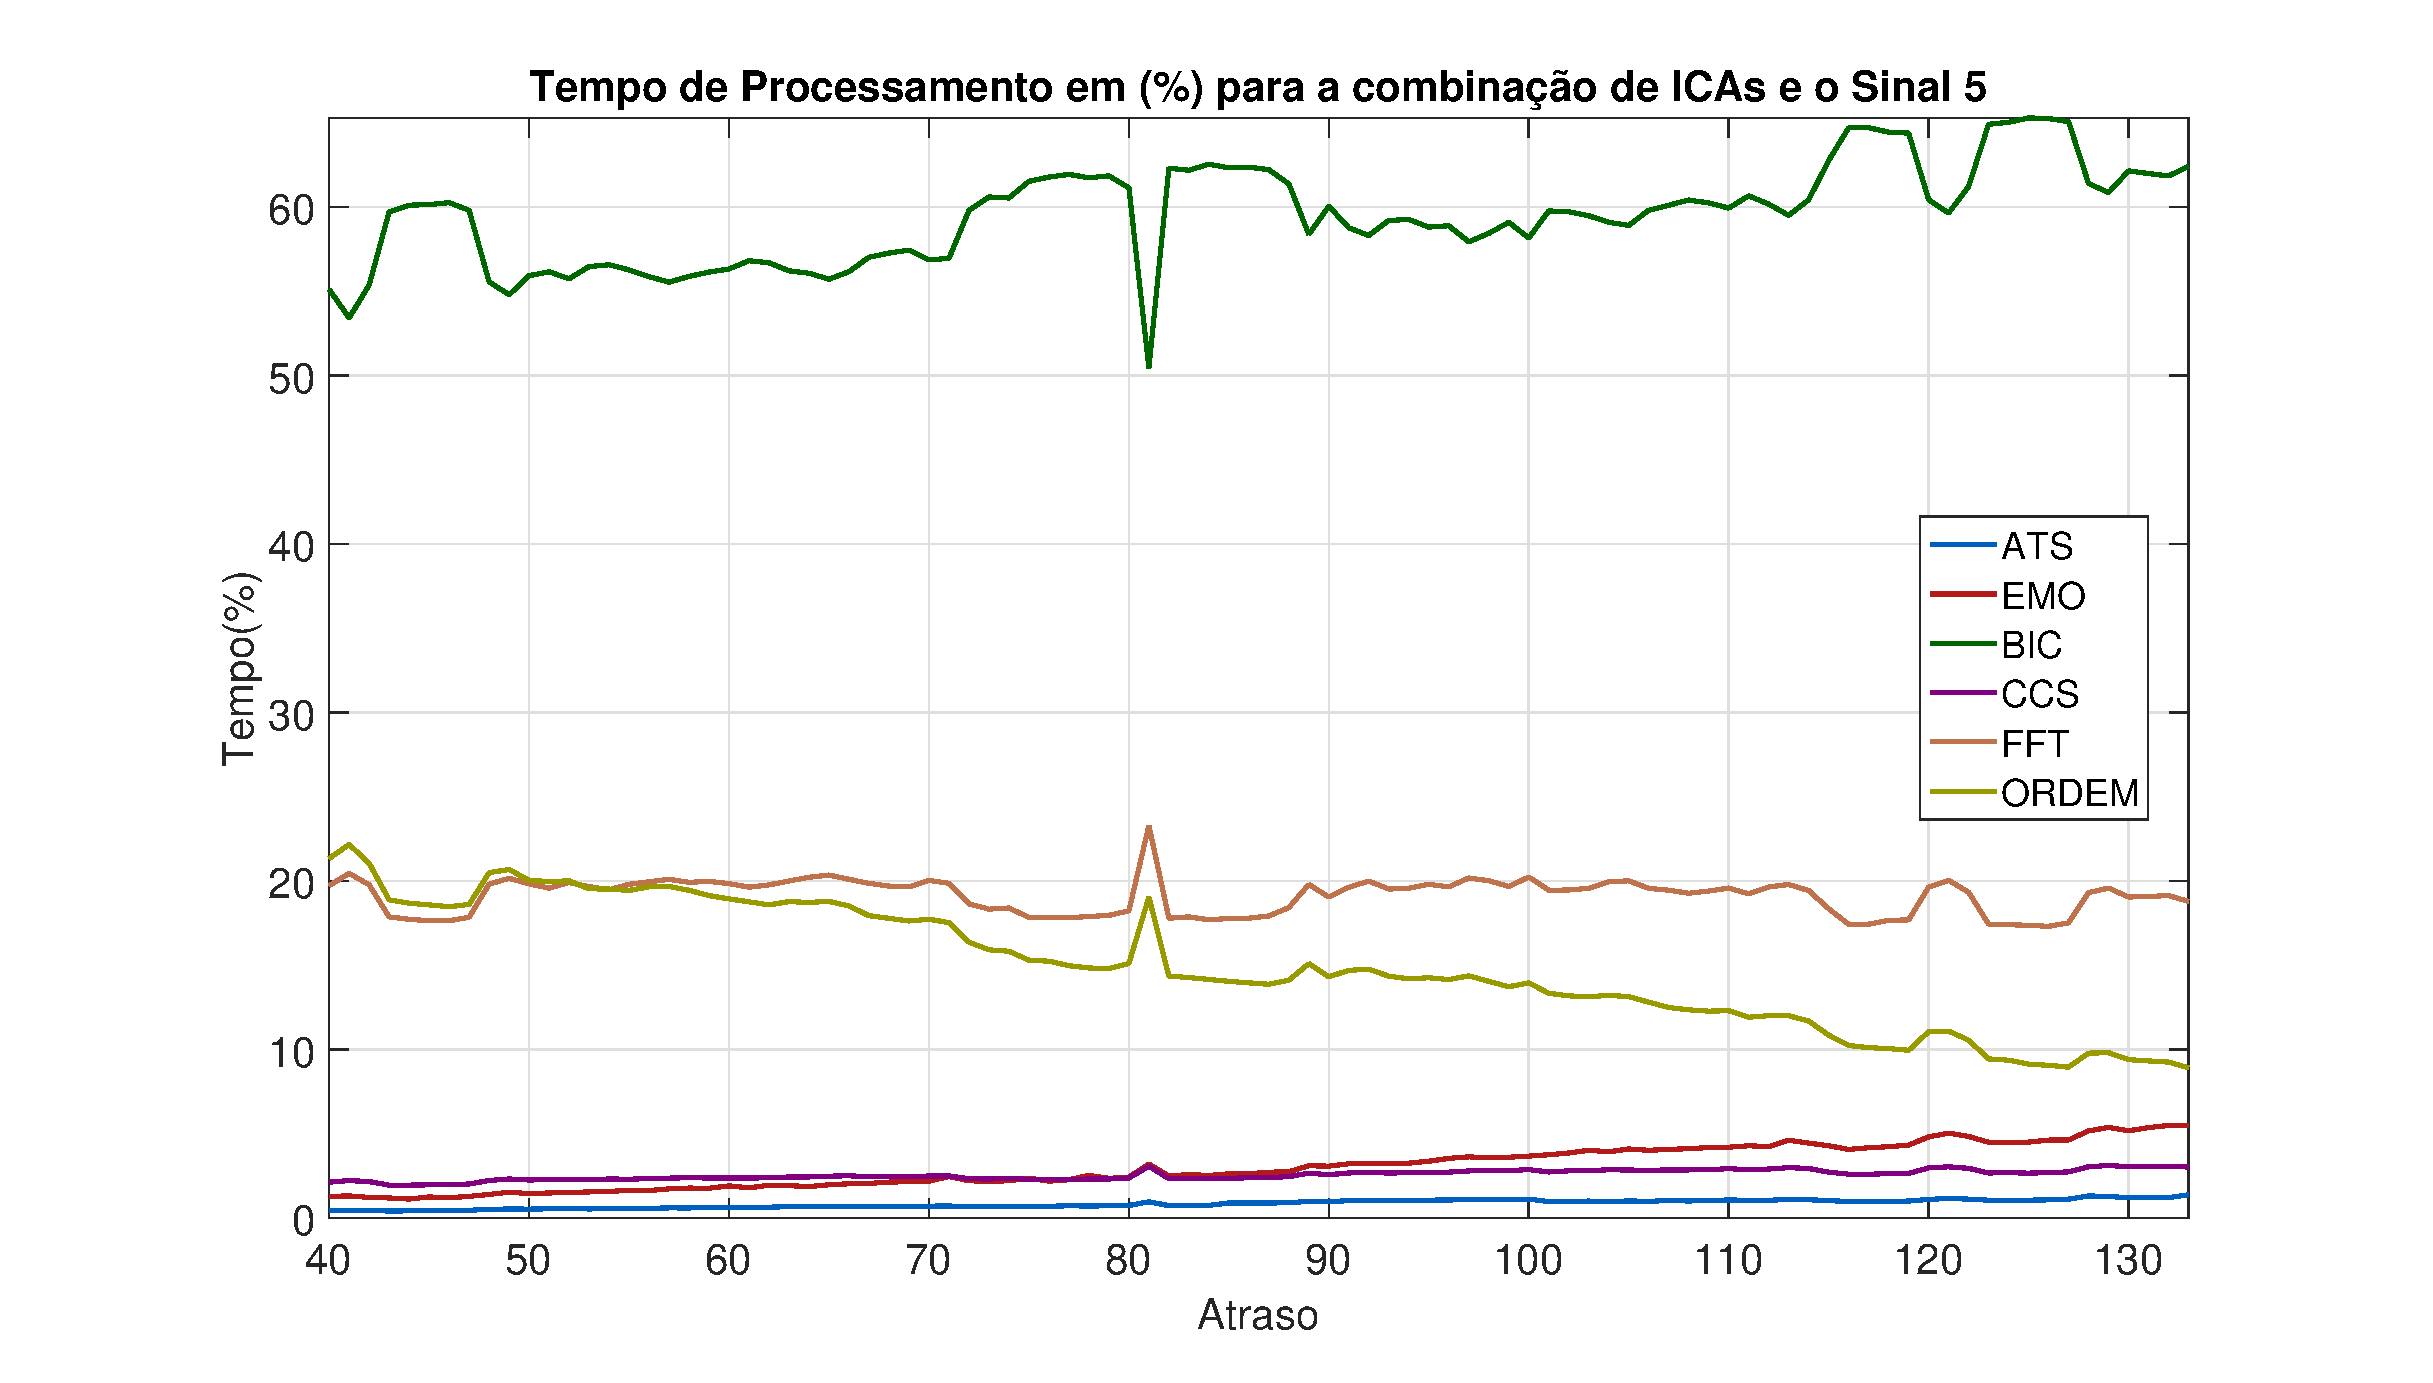
\includegraphics[scale=0.45]{imagens/ImagensParaOAnexo/TPPACombinacaoICASinal5.eps}
    \caption{TP em porcentagem dos testes para combinação de ICAs em S5.}
    \label{fig:TPCIAS5}    
    \end{center}
\end{figure}

\begin{figure}[!htb]
    \begin{center}
    \advance\leftskip -1.5cm
    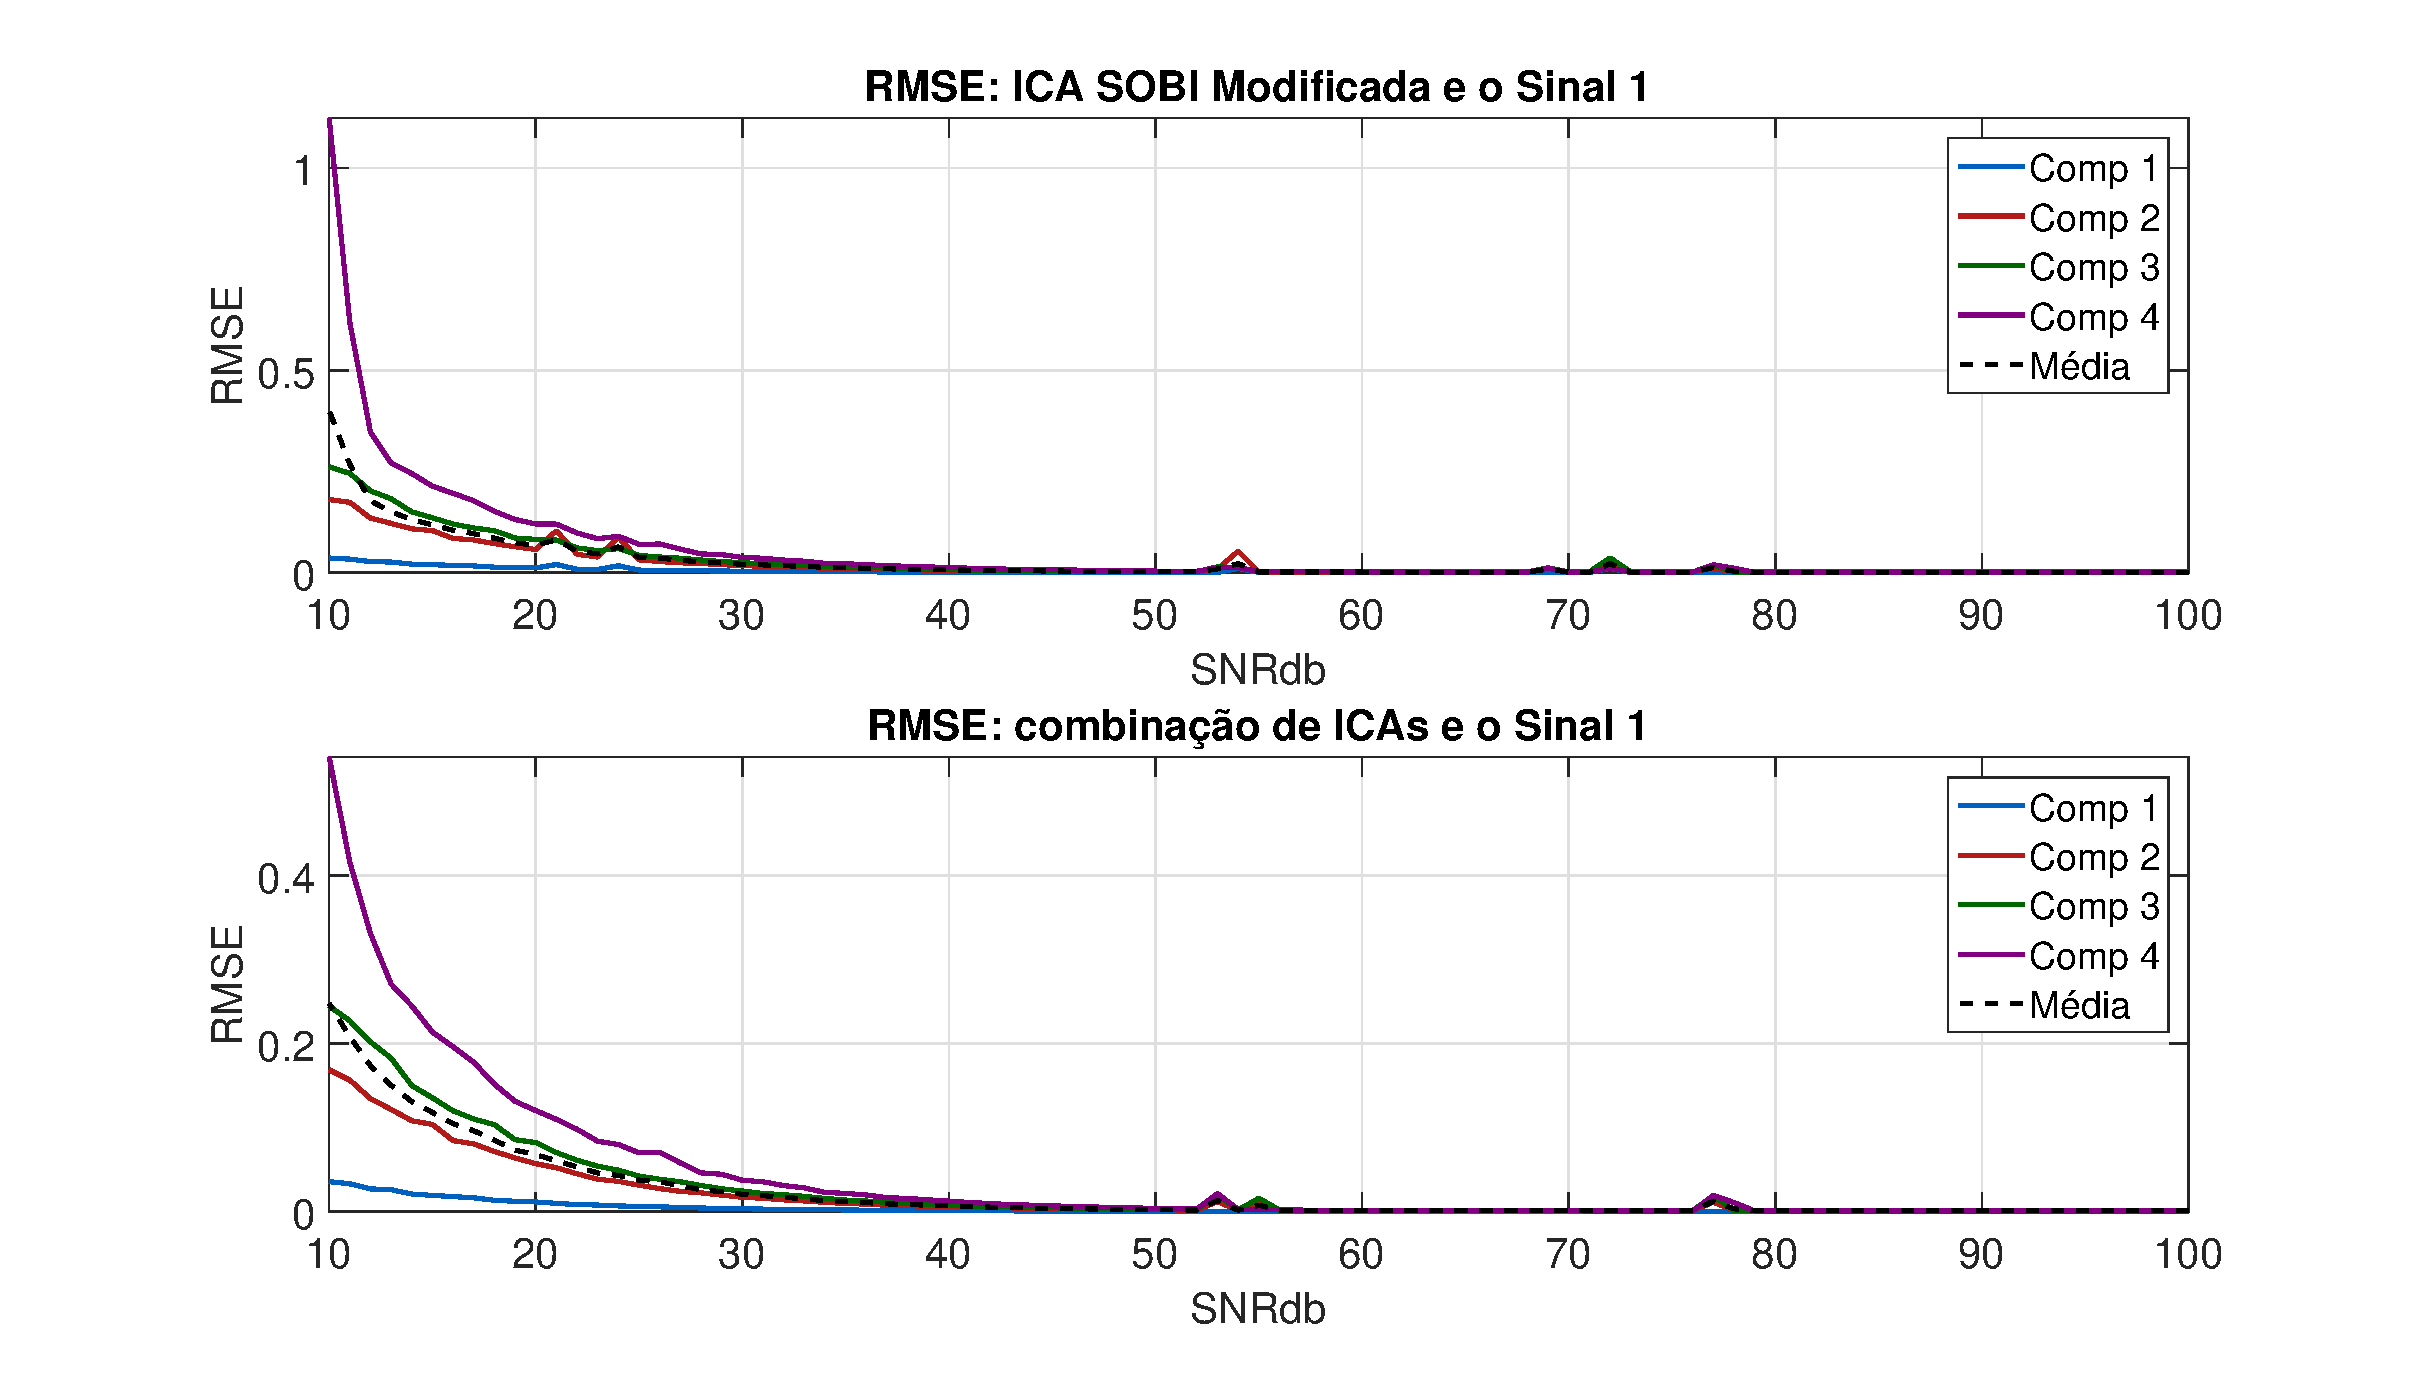
\includegraphics[scale=0.45]{imagens/ImagensParaOAnexo/RMSEcompRTodasICAsSinal1.eps}
    \caption{RMSE por componente para as ICAs utilizadas na variação de ruido e o S1.}
    \label{fig:RMSERS1}    
    \end{center}
\end{figure}

\begin{figure}[!htb]
    \begin{center}
    \advance\leftskip -1.5cm
    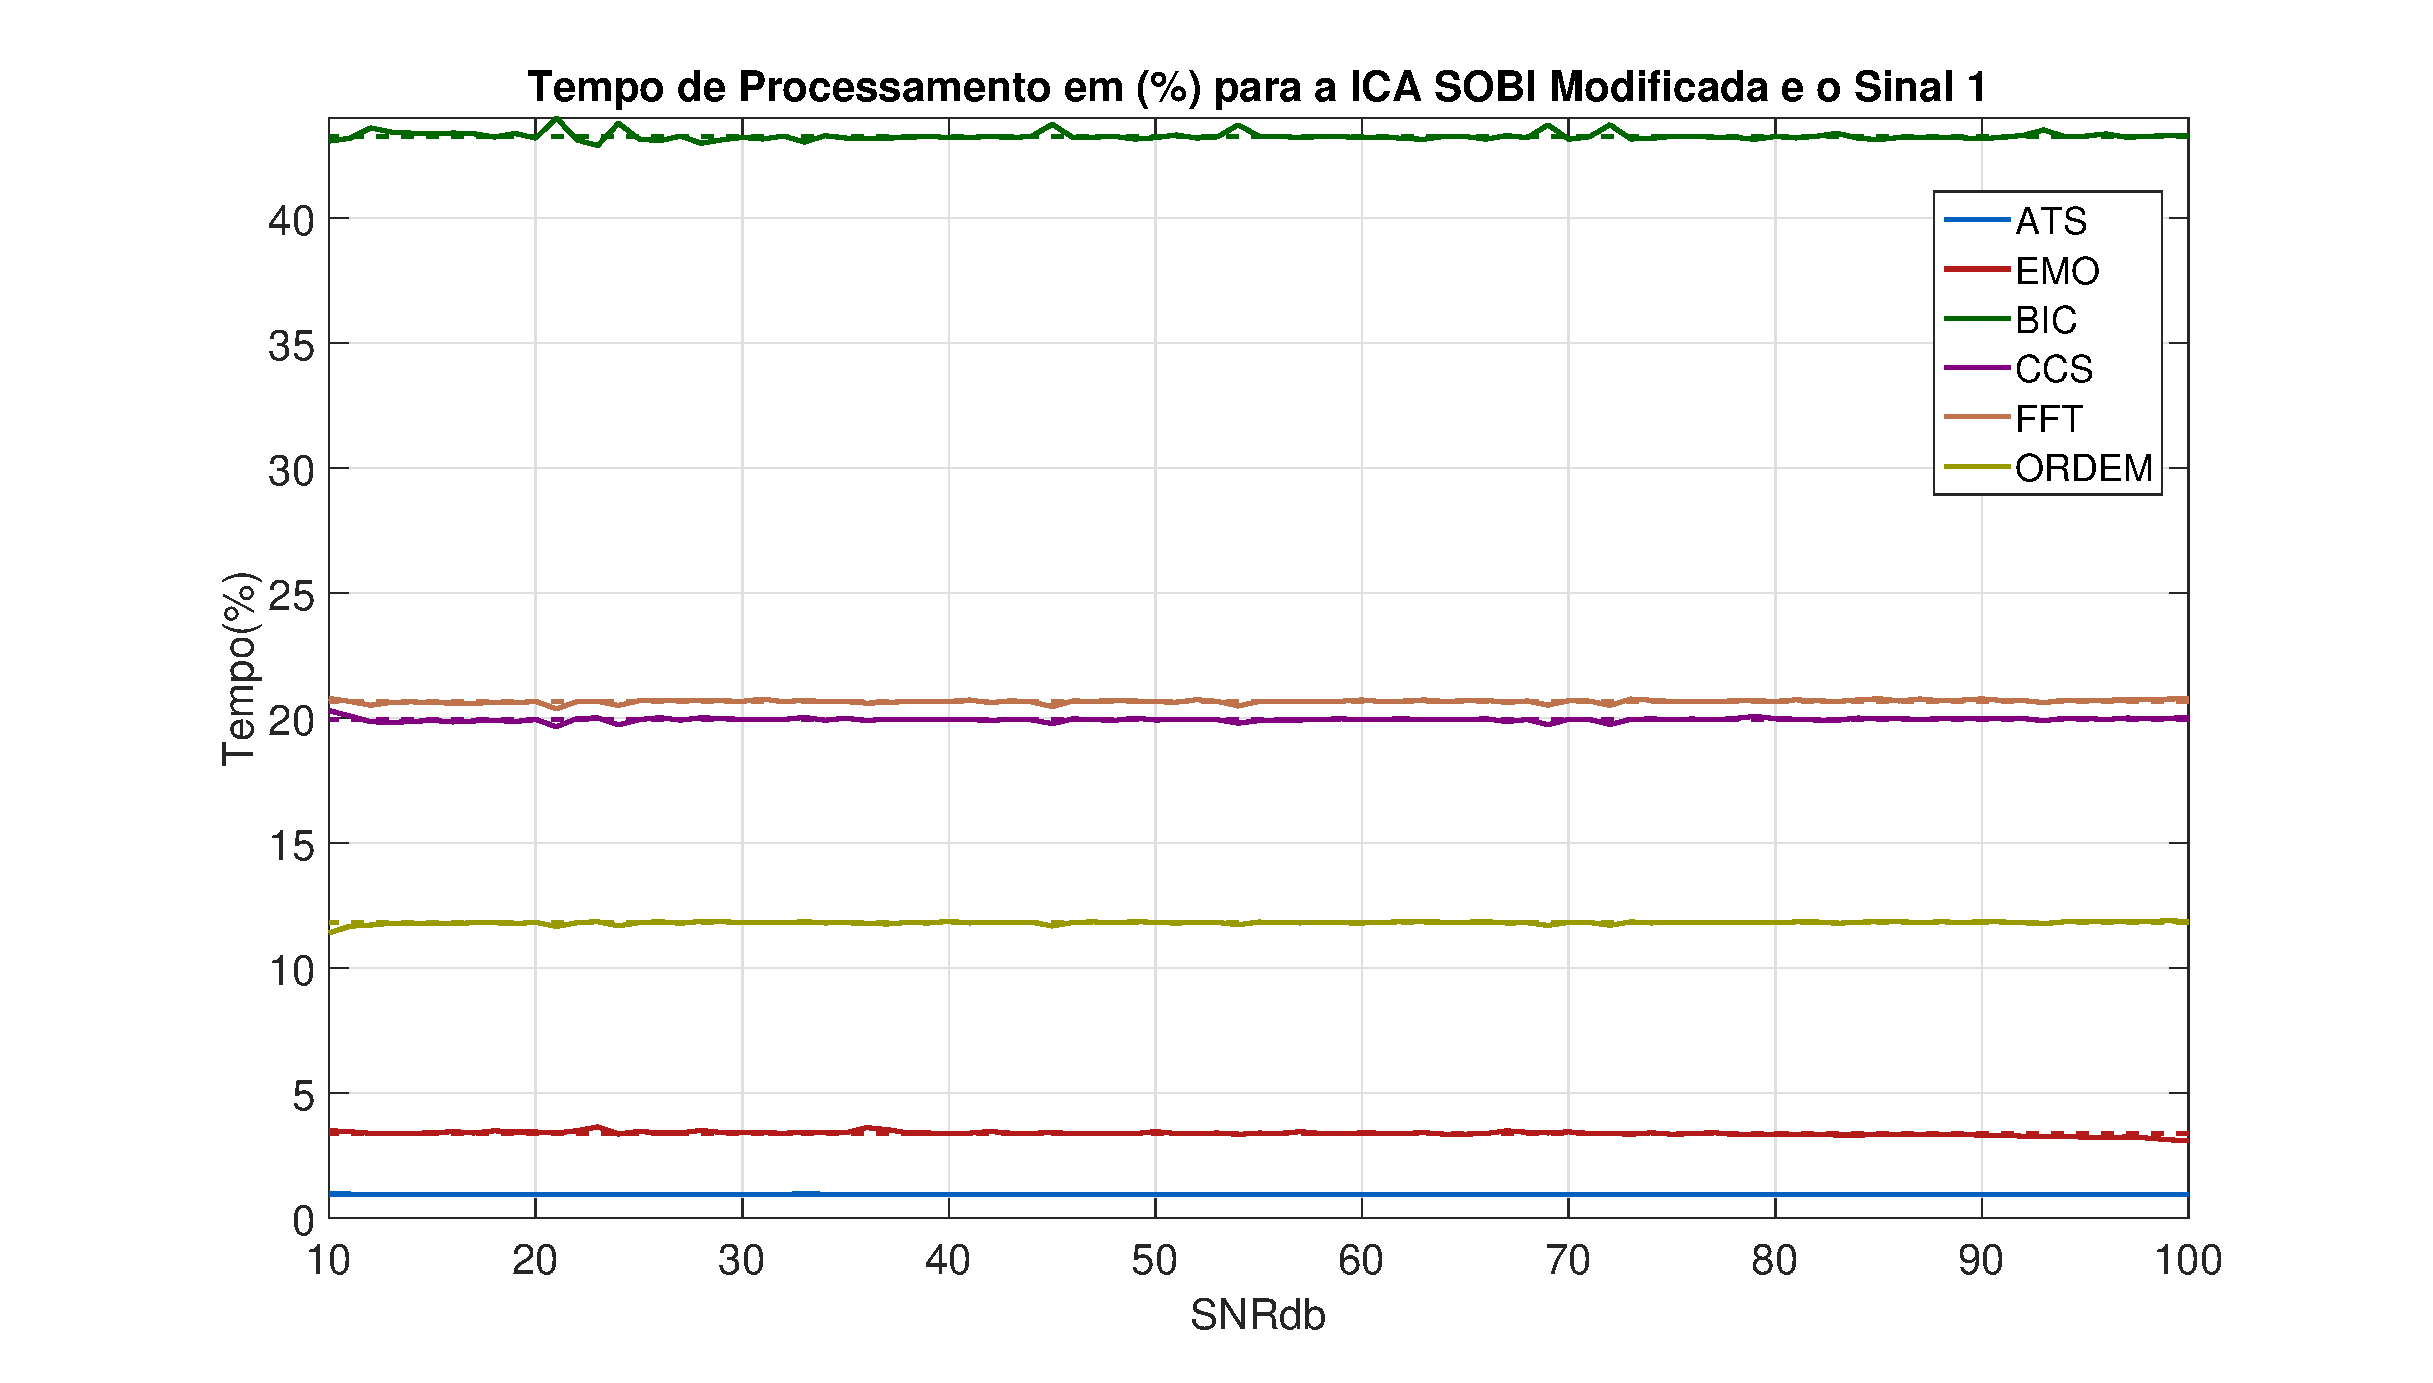
\includegraphics[scale=0.45]{imagens/ImagensParaOAnexo/TPPRICASOBImodSinal1.eps}
    \caption{TP em porcentagem dos testes para ICA SOBI modificado em S1.}
    \label{fig:TPSMRS1}    
    \end{center}
\end{figure}

\begin{figure}[!htb]
    \begin{center}
    \advance\leftskip -1.5cm
    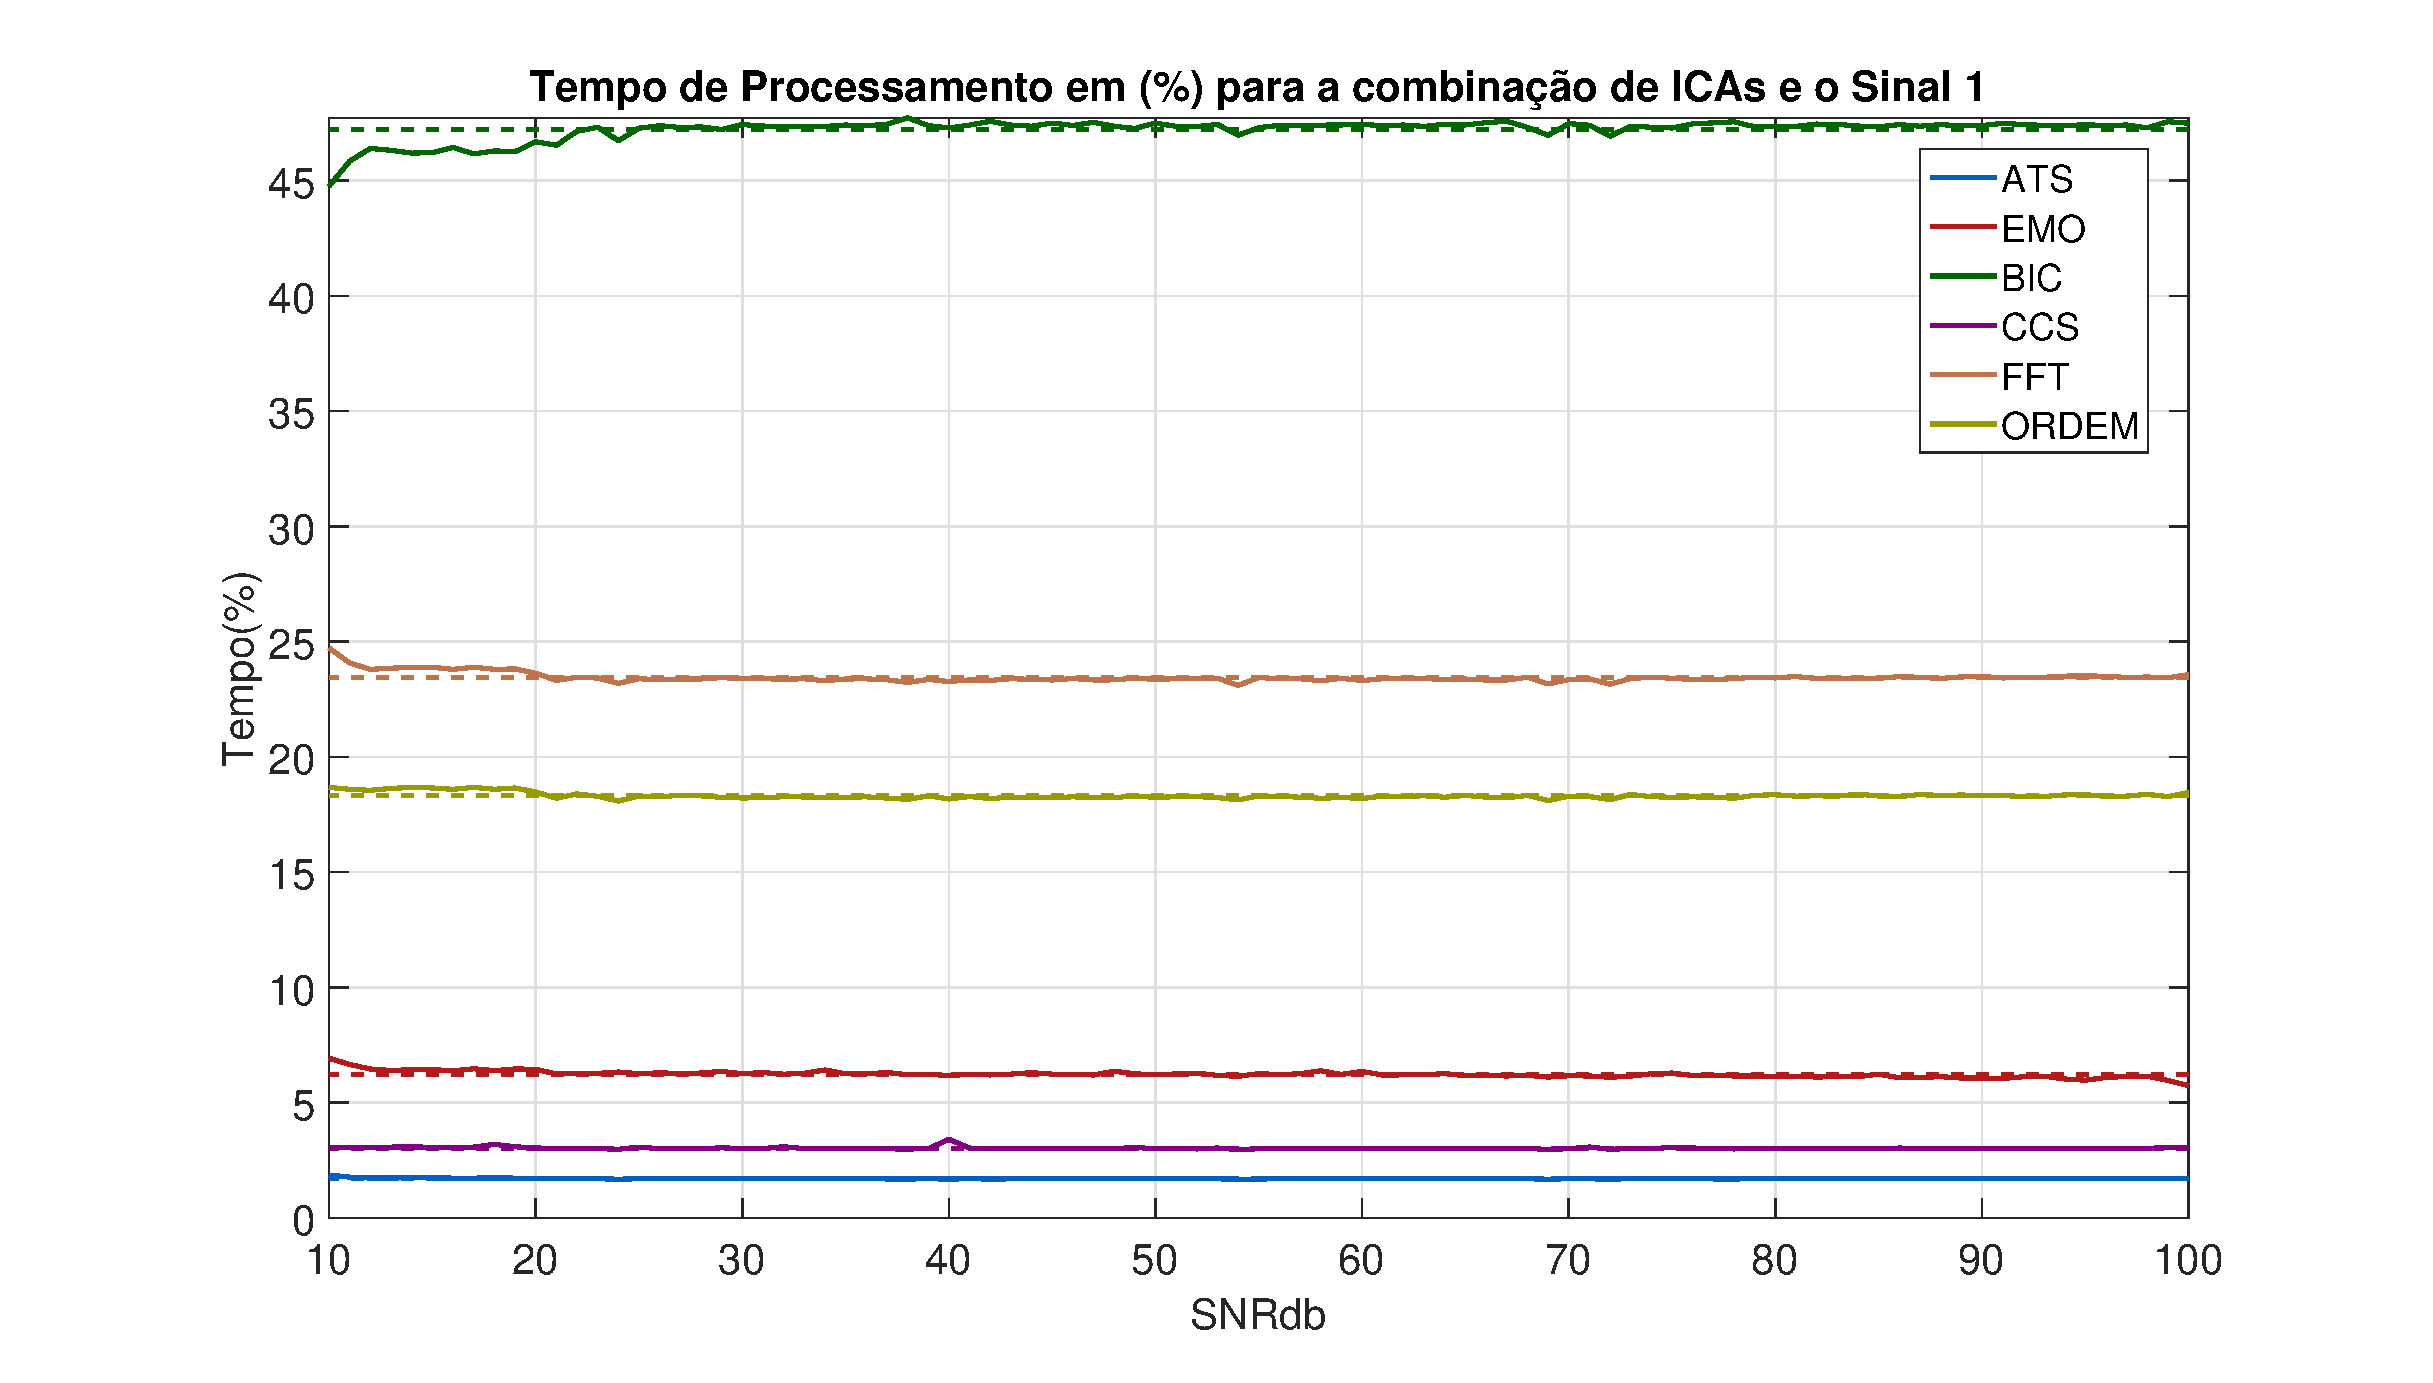
\includegraphics[scale=0.45]{imagens/ImagensParaOAnexo/TPPRCombinacaoICASinal1.eps}
    \caption{TP em porcentagem dos testes para combinação de ICAs em S1.}
    \label{fig:TPCIRS1}    
    \end{center}
\end{figure}

\begin{figure}[!htb]
    \begin{center}
    \advance\leftskip -1.5cm
    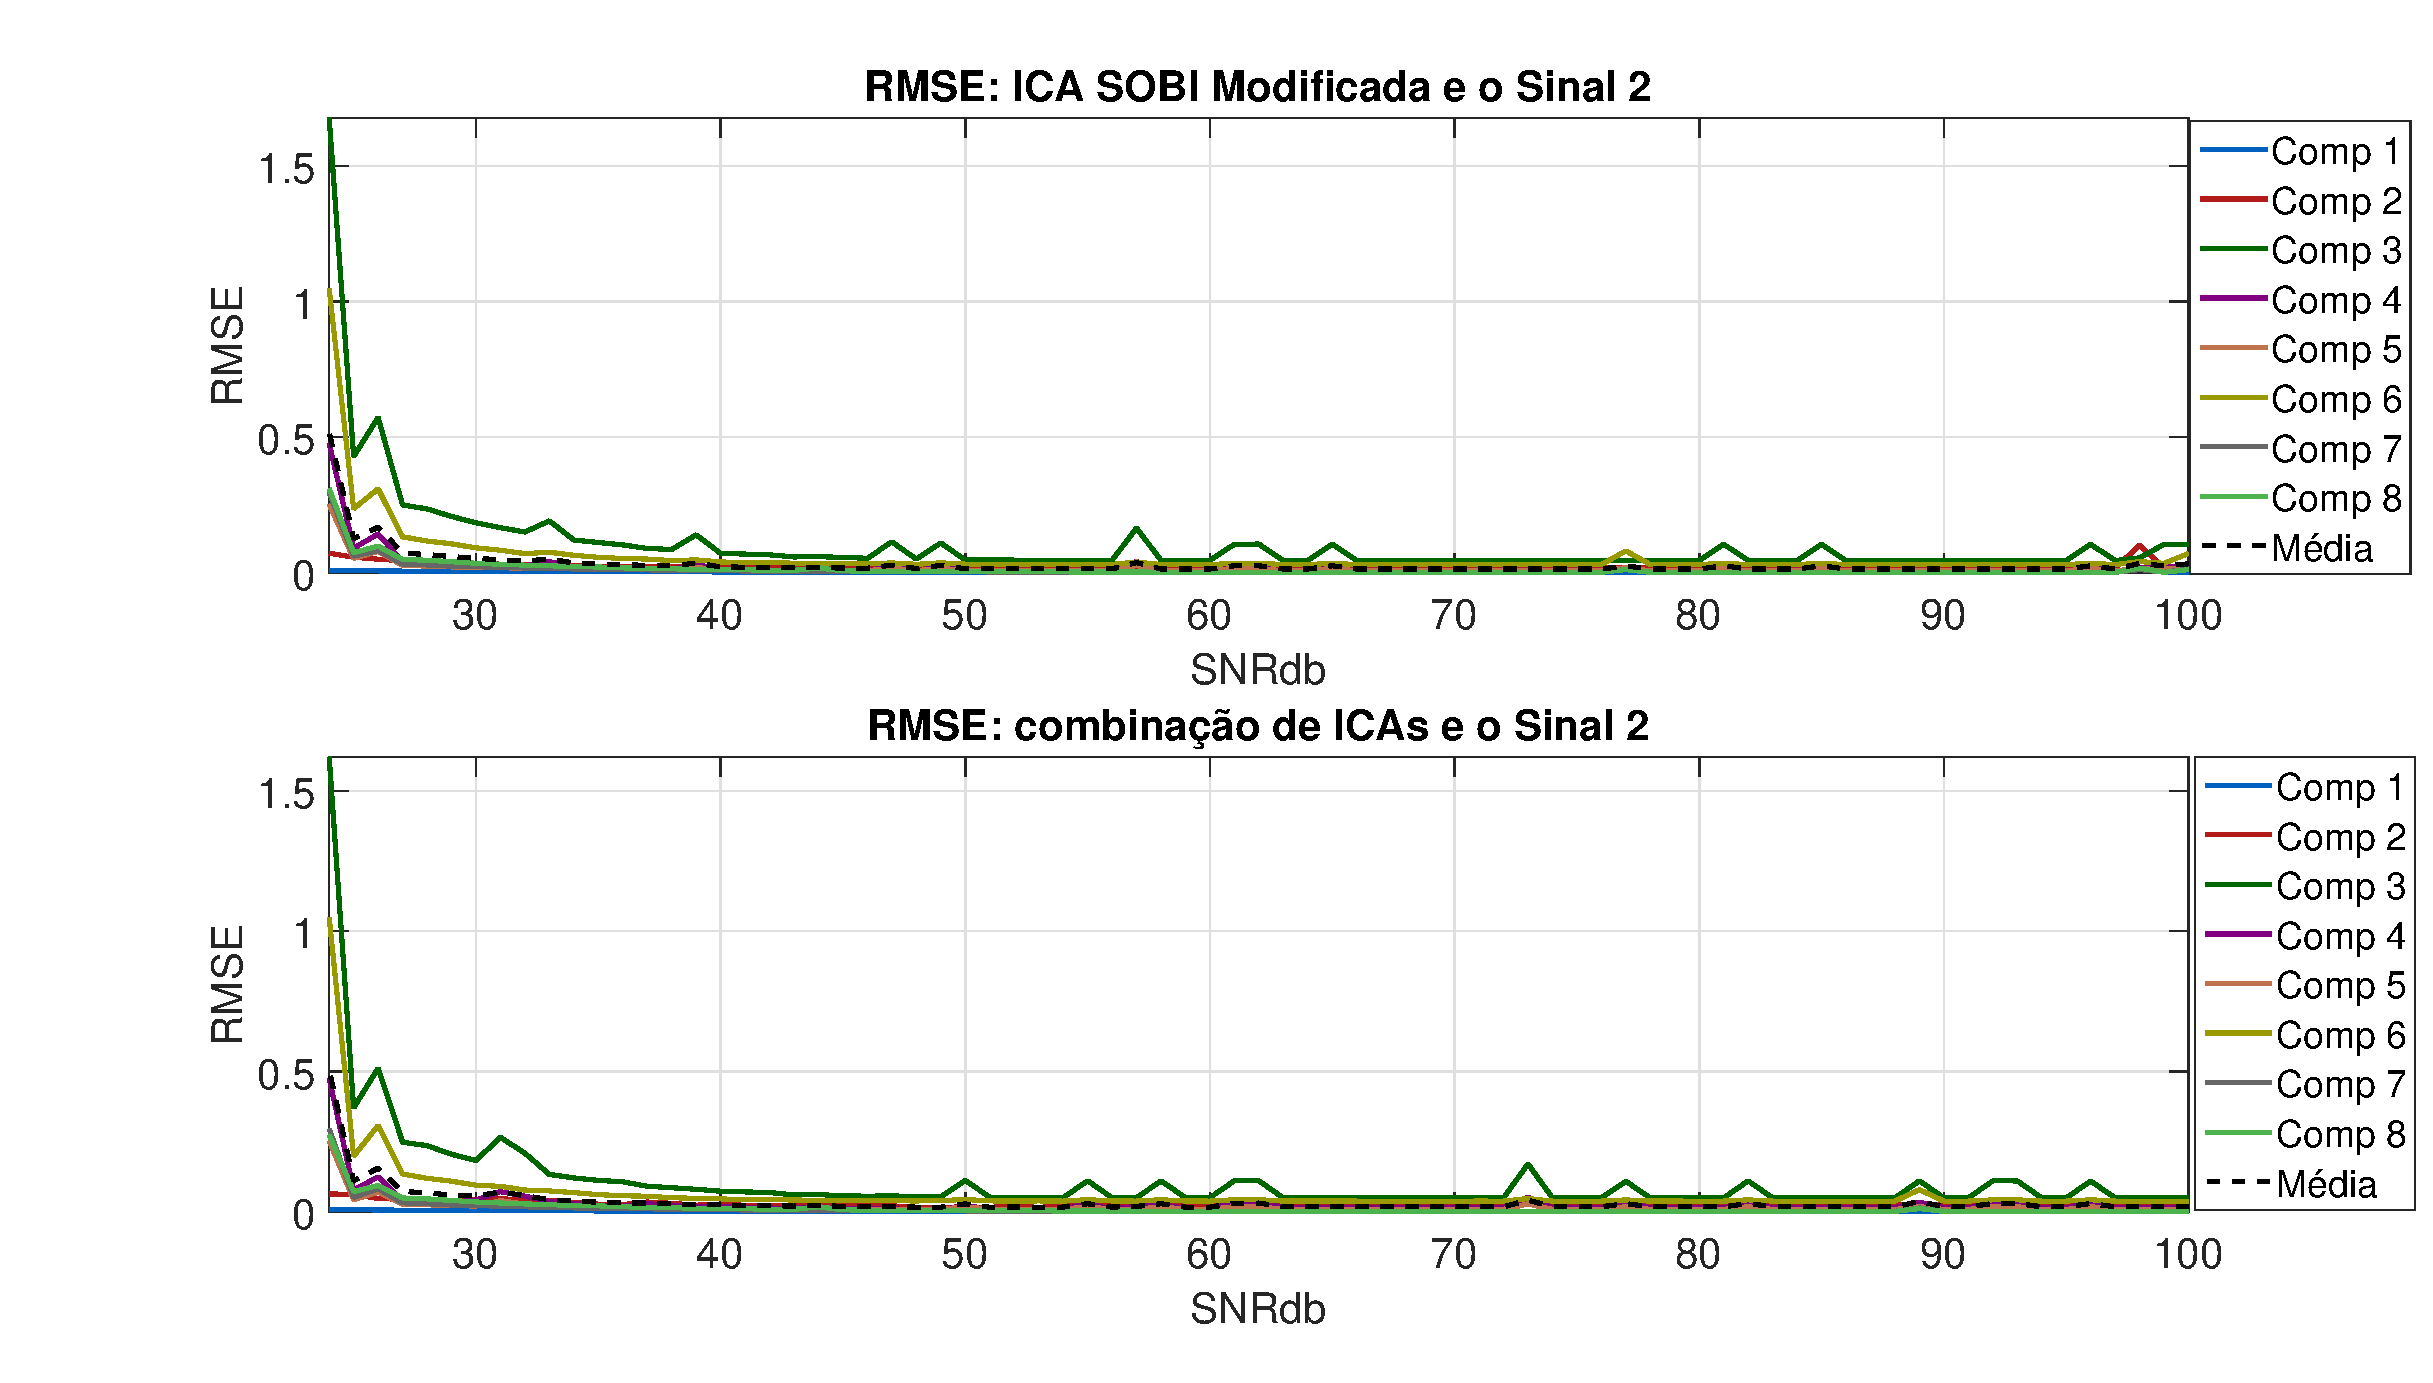
\includegraphics[scale=0.45]{imagens/ImagensParaOAnexo/RMSEcompRTodasICAsSinal2.eps}
    \caption{RMSE por componente para as ICAs utilizadas na variação de ruido e o S2.}
    \label{fig:RMSERS2}    
    \end{center}
\end{figure}

\begin{figure}[!htb]
    \begin{center}
    \advance\leftskip -1.5cm
    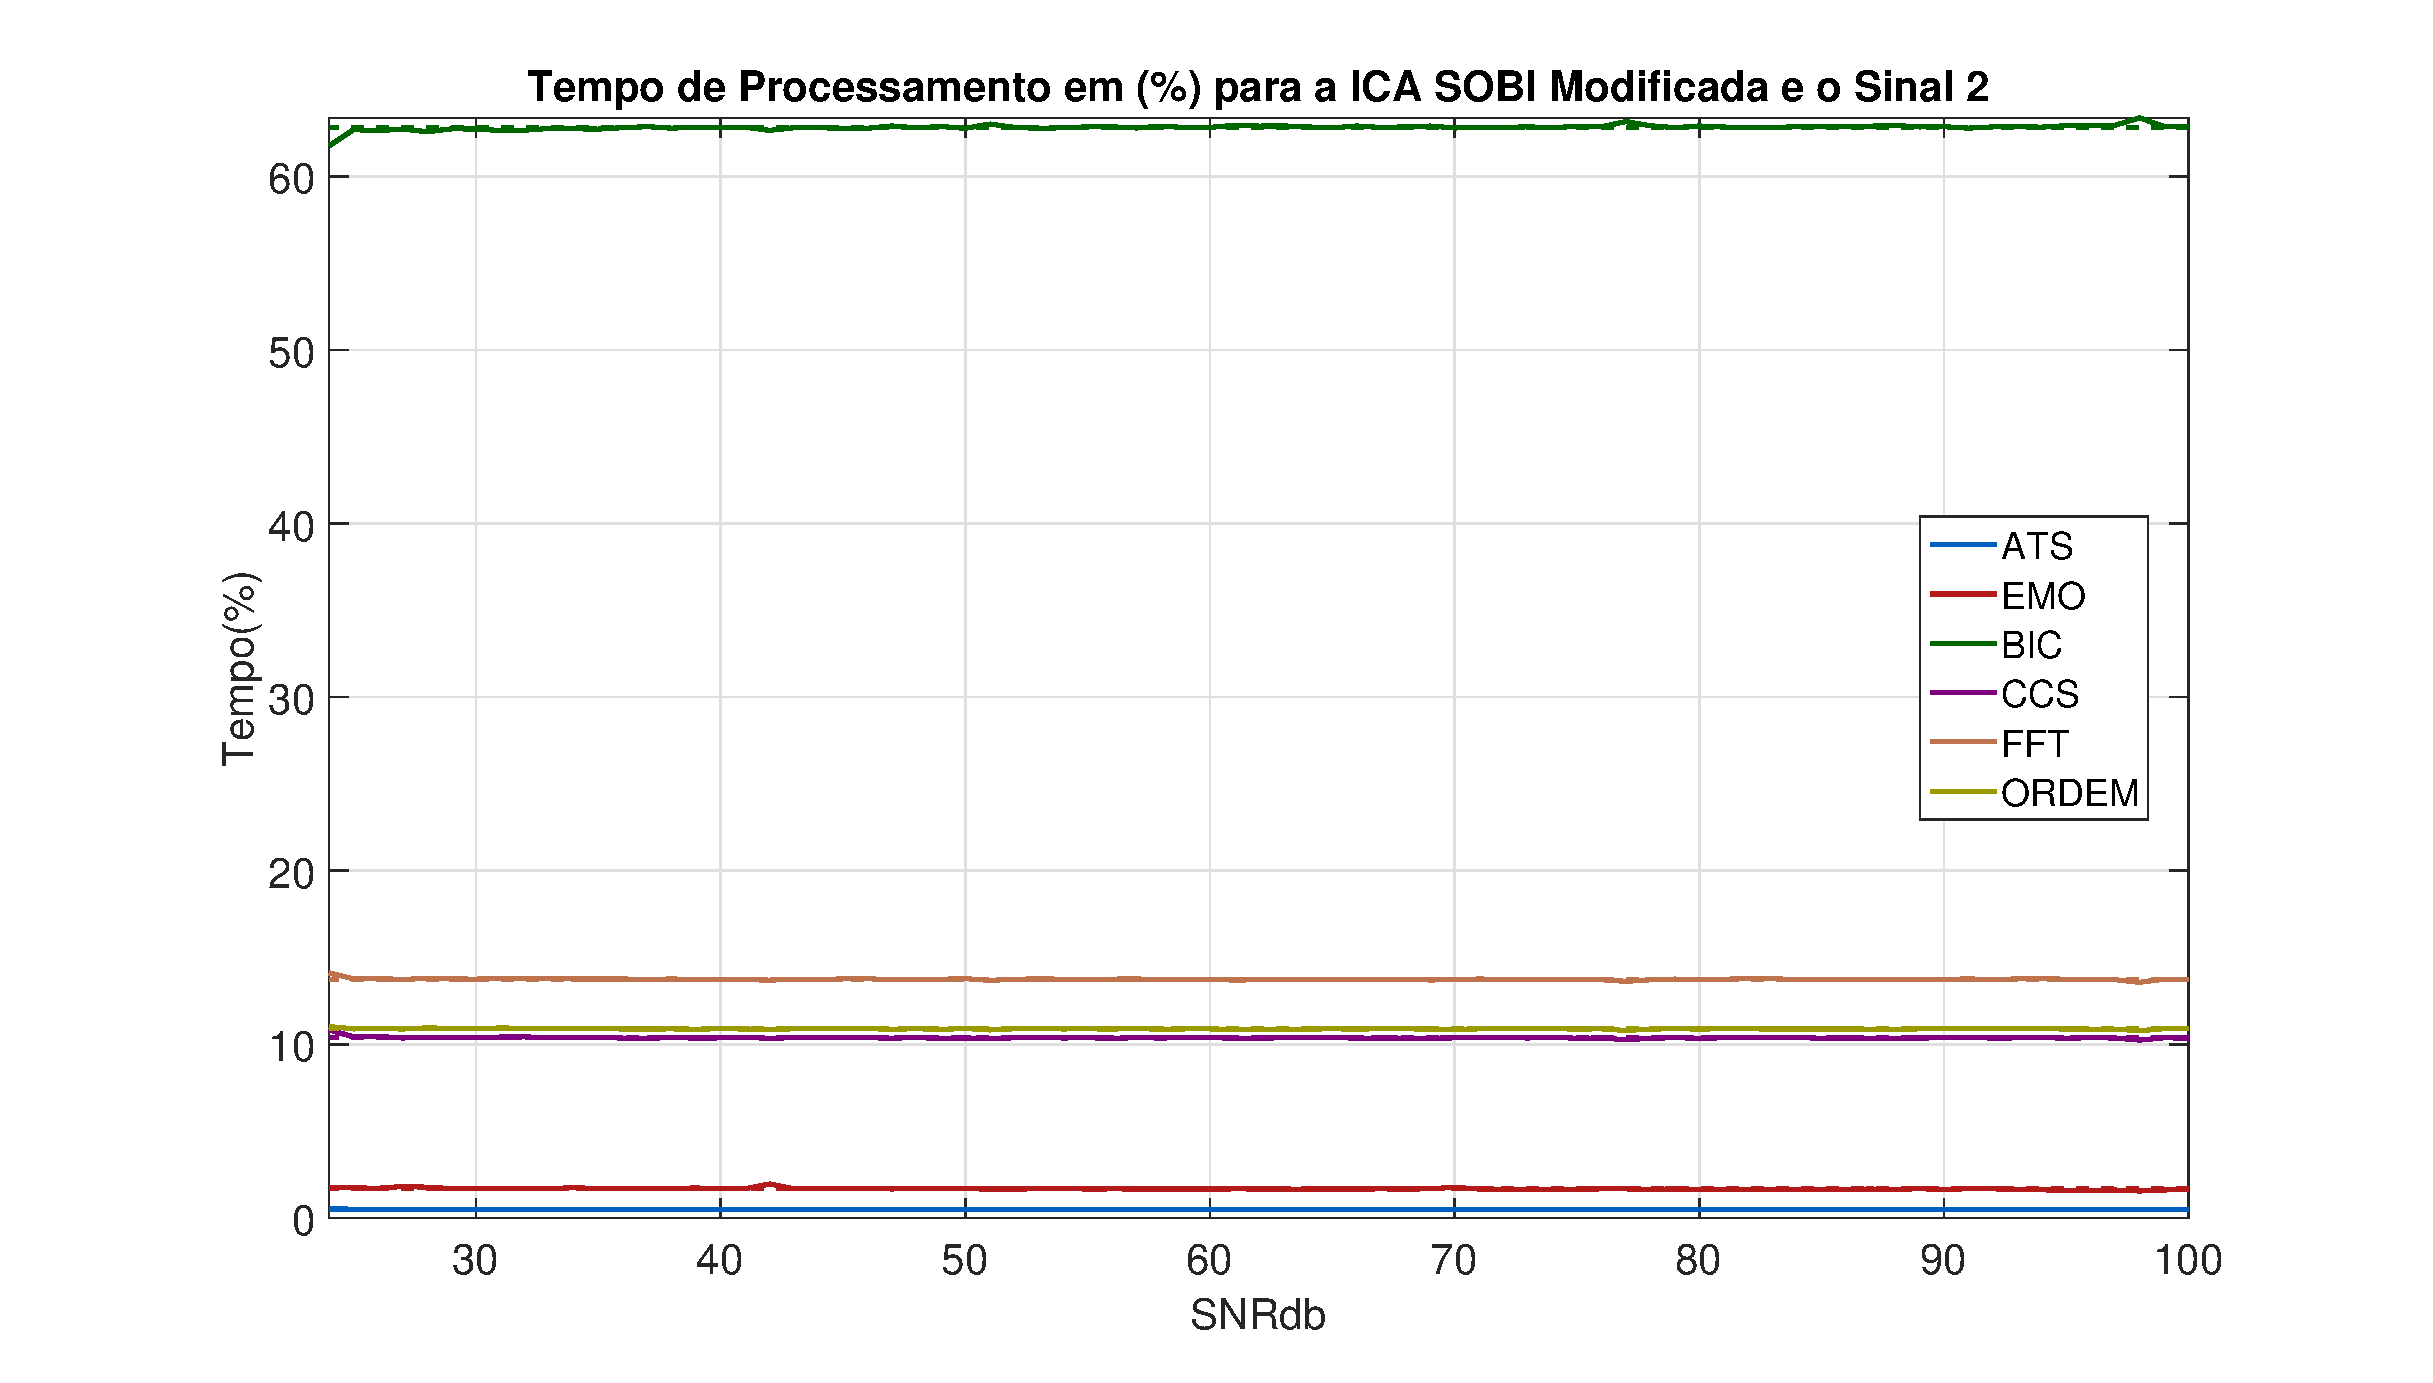
\includegraphics[scale=0.45]{imagens/ImagensParaOAnexo/TPPRICASOBImodSinal2.eps}
    \caption{TP em porcentagem dos testes para ICA SOBI modificado em S2.}
    \label{fig:TPSMRS2}    
    \end{center}
\end{figure}

\begin{figure}[!htb]
    \begin{center}
    \advance\leftskip -1.5cm
    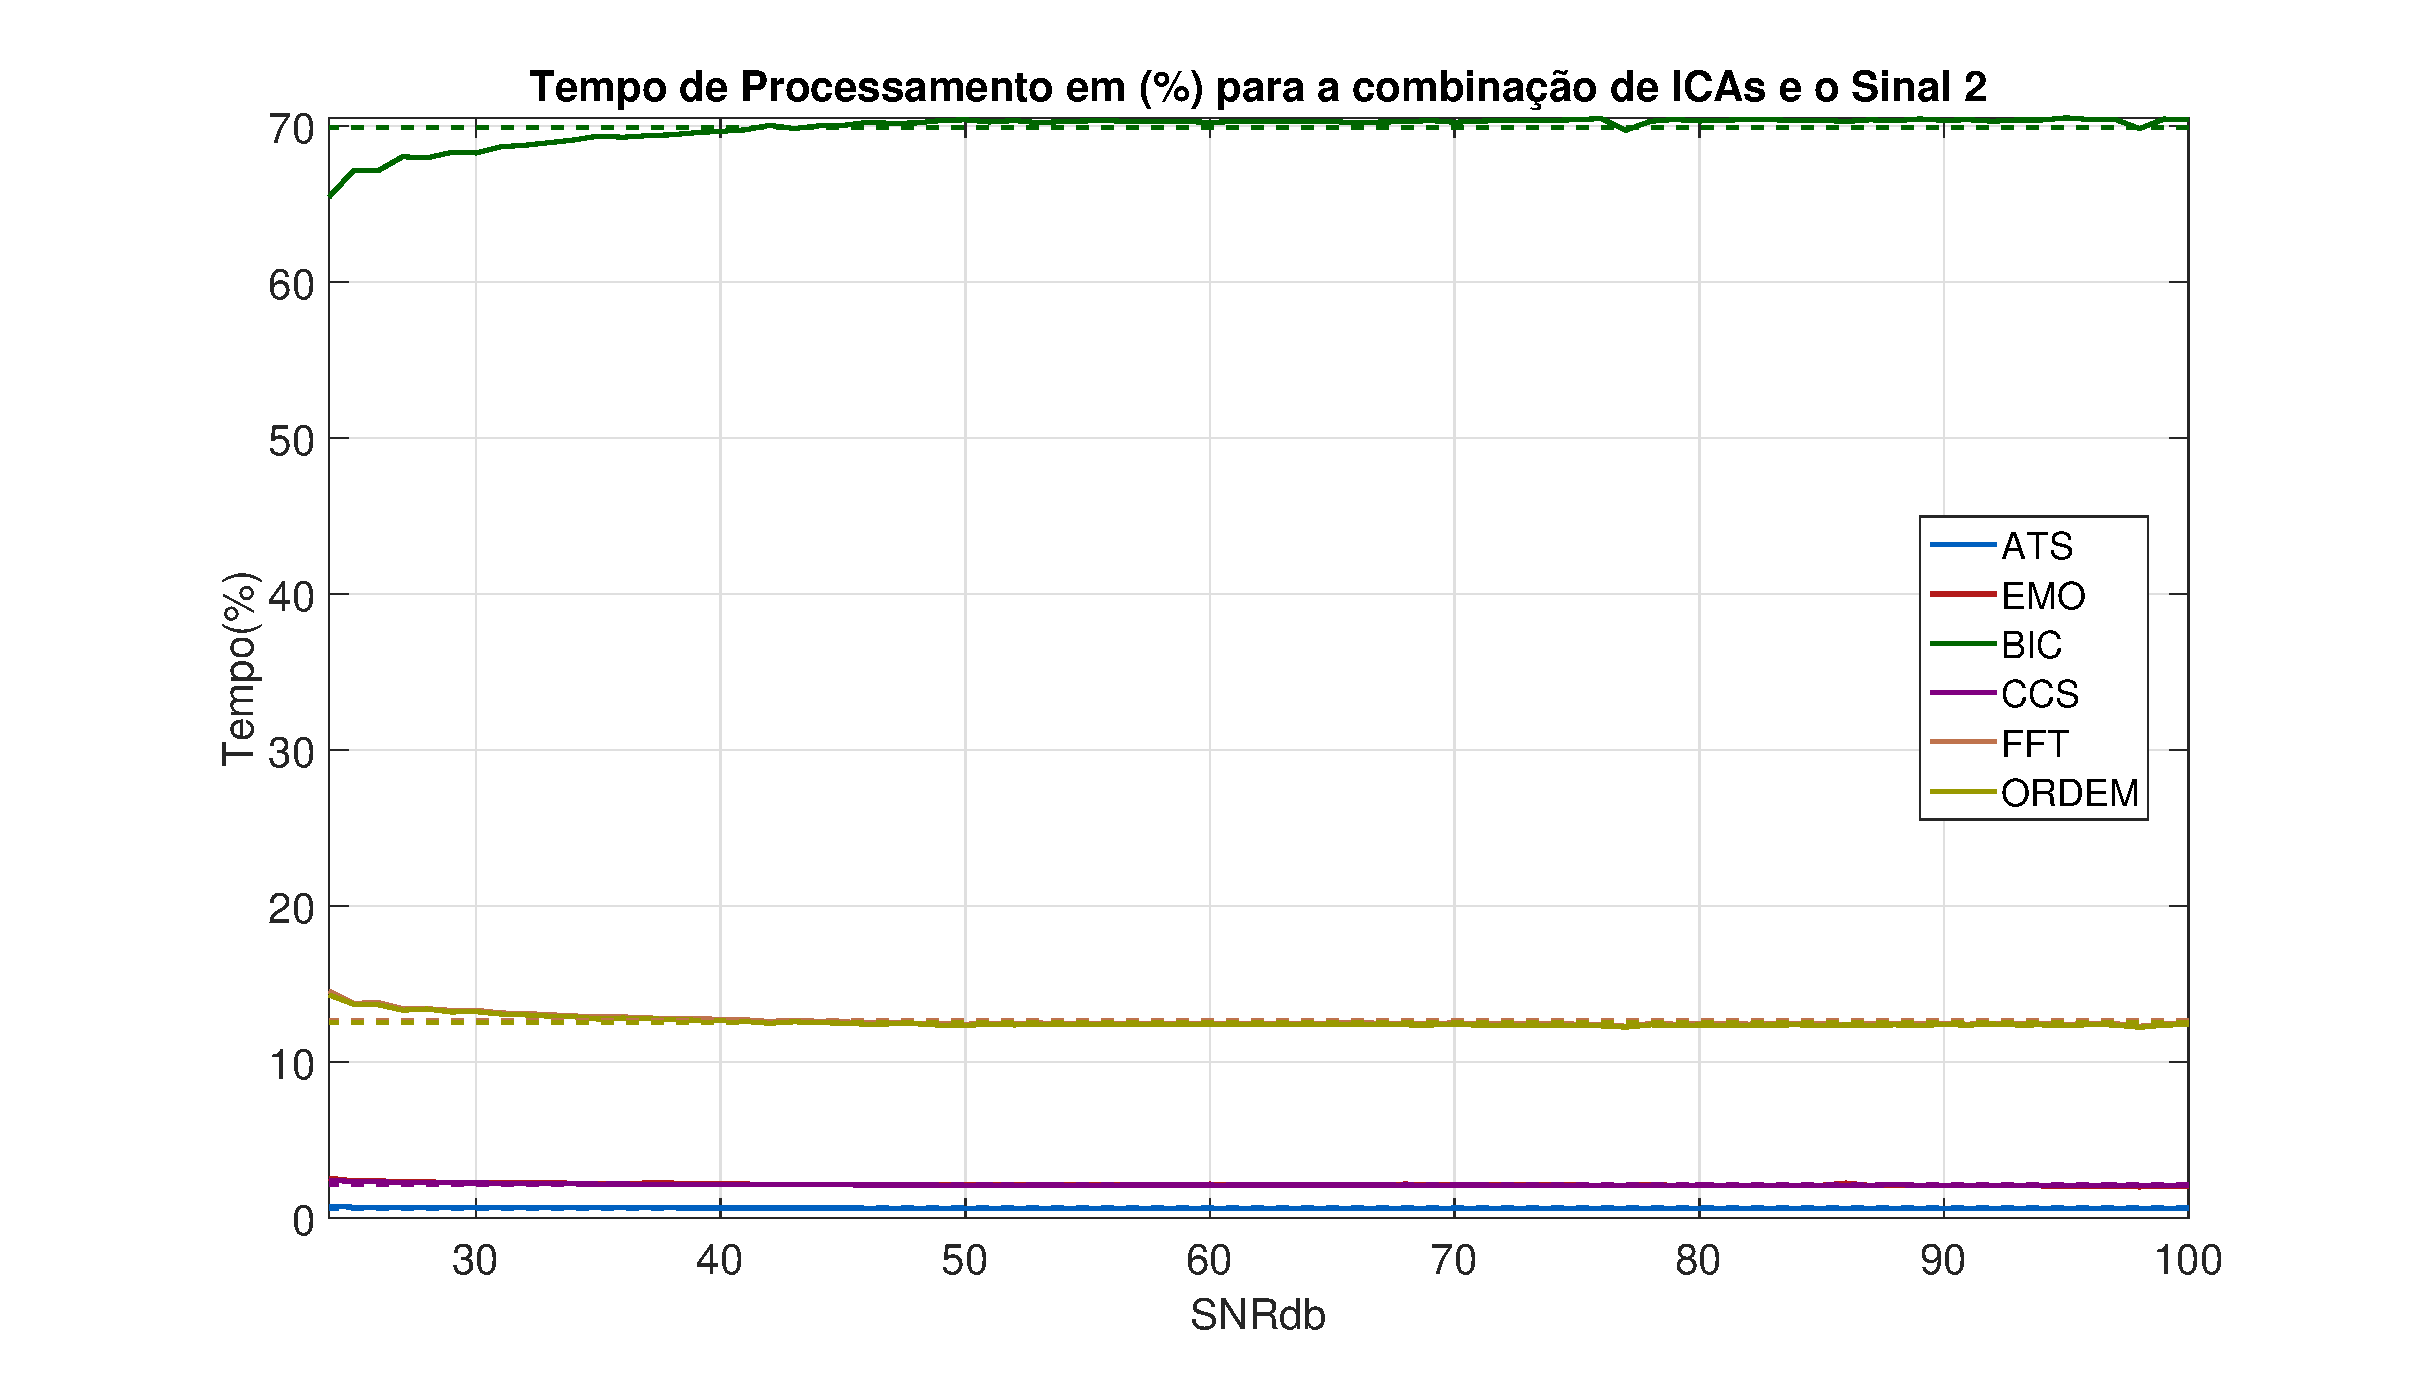
\includegraphics[scale=0.45]{imagens/ImagensParaOAnexo/TPPRCombinacaoICASinal2.eps}
    \caption{TP em porcentagem dos testes para combinação de ICAs em S2.}
    \label{fig:TPCIRS2}    
    \end{center}
\end{figure}

\begin{figure}[!htb]
    \begin{center}
    \advance\leftskip -1.5cm
    \includegraphics[scale=0.45]{imagens/ImagensParaOAnexo/RMSEcompRTodasICAsSinal3.eps}
    \caption{RMSE por componente para as ICAs utilizadas na variação de ruido e o S3.}
    \label{fig:RMSERS3}    
    \end{center}
\end{figure}

\begin{figure}[!htb]
    \begin{center}
    \advance\leftskip -1.5cm
    \includegraphics[scale=0.45]{imagens/ImagensParaOAnexo/TPPRICASOBImodSinal3.eps}
    \caption{TP em porcentagem dos testes para ICA SOBI modificado em S3.}
    \label{fig:TPSMRS3}    
    \end{center}
\end{figure}

\begin{figure}[!htb]
    \begin{center}
    \advance\leftskip -1.5cm
    \includegraphics[scale=0.45]{imagens/ImagensParaOAnexo/TPPRCombinacaoICASinal3.eps}
    \caption{TP em porcentagem dos testes para combinação de ICAs em S3.}
    \label{fig:TPCIRS3}    
    \end{center}
\end{figure}

\begin{figure}[!htb]
    \begin{center}
    \advance\leftskip -1.5cm
    \includegraphics[scale=0.45]{imagens/ImagensParaOAnexo/RMSEcompRTodasICAsSinal4.eps}
    \caption{RMSE por componente para as ICAs utilizadas na variação de ruido e o S4.}
    \label{fig:RMSERS4}    
    \end{center}
\end{figure}

\begin{figure}[!htb]
    \begin{center}
    \advance\leftskip -1.5cm
    \includegraphics[scale=0.45]{imagens/ImagensParaOAnexo/TPPRICASOBImodSinal1.eps}
    \caption{TP em porcentagem dos testes para ICA SOBI modificado em S4.}
    \label{fig:TPSMRS4}    
    \end{center}
\end{figure}

\begin{figure}[!htb]
    \begin{center}
    \advance\leftskip -1.5cm
    \includegraphics[scale=0.45]{imagens/ImagensParaOAnexo/TPPRCombinacaoICASinal4.eps}
    \caption{TP em porcentagem dos testes para combinação de ICAs em S4.}
    \label{fig:TPCIRS4}    
    \end{center}
\end{figure}

\begin{figure}[!htb]
    \begin{center}
    \advance\leftskip -1.5cm
    \includegraphics[scale=0.45]{imagens/ImagensParaOAnexo/RMSEcompRTodasICAsSinal5.eps}
    \caption{RMSE por componente para as ICAs utilizadas na variação de ruido e o S5.}
    \label{fig:RMSERS5}    
    \end{center}
\end{figure}

\begin{figure}[!htb]
    \begin{center}
    \advance\leftskip -1.5cm
    \includegraphics[scale=0.45]{imagens/ImagensParaOAnexo/TPPRICASOBImodSinal5.eps}
    \caption{TP em porcentagem dos testes para ICA SOBI modificado em S5.}
    \label{fig:TPSMAS5}    
    \end{center}
\end{figure}

\begin{figure}[!htb]
    \begin{center}
    \advance\leftskip -1.5cm
    \includegraphics[scale=0.45]{imagens/ImagensParaOAnexo/TPPRCombinacaoICASinal5.eps}
    \caption{TP em porcentagem dos testes para combinação de ICAs em S5.}
    \label{fig:TPCIRS5}    
    \end{center}
\end{figure}


\end{document}
